\documentclass[a4paper, 12pt]{book}
%; whizzy -pdf
\usepackage[T2A]{fontenc}
\usepackage[utf8]{inputenc}
\usepackage[english, russian]{babel}
\usepackage{upquote}
\usepackage{textcomp}
\usepackage[pdftex]{graphicx}
\graphicspath{{cover/}}
\usepackage{pdfpages}
\usepackage[pdfborder={0 0 0}]{hyperref}
\title{Let Over Lambda \\50 Лет Лиспу}
\date{2008}
\author{Даг Хойт}

\begin{document}

\newcommand{\listbegin} {\hrule}
\newcommand{\listend} {\hrule\vspace{0.1cm}}


%\thispagestyle{empty}
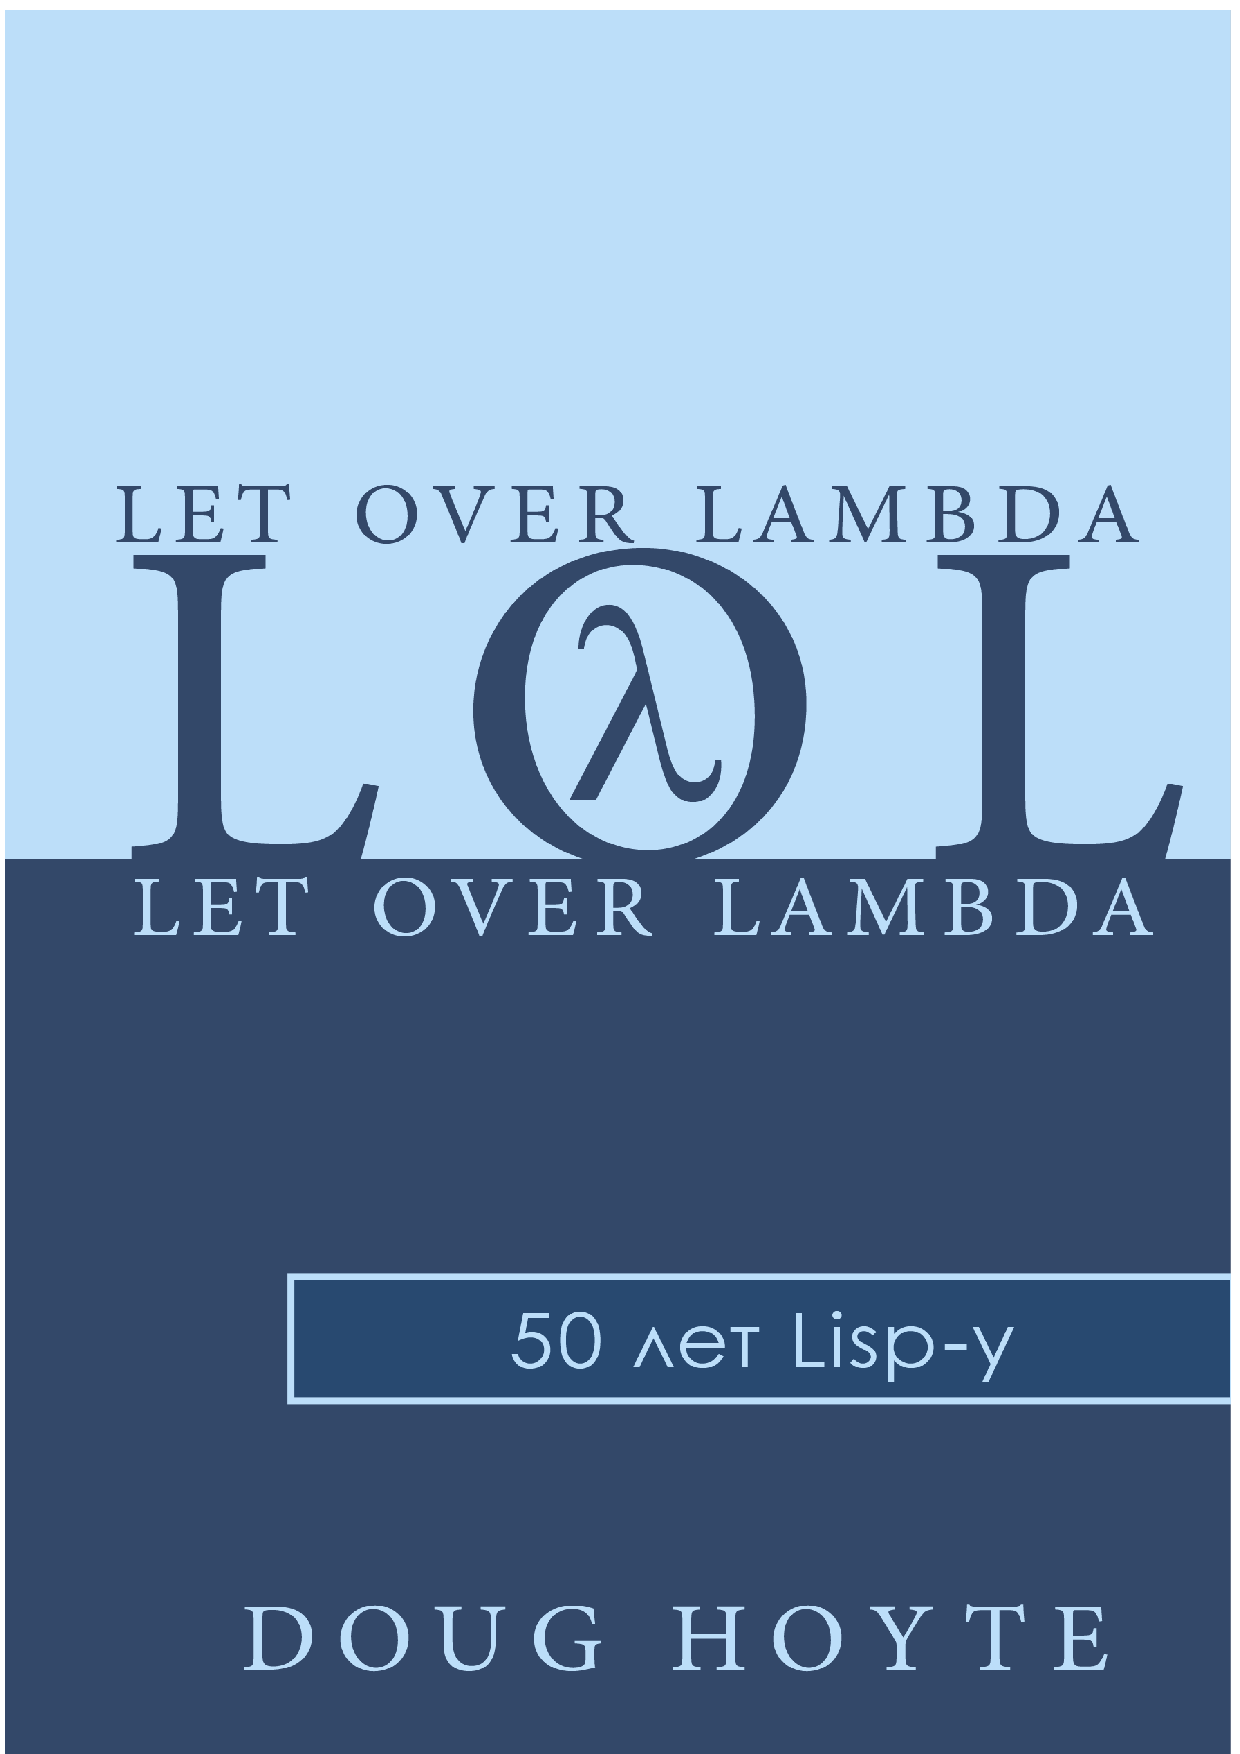
\includepdf[pages={1}]{cover/first_page.pdf}



%\pagestyle{headings}


\renewcommand {\contentsname} {Оглавление}
\renewcommand {\chaptername} {Глава}
%\hyphenation{уво-дя-щая}
\hyphenation{по-вес-тво-ва-ние}
\hyphenation{де-мон-стри-ро-вать}
\hyphenation{ис-поль-зо-ва-ние}
\hyphenation{свойс-тва}
\hyphenation{за-бав-ные}
\hyphenation{вы-чис-ле-ния}
\hyphenation{ко-ли-чес-тво}
\hyphenation{прос-мат-ри-вать}
\hyphenation{сба-лан-си-ро-ванным}
\hyphenation{Ник-то}
\hyphenation{выпол-не-нии}
\hyphenation{прог-рам-мы}
\hyphenation{Пос-редс-твен-ность}
\hyphenation{раз-дра-жаю-щей}
\hyphenation{прод-ви-ну-той}
\hyphenation{изде-ва-тель-ствах}
\hyphenation{добав-ляе-мый}
\hyphenation{мета-прог-рам-миро-ва-нии}
\hyphenation{язы-ках}
\hyphenation{реали-зо-ва-но}
\hyphenation{Пов-то-рить}
\hyphenation{Напе-ча-тать}
\hyphenation{вы-вод}
\hyphenation{сок-ра-щается}
\hyphenation{Вычис-лить}
\hyphenation{при-ме-нять}
\hyphenation{Ник-то}
\hyphenation{про-цесс}
\hyphenation{ите-ра-тив-ный}
\hyphenation{ник-то}
\hyphenation{пот-реб-нос-тями}
\hyphenation{мак-ро-сов}
\hyphenation{тер-ми-но-ло-гии}
\hyphenation{мета-прог-рам-ми-ро-ва-ние}
\hyphenation{един-ствен-ной}
\hyphenation{луч-шие}
\hyphenation{при-сут-ствует}
\hyphenation{пре-вос-ходс-тво}
\hyphenation{мета-прог-рам-мы}
\hyphenation{мета-язы-ки}
\hyphenation{лю-бым}
\hyphenation{тер-ми-ны}
\hyphenation{отли-чается}
\hyphenation{ис-поль-зо-вать}
\hyphenation{сим-во-ли-чес-ком}
\hyphenation{абс-трак-ций}
\hyphenation{ре-али-зо-ва-на}
\hyphenation{биб-лио-те-ку}
\hyphenation{стан-дар-ти-зуются}
\hyphenation{слоя-ми}
\hyphenation{проб-ле-ма}
\hyphenation{поль-зо-ва-те-лям}
\hyphenation{спроек-ти-ро-ва-на}
\hyphenation{спроек-ти-ро-ван-ных}
\hyphenation{произ-во-ди-тель-нос-тей}
\hyphenation{сим-во-лов}
\hyphenation{от-ли-чие}
\hyphenation{со-дер-жа-щий}
\hyphenation{воз-вра-щать}
\hyphenation{стан-дар-тную}
\hyphenation{прог-рам-ми-ро-вать}
\hyphenation{стан-дар-ти-зи-руются}
\hyphenation{сло-ями}
\hyphenation{пре-дос-тав-ляет-ся}
\hyphenation{боль-ше}
\hyphenation{прог-рам-мное}
\hyphenation{раз-но-вид-ность}
\hyphenation{раз-но-вид-нос-тям}
\hyphenation{боль-ше}
\hyphenation{При-ло-же-ние}
\hyphenation{ос-таёт-ся}
\hyphenation{преж-не-му}
\hyphenation{пре-вы-си-ть}
\hyphenation{вы-ра-щен-ны-ми}

\maketitle
\begin{center}
{\LARGE $\lambda$}


Let Over Lambda

50 лет Лиспу

Даг Хойт (Doug Hoyte)

Let Over Lambda

Редакция 1.0

Авторские права принадлежат Дагу Хойту (Doug Hoyte)

Все права защищены

Авторские права на код принадлежат Дагу Хойту (Doug Hoyte)

Никакие права не зарегистрированы

ISBN: 978-1-4357-1275-1

http://letoverlambda.com

doug@hcsw.org

Производство HCSW и Hoytech

Сделано на Lisp-е

Автор перевода: Charlz\_Klug

Русификация обложки: Илья (Zirom) Сёмин. E-mail: zirom@list.ru

Вёрстка, вычитка седьмой главы и перевод восьмой главы: Алексей Фокин.
\end{center}
\tableofcontents
\chapter{Введение}\label{chapter_introduction}
\section{Макросы}\label{section_macros}
\begin{quote}
Ядро Lisp'а занимает в некотором роде локальный оптимум в пространстве языков программирования.

--- Скромные слова Джона МакКарти, создателя Lisp'а
\end{quote}
Эта книга о программировании \emph{макросов} на Lisp-е. Большинство книг о программировании дают лишь беглый обзор материала. Эта книга построена в виде руководств и примеров, написанных таким образом, чтобы вы могли максимально быстро и эффективно программировать сложные макросы. Освоение макросов --- это фи\-наль\-ный шаг, от\-де\-ля\-ющий посредственного Lisp-программиста от Lisp-профессионала.

Макросы --- это единственное самое большое преимущество Lisp-а и единственная важнейшая деталь, которая может присутствовать в дру\-гих языках программирования. С помощью макросов вы можете делать то, что попросту невозможно в других языках. Поскольку макросы могут использоваться для преобразования Lisp-а в другие языки про\-грам\-ми\-ро\-ва\-ния и обратно, то программисты, изучившие макросы, могут обнаружить, что все остальные языки являются просто оболочкой по\-верх Lisp-а. Это \emph{далеко идущий} вывод. Lisp примечателен тем, что программирование на нём --- это программирование на высочайшем уро\-вне. В то время, когда большинство языков изобретают и применяют синтаксические и семантические правила, Lisp универсален и пластичен. С Lisp-ом вы создаёте правила.

История Lisp'а более богата и обширна, нежели история дру\-гих язы\-ков программирования. Над разработкой этого языка работали одни из лучших компьютерных учёных. Благодаря их трудам возник самый мощный и универсальный язык программирования. Lisp содержит много стандартов, несколько замечательных реализаций с открытым исходным кодом и макросы, с которыми не сравнятся другие языки про\-грам\-ми\-ро\-ва\-ния. В этой книге используется только COMMON LISP [ANSI—CL] [CLTL2], но большое количество идей можно легко портировать на такие Lisp'ы, как Scheme[R5RS]. Тем не менее, ознакомившись с этой книгой, вы увидите, что для написания макросов стоит использовать COMMON LISP. В то время, когда остальные Lisp'ы хороши для других целей, COMMON LISP --- это выбор профессионала, работающего с макросами.

Архитекторы COMMON LISP-а проделали замечательную ра\-бо\-ту при про\-ектировании языка. Учитывая качество реализации COMMON LISP, на данный момент, --- это лучшая среда для разработки программ с удивительно малым количеством оговорок. Как программист вы всегда можете рассчитывать на COMMON LISP и будьте уверены что в этом языке всё сделано так, как надо. Несмотря на то, что архитекторы и авторы реализаций выполнили свою работу на отлично, есть пробелы в объяснении того, почему язык реализован таким, а не другим способом. Для многих программистов COMMON LISP --- это огромное коллекция непонятных особенностей, поэтому эти программисты переходят к более привычным, для них, языкам, так и не познав истинной мощи макросов. Эта книга может быть использована в качестве путеводителя по многим замечательным особенностям удивительного языка программирования~---~COMMON LISP. Большинство языков спроектированы так, чтобы их можно было легко реализовать; COMMON LISP спроектирован для соз\-да\-ния мощных программ. Я искренне надеюсь, что создатели COMMON LISP оценят эту книгу как наиболее завершённый и доступный источник сведений об особенностях макросов и что эта книга будет ощутимой каплей в океан тем о макросах.

История макросов начинается почти с историей Lisp-а. Макросы изобретены Тимоти Хартом [MACRO-DEFINITIONS] в 1963 году. Тем не менее, большинство Lisp программистов не используют всю мощь макросов, а остальные программисты вообще не используют макросы. Это всегда остаётся загадкой для продвинутых лисперов. Если макросы настолько хороши, то почему их не используют все программисты? Са\-мые умные и наиболее решительные программисты в конечном счёте приходят к макросам Лиспа. Для того, чтобы понять возможности макросов, необходимо понять что есть в Лиспе и чего нет в других языках. А это в свою очередь требует знания других, менее мощных языков. К сожалению многие программисты теряют желание учиться после того, как они освоят несколько других языков и таким образом никогда не узнают что такое макросы и их возможности. Но, несмотря на это, некоторый процент программистов задумывается над возможностью создания программ, пишущих другие программы --- то есть, они приходят к макросам. А поскольку Лисп --- это лучший язык для создания мак\-ро\-сов, самые умные, самые решительные и самые любознательные про\-грам\-мис\-ты всегда приходят к Лиспу.

Программисты из числа верхнего процентиля всегда будут малым числом, несмотря на то, что общая популяция программистов растёт. Люди из мира программирования видят несколько примеров мощи мак\-ро\-сов, а число людей понимающих макросы ещё меньше, но всё пос\-те\-пен\-но меняется. Поскольку макросы увеличивают производительность в разы, \emph{век макросов} наступает, независимо от того, готов к ним мир или нет. Цель этой книги --- стать первой линией подготовки к неизбежному будущему: миру макросов. Будьте готовы.

Вокруг макросов распространено следующее мнение --- использовать их только при необходимости. Причина этому --- некоторые макросы сложно понимать, в макросы могут закрасться очень трудно оп\-ре\-де\-ляемые ошибки и в случае, когда вы обо всём думаете как о функциях, то макросы могут вас неприятно удивить. Это не дефекты Лисповской системы макросов, а общие черты программирования макросов. Как и в случае с любой технологией: чем более мощен инструмент --- тем больше способов его неправильного использования. А среди всех программных конструкций макросы Лиспа --- это наиболее мощный инструмент.

Можно провести параллель между изучением макросов в Лиспе и изучением указателей в языке программирования C. Большинство на\-чи\-наю\-щих программистов C легко усваивают большую часть языка. Фун\-к\-ции, типы, переменные, арифметические выражения: все они имеют параллели с предыдущим интеллектуальным опытом начинающих прог\-рам\-мис\-тов, начиная с математики уровня начальной школы и за\-кан\-чивая экспериментами с простейшими языками программирования. Но, большинство новичков в C упираются в кирпичную стену при изучении указателей.

Указатели являются второй натурой опытного C программиста. Мно\-гие опытные C программисты считают что полное понимание указателей необходимо для правильного использования C. Поскольку указатели яв\-ляю\-тся фундаментальной идеей, многие опытные C программисты не рекомендуют ограничивать использование указателей при обучении или для стилистической красоты. Несмотря на это многие новички в C считают указатели ненужным усложнением и избегают их ис\-поль\-зо\-ва\-ния, так возникает \emph{симптом FORTRAN-а (пренебрежение полезными особенностями ''вне за\-ви\-си\-мос\-ти от я\-зы\-ка'')}. Бо\-лез\-нью является иг\-но\-ри\-ро\-ва\-ние особенностей языка, а не плохой программистский стиль. Если же особенности языка освоены в полном объёме, то корректный стиль программирования становится очевидным. Не нужно стремиться выработать какой-либо стиль программирования, это касается всех я\-зы\-ков, --- вспомогательная тема этой книги. Стиль нужен только в том случае, когда отсутствует понимание\footnote{Следствие этого --- эффективное использование чего-ли\-бо од\-но\-го, подсмотренного где-либо, способом при отсутствии должного понимания природы вещей.}.

Подобно указателям C, макросы --- это особенность Лиспа, которая часто остаётся плохо понятой, и поэтому распространены не совсем вер\-ные представления о макросах. Если при работе с макросами вы по\-ла\-гаетесь на такие высказывания как:

\begin{quote}
Макросы изменяют синтаксис Лисп кода.

Макросы работают в дереве разбора ваших программ.

Используйте макросы только тогда, когда с задачей не справ\-ляются функции.
\end{quote}
то скорее всего вы упустили из виду общую картину, что даёт прог\-рам\-ми\-ро\-вание макросов. Именно это и исправляет эта книга.

Хорошие справочники и руководства по макросам можно пересчитать по пальцам. Одним из хороших книг по макросам является книга Пола Грэма \emph{On Lisp} [On-Lisp]. Рекомендуется к прочтению от корки до корки всем, кто интересуется макросами. \emph{On Lisp} и остальные труды Грэма послужили толчком к написанию книги, которую вы сейчас читаете. Благодаря Полу Грэму и остальным людям, писавшим о Лиспе, мощь макросов широко обсуждается, но, к сожалению, всё же остаётся также широко не понятой. Несмотря на то, что просто прочитав книгу \emph{On Lisp} можно узнать много интересного о макросах, некоторые программисты связывают проблемы программирования с макросами. В то время, когда \emph{On Lisp} показывает вам различные виды макросов, эта книга расскажет вам как использовать эти макросы.

Написание макросов --- это итеративный процесс, связанный с раз\-мыш\-ле\-ниями. Все сложные макросы начинаются из простых макросов, прошедших через долгую серию улучшений и тестирований. Кроме того, знание о том, где применить макросы приходит с накоплением опыта написания макросов. При написании программ человек следует не\-ко\-торой системе и процессу. Каждый программист представляет себе не\-кую концептуальную модель работы инструментов программирования и создаёт код исходя из результатов вытекающих из этой модели. Про\-грам\-мист, обладающий интеллектом начнёт задумываться о прог\-рам\-ми\-ро\-ва\-нии, как о логической процедуре, и придёт к мысли, о процессе автоматизации программирования. После этого программист будет го\-то\-ви\-ться к процессам автоматизации.

Важным шагом к пониманию макросов является следующее: если писать код без тщательного планирования и без приложения зна\-чи\-те\-льных усилий, то в результате код будет нашпигован множественными шаблонами и негибкими абс\-трак\-циями. Такое положение вы можете увидеть в любых больших программах. Дублируемые участки кода и слишком усложнённый код --- это отсутствие правильных абстракций у авторов кода. Эффективное использование макросов подразумевает под собой признание проблемы в виде повторяющихся шаблонов и абс\-трак\-ций, после этого следует создание \emph{кода, помогающего вам писать код}. Но этого не достаточно для того, чтобы понять как писать макросы; профессиональный Лисп программист хочет знать зачем писать мак\-ро\-сы.

Программисты на C, только пришедшие в Лисп, часто делают ошибку считая что главное предназначение макросов в улучшении эффек\-тив\-ности кода в момент выполнения\footnote{Программисты на C делают эту ошибку по причине того, что "макро система" действительно хороша для этих целей, но главное назначение макросов не в этом.}. Да, довольно часто макросы ис\-поль\-зуются именно для этой задачи, но наиболее общей целью использования макросов является упрощение процесса программирования. В боль\-шинс\-тве программах шаблоны просто избыточно копируются, а абстракции используются в не достаточной мере, правильно спроектированные мак\-ро\-сы могут вывести выразительность программирования на ещё боль\-ший уровень. Там, где остальные языки оказываются ограниченными и конкретными, Лисп остаётся универсальным и гибким.

Эта книга не введение в Лисп. Темы и материал подобраны для профессиональных программистов в не-Лисп языках, интересующихся пользой, которую можно извлечь из макросов и для студентов, пос\-редс\-твен\-но знающих Лисп, которые готовы по настоящему изучить самую сильную сторону Лиспа. Подразумевается, что вы посредственно знаете Лисп, и от вас не требуется глубокого знания замыканий и макросов.

Эта книга не только о теории. Все примеры, приведённые здесь, полностью функциональны, пригодны для использования и могут по\-мочь вам улучшить ваше программирование здесь и сейчас. Эта книга о применении передовых программистских технологий для улучшения вашего программирования. Во многих книгах посвящённых прог\-рам\-ми\-ро\-ва\-нию сознательно применяется простой стиль программирования в угоду доступности. В этой книге материал преподаётся с полным применением всего языка. Кроме этого приведённые примеры кода ис\-поль\-зуют эзотерические особенности COMMON LISP, большинство из которых будут описываться при использовании. Если вы прочитали и поняли\footnote{Конечно, вы можете не соглашаться с этим утверждением.} всё, что описано в \emph{главе 2, Замыкания, на странице \pageref{chapter_closures}} и в \emph{главе 3, Основы Макросов, на странице \pageref{chapter_macro_basics}}, то можете считать что вы прошли среднюю стадию понимания Лиспа.

Одной из частей Лиспа является самостоятельные открытия, эта кни\-га не лишит вас удовольствия от экспериментов. Имейте в виду, что материал в этой книге подаётся очень быстро, много быстрее, чем вы сможете усвоить. Для того, чтобы понять некоторые участки кода, приведённые здесь, вам придётся обращаться к другим справочникам и руководствам по COMMON LISP'у. После изучения базовых понятий мы перейдём прямо к последним исследованиям, посвящённым макросам, большинство из которых граничат с большой неизведанной областью. Эта книга фокусируется на \emph{комбинировании макросов}. Эта тема имеет пугающую репутацию, а хорошо понять эту тему способны не все прог\-рам\-мисты. Комбинирование макросов включает в себя наиболее об\-шир\-ные и плодородные исследования в языках программирования. Ис\-сле\-до\-ва\-те\-лями было выжато почти всё из типов, объектов и пролого-подобной логики, но программирование макросов остаётся огромной, зияющей чёрной дырой. Никто не знает до конца что лежит по ту сторону. Всё, что мы знаем на данный момент --- это то, что макросы сложны, пугающи и проявляют неограниченный потенциал. В отличие от многих программистских идей макросы не являются ни ака\-де\-ми\-ческой концепцией для производства бесполезных теоретических пуб\-ли\-каций, ни пустым модным словом относящемуся к программному обес\-пе\-че\-нию компаний. Макросы --- это лучшие друзья хакеров. Макросы делают ваши программы умнее, а не труднее. Большинство прог\-рам\-мис\-тов, начавших изучение макросов приходят к выводу что прог\-рам\-ми\-ро\-ва\-ние без макросов --- это не программирование.

Многие книги посвящённые Лиспу написаны в пропагандистском ключе, но я совершенно равнодушно отношусь к публичным призывам использовать Лисп. Лисп не собирается уходить. Я был бы счастлив если бы мог использовать Лисп в качестве \emph{секретного оружия} на про\-тя\-же\-нии всей своей карьеры программиста. Эта книга имеет только одну цель --- вдохновить на изучение и исследование, также, как я был вдохновлён \emph{On Lisp}'ом. Я надеюсь, что смогу вдохновить читателей этой книги и смогу насладиться ещё более лучшими Лисповскими макро инструментами и ещё более интересными книгами о макросах Лиспа.

Да пребудет с вами сила Лиспа,

ваш покорный автор,

Даг Хойт.
\section{U-Язык}\label{section_u_language}
Обсуждение макросов влечёт за собой обсуждение обсуждения, поэтому мы должны чётко обозначить соглашения, используемые в этой книге. Всё, что я сейчас пишу и всё что вы получаете из книги через чтение и интерпретацию прочитанного, что в свою очередь представляет из себя систему выражений подлежащих формализации и анализу.

Никто не понимает этого лучше, чем Хаскелл Карри, автор \emph{Основ Математической Логики} [FOUNDATIONS]. Карри, который пытался не просто формализовать идеи, а формализовать ещё и само выражение идей, посчитал необходимым абстрагировать эту концепцию в ком\-му\-ни\-ка\-тив\-ный язык между писателем и читателем. Он назвал его U-Язык (U-Language).

\begin{figure}Листинг 1.1: ПРИМЕР-ЛИСТИНГА-ПРОГРАММЫ\label{listing_1.1}
\listbegin
\begin{verbatim}
(defun example-program-listing ()
  '(this is
    (a (program
        (listing)))))
\end{verbatim}
\listend
\end{figure}

\begin{quote}
Каждое исследование, включая эту книгу, должны пе\-ре\-да\-ва\-ться от одного человека к другому через язык. Целесообразно начать наше обучение обратив внимание на тот очевидный факт, что нужно дать некоторое имя нашему языку и явно обозначить его функции. Мы будем называть наш ис\-поль\-зуемый язык U-Языком. [...] Если бы язык не был так тесно связан с нашей работой, то можно было бы не уделять ему такого внимания.
\end{quote}

На протяжении всей книги мы будем вводить новые ключевые кон\-цеп\-ции или будем обращать внимание на какой-либо момент \emph{вот таким шриф\-том}. При цитировании специальных форм, функций, макросов и других иден\-тификаторов присутствующих в уже встреченных или ещё не опи\-сан\-ных программах, мы будем использовать \textbf{этот спе\-циаль\-ный шри\-фт} (уч\-тите что некоторые слова имеют множественные значения, на\-при\-мер мак\-рос \textbf{lambda} в COMMON LISP и концепция лямбда; спе\-циаль\-ная форма \textbf{let} и список, представляющую формы).

В этой книге новые куски кода представлены в форме \emph{листингов программ}. Код, который можно использовать в своих программах или примеры соответствующих реализаций, выделены в определении наших функций так: \textbf{example-program-listing}. Но иногда мы будем демонстрировать использование некоторого кода или просто обсуждать свойства некоторых выражений с шрифтом текста книги\footnote{А это сноска, имеющая отношение к основному тексту, но, уводящая повествование в сторону.}. В этих случаях код или примеры использования кода будут отображаться так:

\begin{verbatim}
(this is
  (demonstration code))
\end{verbatim}

В большинстве книг о программировании приводятся изолированные, искусственные примеры, и в то же время авторы забывают связывать эти примеры с реальной жизнью. Примеры в этой книге очень короткие и связаны с общей картиной преподаваемых идей программирования. Некоторые авторы пытаются скрасить скуку примеров используя забавные и хитрые идентификаторы имён или поверхностные аналогии. Наши примеры служат лишь для иллюстрации идей. Но это не значит что вся книга позиционируется как очень серьёзная. Здесь присутствует юмор, но нужно суметь его найти.

Поскольку Лисп имеет интерактивную природу, результат вычисления простого выражения часто передаёт больше чем соответствующее количество информации в U-Языке. В этих случаях мы будем применять вывод из COMMON LISP-овс\-кого Прочитать Вычислить Напечатать Повторить ( Read Evaluate Print Loop --- сокращается до REPL ):

\begin{verbatim}
 * (это
    (выражение
      (для вычисления)))

 ЭТО-РЕЗУЛЬТАТ
\end{verbatim}

Обратите внимание: текст кода введён в нижнем регистре, а текст возвращённый Лиспом в верхнем регистре. Эта особенность COMMON LISP, что позволяет нам легко вычленять вывод REPL от введённых выражений. Точнее, эта особенность позволит нам быстро просматривать Лисп формы, содержащие символы --- в каком-либо файле или экране --- и сразу узнать во что они были вычислены Лисп считывателем. Кроме того, заметьте, что в приглашении присутствует символ астериска (*). Этот символ идеален, поскольку его нельзя перепутать со сбалансированным символом и его начертание позволяет быстро определить его в сессии REPL.

Написание сложных Лисп макросов --- это \emph{итеративный} процесс. Ни один человек не может просто так взять и выдавать очередями уже готовые макросы величиной с целую страницу. Этому есть две причины: при сравнении большинства других языков, Лисп программа при равном объёме кода содержит гораздо больше информации, вторая причина в том, что Лисп поощряет программистов в итеративной разработке программ: выполнении серии улучшений, продиктованной потребностями создаваемой программы.

В этой книге используется разделение между такими диалектами Лиспа, как COMMON LISP и Scheme и более абстрактными Лиспами, используемыми в качестве строительного материала. Другое важное отличие, используемое в этой книге --- это проведение границы между диалектами Лиспа и не-Лисп языками программирования. Иногда, нам нужно будет говорить о не-Лисповских языках программирования, для того чтобы нажить как можно больше врагов, мы будем избегать упоминания какого-либо конкретного языка. Мы используем следующее необычное утверждение:

\begin{quote}
Язык без Лисп макросов называется Блаб.
\end{quote}

Слово Блаб в U-Язык пришло из эссе Пола Грэма, \emph{Побеждая Посредственность} [BEATING-AVGS], где Блаб --- это гипотетический язык, используемый для выделения того факта, что Лисп отличается от других языков: Лисп --- другой. Блаб характеризуется инфиксным синтаксисом, раздражающей системой типов, увечной объектной системой, но самая главная черта, объединяющая Блаб языки --- это отсутствие Лисп макросов. Ещё одна полезная сторона Блаба --- в том, что простейший способ изучения продвинутой технологии макросов --- это рассмотрение причин по которой макросы невозможно использовать в Блабе. Цель Блаб терминологии не в издевательствах над не Лисп языками\footnote{Хотя в этом есть доля юмора.}.

Для иллюстрации итеративного процесса создания макроса, в этой книге используется следующее соглашение: символ процента (\%), добавляемый к именам обозначает не завершённость или возможность какого-либо улучшения функций или макросов. С каждым улучшением к имени будет добавляться ещё один символ \% и так до тех пор, пока мы не придём к финальному варианту. Финальный вариант будет без символов процента.

В терминологии Карри макросы описываются как \emph{метапрограммирование}. Метапрограммирование --- это программа, созданная с единственной целью --- дать возможность программисту писать ещё более лучшие программы. Метапрограммирование, в том или ином виде присутствует во всех языках программирования, но ни в одном языке метапрограммирование не реализовано так хорошо как в Лиспе. Ни в одном другом языке нельзя так удобно писать программы с помощью техник метапрограммирования. Именно поэтому Лисп программы выглядят так \emph{странно} для не-Лисп программистов: Лисп код выражен как прямое следствие нужд метапрограммирования. В этой книге мы попытаемся описать это архитектурное решение Лиспа --- создание метапрограмм на самом же Лиспе --- деталь, которая даёт Лиспу потрясающее превосходство в продуктивности. Однако, поскольку мы будем создавать метапрограммы в Лиспе, мы должны помнить, что метапрограммирование отличается от спецификаций U-Языка. Мы могли бы обсуждать метаязыки с различных точек зрения, включая остальные метаязыки, но здесь у нас есть только U-Язык. Комментарий Карри по поводу своей системы:

\begin{quote}
Мы можем продолжить формировать иерархию языков с любым числом уровней. Однако, вне зависимости от количества уровней U-Язык будет находиться на самом высоком уровне: если есть два уровня, то это будет мета-язык; если есть три уровня, то будет мета-мета-язык; и т.д. Таким образом термины U-Языка и мета-языка должны различаться.
\end{quote}



\begin{figure}Листинг 1.2: ПРИМЕР-ИТЕРАТИВНОГО-ПРОЦЕССА\label{listing_1.2}
\listbegin
\begin{verbatim}
(defun example-function% () ; первая версия
  t)

(defun example-function%% () ; вторая версия
  t)

(defun example-function () ; финальная версия!
  t)
\end{verbatim}
\listend
\end{figure}

Эта книга о Лиспе, конечно, логическая система Лиспа очень отличается от системы, которую описал Карри, поэтому мы будем использовать ещё и несколько других идей из его работы. Но, вклад Карри в логику и метапрограммирование продолжает вдохновлять нас и по сей день. Не только благодаря его фундаментальным идеям о символическом закавычивании (symbolic quotation), но и благодаря красиво описанном и выполненном U-Языке.
\section{Утилиты Лисп}\label{section_the_lisp_utility}

\emph{On Lisp} --- это одна из тех книг, которую вы либо поймёте, либо не поймёте. \emph{On Lisp} вы либо будете обожать, либо будете бояться. Начиная с самого названия \emph{On Lisp} рассказывает о создании программных абстракций, находящихся \emph{на верхнем слое Лиспа}. После создания этих абстракций мы можем создать ещё один слой абстракций над абстракциями.

В большинстве языках большая часть функциональности языка реализована на самом языке; обычно Блаб языки имеют при себе стандартную библиотеку написанную на Блабе. Если авторы языка не хотят программировать на самом языке, то, возможно, вы тоже не захотите писать программы на таком языке.

Даже если в другие языки добавить стандартные библиотеки, Лисп всё равно остаётся другим. Другие языки составлены из примитивов, а Лисп составлен из мета-примитивов. Как только макросы стандартизируются, как в COMMON LISP'е, то весь остальной язык можно \emph{создать} из, практически, ничего. Для гибкости в большинстве языках используются наборы примитивов, Лисп же предоставляет нам систему мета-программирования, в свою очередь дающую доступ к любым разновидностям примитивов. Можно взглянуть и с другой точки зрения: Лисп вообще устраняет всю концепцию примитивов. В Лиспе система мета-программирования не останавливается на каких-либо примитивах. В Лиспе возможно, а по факту --- желательно, используя технику макро программирования, развить язык в пользовательское приложение. Приложение, доработанное до самого высокого пользовательского уровня, по прежнему остаётся слоями из макросов на луковице Лиспа, выращенными через итерации.

В этом свете присутствие примитивов в языке выглядит как проблема. В архитектуре системы всегда присутствуют примитивы, барьеры, не ортогональность. Конечно, иногда это оправдано. Для большинства программистов не является проблемой обработка отдельных машинных кодов как примитивов в C или Лисп компиляторах. Но Лисп пользователям нужен контроль над всем. Ни в одном другом языке не предоставляется такой полный контроль программисту над языком как в Лиспе.

\begin{figure}Листинг 1.3: MKSTR-SYMB\label{listing_1.3}
\listbegin
\begin{verbatim}
(defun mkstr (&rest args)
  (with-output-to-string (s)
    (dolist (a args) (princ a s))))

(defun symb (&rest args)
  (values (intern (apply #'mkstr args))))
\end{verbatim}
\listend
\end{figure}

По совету из книги \emph{On Lisp}, книга, которую вы сейчас читаете спроектирована как ещё один слой луковицы. Так же, как одни программы представляют слой над другими программами, эта книга базируется на \emph{On Lisp}. Это центральная тема книги Грэма: при сочетании хорошо спроектированных \emph{утилит} общая производительность может оказаться большей чем сумма производительностей каждой утилиты. Этот раздел описывает коллекцию полезных утилит. Кроме утилит из On Lisp в этот раздел вошли ещё и сторонние утилиты.

Утилита \textbf{symb}, слой поверх \textbf{mkstr} --- основной способ создания символов. Поскольку символы могут ссылаться на любые строки, а программное создание символов чрезвычайно удобно, то \textbf{symb} --- это основная утилита для макро программирования и очень часто используется на протяжении всей книги.

\textbf{Group} --- это другая утилита, постоянно всплывающая при написании макросов. Отчасти это связано с необходимостью в таких отражающих операторах как COMMON LISP'овские \textbf{setf} и \textbf{psetf}, группирующими аргументы, а отчасти и с тем, что часто группировка --- это наилучший путь структурирования связанных данных. Поскольку мы будем очень часто использовать эту функциональность, то эту абстракцию нужно сделать как можно более универсальной. \textbf{Group} Грэма группирует все предоставленное количество групп, определённое в параметре \textbf{n}. В отличие от \textbf{setf}, где аргументы группируются в пары, а \textbf{n} равно 2.

\textbf{Flatten} --- одна из наиболее важных утилит в \emph{On Lisp}. Получает вложенную списковую структуру и возвращает новый список, содержащий списковую структуру всех атомов из начального списка. Если же мы будем думать о списковой структуре как о дереве, то \textbf{flatten} будет возвращать список всех листьев дерева. Если дерево представляет Лисп код, то выполняя некоторую проверку присутствующих объектов в выражении, \textbf{flatten} будет представлять из себя некоторую разновидность \emph{прохода-по-коду (code-walking)} --- тема рекурсии, проходящая через всю книгу.

\begin{figure}Листинг 1.4: GROUP\label{listing_1.4}
\listbegin
\begin{verbatim}
(defun group (source n)
  (if (zerop n) (error "zero length"))
  (labels ((rec (source acc)
             (let ((rest (nthcdr n source)))
               (if (consp rest)
                   (rec rest (cons
                               (subseq source 0 n)
                               acc))
                   (nreverse
                     (cons source acc))))))
    (if source (rec source nil) nil)))
\end{verbatim}
\listend
\end{figure}

\begin{figure}Листинг 1.5: FLATTEN\label{listing_1.5}
\listbegin
\begin{verbatim}
(defun flatten (x)
  (labels ((rec (x acc)
             (cond ((null x) acc)
                   ((atom x) (cons x acc))
                   (t (rec
                        (car x)
                        (rec (cdr x) acc))))))
    (rec x nil)))
\end{verbatim}
\listend
\end{figure}

\begin{figure}Листинг 1.6: FACT-AND-CHOOSE\label{listing_1.6}
\listbegin
\begin{verbatim}
(defun fact (x)
  (if (= x 0)
    1
    (* x (fact (- x 1)))))

(defun choose (n r)
  (/ (fact n)
     (fact (- n r))
     (fact r)))
\end{verbatim}
\listend
\end{figure}

\textbf{Fact} и \textbf{choose} --- это очевидные реализации функций факториала и биномиального коэффициента.

\section{Лицензия}\label{section_license}

Поскольку я считаю что концепции представленные в коде в этой книге являются такими же фундаментальными, как физические наблюдения или математические доказательства, то даже если бы я захотел присвоить их себе, сделать это я бы не смог. По этой причине вы вольны делать с кодом присутствующим в этой книге всё, что угодно. Эта очень либеральная лицензия распространяется вместе с кодом:

\begin{verbatim}
;; Это исходный код для книги
;; _Let_Over_Lambda_ за авторством Дага Хойта.
;; Правообладателем кода является Даг Хойт. 2002-2008 годы.
;;
;; Вы можете свободно использовать, модифицировать и 
;; распространять
;; этот код по вашему желанию, но любые
;; модификации должны быть явно описаны перед
;; распространением. Нет никакой гарантии,
;; явной или косвенной.
;;
;; Приветствуется, но не является обязательным
;; указывание меня, Дага Хойта, в качестве автора кода.
;; Если вы нашли
;; полезным код или хотите получить документацию,
;; пожалуйста, рассмотрите вариант приобретения книги!
\end{verbatim}

Текст этой книги принадлежит Дагу Хойту. 2008 год. Все права защищены.

\section{Благодарности}\label{section_thanks}

Брайан Хойт (Brian Hoyte), Нэнси Холмс (Nancy Holmes), Розали Холмс (Rosalie Holmes), Ян (Ian), Алекс (Alex) и вся остальная моя семья; syke, madness, fyodor, cyb0rg/asm, theclone, blackheart, d00tz, rt, magma, nummish, zhivago, defrost; Майк Конрой (Mike Conroy), Сильвия Рассел (Sylvia Russell), Алан Пэт (Alan Paeth), Роб МакАртур (Rob McArthur), Сильви Десярдинс (Sylvie Desjardins), Джон МакКарти (John McCarthy), Пол Грэм (Paul Graham), Дональд Кнут (Donald Knuth), Лео Броди (Leo Brodie), Брюс Шнайер (Bruce Schneier), Ричард Столлман (Richard Stallman), Эди Вейтз (Edi Weitz), Питер Норвиг (Peter Norvig), Питер Сибель (Peter Seibel), Кристиан Куиннек (Christian Queinnec), Кейт Бостик (Keith Bostic), Джон Гэмбл (John Gamble); проектировщики и создатели COMMON LISP, особенно Гай Стил (Guy Steele), Ричард Гэбриел (Richard Gabriel) и Кент Питман (Kent Pitman), разработчики и сопроводители CMUCL/SBCL, CLISP, OpenBSD, GNU/ Linux.

Отдельная благодарность Яну Хойту (Ian Hoyte) за дизайн обложки и Лео Броди (Leo Brodie) за картинку на обороте обложки.

Эта книга предназначена всем, кто любит программирование.

\chapter{Замыкания}\label{chapter_closures}
\section{Замыкание - Ориентированное Программирование}\label{section_closure-oriented_programming}
\begin{quote}
Один из выводов к которому мы пришли был следующим: "объект" не должен быть примитивным понятием в языке программирования; объекты и их поведение должны строиться из значений ячеек и старых добрых лямбда выражений.

- Гай Стил во время разработки Scheme
\end{quote}

Иногда это называется \emph{замыканием (closure)}, в других случаях - сохранённым лексическим окружением. Или, как любят говорить некоторые из нас - \emph{let, окружающий lambda (let over lambda)}. Вне зависимости от используемой терминологии, усвоение концепции замыканий - это первый шаг в становлении профессионального Лисп программиста. По факту, это умение является жизненно необходимым для правильного использования многих современных языков программирования, кроме этого, сюда можно включить языки явно не поддерживающие let или lambda, например Perl или Javascript.

Замыкания входят в то небольшое число любопытных концепций, парадоксальная сложность которых связана с их чрезвычайной простотой. Когда программист начинает использовать сложные решения проблем, то простые решения начинают казаться ему незавершёнными и неудобными. Далее мы увидим что замыкания могут быть более простым решением нежели решение проблемы в лоб, например организация данных и кода через замыкания может оказаться более простой чем использование объектов. Но, в замыканиях есть ещё более важное свойство чем простота: абстракции, используемые для конструирования макросов - центральная тема этой книги.

Тот факт, что мы можем строить объекты и классы с помощью примитивов замыканий не означает что объектные системы бесполезны для Лисп программистов. Это далеко не так. На самом деле COMMON LISP включает в себя одну из наиболее мощных объектных систем: \emph{CLOS}, COMMON LISP Object System (Объектная Система COMMON LISP). Несмотря на то, что я очень восхищён гибкостью и функциональностью CLOS, его расширенные особенности мне редко бывают нужны\footnote{В COMMON LISP практически невозможно программировать без CLOS, поскольку CLOS занимает центральное место в COMMON LISP.}, благодаря ячейкам с присваиваемыми значениями и старым добрым лямбда выражениям.

В целом эта книга предназначена для программистов со средним уровнем знания Лиспа, но в этой главе мы попытаемся обучить вас с самых основ теории и использованию замыканий, для того, чтобы ознакомить вас с общей терминологией замыканий, используемой на протяжении всей книги. В этой главе рассматривается эффективность замыканий и как современные компиляторы оптимизируют замыкания.

\section{Среды и Просранство}\label{section_environments_and_extent}

Под ячейками с присваиваемым значением Стил определяет среду для сохранения ссылок к данным, где среда - это субъект чего-либо, называемый \emph{неопределённым пространством (indefinite extent)}. Это причудливый способ определения возможности ссылаться на такую среду в любой момент времени. Будучи единожды определённой эта среда и её ссылки будут существовать столько, сколько нам нужно. Рассмотрим следующую C функцию:

\begin{verbatim}
#include <stdlib.h>
int *environment_with_indefinite_extent(int input) {
  int *a = malloc(sizeof(int));
  *a = input;
  return a;
}
\end{verbatim}

После вызова этой функции и получения возвращённого указателя, мы, в течении неопределённого срока, по прежнему можем ссылаться на выделенную память. В C новые среды создаются при вызове функции, но C программисты указывают в \textbf{malloc()} требуемую память при возвращении её для использования за пределами функции.

Для контраста: ниже приведён бесполезный пример. C программисты рассматривают \textbf{a} как автоматически собираемую переменную, происходящее при возвращении функции поскольку среда выделяется в \emph{стеке}. С точки зрения Лисп программистов \textbf{a} создаётся во \emph{вр\'{е}менном пространстве}.

\begin{verbatim}
int *environment_with_temporary_extent(int input) {
  int a = input;
  return &a;
}
\end{verbatim}

Разница между средами C и Лисп в следующем: если вы явно не укажете что вам нужно, то Лисп будет предполагать что вы хотите использовать неопределённое пространство. Другими словами: Лисп всегда предполагает, что вы хотите вызвать \textbf{malloc()}, как в первом примере. Можно сказать, что это по своей природе менее эффективно, чем использование временного пространства, но преимущества почти всегда превышают незначительные издержки производительности. Более того, Лисп сам часто определяет, когда данные могут быть безопасно размещены в стеке и будет делать это автоматически. Вы даже можете использовать \emph{декларации} для того, чтобы Лисп сам явно выполнял эту операцию. Более подробно мы будем обсуждать декларации в \emph{главе 7, Тема Макро Эффективности}.

Но из-за динамичного характера, Лисп не имеет явных значений указателя или типов, как в С. Это может ввести вас в заблуждение, если вы, как программист C, используете вызов указателей и значения для определения типов. Lisp думает обо всем этом немного по-другому. В Лиспе удобно применять следующую мантру:

\begin{quote}
Переменные не имеют типов. Только значения имеют типы.
\end{quote}

Тем не менее, мы должны возвращать что-то для хранения указателей. В Лиспе существуют множество структур данных, которые могут хранить указатели. Одна из самых любимых Лисп программистами простейшей структурой является \emph{ячейка cons (cons cell)}. Каждая cons ячейка содержит ровно два указателя, ласково называемые как \emph{car} и \emph{cdr}. При вызове \textbf{environment-with-indefinite-extent} ячейка \emph{cons} будет вызвана с \emph{car}, указывающим на переданный аргумент \textbf{input}, и \emph{cdr}, указывающий на \textbf{nil}. И что наиболее важно, эта \emph{cons} ячейка (и ссылка на введённый аргумент \textbf{input}) обладает неопределённым пространством, таким образом, мы можем ссылаться на эту ячейку столько, сколько нам нужно:

\begin{verbatim}
(defun environment-with-indefinite-extent (input)
  (cons input nil))
\end{verbatim}

Эффективность недостатков неопределённого пространства достигает неуместности как состояние искусства улучшения технологии Лисп компилирования. Среды и пространства очень тесно связаны с замыканиями. Мы ещё не раз коснёмся темы сред и состояния в этой главе.

\section[Области Видимости]{Лексическая и Динамическая\\ Области Видимости}\label{section_lexical_and_dynamic_scope}

Технический термин, обозначающий доступность ссылки к переменной называется \emph{областью видимости (scope)}. Наиболее общий тип области видимости в современных языках программирования называется \emph{лексической (lexical)} областью. Когда фрагмент кода окружён лексической привязкой к переменной, то говорят что переменная расположена в лексической области привязки. С помощью формы \textbf{let}, наиболее универсальная форма для создания привязок, можно создавать переменные в лексической области:

\begin{verbatim}
* (let ((x 2))
    x)

2
\end{verbatim}

Доступ к \textbf{x} внутри тела формы \textbf{let} осуществляется через лексическую область. Аналогичным образом аргументы в функциях, определённых с помощью \textbf{lambda} или \textbf{defun} являются лексически связанными переменными в тексте определения функции. Лексические переменные - это переменные, доступ к которым возможен только из внутреннего кода контекста, для примера выше, это форма \textbf{let}. Поскольку лексическая область - это чрезвычайно интуитивный способ ограничения доступа к переменной, то может показаться, что это единственный способ разграничения. Есть ли другие другие способы создания областей видимости?

Комбинация неопределённого пространства и лексической области довольно долгое время не использовались в широко распространённых языках программирования. Первая реализация была разработана Стивом Расселом (Steve Russell) для Lisp 1.5 [HISTORY-OF-LISP] и впоследствии спроектирована для таких языков, как Algol-60, Scheme, и COMMON LISP. В Блабах некоторые полезные элементы лексической области видимости стали медленно реализовываться только спустя некоторое время и это несмотря на долгую и познавательную историю лексической области видимости.

Хотя способы реализации областей видимости в C-подобных языках ограничены, C программистам тоже приходится программировать в различных средах. Для этого они используют неявно определённую область видимости, также известную как \emph{область указателя (pointer scope)}. Область указателя известна трудностью в отладке, многочисленными рисками безопасности и, несколько искусственной эффективностью. Идея, лежащая за областью указателей - это создание проблемно-ориентированного языка для контроля регистров и памяти машины фон Неймана, похожей на большинство современных процессоров [PAIP-PIX], с последующим использованием этого языка для доступа и манипулирования структурами данных с непосредственными командами процессора. Область указателей была необходима по причинам производительности во времена, когда Лисп компиляторы ещё не были изобретены, но, теперь, в современных языках программирования область указателей скорее рассматривается как проблема, а не как особенность.

И хотя Лисп программисты редко думают в терминах указателей, понимание областей указателей бывает весьма полезным при создании эффективного Лисп кода. В \emph{разделе Область Указателя} мы будем исследовать реализацию области видимости указателя для тех редких случаев, когда нам нужно уведомить компилятор о создании специфичного кода. Но, в данный момент нам нужно только обсудить механику области указателей. В C нам иногда нужно получать доступ к переменной, определённой за пределом создаваемой функции:

\begin{verbatim}
#include <stdio.h>

void pointer_scope_test() {
  int a;
  scanf("%d", &a);
}
\end{verbatim}

В вышеприведённой функции мы использовали оператор \textbf{\&} в языке C для того, чтобы передать адрес занимаемый в памяти переменной \textbf{a} в функцию \textbf{scanf}, после этого функция \textbf{scanf} знает куда записывать отсканированные данные. Лексическая область видимости в Лиспе запрещает нам напрямую реализовать это действие. В Лиспе нам придётся передать подобную анонимную функцию в гипотетическую Лисп функцию \textbf{scanf}, что позволит ей изменить нашу лексическую переменную \textbf{a}, несмотря на то, что \textbf{scanf} определена за пределами нашей лексической области:

\begin{verbatim}
(let (a)
  (scanf "%d" (lambda (v) (setf a v))))
\end{verbatim}

Лексическая область видимости - это благоприятная среда для замыканий. По факту, замыкания настолько связаны с концепцией лексической области, что часто их более точно называют как \emph{лексические замыкания (lexical closures)}, для того, чтобы отделить их от других видов замыканий. Если не указано что-то другое, то по-умолчанию все замыкания в этой книге являются лексическими.

В дополнение к лексической области в Common Lisp есть ещё и \emph{динамическая область (dynamic scope)}. Это \emph{сленг (slang)} Лиспа обозначающий комбинацию временного пространства и глобальную область. Динамическая область видимости - это одна из разновидности областей видимости. Динамическая область видимости уникальна для Лиспа тем, что предполагает отличающееся поведение с аналогичным синтаксисом лексической области. В Common Lisp переменные, доступные через динамическую область видимости, называются \emph{специальными переменными}. Сделано это для того, чтобы привлечь внимание к таким переменным. Специальные переменные могут быть объявлены с помощью \textbf{defvar}. Некоторые программисты придерживаются соглашения, по которому имена специальных переменных следует начинать и заканчивать символом астериска, например, \textbf{*temp-special*}. Это соглашение называется \emph{"наушник" (earmuff)}. По причинам описанным в \emph{разделе Дуализм Синтаксиса}, эта книга не использует наушники, поэтому наше объявление специальных переменных выглядит так:

\begin{verbatim}
(defvar temp-special)
\end{verbatim}

При таком определении \textbf{temp-special} будет помечен как специальный\footnote{Также мы можем указать с помощью определений локальную особенность.}, но не будет инициализирован каким-либо значением. В этом состоянии специальная переменная называется \emph{несвязанной (unbound)}. Только специальные переменные могут быть несвязанными - лексические переменные всегда связаны и поэтому всегда имеют значения. На это можно взглянуть с другой точки зрения: по-умолчанию все символы представляют из себя лексически не связанные переменные. Также как и с лексическими переменными мы можем присвоить значение специальным переменным с помощью \textbf{setq} или \textbf{setf}. Некоторые Лиспы, такие как Scheme, не имеют динамической области видимости. Другие Лиспы, такие как EuLisp [SMALL-PIECES-P46], используют один синтаксис для доступа к лексическим переменным и другой синтаксис для доступа к специальным переменным. Но в Common Lisp синтаксис общий. Многие лисперы считают это особенностью языка. Так мы присваиваем значение к нашей специальной переменной \textbf{temp-special}:

\begin{verbatim}
(setq temp-special 1)
\end{verbatim}

До сих пор мы не увидели ничего такого, что выделяло бы особенность специальной переменной. Она выглядит как обычная переменная, некоторым образом привязанная к глобальному пространству имени. Всё это потому, что мы только единожды выполнили привязку - специальная глобальная привязка по умолчанию. Специальные переменные интересны тем, что по отношению к ним возможно выполнение повторной привязки, или \emph{затенения (shadowed)}, с помощью новой среды. Мы определим функцию просто вычисляющую и возвращающую \textbf{temp-special}:

\begin{verbatim}
(defun temp-special-returner ()
  temp-special)
\end{verbatim}

Функция может быть использована для получения значения, в которое Лиспом вычисляется \textbf{temp-special} в момент вызова:

\begin{verbatim}
* (temp-special-returner)

1
\end{verbatim}

Иногда это называют вычислением формы в \emph{нулевую лексическую среду (null lexical environment)}. Очевидно, что нулевая лексическая среда не содержит никаких лексических привязок. В данном примере значение \textbf{temp-special} возвращается из глобального специального значения, 1. Но, если мы вычислим его в не-нулевой лексической среде - в той, которая содержит привязку для нашей специальной переменной - то здесь проявится специальность \textbf{temp-special}\footnote{Поскольку мы создаём динамическую привязку, но не лексическую среду. Они просто похожи друг на друга.}:

\begin{verbatim}
* (let ((temp-special 2))
     (temp-special-returner))

2
\end{verbatim}

Обратите внимание, что в качестве значения была возвращена 2, это означает, что значение для \textbf{temp-special} было получено из нашей среды \textbf{let}, а не из специального глобального окружения. Если вам это всё ещё не кажется интересным, то взгляните как это невозможно выразить в большинстве других традиционных языков программирования. Ниже показан пример из псевдокода на Блабе:

\begin{verbatim}
int global_var = 0;

function whatever() {
  int global_var = 1;
  do_stuff_that_uses_global_var();
}

function do_stuff_that_uses_global_var() {
  // global_var is 0
}
\end{verbatim}

Расположение в памяти или значения регистров для лексических привязок становятся известными при компиляции\footnote{По тем же причинам лексическая область видимости называется как "статическая область видимости".}, а привязки для специальных переменных определяются при работе программы. Вам может показаться что специальные переменные не эффективны, но это не так. Специальная переменная всегда ссылается на одно и тоже место в памяти. При использовании \textbf{let}, для привязки специальной переменной, вы на самом деле компилируете код, который сохраняет копию переменной, перезаписывает участок памяти новым значением, вычисляет формы в теле \textbf{let} и, наконец, восстанавливает оригинальное значение из копии.

Специальные переменные постоянно связаны с символом, применяемым для их обозначения. Место в памяти, на которое ссылается специальная переменная называется ячейкой \textbf{символ-значение (symbol-value)} символа. Это прямое противопоставление лексическим переменным. Лексические переменные указываются символами только в момент компилирования. Поскольку доступ к лексическим переменным возможен только изнутри лексической области видимости их привязок, то компилятору нет нужды помнить о символах, применяемых в качестве ссылки на лексические переменные, поэтому компилятор удаляет их из скомпилированного кода. Мы приукрасим истинность этого высказывания в \emph{разделе Пандорические Макросы}.

Хотя Common Lisp и предоставляет нам неоценимые возможности динамической области, но, лексические переменные являются более распространёнными. Раньше динамическая область использовалась для определения особенностей Лиспа, но сейчас, с появлением Common Lisp, почти полностью заменена лексической областью.Поскольку лексическая область позволяет использовать такие приёмы, как лексические замыкания (в дальнейшем мы кратко рассмотрим их), а также более эффективную оптимизацию компилятора, то замена динамической области оказывается хорошей идеей. Однако, архитекторы Common Lisp оставили нам очень прозрачное окно в мир динамической области, которая ныне используется в более узких целях.

\section{Let - это Лямбда}\label{section_let_it_be_lambda}

\textbf{Let} - это специальная Лисп форма для создания среды с именами (привязками), инициализированными в результаты вычисления соответствующих форм. Эти имена доступны для кода внутри тела \textbf{let}, формы в теле \textbf{let} вычисляются последовательно, финальным результатом \textbf{let} является результат вычисления последней формы. Первоочередная задача \textbf{let} - это сам процесс преднамеренной неопределённости. Результат работы \textbf{let} отделён от самой работы \textbf{let}. Так или иначе \textbf{let} нужен для предоставления структуры данных для хранения указателей на значения.

Как мы уже увидели, cons ячейки, несомненно, удобны для хранения указателей, но кроме cons ячеек для хранения указателей можно использовать ещё и другие структуры. Один из лучших путей для хранения указателей в Лиспе - это дать Лиспу возможность самому позаботиться о хранении указателей с помощью формы \textbf{let}. С помощью \textbf{let} вы только указываете имя (привязку) этих указателей, а об остальном позаботится сам Лисп. Иногда мы можем помочь компилятору в создании более эффективного кода, через передачу некоторой информации, добавляемой в форму определения.

\begin{verbatim}
(defun register-allocated-fixnum ()
  (declare (optimize (speed 3) (safety 0)))
  (let ((acc 0))
    (loop for i from 1 to 100 do
          (incf (the fixnum acc)
                (the fixnum i)))
    acc))
\end{verbatim}

В примере \textbf{register-allocated-fixnum} мы дали некоторые подсказки компилятору, что позволяет очень эффективно просуммировать целые числа с 1 до 100. При компиляции эта функция будет располагать данные в регистрах, в целом устраняя необходимость в указателях. Несмотря на то, что с нашей точки зрения мы попросили Лисп создать неопределённую среду для хранения \textbf{acc} и \textbf{i}, Лисп компилятор может оптимизировать эту функцию сохраняя значения прямо в регистрах процессора (CPU). Сгенерированный код может быть таким:

\begin{verbatim}
; 090CEB52:     31C9       XOR ECX, ECX
;       54:     B804000000 MOV EAX, 4
;       59:     EB05       JMP L1
;       5B: L0: 01C1       ADD ECX, EAX
;       5D:     83C004     ADD EAX, 4
;       60: L1: 3D90010000 CMP EAX, 400
;       65:     7EF4       JLE L0
\end{verbatim}

Заметьте, что 4 обозначает 1, а 400 обозначает 100, причина - сдвиг целых чисел на два бита в скомпилированном коде. Это связано с \emph{маркировкой (tagging)} - способ представления чего-либо указателем, а на самом деле использование этого чего-либо для хранения информации. Схема маркировки нашего Лисп компилятора обладает хорошими преимуществами, благодаря которым компилятор не использует сдвиг если индексное слово помещается в памяти [DESIGN-OF-CMUCL]. Подробнее разбор Лисп компилятора будет произведён в \emph{главе 7, Тема Эффективности Макросов}.

Но, если Лисп определит что позже вы можете обратиться к этой среде, то в этом случае будет использоваться что-то менее непостоянное чем регистр. Общей структурой, используемой для хранения указателей в средах, является массив. Если каждая среда имеет массив и все переменные принадлежат этой среде и ссылаются в этот массив, то мы получаем эффективную среду с потенциально неопределённым пространством.

Как было замечено выше, \textbf{let} будет возвращать вычисление последней формы в своём теле. Эта черта объединяет многие специальные формы и макросы Лиспа, такое поведение является настолько общим, что этот шаблон часто называют \emph{неявным progn (implicit progn)} поскольку специальная форма \textbf{progn} реализует именно это поведение\footnote{Progn используется для кластеризации форм и наделяет их высокоуровневым поведением.}. Иногда весьма удобно использовать \textbf{let} форму через возвращение анонимной функции, пользующейся той-же лексической средой, что доступна из формы \textbf{let}. Для создания этих функций в Лиспе мы используем \emph{лямбду (lambda)}.

\emph{Лямбда} - это простая концепция, способная напугать своей гибкостью и важностью. Лямбда, применяемая в Лиспе и Схеме, восходит к логической системе Алонзо Чёрча, но, лямбда получила развитие под спецификацией Лиспа. Лямбда - это короткий способ повторного присваивания временных имён (привязок) к значениям для определённого лексического контекста и лежит в основе концепции Лисп функции. Лисп функция очень отличается от Чёрчевского описания математической функции. Это произошло по причине того, что лямбда развивалась как мощный, практичный инструмент в руках многих поколений лисперов, совершенствующих и расширяющих лямбду до такой степени, предвидеть которую не могли ранние логики.

В лямбде, несмотря на благоговение Лисп программистов, нет ничего особенного. В дальнейшем мы увидим, что лямбда всего лишь один из многих способов выражения этой разновидности именования переменных. В частности, мы увидим, что макросы позволяют нам изменять переименование переменных такими способами, которые абсолютно невозможны в других языках программирования. После изучения таких макросов мы вернёмся к лямбде и обнаружим что лямбда наиболее удобна для оптимального выражения такого рода именования. Это не случайно. С точки зрения программных сред нашего времени Чёрч может показаться устаревшим и неуместным, но на самом деле его вклад нельзя умалить. Его математическая нотация с многочисленными улучшениями в руках многих поколений Лисп профессионалов развилась в универсальный и гибкий инструмент\footnote{Классический пример макроса - это реализация \textbf{let} в лямбда форме. В этой книге я не буду утомлять вас этим примером.}.

Лямбда, как и многие другие особенности Лиспа, очень удобна, самые современные языки начинают импортировать идеи из Лиспа в их собственные системы. Некоторым разработчикам языков кажется что ``lambda'' - это очень длинно, и они начинают использовать такие аббревиатуры как \textbf{fn} и другие. С другой стороны, концепция лямбды настолько фундаментальна, что скрытие этого названия менее длинным именем граничит с ересью. В этой книге мы будем описывать и изучать многие разновидности лямбды и по доброй традиции будем называть лямбду лямбдой так же, как и поколения Лисп программистов до нас.

Но как выглядит лямбда в Лиспе? Прежде всего, как и все имена в Лиспе, лямбда - это \emph{символ (symbol)}. Мы можем закавычивать его, сравнивать его и хранить его в списках. Лямбда обретает специальный смысл только когда появляется в виде первого элемента списка. Если это случится, то список называют \emph{лямбда формой (lambda form)} или \emph{определением функции (function designator)}. Но эта форма - не функция. Эта форма - списковая структура данных, которая может быть преобразована в функцию с помощью специальной формы \textbf{function}:

\begin{verbatim}
* (function '(lambda (x) (+ 1 x)))
#<Interpreted Function>
\end{verbatim}

\footnote{Примечание переводчика: Это выражение приводит к ошибке, возможно здесь подразумевается ``(function (lambda (x) (+ 1 x)))''.}


Для удобства работы с предыдущим выражением в Common Lisp есть сокращение в виде считывающего макроса \verb"#'" (шарп-кавычка). Вместо того, чтобы писать \textbf{function} вы можете получить тот-же эффект с помощью этого сокращения:

\begin{verbatim}
* #'(lambda (x) (+ 1 x))
#<Interpreted Function>
\end{verbatim}

Для большего удобства, лямбда определяется как макрос, расширяющийся в специальную форму с вызовом \textbf{function}, как в примере выше. Стандарт Common Lisp ANSI требует [ANSI-CL-ISO-COMPATIBILITY] чтобы макрос \textbf{lambda} определялся примерно так:

\begin{verbatim}
(defmacro lambda (&whole form &rest body)
  (declare (ignore body))
  `#' ,form)
\end{verbatim}

В данный момент не следует обращать внимание на определение игнорирования\footnote{Определение U-Языка.}. Этот макрос всего лишь простой способ автоматического применения специальной формы \textbf{function} к вашему определению функции. Этот макрос позволяет нам вычислить определение функции для создания функций, поскольку они расширяются в формы шарп-кавычка:

\begin{verbatim}
* (lambda (x) (+ 1 x))
#<Interpreted Function>
\end{verbatim}

Есть несколько веских причин, по которым нужно предварять лямбда формы шарп-кавычкой \verb"#'". Поскольку эта книга не ставит целью поддержку предыдущих сред ANSI Common Lisp, то обратная совместимость соблюдаться не будет. А как же стилистические возражения? Пол Грэм, в ANSI Common Lisp [GRAHAM-ANSI-CL], высказался что краткость этого макроса является ``в лучшем случае показной элегантностью''. Возражение Грэма сводится к тому, что пока вам приходится использовать шарп-кавычку для функций, на которые ссылаются символы, то система становится асимметричной. Однако, я считаю, что не шарп-закавыченные лямбда формы являются стилистическим улучшением, поскольку они подсвечивают асимметрию, присутствующую в спецификации второго пространства имён. Использование шарп-кавычки для символов - это способ сослаться ко второму пространству имён, в то время когда функции, созданные лямбда формами, конечно, являются безымянными.

Даже не ссылаясь на макрос \textbf{lambda} вы можете использовать лямбда формы в виде первого аргумента в вызове функции. Тут Лисп действует также, как и в случае с символом: если символ будет обнаружен первым элементом списка, то считается что мы ссылаемся на ячейку \textbf{symbol-function (функция-символа)}, если же будет обнаружена лямбда, то предполагается подстановка анонимной функции:

\begin{verbatim}
* ((lambda (x) (+ 1 x)) 2)
3
\end{verbatim}

Следует помнить, что также, как вы не можете вызывать функцию для динамического возвращения символа, используемого в обычном вызове функции, вы не можете вызывать функцию, возвращающую лямбда форму в позиции функции. Для обоих задач используйте или \textbf{funcall} или \textbf{apply}.

Большое превосходство лямбда выражений перед функциями в C и других языках в том, что Лисп компиляторы часто могут полностью оптимизировать их. Например, \textbf{compiler-test} выглядит так, как будто он применяет инкрементирующую функцию к числу 2 и возвращает результат, но тут хороший компилятор должен быть достаточно умным, чтобы определить, что функция всегда возвращает значение 3 и просто прямо возвращать это значение, не вызывая никаких функций в процессе работы. Это называется \emph{лямбда сворачиванием (lambda folding)}:

\begin{verbatim}
(defun compiler-test ()
  (funcall
    (lambda (x) (+ 1 x))
    2))
\end{verbatim}

При наблюдении можно выявить эффективность скомпилированной лямбда формы: скомпилированная лямбда форма является постоянной формой. Это означает что если ваша программа будет скомпилирована, все ссылки на эту функцию будут простыми указателями на некоторый кусок машинного кода. Этот указатель может быть возвращён из функций и встроен в новые среды без накладных расходов, связанных с созданием функции. Накладные расходы будут устранены в момент компилирования программы. Другими словами, функция, возвращающая другую функцию будет просто постоянным указателем, возвращающим функцию:

\begin{verbatim}
(defun lambda-returner ()
  (lambda (x) (+ 1 x)))
\end{verbatim}

Прямой противоположностью является форма \textbf{let}, спроектированная для создания новой среды во время выполнения программы, как правило \textbf{let} не постоянная операция, поскольку возникают накладные расходы из-за сборки мусора в лексических замыканиях, которые представляют неопределённое пространство.

\begin{verbatim}
(defun let-over-lambda-returner ()
  (let ((y 1))
    (lambda (x)
      (incf y x))))
\end{verbatim}

При каждом вызове \textbf{let-over-lambda-returner} необходимо создавать новую среду, вставлять указатель на константу в код лямбда формы в этой новой среде, затем вернуть результирующее \emph{замыкание}. Для того, чтобы увидеть насколько мала эта среда вы можете использовать \textbf{time}.

\begin{verbatim}
* (progn
    (compile 'let-over-lambda-returner)
    (time (let-over-lambda-returner)))
; Evaluation took:
; ...
; 24 bytes consed.
; ...
#<Closure Over Function>
\end{verbatim}

Если вы вызовите компиляцию замыкания, то получите сообщение об ошибке, гласящее о невозможности компилирования функций определённых в не нулевой лексической среде [CLTL2-P677]. Вы не можете компилировать замыкания, компилируются только функции, которые создают замыкания. Когда вы компилируете функцию, создающую замыкания, то эти замыкания также будут скомпилированы [ON-LISP-P25].

Использование \textbf{let} в купе с лямбдой является настолько важной идеей, что оставшуюся часть этой главы мы проведём обсуждая их шаблоны и вариации.

\section{Лямбда окружённая Let'ом}\label{section_let_over_lambda}

\emph{Лямбда, окружённая Let'ом (Let over lambda)}, - это прозвище данное лексическому замыканию. Лямбда окружённая \textbf{Let}'ом, по сравнению с другими терминологиями, наиболее полно отражает Лисп код, используемый для создания замыканий. В сценарии лямбды, окружённой \textbf{let}'ом, последняя форма, возвращаемая \textbf{let} конструкцией - это \textbf{lambda} выражение. Буквально это можно представить как \textbf{let} находящийся над \textbf{lambda}:

\begin{verbatim}
 * (let ((x 0))
     (lambda () x))
 #<Interpreted Function>
\end{verbatim}

Напомним, что форма \textbf{let} возвращает результат вычисления его последней формы внутри своего тела, поэтому вычисление этой формы лямбды, окружённой \textbf{let}'ом приводит к созданию функции. Однако, в последней форме \textbf{let} есть нечто особенное. Это \textbf{lambda} форма с \textbf{x} в качестве \emph{свободной переменной (free variable)}. Лисп достаточно умён и сам определяет куда, в этой функции, должен ссылаться \textbf{x}: \textbf{x} из внешнего лексического окружения создан \textbf{let} формой. А поскольку в Лиспе, по умолчанию, всё является неопределённым пространством, то эта среда будет доступна функции так долго, сколько нам это будет необходимо.

Лексическая область видимости - это инструмент для точного определения действительности ссылок на переменные и указания куда именно ссылается каждая ссылка. Простым примером замыкания является \emph{счётчик (counter)}, замыкание, которые сохраняет целочисленное значение в среде, инкрементирует и возвращает значение при каждом обращении. Ниже представлена типичная реализация с помощью лямбды, окружённой \textbf{let}'ом:

\begin{verbatim}
(let ((counter 0))
  (lambda () (incf counter)))
\end{verbatim}

Это замыкание вернёт 1 при первом вызове, 2 при последующем вызове и так далее. Ещё один способ думать о замыканиях - это представить их в виде функций с \emph{состоянием}. Эти функции нельзя назвать математическими функциями, это скорее процедуры, в каждой из которых есть своя маленькая память. Иногда структуры данных, объединяющих вместе код и данные называются \emph{объектами (objects)}. Объект - это коллекция процедур и некоторого связанного состояния. Поскольку объекты очень близки к замыканиям, то часто они могут рассматриваться как одно и тоже. Замыкание похоже на объект, имеющий только один метод: \textbf{funcall}. Объект похож на замыкание, к которому можно применить \textbf{funcall} несколькими способами.

Хотя замыкания являются единственной функцией, но, окружающая среда, множественные методы, внутренние классы и статические переменные объектной системы, все они обладают своими замыкающими двойниками. Один из возможных путей эмуляции множественных методов - это просто вернуть множественные \textbf{lambda}'ы изнутри той же лексической области видимости:

\begin{verbatim}
(let ((counter 0))
  (values
    (lambda () (incf counter))
    (lambda () (decf counter))))
\end{verbatim}

Этот шаблон, \emph{Let, окружающий две лямбды}, возвращает две функции, они оба получают доступ к одной и той же окружающей их переменной - счётчику. Первая функция инкрементирует счётчик, а вторая функция декрементирует счётчик. Есть много других способов реализации такого поведения. Один из этих способов, \textbf{dlambda}, обсуждён в \emph{разделе  Dlambda}. По причинам, которые будут разъяснены позже, код в этой книге будет структурировать данные с помощью замыканий, а не объектов. Подсказка: Это связано с макросами.

\section{Lambda над Let над Lambda}\label{section_lambda_over_let_over_lambda}

В некоторых объектных системах есть чёткая граница между объектами, набором процедур со связанным состоянием и классами, структурами данных, используемыми для создания объектов. В замыканиях такой границы не существует. Мы увидим примеры форм, которые вы можете вычислять для создания замыканий, большинство из них следуют шаблону \textbf{let}, окружающий лямбду, но каким образом наши программы могут создавать эти объекты по мере надобности?

Ответ на этот вопрос чрезвычайно прост. Если мы можем вычислить что-то в REPL, то мы можем вычислить это что-то и в функции. Что если мы создадим функцию, единственным назначением которой будет вычисление \textbf{let}, окружающий лямбду, и возвращение получившегося результата? Поскольку для представления функции мы используем \textbf{lambda}, то у нас получится нечто, похожее на такой код:

\begin{verbatim}
(lambda ()
  (let ((counter 0))
    (lambda () (incf counter))))
\end{verbatim}

При вызове \emph{лямбды, окружающей let, окружающий лямбду, (lambda over let over lambda)} создаётся и возвращается новое замыкание, содержащее привязку счётчика. Помните, что \textbf{lambda} выражения являются константами: простыми указателями на машинный код. Это выражение - простой кусок кода, создающий новые среды, замыкающие внутреннее \textbf{lambda} выражение (само по себе являющееся константой, скомпилированной формой) - то-же самое, что мы выполняли в REPL'е.

В объектной системе, часть кода, создающего объекты называется классом. Но, лямбда, окружающая \textbf{let}, окружающий лямбду, немного отличается от классов во многих языках. В то время, когда во многих языках классам требуется давать имена, этот шаблон полностью избегает именования. Формы вида лямбды, окружающей \textbf{let}, окружающий лямбду, можно называть \emph{анонимными классами (anonymous classes)}.

Хотя анонимные классы часто бывают полезны, мы, обычно, даём имена классам. Самый лёгкий путь именования классов - это рассматривать классы как обычные функции. Как мы, обычно, именуем функции? Конечно, с помощью формы \textbf{defun}. После именования вышеприведённый анонимный класс приобретает следующий вид:

\begin{verbatim}
(defun counter-class ()
  (let ((counter 0))
    (lambda () (incf counter))))
\end{verbatim}

Где начинается первая \textbf{lambda}? \textbf{Defun} создаёт \emph{неявную лямбду {\selectlanguage{english} (implicit lambda)}} вокруг формы в своём теле. Когда вы пишете обычную функцию с помощью \textbf{defun}, то, внутренне, вы по прежнему используете те же лямбда формы, но, этот факт скрывается за поверхностью синтаксиса \textbf{defun}.

К несчастью большинство книг, посвящённых программированию на Лиспе, не приводят реалистичных примеров использования замыканий, и читатель заблуждается, считая, что замыкания - это такая идея, которую можно применять только для таких игрушечных приёмов, как счётчики. Ничто не может быть так далеко от истины, как это высказывание. Замыкания - это строительные блоки Лиспа. Среды, функции, определённые внутри этих сред и макросы как \textbf{defun}, упрощающие их использование - это всё, что нужно для моделирования любой проблемы. Цель этой книги - научить начинающих Лисп программистов, ранее работавших с объектно-ориентированными языками, не идти на поводу своей интуиции к таким системам, как CLOS. Не стоит использовать CLOS там, где достаточно лямбды, даже несмотря на то, что CLOS предлагает ряд преимуществ профессиональным Лисп программистам.

Для того, чтобы мотивировать использование замыканий, представляю вам реалистичный пример: \textbf{block-scanner}. Для какой задачи предназначен \textbf{block-scanner}? В некоторых формах передачи данных данные передаются в группах (блоках) неопределённых размеров. В основном, эти размеры удобны для нижележащей системы, но, неудобны для программиста приложения поскольку часто размеры определяются такими факторами как буферы операционной системы, блоки жёсткого диска или сетевые пакеты. При этом сканирование потока данных на определённую последовательность значительно усложняется по сравнению со сканированием отдельно взятого блока с помощью обычной процедурой без состояния. Нам приходится сохранять состояние между сканированием каждого блока, поскольку есть вероятность что искомая последовательность будет разделена между двумя (или более) блоками.

Листинг 2.1: BLOCK-SCANNER\label{listing_2.1}
\hrule
\begin{verbatim}
(defun block-scanner (trigger-string)
  (let* ((trig (coerce trigger-string 'list))
         (curr trig))
    (lambda (data-string)
      (let ((data (coerce data-string 'list)))
        (dolist (c data)
          (if curr
            (setq curr
                  (if (char= (car curr) c)
                    (cdr curr) ; следующий символ
                    trig))))   ; начать снова
        (not curr))))) ; вернуть t при обнаружении
                         последовательности
\end{verbatim}
\hrule

Самым простым и естественным способом реализации этого хранимого состояния в современных языках программирования является замыкание. Начальным эскизом сканера блоков, основанного на замыкании является вышеприведённый \textbf{block-scanner}. Так же, как и всё остальное в Лисп разработке, создание замыканий представляет из себя итеративный процесс. Мы должны начать с кода в \textbf{block-scanner} и постепенно улучшать его. Например: мы можем увеличить его эффективность отказавшись от преобразования строк в списки, или мы можем улучшить информативность, подсчитывая количество появления искомых последовательностей в блоках.

И хотя \textbf{block-scanner} является всего лишь начальной реализацией и её ещё предстоит улучшить, она вполне пригодна для демонстрации использования лямбды, окружающей \textbf{let}, окружающий лямбду. Вот демонстрация его использования, в роли коммуникативного фильтра, наблюдающего за определёнными словами, находящимися в чёрном списке, например \emph{jihad (джихад)}:

\begin{verbatim}
 * (defvar scanner
     (block-scanner "jihad"))
 SCANNER

 * (funcall scanner “We will start ")
 NIL

 * (funcall scanner "the ji")
 NIL

 * (funcall scanner "had tomorrow.")
 T
\end{verbatim}

\section{Let над Lambda над Let над Lambda}\label{section_let_over_lambda_over_let_over_lambda}

Пользователи объектных систем сохраняют значения, предназначенные для общего использования всеми объектами определённого класса, в так называемые \emph{переменные класса (class variables)} или \emph{статические переменные (static variables)}\footnote{Термин статический (static) - это один из наиболее перегруженных терминов в языках программирования. Значения, разделяемые всеми объектами класса называются статическими переменными в таких языках, как Java, что отдалённо связано со значениями статичности в C.}. В Лиспе эта концепция разделения состояния между замыканиями обрабатывается средами тем же способом, каким замыкания сохраняют свои состояния. Поскольку доступность среды не ограничена и доступ к ней возможен до тех пор пока мы ссылаемся к ней, то наша среда будет доступна столько, сколько нам будет нужно.

Если мы хотим реализовать глобальное изменение для всех счётчиков, \textbf{up} для инкрементирования счётчика каждого замыкания и \textbf{down} для декрементирования, то нам нужно использовать шаблон \textbf{let}, окружающий лямбду, окружающую \textbf{let}, окружающий лямбду:

\begin{verbatim}
(let ((direction 'up))
  (defun toggle-counter-direction ()
    (setq direction
          (if (eq direction 'up)
            'down
            'up)))

(defun counter-class ()
  (let ((counter 0))
    (lambda ()
      (if (eq direction 'up)
          (incf counter)
        (decf counter))))))
\end{verbatim}

В вышеприведённом примере мы расширили \textbf{counter-class} из предыдущего раздела. Теперь вызов замыканий, созданных с \textbf{counter-class} либо инкрементирует значение счётчика привязки, либо декрементирует его в зависимости от значения привязки направления, общего для всех счётчиков. Заметьте, что мы также воспользовались другой \textbf{lambda}, внутри среды направления, создав новую функцию под названием {\selectlanguage{english}\textbf{tog\-gle-coun\-ter-di\-rec\-tion}}, которая изменяет текущее направление для всех счётчиков.

И хотя комбинация \textbf{let} и \textbf{lambda} оказываются настолько полезными, что другие языки адаптируют их в форме классовых или статических переменных, существуют другие комбинации \textbf{let} и \textbf{lambda}, позволяющие вам структурировать код и состояния такими способами, которые не имеют прямых аналогов в объектных системах\footnote{Но, иногда, эти аналоги можно создавать на основе объектных систем.}. Объектные системы - это формализация подмножества комбинаций \textbf{let} и \textbf{lambda}, иногда в эту формализацию включаются такие трюки, как \emph{наследование}\footnote{Доступность макросов неизмеримо важнее доступности наследования.}. По этой причине Лисп программисты редко мыслят в рамках классов и объектов. \textbf{Let} и лямбда - фундаментальны; объекты и классы - производные. Как говорит Стил: ``объекты'' не должны быть примитивами в языках программирования. Если нам доступны ячейки с присваиваемыми значениями и старые добрые лямбда выражения, то объектные системы, в лучшем случае, иногда оказываются полезными, а в худшем случае, узко специализированы и избыточны.

\chapter{Основы макросов}\label{chapter_macro_basics}
\section{Итеративная Разработка}\label{section_iterative-development}
\begin{quote}
Лисп помог целому ряду одарённых людей размышлять таким образом, какой ранее не был им доступен.

- Эдсгер Дейкстра
\end{quote}

Конструирование макросов - это итеративный процесс: все сложные макросы начинались из более простых макросов. Отталкиваясь от этой идеи, можно сказать что макросы создаются подобно скульптуре из куска камня. Если реализация макроса оказывается недостаточно гибкой, либо результатом оказывается недостаточно эффективное или опасное расширение, то в этом случае профессиональный программист макросов слегка модифицирует макрос, добавляя функционал или исправляя ошибки до тех пор, пока макрос не будет удовлетворять всем требованиям.

Необходимость итеративного процесса в конструировании макросов возникает отчасти потому, что итеративный процесс программирования - это наиболее универсальный и эффективный способ программирования, а другая причина заключается в том, что программирование макросов - это наиболее сложный вид программирования. Поскольку при программировании макросов программисту приходится думать сразу о нескольких уровнях кода, исполняемого в различные моменты времени, то вопросы сложности увеличиваются гораздо быстрее, чем в остальных типах программирования. Итеративный процесс позволяет убедиться в том, что ваша концептуальная модель наиболее полно соответствует тому, что планируется создать. Если бы мы создавали макросы без такой обратной связи, то конструирование макросов стало бы значительно более трудным делом.

В этой главе мы напишем несколько базовых макросов и ознакомимся с двумя основными концепциями макросов: \emph{предметно - ориентированные языки (domain specific languages)} и \emph{структуры управления (control structures)}. После того, как мы изучим эти основные понятия о макросах, мы вернёмся назад и обсудим процесс создания макросов с помощью макросов. На протяжении всей книги мы будем использовать такие техники как захват переменной и введение свободной переменной, кроме этого мы ознакомимся с новым, более удобным синтаксисом определения Лисп макросов.

\section{Предметно-Ориентированные Языки}\label{section_domain_specific_languages}

Common Lisp, наряду с большинством программных сред, предоставляет функцию \textbf{sleep}, которая приостанавливает исполнение процесса на \textbf{n} секунд, где \textbf{n} - не отрицательный, не комплексный, числовой аргумент. Например, мы можем захотеть уснуть на 3 минуты (180 секунд), в этом случае мы можем вычислить эту форму:

\begin{verbatim}
(sleep 180)
\end{verbatim}

Или, если мы предпочитаем думать о засыпании в терминах минут, то взамен последнего выражения мы можем использовать

\begin{verbatim}
(sleep (* 3 60))
\end{verbatim}

Поскольку компиляторы знают как \emph{перемножать константы}, эти два вызова одинаково эффективны. Для того, чтобы более явно описать наши действия, мы можем определить функцию \textbf{sleep-minutes}:

\begin{verbatim}
(defun sleep-minutes (m)
  (sleep (* m 60)))
\end{verbatim}

Подход с определением новой функции для каждой единицы времени оказывается неуклюжим и неудобным. Что нам нужно - так это некая абстракция, которая позволяла бы использовать единицу времени вместе со значением. Нам нужен \emph{предметно-ориентированный язык (domain specific language)}.

Решение, которое мы можем использовать в Лиспе может быть таким же, как и в остальных языках программирования: создать функцию, которая будет принимать значение и единицу времени и возвращать значение умноженное на некоторую константу, относящуюся к конкретной единице времени. И тут проявляются удобства, предоставляемые Лиспом при реализации единицы времени. В языках, подобных C принято использовать нижележащие типы данных (например: int) и присваивать произвольные значения, относящиеся к различным единицам времени:

\begin{verbatim}
#define UNIT_SECONDS 1
#define UNIT_MINUTES 2
#define UNIT_HOURS 3

int sleep_units(int value, int unit) {
  switch(value) {
    case UNIT_SECONDS: return value;
    case UNIT_MINUTES: return value*60;
    case UNIT_HOURS: return value*3600;
  }
}
\end{verbatim}

Но в Лиспе самый очевидный путь обозначения желаемой единицы - это использование символа. Символ в Лиспе - это нечто, не \textbf{eq}'альное другим символам. \textbf{Eq} - это самый быстрый оператор сравнения в Лиспе и примерно соответствует сравнению указателей. Поскольку сравнение указателей производится очень быстро, то символы предоставляют нам очень быстрый и удобный способ определения равенства двух и более различных Лисп выражений. В Лиспе мы должны определить функцию \textbf{sleep-units\%}\footnote{Примечание переводчика: При компилировании этого кода происходит вывод предупреждений. Я предлагаю использовать следующий вариант:

\texttt{(defun sleep-units\% (value unit)}

\texttt{\quad(defun unit-to-second (unit)}

\texttt{\qquad(case unit}

\texttt{\qquad\quad((s) 1)}

\texttt{\qquad\quad((m) 60)}

\texttt{\qquad\quad((h) 3600)}

\texttt{\qquad\quad((d) 86400)}

\texttt{\qquad\quad((ms) 1/1000)}

\texttt{\qquad\quad((us) 1/1000000)))}

\texttt{\quad(sleep (* value (unit-to-second unit))))}

}, после этого мы можем использовать единицы времени в наших формах:

\begin{verbatim}
(sleep-units% 2 'm)
(sleep-units% 500 'us)
\end{verbatim}

\begin{figure}Листинг 3.1: SLEEP-UNITS-1\label{listing_3.1}
\listbegin
\begin{verbatim}
(defun sleep-units% (value unit)
  (sleep
   (* value
      (case unit
        ((3) 1)
        ((m) 60)
        ((h) 3600)
        ((d) 86400)
        ((ms) 1/1000)
        ((us) 1/1000000)))))
\end{verbatim}
\listend
\end{figure}


Поскольку сравнение символов требует сравнения только одного указателя, \textbf{sleep-units\%} будет скомпилирован в очень быструю диспетчеризацию во времени выполнения:

\begin{verbatim}
...
524: CMP ESI, [#x586FC4D0] ; ’S
52A: JEQ L11
530: CMP ESI, [#x586FC4D4] ; ’M
536: JEQ L10
538: CMP ESI, [#x586FC4D8] ; ’H
53E: JEQ L9
540: CMP ESI, [#x586FC4DC] ; ’D
546:
...
\end{verbatim}

Заметьте, как должна закавычиваться единица времени, указанная в \textbf{sleep-units\%}. Это происходит потому, что Лисп начинает вычисление функции с вычисления всех аргументов функции и привязывает результаты к переменным, использующимся внутри функции. Числа, строки и некоторые другие примитивы вычисляются в самих себя, поэтому нам не нужно закавычивать числовые значения, переданные в \textbf{sleep-units\%}. Если же вы хотите чтобы и эти значения не вычислялись, то вы можете закавычить и их:

\begin{verbatim}
(sleep-units% '.5 's)
\end{verbatim}

Однако, как правило, символы не вычисляются в самих себя\footnote{Как правило, нет правил без исключения. Некоторые символы вычисляются в самих себя, например: \textbf{t}, \textbf{nil} и ключевые слова.}. Когда Лисп вычисляет символ, то он предполагает, что вы ссылаетесь на переменную и пытается найти значение, ассоциированное с этой переменной в заданном лексическом контексте (если же переменная объявлена как специальная, то в этом случае поиск происходит в динамическом окружении).

Если мы хотим избежать закавычивания единицы времени, то нам нужно использовать макрос. В отличие от функции макрос не вычисляет свои аргументы. Для того, чтобы воспользоваться этим фактом, мы заменим функцию \textbf{sleep-units\%} макросом \textbf{sleep-units}. Теперь нам не нужно закавычивать единицу времени:

\begin{verbatim}
(sleep-units .5 h)
\end{verbatim}

\begin{figure}Листинг 3.2: SLEEP-UNITS\label{listing_3.2}
\listbegin
\begin{verbatim}
(defmacro sleep-units (value unit)
  `(sleep
    (* ,value
     ,(case unit
            ((s) 1)
            ((m) 60)
            ((h) 3600)
            ((d) 86400)
            ((ms) 1/1000)
            ((us) 1/1000000)))))
\end{verbatim}
\listend
\end{figure}

И хотя основным предназначением макроса было избежание закавычивания аргумента \textbf{unit}, этот макрос оказывается даже более эффективным чем функция, поскольку не производится диспетчеризация во время выполнения: единица времени и, следовательно, множитель известны в момент компилирования. Конечно, когда мы сталкиваемся с ситуацией слишком-хорошо-чтобы-быть-правдой, то чаще всего всё действительно оказывается слишком хорошим, чтобы быть правдой. Выигрыш в эффективности не даётся бесплатно. Отказавшись от диспетчеризации во время выполнения мы теряем способность определять единицу времени во время выполнения. Используя наш макрос мы не можем выполнить следующий код:

\begin{verbatim}
(sleep-units 1 (if super-slow-mode 'd 'h))
\end{verbatim}

Это не сработает, поскольку \textbf{sleep-units} ожидает что второй аргумент будет одним из символов, в нашем случае вторым аргументом выступает список в котором первым элементом является \textbf{if}.

Напомним, что большинство макросов писались для того, чтобы создать более удобные и полезные программные абстракции, и не предназначались для улучшения эффективности нижележащего кода. Возможно ли извлечь некоторые идиомы из этого кода, с тем, чтобы сделать его более полезным для остальной части нашей программы (и, возможно, для наших будущих программ)? Уже сейчас можно предсказать, что мы можем захотеть выполнять разные операции с временными значениями, чем простой вызов \textbf{sleep}. Макрос \textbf{unit-of-time} абстрагирует функциональность из макроса \textbf{sleep-units}, возвращая значение вместо вызова \textbf{sleep}. Параметр \textbf{value} может определяться во время выполнения программы, поскольку он является вычисляемым, но \textbf{unit} не является вычисляемым, поскольку нам нужна информация во время компиляции, также, как и при \textbf{sleep-units}. Вот пример:

\begin{verbatim}
 * (unit-of-time 1 d)
 86400
\end{verbatim}

\begin{figure}Листинг 3.3: UNIT-OF-TIME\label{listing_3.3}
\listbegin
\begin{verbatim}
(defmacro unit-of-time (value unit)
  `(* ,value
      ,(case unit
             ((s) 1)
             ((m) 60)
             ((h) 3600)
             ((d) 86400)
             ((ms) 1/1000)
             ((us) 1/1000000))))
\end{verbatim}
\listend
\end{figure}

Такой простой макрос как \textbf{unit-of-time} даёт нам более лучший синтаксис для решения конкретных областей некоторых проблем и может значительно улучшить продуктивность работы и корректность решения задачи. В \emph{разделе Программирование Сверху-Вниз} мы продолжим разработку языка единиц. В отличие от большинства языков программирования, в Лиспе вам доступны те же инструменты, что и у людей создавших вашу программную среду. Для того, чтобы реализовать язык Common Lisp, достаточно использовать макросы, этих же макросов достаточно, чтобы реализовать ваш собственный предметно-ориентированный язык.

\section{Управляющие Структуры}\label{section_control_structures}

Хотя эта книга ориентирована на Common Lisp, идеи, описанные здесь можно применить и для языка программирования Scheme. Scheme - это замечательный язык, и хотя в Scheme отсутствуют многие особенности воспринимаемые Лисп программистами как должное, в нём есть достаточно гибкое ядро, которое при необходимости могут расширить профессиональные Лисп программисты\footnote{В основном, Scheme и Common Lisp различаются в своих сообществах. Scheme программисты любят говорить о том, как здорово иметь короткую спецификацию языка; Common Lisp программисты любят писать программы.}. Аналогичным образом, Scheme программисты приводят, в качестве преимущества, особенности на которых не делается ставка в Common Lisp. Но, сравнение особенностей всех языков, кроме некоторых особенностей, бессмысленно. Часто мы в состоянии перебросить мост между двумя языками. Само собой разумеется, что в роли моста, с помощью которых мы объединяем два языка выступают макросы.

Scheme'овская форма \textbf{let} является более мощной чем её коллега в Common Lisp. Scheme'овская форма \textbf{let} поддерживает нечто, под названием \emph{именованный let (named let)}. В Scheme вы можете вставить символ перед списком привязок \textbf{let} формы и Scheme привяжет функцию под указанным символом вокруг тела \textbf{let}\footnote{В Scheme есть только одно пространство имён, поэтому функция привязывается именно здесь.}. Эта функция принимает новые аргументы для значений, указанных в привязках \textbf{let}, предоставляя очень удобный способ выражения циклов.

\begin{figure}Листинг 3.4: NLET\label{listing_3.4}
\listbegin
\begin{verbatim}
(defmacro nlet (n letargs &rest body)
  `(labels ((,n ,(mapcar #'car letargs)
              ,@body))
     (,n ,@(mapcar #'cadr letargs))))
\end{verbatim}
\listend
\end{figure}

К счастью, мы можем построить мост между Scheme и Common Lisp с помощью макроса \textbf{nlet}. \textbf{Nlet} даёт нам возможность писать код в Scheme стиле эмулируя Scheme'овские именованные \textbf{let}'ы. В \textbf{nlet-fact}, \textbf{nlet} используется для определения функции факториала с помощью именованного \textbf{let}:

\begin{verbatim}
(defun nlet-fact (n)
  (nlet fact ((n n))
        (if (zerop n)
            1
            (* n (fact (- n 1))))))
\end{verbatim}

Поскольку \textbf{nlet} - это наш первый макрос, сделаем паузу и изучим этот макрос глубже. Иногда для того чтобы понять макрос полезно применить \emph{macroexpand} к примеру, показывающему использование этого макроса\footnote{Терминология расширения на самом деле довольно неудачна. Никто не говорит что при макрорасширении чего-либо результатом будет больший, расширенный код. Иногда формы расширяются даже в ничто (т.е. \textbf{nil}).}. Для этого функции \textbf{macroexpand} мы передадим список, представляющий вызов макроса. Учтите, что \textbf{macroexpand} будет расширять макросы, в которых первый символ списка является макрос символом и не расширяет вложенные макро вызовы\footnote{Но, \textbf{macroexpand} будет продолжать расширение макроса до тех пор, пока первый элемент не будет представлять макрос. \textbf{Macroexpand-1} полезен для наблюдения первого шага в этом процессе.}. Теперь мы скопируем вызов \textbf{nlet} прямо из \textbf{nlet-fact}, закавычим его и передадим в \textbf{macroexpand}:

\begin{verbatim}
CL-USER> (macroexpand
          '(nlet fact ((n n))
            (if (zerop n)
                1
                (* n (fact (- n 1))))))
(LABELS ((FACT (N)
           (IF (ZEROP N)
               1
               (* N (FACT (- N 1))))))
  (FACT N))
T
\end{verbatim}

Расширение использует специальную форму \textbf{labels}, предназначенную для привязки функции вокруг указанного тела. Именованная функция соответствует символу, используемому в форме именованного \textbf{let}. Он получает аргументы значений, привязанных с помощью \textbf{nlet}, в данном случае только \textbf{n}. Поскольку эта функция может быть рекурсивной, \textbf{nlet} реализует полезную итерационную конструкцию.

В простых макросах обычно достаточно использовать обратные кавычки, но более сложные макросы должны использовать хотя бы Лисповские функции обработки списков. \textbf{Mapcar}, применяет функцию к каждому элементу списка и возвращает список из получившихся значений, особенно часто появляется в макросах. Что характерно, \textbf{mapcar} довольно часто появляется и в обычных Лисп программах. Лисп можно настроить так, чтобы его можно было по максимуму использовать для обработки списков. Во всех разновидностях Лисп программирования мы занимаемся тем, что объединяем, разделяем, уменьшаем, отображаем и фильтруем списки. Единственная разница в том, что при программировании макросов вывод непосредственно переходит к компилятору или интерпретатору. Программирование макросов в Лиспе - это, по сути, то же самое что и обычное Лисп программирование.

Но что даёт нам право сказать что \textbf{nlet} - это новая управляющая структура? Управляющая структура - это всего лишь забавный способ определения некоторой конструкции, которая не следует поведению функции. Функция вычисляет каждый аргумент слева направо, привязывает результаты в среде и выполняет машинный код, определённый в некоторой \textbf{lambda} форме. Поскольку \textbf{nlet} не вычисляет напрямую свои аргументы, а вместо этого объединяет их в некоторый кусок Лисп кода, мы изменили выполнение вычисления для \textbf{nlet} форм и тем самым создали новую управляющую структуру.

Руководствуясь этим грубым определением, можно сказать что все макросы - по крайней мере все интересные макросы - определяют новые управляющие структуры. Когда люди говорят ``используйте макросы только тогда, когда недостаточно функций'', они имеют ввиду определения, где вы не хотите допустить вычисление некоторых аргументов или вы хотите вычислить аргументы в другом порядке или хотите чтобы аргументы вычислялись несколько раз, то в этом случае вам нужно использовать макросы. Функции, вне зависимости от того насколько хорошо они написаны, просто не будут выполнять эти задачи.

Common Lisp очень удобен для создания макросов, макрос \textbf{nlet} показывает одно из этих преимуществ. В таких формах привязки как \textbf{let}, существует общее соглашение, которое гласит: если переменной не привязано какое-либо значение, то эта переменная будет привязана к \textbf{nil}. Другими словами результатом вычисления \verb"(let ((a)) a)" будет \textbf{nil}\footnote{Common Lisp позволяет нам писать даже так: \verb"(let (a) a)" что в итоге даст все тот-же эффект.}. В Scheme, а этот язык менее дружественный к созданию макросов, этот случай должен проверяться как частный случай при итерации с подобными привязками, по причине того, что \verb"(car nil)" и \verb"(cdr nil)" вернут ошибки типа. В Common Lisp \verb"(car nil)", \verb"(cdr nil)" и, следовательно, \verb"(car (cdr nil))" и \verb"(cadr nil)" вернут \textbf{nil}, позволяя второму \textbf{mapcar} в \textbf{nlet} продолжать работу даже если используется соглашение о пустом \textbf{let} значении. Эта особенность Common Lisp взята из Interlisp [INTERLISP].

Наш макрос \textbf{nlet} отличается от именованного \textbf{let} в Scheme очень маленькой деталью. В этом случае интерфейс макроса является приемлемым, но расширения может и не быть. В общем случае, при программировании через несколько уровней, наша ментальная модель кода может немного отличаться от реальности. В Scheme, при выполнении хвостовой рекурсии именованного \textbf{let} гарантируется неупотребление дополнительного стекового пространства, поскольку Scheme гарантирует, согласно стандарту, выполнение специальной оптимизации. Это не тот случай в Common Lisp, поэтому не исключается переполнение стека в Common Lisp'овской версии \textbf{nlet}, чего не произойдёт с именованным \textbf{let} в Scheme. В \emph{разделе Проход по Коду с Macrolet} мы рассмотрим как написать версию \textbf{nlet} с идентичным интерфейсом но, с потенциально более эффективным расширением\footnote{На практике, обычно бывает достаточно и этой версии \textbf{nlet}, поскольку компилятор Common Lisp почти наверняка оптимизирует хвостовые вызовы в скомпилированном коде.}.

\section{Свободные Переменные}\label{section_free_variables}

\emph{Свободная переменная (free variable)} - это любая переменная или функция, ссылающаяся на выражение, не имеющее специальной глобальной привязки или ограничивающей лексической привязки. В следующем выражении \textbf{x} является свободной переменной:

\begin{verbatim}
(+ 1 x)
\end{verbatim}

В следующем примере мы создаём привязку вокруг формы, эта привязка \emph{захватывает (captures)} переменную \textbf{x}, лишая её свободы:

\begin{verbatim}
(let ((x 1))
  (+ 1 x))
\end{verbatim}

На первый взгляд терминология свободы и захвата может показаться странной. В конце концов, свобода подразумевает сознательность и возможность принятия решений - очевидно, что выразить всё простым выражением не получится. Но свобода не относится к тому, что может выполнять выражение, скорее, это относится к тому, что мы, как программист, можем выполнять с этим выражением. Например, мы можем взять выражение \verb'(+ 1 x)' и встроить его куда-либо ещё, позволяя нашему выражению получить доступ к \textbf{x}, привязанному к окружающему коду. Затем мы можем сказать что код \emph{захватил (captured)} нашу свободную переменную. После того, как свободные переменные в выражении были захвачены, как в предыдущей форме \textbf{let}, другой окружающий код не может захватить нашу переменную \textbf{x}. Наша в прошлом свободная переменная уже была захвачена. Теперь вполне однозначно ясно куда ссылается \textbf{x}. По этой причине понятно почему Лиспу не надо хранить значение, на которое ссылается символ \textbf{x} на протяжении всего кода. Как мы описали в деталях в \emph{разделе Лексическая и Динамическая Области Видимости}, Лисп компиляторы забывают символы, которые были использованы для представления лексических переменных.

Возможности макросов означают что свободные переменные в Лиспе гораздо более полезны чем в других языках, хотя в любом, поддерживающим выражения, языке может быть код со свободными переменными. В большинстве языках мы вынуждены подчиняться \emph{ссылочной прозрачности (referential transparency)}. Если в Блаб языке не объявлена глобальная или объектная переменная \textbf{x}, то следующий код безусловно неверен:

\begin{verbatim}
some_function_or_method() {
  anything(1 + x);
\end{verbatim}

Нет никакого способа, с помощью которого {\selectlanguage{english}\textbf{so\-me\_func\-tion\_or\_me\-thod}} мог бы создать \emph{неявную привязку} к \textbf{x}. В Блабе любое использование переменной должно быть текстово очевидным определением\footnote{Или, иногда, в объектно-ориентированном Блабе, определения класса или объекта.}. Языки с примитивной макро системой (такие как C) могут реализовывать некоторые приёмы, но, реализация этих приёмов весьма ограничена. Создание макросов в C непрактично или невозможно, также, как и частные случаи использования свободных переменных.

В Лиспе мы можем оперировать выражениями со свободными переменными так, как нам заблагорассудится и либо объединить их в новое выражение, захватываемое окружающим кодом, или определить специальные глобальные переменные для последующего захвата. Также мы можем написать макрос, который модифицирует и освобождает переменные в выражении или переписывает выражение с целью уменьшения количества свободных переменных (например, как представлено выше, оборачивая выражение в \textbf{let} форму) или модифицируя выражение с целью добавления новых свободных переменных. Такое добавление свободных переменных является противоположностью захвата переменных и называется \emph{инъекцией свободной переменной (free variable injection)}.

Простейшей инъекцией свободной переменной является макрос, расширяющийся в ссылку на символ:

\begin{verbatim}
(defmacro x-injector ()
  'x)
\end{verbatim}

Поскольку макрос - это та же функция, то он исполняет своё тело как обычную Лисп форму. Вышеприведённый макрос - инжектор вычисляет закавыченный символ и, конечно, возвращает символ - свободную переменную - которая будет объединена с любым, использующим макрос \textbf{x-injector}, выражением. Обсуждая такие инъекции свободных переменных в \emph{On Lisp}, Пол Грэм написал

\begin{quote}
\emph{Подобная разновидность лексических взаимодействий обычно рассматривается как источник проблем, нежели как источник удовольствия. Обычно написание макросов в таком ключе является плохим стилем. Из всех макросов в этой книге, только [два изолированных случая] используют вызов среды подобным способом.}
\end{quote}

В противоположность \emph{On Lisp} в этой книге получают большое удовольствие от таких разновидностей лексических взаимодействий. Инъекция свободной переменной - это создание макроса с полным знанием лексической среды, в которую он будет расширен - это всего лишь другой подход к программированию Лисп макросов, который особенно полезен при наличии нескольких немного отличающихся лексических контекстов, в которых вы можете захотеть написать почти идентичный код. Хотя главным преимуществом вызова функций является вынос за пределы функции вашей лексической среды, иногда, для Лисп программистов, это всего лишь руководство к действию, которое может быть проигнорировано через использование макросов. Фактически, только привыкнув к этому, некоторые Лисп программисты по возможности всегда стараются писать макросы, расширяя лексический контекст настолько, насколько это возможно, и используют функции только когда им нужно вычислить аргументы или просто для того, чтобы поджать хвост при желании нового лексического контекста. В \emph{разделе Once Only} мы рассмотрим способ не допустить вывода наружу вашей лексической среды при вычислении аргументов. Сохранение окружающей лексической среды до тех пор, пока это возможно, позволяет нам выполнять очень интересные \emph{комбинации (combinations)} макросов, где макрос добавляет окружающий лексический контекст для использования несколькими другим макросами. Расширения в коде, которые очень сильно используют макросы будут определены как частный случай комбинации макросов и будут рассмотрены в \emph{разделе Рекурсивные Расширения}.

Кратчайший путь между двумя точками - это прямая линия. Свободные переменные и, более глобально, расширенные лексические контексты - это наиболее простейший способ программного построения программ. Здесь применение макросов может показаться хаком и нежелательным со стилистической точки зрения, но даже здесь использование макросов удобно и надёжно. Особенно после того, как мы рассмотрим \textbf{macrolet} в \emph{разделе Проход по Коду с помощью Macrolet}, этот стиль программирования - комбинирование макросов - покажется вам более комфортабельным. Только помните, что программирование макросов - это не вопрос стиля; это вопрос мощи. Макросы дают нам возможность выполнять такие вещи, реализация которых невозможна в других языках. Одна из них - это инъекция свободной переменной.

\section{Нежелательный Захват}\label{section_unwanted_capture}

Существуют две точки зрения на захват переменной. Захват переменной - это источник некоторых непредсказуемых багов, но, при правильном использовании может быть весьма желаемой особенностью макросов. Начнём рассмотрение захвата переменной с простого макроса, определённого Грэмом в \emph{On Lisp}: \textbf{nif}. \textbf{Nif} - это \emph{числовой if}, который имеет четыре обязательных пункта, по сравнению с обычным \textbf{if}, который имеет два обязательных пункта и необязательный третий пункт. \textbf{Nif}, или вернее код, в который расширяется \textbf{nif}, вычисляет первый пункт и предполагает, что результат будет не комплексным числом. Далее число вычисляется в одно из трёх пунктов, которое в зависимости от результата может быть положительным (\textbf{plusp}), нулём (\textbf{zerop}) или отрицательным (3-й пункт). Мы можем использовать его для проверки переменной \textbf{x}, следующим способом:

\begin{verbatim}
(nif x "positive" "zero" "negative")
\end{verbatim}

 \textbf{Nif} - это идеальная функция для обсуждения захвата переменной и мы будем использовать его в качестве иллюстрации некоторых ключевых пунктов, а также, тестового варианта для новых обозначений при конструировании макросов. Прежде чем перейти к версии \textbf{nif} созданной Грэмом, определим почти правильную, но, немного забагованную версию:

\begin{verbatim}
(defmacro nif-buggy (expr pos zero neg)
  `(let ((obscure-name ,expr))
     (cond ((plusp obscure-name) ,pos)
           ((zerop obscure-name) ,zero)
           (t ,neg))))
\end{verbatim}

 \textbf{Niff-buggy} расширяется в маленький кусок кода, который использует \textbf{let} для привязки результата вычисления предоставленной пользователем формы \textbf{expr}. Мы делаем это потому, что вычисление \textbf{expr} может привести к \emph{побочным эффектам (side-effects)}, а полученное значение нужно для двух раздельных операций: передача значения в \textbf{plusp} и передача значения в \textbf{zerop}. Но зачем мы вызываем эту временную привязку? Маленькая ошибка появляется из-за введения постороннего символа, \textbf{obscure-name}. Если никто не будет смотреть на расширение макроса, то никто не заметит это имя, вроде бы это не проблема, не так-ли?

В большинстве случаев \textbf{nif-buggy} будет работать также, как и \textbf{nif}. Если символ \textbf{obscure-name} не будет использоваться в формах, передаваемых в \textbf{nif-buggy}\footnote{Или в макро расширениях переданного кода. Смотрите сублексическую область видимости.}, то не будет и нежелательного захвата переменной. Но что произойдёт если \textbf{obscure-name} появится в переданных формах? В большинстве случаев, баг по прежнему не будет проявляться:

\begin{verbatim}
(nif-buggy
  x
  (let ((obscure-name 'pos))
    obscure-name)
  'zero
  'neg)
\end{verbatim}

Даже если  \textbf{x} будет положительным, и даже если присутствует инъецированный запрещённый символ в макро расширении  \textbf{nif-buggy}, этот код будет работать так, как и было задумано. Если созданы новые привязки, а код внутри привязки всегда ссылается на созданную привязку, то в этом случае нежелательный захват переменной не возникает. Проблема возникнет только тогда, когда использование  \textbf{obscure-name}  \emph{пересечёт своё} использование в расширении. Вот пример нежелательного захвата переменной:

\begin{verbatim}
(let ((obscure-name 'pos))
  (nif-buggy
    x
    obscure-name
    'zero
    'neg))
\end{verbatim}

В этом случае, \textbf{obscure-name} будет привязываться к результату вычисления \textbf{x}, поэтому, вопреки задумке, символ \textbf{pos} не будет возвращаться\footnote{Конечно, на самом деле это неправильное поведение было намеренным. Проблемы с захватом переменных очень редко бывают такими очевидными и запланированными. Гораздо чаще они бывают менее очевидными и неожиданными.}. Происходит это по причине того, что наше использование символа пересекается с невидимым использованием привязки. Иногда упоминая код с такими невидимыми привязками, говорят что он не \emph{ссылочно прозрачен}.

Но разве это не академический вопрос? Конечно, мы можем подумать о достаточно редких именах, таких, при использовании которых эта проблема никогда не появится. Да, во многих случаях пакеты и грамотное именование переменных может решить проблему захвата переменной. В коде, непосредственно написанном программистом, редко возникают баги, связанные с захватом переменной. Большинство проблем с захватом переменной проявляются тогда, когда другие макросы начинают использовать ваши макросы (комбинируются с вашими макросами) самым неожиданным образом. Пол Грэм даёт прямой ответ на вопрос о защите от нежелательного захвата переменной:

\begin{quote}
Зачем писать программы с маленькими багами, когда вы можете писать программы без багов?
\end{quote}

Я думаю мы можем развить этот вопрос дальше: вне зависимости от тонкости проблемы, зачем делать что-то неправильно, когда вы можете делать это правильно?

К счастью, оказывается, что захват переменной, в тех случаях, когда это является проблемой, - это задача с простым решением. Последнее утверждение - это спорный вопрос для многих людей, особенно для тех, кто не любит очевидные решения и посвящают большую часть своего времени на поиски других решений. Как профессиональному программисту макросов, вам придётся столкнуться со многими решениями проблемы захвата переменной. Текущее популярное решение - это использование так называемых \emph{гигиенических макросов (hygienic macros)}\footnote{Другой популярный термин - это \emph{"макросы по примеру" ("macros by example")}.}. Эти решения пытаются ограничить или устранить воздействие нежелательных захватов переменной, но, к несчастью выполняют это за счёт желательных захватов переменной. Почти все подходы, используемые для уменьшения воздействия захвата переменной, также ограничивают вас в использовании \textbf{defmacro}. Гигиенические макросы, в лучшем случае, - это ограждение, предназначенное для безопасности новичков; а в худшем случае гигиенические макросы принимают форму электрического забора, помещающего свои жертвы в стерильную, захвато-безопасную тюрьму. Более того, недавние исследования показали, что гигиенические макро системы, подобные тем, что реализованы в различных ревизиях Scheme, могут быть уязвимы ко многим интересным проблемам захвата [SYNTAX-RULES-INSANE] [SYNTAX-RULES-UNHYGIENIC].

Настоящее решение проблемы захвата переменных известно как \emph{генерированный символ (generated symbol)} или, кратко, \emph{gensym}. \textbf{Gensym} - это способ, с помощью которого Лисп получает имя для нашей переменной. Но, вместо того, чтобы использовать такие неудачные имена как наш \textbf{obscure-name}, Лисп использует хорошие имена. Действительно хорошие имена. Эти имена настолько хороши и уникальны, что нет такого способа (кроме самого \textbf{gensym}) по которым можно было бы создать такое имя снова. Каким образом это становится возможным? В Common Lisp символы (имена) ассоциируются с \emph{пакетами (packages)}. Пакет - это коллекция символов, из которых вы можете получить указатели к строкам их \textbf{symbol-name} \textbf{(имя-символа)}. Самым важным свойством этих указателей (обычно просто называемых символами) в том что они будут \textbf{eq}'абельны остальным указателям (символам), обнаруживаемым в этом пакете с тем же самым \textbf{symbol-name}. \textbf{Gensym} - это символ, который не существует ни в одном пакете, поэтому не существует такого \textbf{symbol-name}, который бы вернул символ \textbf{eq}'абельный \textbf{gensym}'у. \textbf{Gensym}'ы нужны тогда, когда вам нужно дать знать Лиспу что некоторый символ должен быть \textbf{eq}'абелен некоторым другим символам в выражении без необходимости их именования. Поскольку вы ничему не даёте имён, то, соответственно, не происходит никаких столкновений имён.

Таким образом, следуя этим трём несложным, но очень важным правилам, решение проблемы нежелательного захвата переменной в {\selectlanguage{english}Common Lisp} становится простой задачей:

\begin{quote}
Всякий раз, когда вы оборачиваете ваш код в макросе лексической или динамической привязкой, то для именования этой привязки используйте \textbf{gensym}, исключая те случаи, когда вам нужен захват переменной.
\end{quote}

\begin{quote}
Каждый раз, когда вы оборачиваете привязку функции или \textbf{macrolet} или макрос \textbf{symbol-macrolet} вокруг кода вашего макроса, и вы хотите чтобы эти элементы не захватывались в оборачиваемом коде, то именование этого макроса или функции нужно выполнять с помощью \textbf{gensym}. Убедитесь, что эта привязка не конфликтует с остальными специальными формами, макросами или функциями, определёнными по стандарту.
\end{quote}

\begin{quote}
Никогда не определяйте или пере-привязывайте специальную форму, макрос или функцию, определённую в Common Lisp.
\end{quote}

Существуют некоторые, отличающиеся от Common Lisp, Лиспы, такие как {\selectlanguage{english}Scheme}, обладащие неудачным свойством комбинирования пространства имён переменных с пространством имён функций/макросов. Иногда эти Лиспы называются \emph{lisp-1}, в отличие от Common Lisp с его разделённым пространством имён, который называется \emph{lisp-2}. При работе с макросами в гипотетическом \emph{lisp-1} нам придётся следовать дополнительным двум правилам:

\begin{quote}
Убедитесь, что добавленные лексические или динамические привязки не конфликтуют с добавленными функциями или макро привязками, или любыми другими специальными формами, макросами или функциями, определёнными по стандарту.
\end{quote}

\begin{quote}
Убедитесь, что добавленная функция или макро привязка не конфликтует с добавленными лексическими или динамическими привязками.
\end{quote}

Мудрое архитектурное решение отделения пространства имён переменных от пространства имён функций в Common Lisp устраняет большую часть проблем связанных с нежелательным захватом переменной. Конечно, \emph{lisp-1} Лиспы не содержат никаких теоретических барьеров в создании макросов: если мы будем следовать предыдущим двум правилам, то мы можем избежать захвата переменной тем же способом что и в Common Lisp. Однако, отслеживание символов в единственном и изолированном пространстве имён может значительно усложниться при программировании сложных макросов. Присутствие взаимного обмена именами позволяет сделать вывод о том, что процесс создания макросов станет сложнее.

Scheme - замечательный язык, но проблема незавершённого стандарта\footnote{Это касается и макросов и исключений.}, это также касается единственного пространства имён, перевешивает все достоинства этого языка и делает его непригодным к созданию серьёзных макро конструкций\footnote{На протяжении всей книги мы увидим что есть множество причин предпочесть Common Lisp, а не Scheme.}. Ричард Гэбриэл и Кент Питман обобщили эту проблему в следующей запоминающейся цитате [LISP2-4LIFE]:

\begin{quote}
Есть две точки зрения на проблему макросов и пространств имён. Первая в том, что единственное пространство имён носит фундаментальный характер, следовательно, макросы являются проблемой. Вторая заключается в том, что макросы - фундаментальны, следовательно, единое пространство имён является проблемой.
\end{quote}

Поскольку число пространств имён менее важно возможности конструирования макросов, то можно сделать вывод, что Scheme - это \emph{неправильный} выбор, а Common Lisp - это \emph{правильный} выбор.

Тем не менее, постоянный вызов \textbf{gensym} каждый раз, когда нам нужен безымянный символ - это неудобно и неуклюже. Нет ничего удивительного, в том, что разработчики Scheme экспериментировали с так называемой \emph{гигиенической} макро системой для того, чтобы не печатать \textbf{gensym} постоянно. В Scheme конструирование макросов построено через предметно-ориентированный язык. Это был неправильный выбор. Scheme - это чрезвычайно мощный мини-язык, но в этом был потерян смысл макросов: макросы мощны тем, что написаны на Лиспе, а не на упрощённом пре-процессорном языке.

Эта книга представляет новый синтаксис для \textbf{gensym}'ов, преимущество этого синтаксиса в том, что он до разумных размеров короче чем традиционные Лисп выражения. Наш новый синтаксис для \textbf{gensym}'ов, который будет использоваться как основа для большинства макросов в этой книге, можно более точно охарактеризовать как снятие слоёв с простого макроса, использующего наш синтаксис. Продолжим рассматривать пример \textbf{nif}, с предыдущего раздела. Вот как Грэм определяет захвато-безопасный \textbf{nif}:

\begin{verbatim}
(defmacro nif (expr pos zero neg)
  (let ((g (gensym)))
    `(let ((,g ,expr))
       (cond ((plusp ,g) ,pos)
             ((zerop ,g) ,zero)
             (t ,neg)))))
\end{verbatim}

Это пример корректного использования \textbf{gensym}. Как мы увидели в предыдущем разделе, макрос, который может расширить ввод пользователя в нечто, могущее наложиться на одну из его переменных, должен заботиться о захвате переменной. Грэм представляет макрос аббревиатуру \textbf{with-gensyms}, сокращающий текст в случаях, когда нужно создать несколько \textbf{gensym}'ов:

\begin{verbatim}
(with-gensyms (a b c)
  ...)
\end{verbatim}

Расширяется в

\begin{verbatim}
(let ((a (gensym))
      (b (gensym))
      (c (gensym)))
  ...)
\end{verbatim}

Поскольку \textbf{gensym} очень широко используется в форме \textbf{defmacro}, мы решили продолжить дальнейшее сокращение. В частности, заметьте, что для каждого \textbf{gensym}'а мы печатаем временное имя (такое, как \textbf{a}, \textbf{b} и \textbf{c}) по крайней мере дважды: первый раз когда мы объявляем его \textbf{gensym}'ом и другой раз, когда используем его. Можем ли мы устранить эту избыточность?

Для начала рассмотрим как макрос \textbf{nif} использует \textbf{gensym}'ы. При расширении макроса \textbf{nif} происходит вызов \textbf{gensym}, который возвращает сгенерированный символ. Поскольку гарантируется уникальность этого символа, мы можем безопасно использовать его в расширении макроса, будучи уверенными в том, что этот символ никогда не будет захвачен через какую-либо непреднамеренную ссылку. Но, нам по прежнему необходимо как то называть этот \textbf{gensym} в определении макроса для того, чтобы мы могли использовать его в нужных местах в расширении. Грэм, в пределах макроса \textbf{nif} называет этот \textbf{gensym} как \textbf{g}. Учтите, что это имя никогда не появится в макро расширении \textbf{nif}:

\begin{verbatim}
CL-USER> (macroexpand '(nif x 'pos 'zero 'neg))
(LET ((#:G1194 X))
  (COND ((PLUSP #:G1194) 'POS) 
        ((ZEROP #:G1194) 'ZERO) 
        (T 'NEG)))
T
\end{verbatim}

Название \textbf{g} исчезает в расширении макроса. Поскольку \textbf{g} был привязан только к нашей среде расширителя, имя, данное такой переменной не имеет никакого отношения к захваченному имени в расширениях. Все \textbf{g} в расширении будут замещены символом с именем \textbf{G1605}. Перед именем стоит префикс \verb"#:" и обозначает, что символ не \emph{входит} ни в один пакет - это \textbf{gensym}. При печати форм, обязательно следует использовать такие префиксы, поскольку Лисп должен прекратить работу если мы захотим использовать (вычислить) эту форму после его прочтения. Мы должны прервать работу Лиспа по той причине, что невозможно просто глядя на два имена \textbf{gensym}'ов сказать, являются ли они \textbf{eq}'абельными или нет - это остаётся на усмотрении системы. Лисп прерывает работу интересным способом: поскольку каждый раз символ \verb"#:" считывает новый созданный символ, а поскольку \verb"(eq '#:a '#:a)" никогда не будет истинным значением, по той причине, что внутренние символы \verb"#:G1605" в предыдущем расширении не соответствуют привязкам, созданным формой \textbf{let}, Лисп считает что выражение обладает свободной переменной, давая нам знать что эта форма обладает \textbf{gensym}'ами.

Несмотря на \textbf{gensym}'овское поведение по-умолчанию, всё же возможно сохранение и перезагрузка макро расширений. Для более точного отображения напечатанных отображений формы с \textbf{gensym}'ами, мы можем включить режим \textbf{*print-circle*} при печати результатов\footnote{Мы возвращаем \textbf{t}, поэтому мы не видим формы, возвращённой \textbf{print}'ом. Возвращение \textbf{(values)} - это обычное явление.}:

\begin{verbatim}
CL-USER> (let ((*print-circle* t))
           (print
            (macroexpand '(nif x 'pos 'zero 'neg)))
           t)

(LET ((#1=#:G1195 X))
  (COND ((PLUSP #1#) 'POS) ((ZEROP #1#) 'ZERO) (T 'NEG))) 
T
\end{verbatim}

В вышеприведённой форме Лисп принтер использует считывающие макросы \verb"#=" и \verb"##". Эти считывающие макросы позволяют нам создать формы, ссылающиеся на \emph{самих себя (self-referential)}, более подробно об этих формах мы поговорим в \emph{разделе Циклические Выражения}. Если мы прочитаем предыдущую форму, символы, используемые внутри будут теми же самыми, что и символы, используемые в привязке \textbf{let} и поэтому выражение будет работать. Кажется, что в вышеприведённом выражении удалось избежать избыточности с двойным именованием. Есть ли способ добавления этого способа в шаблон макроса, пишущего макросы?

Помните, что в определении макроса мы можем именовать наши \textbf{gensym}'ы во что угодно, даже, как это сделал Грэм, в простые имена, такие как \textbf{g}, и они исчезнут при расширении макроса. Так как у нас есть свобода в именовании, то следует как-то стандартизировать соглашение об именовании \textbf{gensym}'ов. В виде компромисса между краткостью и уникальностью, считается что любой символ, начинающийся с двух символов \textbf{G!} и последующим после них одним или более символами рассматривается как специальный ссылающийся \textbf{gensym}'овский символ называемый \emph{G-банг символ (G-bang symbol)}. Мы определили предикат, \textbf{g!-symbol-p}, определяющий является ли переданный атом G-банг символом.

\begin{figure}Листинг 3.5: G-BANG-SYMBOL-PREDICATE\label{listing_3.5}
\listbegin
\begin{verbatim}
(defun g!-symbol-p (s)
  (and (symbolp s)
       (> (length (symbol-name s)) 2)
       (string= (symbol-name s)
                "G!"
                :start1 0
                :end1 2)))
\end{verbatim}
\listend
\end{figure}

Теперь, после того как мы стандартизировали G-bang символы, мы можем создать макрос, пишущий для нас макро определения и использующий сокращение написания макроса известное как \emph{автоматические gensym'ы ({\selectlanguage{english}automatic gensyms})}. Макрос \textbf{defmacro/g!} определяет предметно - ориентированный язык, предназначенный для решения задачи по написанию макросов, но в этом языке удаётся сохранить всю мощь Лиспов. \textbf{Defmacro/g!} прост, но его использование и то, как он работает может быть не очевидным. По этой причине, а также по причине того, что это первый настоящий макрос впервые представленный вам в этой книге, мы не спеша проанализируем \textbf{defmacro/g!}.

\begin{figure}Листинг 3.6: DEFMACRO-WITH-G-BANG\label{listing_3.6}
\listbegin
\begin{verbatim}
(defmacro defmacro/g! (name args &rest body)
  (let ((syms (remove-duplicates
               (remove-if-not #'g!-symbol-p
                              (flatten body)))))
    `(defmacro ,name ,args
       (let ,(mapcar
              (lambda (s)
                `(,s (gensym ,(subseq
                               (symbol-name s)
                               2))))
              syms)
         ,@body))))
\end{verbatim}
\listend
\end{figure}

При исследовании любого макроса, первый шаг, который вам следует сделать - это \emph{остановиться}. Не думайте о макросе как о трансформации синтаксиса или любой другой абстракции. Думайте о макросе как о функции. В основе макроса лежит функция и макрос работает таким же способом. Функция - это заданные не вычисленные выражения, переданные как аргументы и ожидается возвращённый код для Лиспа с последующей вставкой в другие выражения.

Итак, размышляя о \textbf{defmacro/g!} как о функции, рассмотрим его исполнение. Поскольку мы программируем обычную Лисп функцию, то это значит что мы имеем доступ ко всем особенностям Лиспа и даже утилитам, добавленными позже к языку. В \textbf{defmacro/g!} мы используем утилиту Грэма \textbf{flatten}, Лисповские функции \textbf{remove-if-not} и \textbf{remove-duplicates} и наш предикат G-bang символа \textbf{g!-symbol-p}, для создания нового списка состоящего из всех G-bang символов, найденных внутри тела формы, переданной в наш макрос. Дальше мы используем шаблон обратную кавычку для того, чтобы вернуть список представляющий код, в который нам нужно расширить макрос. Поскольку в нашем случае мы пишем улучшение для \textbf{defmacro}, то нам нужно чтобы наш код самостоятельно расширился в форму \textbf{defmacro}. Но, мы добавили новые удобные особенности в язык \textbf{defmacro} и нужно создать чуть более сложное расширение. Для того, чтобы применить gensym к каждому G-bang символу, найденному в теле макроса, мы используем \textbf{mapcar} для применения функции ко всему списку из собранных G-bang символов, создавая новый список, который может быть объединён в форму \textbf{let}, устанавливая привязки для каждого gensym'а\footnote{Функции \textbf{gensym} может быть передан аргумент в виде единственной строки. Это меняет печатаемое имя gensym'а, что может помочь при чтении расширений. Для этих целей \textbf{defmacro/g!} использует печать имён символов в G-bang символе.}.

Заметьте как лямбда, используемая в отображении, содержит выражение, созданное с помощью оператора обратной кавычки, эта ситуация должна была бы являться, но не является, вложенной \emph{обратной кавычкой (nested backquote)}. Поскольку \textbf{mapcar}, применяющий эту функцию, не \emph{закавычен (unquoted)}, то не закавыченные выражения во вложенной обратной кавычке по прежнему вычисляются в нашем исходном контексте. Вложенные обратные кавычки известны своей чрезвычайной сложностью в освоении и мы вернёмся к рассмотрению этой концепции в \emph{главе Считывающие Макросы}.

Итак, что конкретно позволяет нам выполнять \textbf{defmacro/g!}? Он позволяет нам использовать технику автоматических gensym'ов - способ проверки существования определённых символов в лексической области видимости кода, переданного макросу\footnote{На данный момент это просто упрощение. Читайте раздел о суб-лексической области видимости.}. Если мы не будем использовать никаких G-bang символов, то \textbf{defmacro/g!} будет работать также, как и \textbf{defmacro}. Но, появление любого G-bang символа в теле расширения макроса будет интерпретироваться следующим образом:

\begin{quote}
Я хочу, чтобы была создана привязка вокруг этого выражения и я уже дал символ. Сделай это.
\end{quote}

Мы можем использовать \textbf{defmacro/g!} для явного создания gensym'а в таком определении \textbf{nif}:

\begin{verbatim}
(defmacro/g! nif (expr pos zero neg)
  `(let ((,g!result ,expr))
     (cond ((plusp ,g!result) ,pos)
           ((zerop ,g!result) ,zero)
           (t ,neg))))
\end{verbatim}

Когда нам нужно использовать gensym мы просто его используем. Конечно, нам нужно соблюдать осторожность, потому что все ссылки на G-bang символы вычисляются только макро расширением, поскольку это единственное место, где привязан gensym\footnote{G-bang символы не должны появляться в расширении самих себя - именно этого мы пытаемся избежать с помощью gensym'ов.}. Разкавычивание G-bang символов, как это показано выше, происходящее внутри обратной кавычки - наиболее очевидный способ выполнения этой операции и мы можем увидеть в этом параллель с разкавычиванием символа \textbf{g} в исходном определении \textbf{nif} Грэма.

Мы определили макрос \textbf{nif}, который вроде как должен работать также как и Грэмовский \textbf{nif}, но это улучшение выглядит слишком хорошим чтобы быть правдой. Это действительно работает? Взглянем на макро расширение\footnote{Мы использовали \textbf{macroexpand-1}, благодаря чему произвели единственное расширение макроса \textbf{defmacro/g!} не вызвав последующее расширение \textbf{defmacro}.} прежде чем выносить какое-либо суждение:

\begin{verbatim}
CL-USER> (macroexpand-1
          '(defmacro/g! nif (expr pos zero neg)
             `(let ((,g!result ,expr))
                (cond ((plusp ,g!result) ,pos)
                      ((zerop ,g!result) ,zero)
                      (t ,neg)))))
(DEFMACRO NIF (EXPR POS ZERO NEG)
  (LET ((G!RESULT (GENSYM "RESULT")))
       `(LET ((,G!RESULT ,EXPR))
             (COND ((PLUSP ,G!RESULT) ,POS) 
                   ((ZEROP ,G!RESULT) ,ZERO) 
                   (T ,NEG)))))
T
\end{verbatim}

Кажется, что \textbf{defmacro/g!} написал почти тот же код что написал Грэм в исходной версии \textbf{nif}. Рассматривая этот пример использования \textbf{defmacro/g!} мы видим что в этом расширении создаются только gensym привязки. \textbf{Nif}, определённый с помощью \textbf{defmacro/g!} свободен от проблем захвата переменных.

Так как \textbf{defmacro/g!} сам является макросом, могут ли возникнуть проблемы в среде расширения макроса с нежелательным захватом или заменой? Как и в любой достаточно сложной абстракции такое поведение возможно. В том же смысле в каком захват переменной - это недостаток, некоторые особенности \textbf{defmacro/g!} могут оказаться недостатками, существующими в самой архитектуре конструкции\footnote{Хотя не безопасно исключать ошибку самого программиста.}. Как всегда, самое лучшее решение - это полное понимание абстракции.

Ещё одним \emph{интересным случаем} является применение \textbf{defmacro/g!} в G-bang макросе, определяющим G-bang макрос. \textbf{Defmacro/g!} вводит набор привязок в среду расширения, каждая привязка связана с gensym'ом, который при необходимости может использовать макрос. Если возникает такой случай, когда есть несколько возможных привязок gensym'а, то их всегда можно различить по контексту. Другими словами, вы всегда можете указать какую среду следует использовать gensym'у, основываясь на среде в которой он вычисляется. Вот один синтетический пример:

\begin{verbatim}
(defmacro/g! junk-outer ()
  `(defmacro/g! junk-inner ()
     `(let ((,g!abc))
        ,g!abc)))
\end{verbatim}

Здесь создаётся два gensym'а. Использованию \textbf{g!abc} предшествует только одно разкавычивание (запятая) поэтому мы знаем, что расширение относится к внутреннему gensym'у, созданному с помощью расширения \textbf{junk-inner}. Если же вместо одного разкавычивания было бы два разкавычивания, то они стали бы относиться к gensym'у созданному в расширении \textbf{junk-outer}.

\textbf{Defmacro/g!} использует функцию Грэма \textbf{flatten}. \textbf{Flatten}, как было описано в \emph{разделе Лисп Утилиты}, получает дерево cons структуры - наш Лисп код - и возвращает новый список из всех листьев/атомов. Использование \textbf{flatten} в \textbf{defmacro/g!} - это простой пример \emph{прохода по коду (code-walking)}, тема, к которой мы будем возвращаться на протяжении этой книги.

Упражнение: Что произойдёт в предыдущем G-bang макросе, определяющим G-bang макрос, если первый gensym будет разкавычен один раз, а другой два раза?

\section{Once Only}\label{section_once_only}

Питер Норвиг - блестящий программист и автор. Его книги по ИИ, особенно \emph{Искусственный Интеллект: Современный Подход (Artificial Intelligence: A Modern Approach [AIMA])}, обязательны к прочтению всем людям, работающим с наиболее трудными проблемами в области информатики. Скорее всего, Норвиг известен Лисп программистам по книге \emph{Парадигмы Программирования Искусственного Интеллекта: Обучающие Примеры на Common Lisp {\selectlanguage{english}(Paradigms Of Artificial Intelligence Programming: Case Studies in COMMON LISP [PAIP])}}. И хотя эта книга довольно старая, она обязательна к прочтению всеми серьёзными Лисп студентами, поскольку содержит описание многих важных идей Лиспа\footnote{Один из, вечно актуальных, советов PAIP по Common Lisp следующий: никогда не смешивайте аргументы \emph{\&optional} и \emph{\&key} в деструктурирующих формах lambda или defmacro. Иначе будет больно!}. Этот раздел посвящён Питеру Норвигу, а название раздела взято из названия макроса, описанного в PAIP. Тему последних нескольких страниц, описывающих реализацию функции последовательности, можно выразить так

\begin{quote}
Once-only: Урок Макрологии
\end{quote}

Далее следует чрезвычайно интригующее выражение:

\begin{quote}
Если вы можете понять как писать и когда использовать once-only, то это значит что вы полностью освоили макросы.
\end{quote}

Как мы уже знаем, никто не в состоянии полностью понять макросы. Понимание одного макроса, пусть даже такого важного как \textbf{once-only} приближает вас к пониманию макросов также как и понимание важной теоремы может помочь в полном освоении математики. Поскольку их возможности (математики и макросов) безграничны, то полное понимание математики или макросов абсолютно невозможно.

Здесь мы не будем давать определение \textbf{once-only} Норвига, но, поскольку это сложный макрос с некоторыми интересными свойствами, мы реализуем его несколько по-другому. Изначально \textbf{once-only} был реализован для программной среды канувшей в лету \emph{Лисп машины} и не был внесён в Common Lisp по несущественным причинам.

Идея лежащая в основе \textbf{once-only} - это окружение макро расширения кодом, который создаст новую привязку. После вычисления макро расширения, эта привязка будет инициализирована результатом вычисления одной формы, переданной макросу в виде аргумента. Затем код в теле \textbf{once-only} может использовать привязку, которой, конечно, не нужно пересчитывать форму, переданную макросу. Форма, переданная макросу в виде аргумента вычисляется один единственный раз. Once-only (только единожды).

В качестве примера \textbf{once-only} Норвиг приводит макрос \textbf{square}. Его расширение получает один аргумент и возвращает результат умножения этого аргумента на самого себя:

\begin{verbatim}
(defmacro square (x)
  `(* ,x ,x))
\end{verbatim}

Такой подход будет работать со многими вещами: большинство переменных, чисел и других форм, которые могут свободно вычисляться столько раз, сколько это необходимо. Но, стоит только передать этой версии \textbf{square} формы с \emph{побочными эффектами (side-effects)}, как все ставки будут отменены. Конечно, поведение по прежнему будет детерминированным, но теперь трудно предсказать к чему оно приведёт. При работе с этим макросом, форма будет вычислена дважды. Но, поскольку эти сущности усложняются очень быстро, то в целом, все ставки будут отменены. Назначение \textbf{once-only} - создание удобства и возможность избежать этих нежелательных побочных эффектов. Заметьте, что если бы мы использовали функцию, то такое поведение досталось бы нам бесплатно. Мы уйдём с области надуманных книжных примеров, опустимся на грешную землю и определим \textbf{square} в виде функции, функция будет выглядеть примерно так:

\begin{verbatim}
(defun square (x)
  (* x x))
\end{verbatim}

Мы можем использовать любую форму в качестве аргумента в этом определении функции \textbf{square}. Поскольку этот аргумент будет вычисляться только один раз, то будут удовлетворены наши представления и концептуальные модели побочных эффектов. Во многих примерах мы ожидаем, что выражение, написанное нами один раз будет вычислено только единожды. С другой стороны, одна из составляющих частей макроса - нарушение этого предположения с помощью манипулирования частотой и порядком выполнения вычисления. Например, в таких вещах как циклы (loops), мы можем захотеть вычисления выражений более одного раза. Кроме того, мы даже можем захотеть чтобы эти выражения вообще не вычислялись, поскольку нам может понадобиться от них что-то другое, а не результат вычисления.

\textbf{Once-only} позволяет нам указать конкретные параметры в нашем макро расширении, которые должны вычисляться только один раз с порядком вычисления слева-направо, как в лямбде. Вот как будет выглядеть макрос \textbf{square} вкупе с макросом \textbf{once-only}:

\begin{verbatim}
(defmacro square (x)
  (once-only (x)
    `(* ,x ,x)))
\end{verbatim}

Конечно, если вы хотите подвергнуть \textbf{once-only} все аргументы вашего макроса, то в этом случае взамен макроса следует использовать функцию (лямбду). Мы ещё вернёмся к этому вопросу, но, поскольку эта книга не содержит прямой реализации \textbf{once-only}, то мы введём альтернативную реализацию этой функциональности в нашу нотацию макроса. Хотя существуют множество интересных реализаций \textbf{once-only} [PAIP-P853] [PRACTICAL-CL-P95], в этом разделе мы введём новую технику, созданную в комбинации с \textbf{defmacro/g!}.

Первый шаг в нашей реализации once-only - это создание некоторых новых предикатов и функций-утилит. С целью нахождения компромисса между краткостью и уникальностью мы зарезервируем другой набор символов для нашего персонального использования. Все символы начинающиеся с сочетания символов \textbf{O!} называются \emph{O-bang символами}.

Предикат, используемый для того, чтобы отличать O-bang символы от других объектов будет называться так: \textbf{o!-symbol-p}. Его определение очень близко к \textbf{g!-symbol-p}. Кроме того мы создадим удобную функцию-утилиту для смены O-bang символа на G-bang символ, сохраняя остальные символы после bang'а: \textbf{o!-symbol-to-g!-symbol}. Эта функция-утилита будет использовать удобную функцию-утилиту Грэма \textbf{symb} для создания новых символов.

\begin{figure}Листинг 3.7: O-BANG-SYMBOLS\label{listing_3.7}
\listbegin
\begin{verbatim}
(defun o!-symbol-p (s)
  (and (symbolp s)
       (> (length (symbol-name s)) 2)
       (string= (symbol-name s)
                "O!"
                :start1 0
                :end1 2)))

(defun o!-symbol-to-g!-symbol (s)
  (symb "G!"
        (subseq (symbol-name s) 2)))
\end{verbatim}
\listend
\end{figure}

\begin{figure}Листинг 3.8: DEFMACRO-BANG\label{listing_3.8}
\listbegin
\begin{verbatim}
(defmacro defmacro! (name args &rest body)
  (let* ((os (remove-if-not #'o!-symbol-p args))
         (gs (mapcar #'o!-symbol-to-g!-symbol os)))
    `(defmacro/g! ,name ,args
       `(let ,(mapcar #'list (list ,@gs) (list ,@os))
          ,(progn ,@body)))))
\end{verbatim}
\listend
\end{figure}

\textbf{Defmacro!} представляет последний шаг в нашем языке определения макросов - он добавляет свойство once-only. \textbf{Defmacro!} комбинируется с \textbf{defmacro/g!} из предыдущего раздела. Поскольку \textbf{defmacro!} расширяется прямо в форму \textbf{defmacro/g!}, то происходит \emph{наследование (inherits)} поведения автоматических gensym'ов. Для создания сложных сочетаний очень важно понимать работу всех скомбинированных частей. Напомним, что \textbf{defmacro/g!} ищет символы начинающиеся с G-bang и автоматически создаёт gensym'ы. Расширяясь в форму с G-bang символами, \textbf{defmacro!} может избежать дублирования gensym'а при реализации once-only.

\textbf{Defmacro!} создаёт сокращение известное как \emph{автоматический once-only}. С помощью автоматического once-only мы можем предварить один или более символов в аргументах макроса O-bang'ом, таким образом создав O-bang символы определённые с помощью \textbf{o!-symbol-p}. Благодаря этому \textbf{defmacro!} понимает что мы хотим создать привязку в создаваемом коде. Эта привязка будет содержать результат вычисления кода, переданного в виде аргумента макроса. Эта привязка будет доступна расширению макроса через gensym. Но как нам сослаться на gensym при создании расширения? Через использование эквивалентного G-bang символа определённого с помощью \textbf{o!-symbol-to-g!-symbol}.

Реализация зависит от возможностей \textbf{defmacro/g!}. С помощью утилиты \textbf{o!-symbol-to-g!-symbol} мы создаём новые G-bang символы для добавления в форму \textbf{defmacro/g!}. Поскольку у нас уже есть автоматические gensym'ы, то once-only легко реализовать, об этом свидетельствует краткость определения \textbf{defmacro!}.

Вернёмся на короткое время на землю синтетических книжных примеров и реализуем макрос \textbf{square}, на этот раз с помощью \textbf{defmacro!}:

\begin{verbatim}
(defmacro! square (O!x)
  `(* ,g!x ,g!x))
\end{verbatim}

Применим macroexpand к этому выражению:

\begin{verbatim}
CL-USER> (macroexpand
	  `(square (incf x)))
(LET ((#:X1207 (INCF X)))
  (* #:X1207 #:X1207))
T
\end{verbatim}

В предыдущем разделе я упомянул что мы передаём строковое значение в \textbf{gensym} для всех G-bang символов. Это значительно облегчает изучение подобных форм. Также нет ничего удивительного в таком имени gensym'ов как \textbf{\#:X1633}, если бы мы отладили определение \textbf{defmacro!} в последнем \textbf{square}, то обнаружили бы связь между этим символом и символом, используемом в определении макроса: \textbf{X}. Возможность сравнивания символов определения и расширения и наоборот становится проще если информация находится в печатаемых именах используемых gensym'ов, как это было сделано в расширениях \textbf{defmacro/g!}\footnote{Это же является причиной возникновения чисел в печатаемых именах gensym'а, числа определяются с помощью \textbf{*gensym-counter*}. Этот счётчик позволяет нам различать экземпляры gensym'ов с одинаковыми печатаемыми именами.}.

Помимо менее выразительного использования и более удобного вывода расширения по сравнению с традиционным \textbf{once-only}, в \textbf{defmacro!} есть ещё одна ключевая особенность. В обычном \textbf{once-only} привязка gensym используется для получения доступа к созданной лексической переменной с тем же именем, что и аргумент макро расширения, \emph{затеняющие (shadows)} аргументы макроса, в результате, к ним нельзя получить доступ из определения макроса. Поскольку \textbf{defmacro!} разделяет это на два различных типа символов, G-bang символы и O-bang символы, то мы можем писать макро расширения, использующие оба значения. В качестве примера, вот ещё одно определение макроса \textbf{square}:

\begin{verbatim}
(defmacro! square (O!x)
  `(progn
     (format t "[~a gave ~a]~%"
             ',o!x ,g!x)
     (* ,g!x ,g!x)))
\end{verbatim}

Это может использоваться так:

\begin{verbatim}
CL-USER> (defvar x 4)
4
CL-USER> (square (incf x))
[(INCF X) gave 5]
25
\end{verbatim}

Обратите внимание: мы \emph{закавычиваем} разкавыченный O-bang символ в последнем определении \textbf{square}. Мы делаем это потому, что нам не нужно вычислять эту форму снова. Расширение сгенерированное от \textbf{defmacro!} уже вычислило его. Мы просто хотим получить форму, переданную в square и использовать её по другому назначению, в данном случае мы используем её в роли сырого отладочного выражения. Однако, даже если выражение уже было вычислено один раз, ничто не мешает нам вычислить эту форму ещё раз если этого требуют наши абстракции.

\begin{figure}Листинг 3.9: NIF\label{listing_3.9}
\listbegin
\begin{verbatim}
(defmacro! nif (o!expr pos zero neg)
  `(cond ((plusp ,g!expr) ,pos)
         ((zerop ,g!expr) ,zero)
         (t ,neg)))
\end{verbatim}
\listend
\end{figure}

Язык \textbf{defmacro!} позволяет нам осуществлять удобный, гранулированный контроль над вычислением аргументов, переданных в наши макросы. Если мы добавим префиксы в виде O-bang ко всем символам, представляющим аргументы в макро определении, а в макро определении будем использовать только соответствующие G-bang символы, то наши выражения будут теми же лямбда выражениями - каждая форма вычисляется только один раз, слева направо. Без этих символов в \textbf{args} и без использования G-bang символов в расширении, \textbf{defmacro!} будет работать также, как и обычный \textbf{defmacro} Common Lisp'а.

\textbf{Defmacro!} - наиболее удобен при итеративной разработке макросов. Поскольку мы простым добавлением двух символов в аргумент макроса получаем вычисление в лямбда стиле, а использование gensym'ов становится таким же лёгким как написание этого слова, то мы можем легко менять наше представление о макросе. \textbf{Defmacro!} можно представить как более плотно подогнанную оболочку над лямбдой, чем Common Lisp'овский \textbf{defmacro}. По этим причинам в итеративной разработке мы будем использовать \textbf{defmacro!} в качестве главного определителя макросов на протяжении всей оставшейся части книги.

Вернёмся с макросу \textbf{nif} Грэма. При переписывании этого макроса с использованием \textbf{defmacro!} мы упомянули, что аргумент \textbf{expr}, для которого мы создавали gensym вычисляется только один раз. Здесь мы использовали \textbf{defmacro!} для того, чтобы этот аргумент вычислялся только один раз назвав аргумент как \textbf{o!expr}. Эта реализация \textbf{nif} представляет последний шаг в нашей эволюции этого макроса.

\textbf{Defmacro!} размывает границу между макросом и функцией. Именно эта особенность, возможность использования некоторых O-bang символов в аргументах макроса наряду с обычными символами делает {\selectlanguage{english}\textbf{defmacro!}} особенно полезным. Как обратная кавычка позволяет вам перевернуть поведение закавычивания, также \textbf{defmacro!} позволяет вам перевернуть семантики вычисления аргументов макроса из обычных не вычисляемых макро форм в однократно вычисляемые справа налево лямбда аргументы.

\section{Двойственность Синтаксиса}\label{section_duality_of_syntax}

Одна из наиболее важных концепций Лиспа называется \emph{двойственностью синтаксиса}. Понимание того, как использовать эту двойственность и почему эта двойственность так важна - общая тема создания макросов и этой книги. Эта двойственность отчасти была спроектирована, а отчасти случайно открыта. Для программистов на не-Лисп языках реальность двойственного синтаксиса будет очень нереальной, поэтому на данный момент мы уклонимся от прямого определения этого явления. Для того, чтобы избежать шока вы, читатель, будете изучать её шаг за шагом, постепенно и неторопливо. Если вы при чтении этой книги будете испытывать какой-либо дискомфорт и/или головную боль, то я рекомендую вам немедленно выполнить цикл сборки мусора (немного поспать), и только потом вернуться к чтению с ясным и незамутнённым умом.

\emph{Ссылочная прозрачность (Referential transparency)} иногда определяется как следующее свойство кода: любое выражение может быть вставлено куда угодно и везде это выражение будет иметь один и тот же смысл. Вводя синтаксическую двойственность мы искусственно нарушаем ссылочную прозрачность и получаем плоды новых возможностей, от языка, в котором возможны такие нарушения. В то время когда другие языки позволяют вам создавать полупрозрачные стеклянные панели, Лисп позволяет использовать набор из дыма, зеркал и призм. Магическая пыль создаёт макросы и самые лучшие трюки макросов основаны на синтаксической двойственности.

Этот раздел описывает важность двойного синтаксиса, о котором мы только что говорили, но ещё недостаточно изучили: Common Lisp использует тот же синтаксис для получения доступа к главным типам переменных, динамическим и лексическим. Эта книга пытается проиллюстрировать реальную мощь динамической и лексической области видимости и важность решения использовать двойственный синтаксис в Common Lisp.

Цель динамической области видимости - это предоставление способа получения значений внутри и из Лисп выражений, основанном на вычислении выражения, а не местом где это выражение было определено или скомпилировано. Это возможно благодаря синтаксису, с помощью которого Common Lisp определяет идентичность, используемую для получения доступа к лексическим переменным, являющимися прямой противоположностью динамическим переменным в том, что они всегда относятся к тем местам, в которых они были скомпилированы, будучи независимыми от места использования. На самом деле без внешнего контекста в форме определения вы не можете ничего сказать о типе переменной, на которую ссылается выражение. Двойственный синтаксис нарушает ссылочную прозрачность, но вместо того, чтобы пытаться избежать эту, казалось бы, проблему, Лисп программисты приветствуют её, поскольку также как вы не можете различать выражение без контекста, также вы не можете писать макросы без двойственности. Поразмыслите секунду над этой мыслью. Это объясняет почему создание привязок для динамических переменных не создаёт лексических замыканий. В качестве примера привяжем снова переменную \textbf{temp-special}, которую ранее мы объявили специальной:

\begin{verbatim}
CL-USER> (let ((temp-special 'whatever))
	   (lambda () temp-special))
#<FUNCTION (LAMBDA ()) {C9E452D}>
\end{verbatim}

И хотя мы видим \emph{lambda'у окружённую let'ом}, это не лексическое замыкание. Это простое вычисление макро формы \textbf{lambda} в некотором динамическом контексте, результатом чего является, конечно же, анонимная функция. Эта функция, при её применении, будет работать в текущей динамической среде и будет получать значение \textbf{temp-special}. При вычислении макроса \textbf{lambda} существовала динамическая привязка \textbf{temp-special} к символу \textbf{whatever}, но кому это будет интересно? Помните что \textbf{lambda} формы - это объекты-константы, всего лишь простой машинный код, возвращающий указатели, поэтому вычисление этой лямбда формы никогда не получит доступа к динамической среде. Что случится с нашим символом \textbf{whatever}? После вычисления лямбда формы Лисп посчитает символ \textbf{whatever} не нужным и удалит его из динамической среды.

Некоторые ранние Лиспы поддерживали \emph{динамические замыкания}, это обозначало что каждая функция определялась в не-null'евой динамической среде, обладавшей своим (возможно частично общим) стеком динамических привязок. Это был эффект, похожий на Common Lisp'овскую лексическую область видимости и реализовался с помощью так называемого \emph{спагетти стека} [SPAGHETTI-STACKS] [INTERLISP-TOPS20]. Эта структура уже не представляла из себя стековую структуру данных, но была скорее множеством путей, этакой собирающей мусор сетью. Common Lisp не использует спагетти стеки и предоставляет только лексические замыкания [MACARONI].

Таким образом, лексические и динамические переменные - это абсолютно различные концепции, с одним синтаксисом в коде Common Lisp. Зачем нам нужна эта, так называемая, двойственность синтаксиса? Ответ на этот вопрос может понять меньшая часть Лисп программистов, но этот ответ настолько фундаментален, что заслуживает пристального изучения. Эта двойственность синтаксиса позволяет нам писать макросы, имеющие общий, единый интерфейс для создания расширений, полезных и в динамическом и в лексическом контексте. И хотя значение расширений макроса может абсолютно различаться в зависимости от заданного контекста и каждое расширение может иметь в своём основании абсолютно разные вещи, мы по прежнему можем использовать тот же самый макрос и те же самые комбинации этого макроса с другими макросами. Другими словами макросы могут быть \emph{двойственными} не только по отношению к аргументам макросов, но также обладать различными значениями по отношению к их расширениям. Мы можем использовать макрос только ради понимания трансформации кода, игнорируя семантическое обозначение кода, всё это потому, что код имеет значение только тогда, когда мы его где то используем - и не имеет значения при работе макроса. Чем больше двойственность синтаксиса, тем более мощным становится макрос. На протяжении этой книги вы увидите много примеров, в деталях показывающих преимущества двойственного синтаксиса. Двойственность между динамическими и лексическими переменными является не очень выразительным (но полезным) примером Лисп философии. Некоторые макросы были созданы на основе мощи двойственности и предназначены для специфических целей, иногда в расширениях таких макросов могут быть заложены более чем два различных обозначения.

Согласно традиционному соглашению в Common Lisp имена специальных переменных следует предварять и завершать символами астериска. Например, для нашей переменной \textbf{temp-special} мы должны выбрать имя \textbf{*temp-special*}. Поскольку это соглашение выглядит как обладание другим пространством имени для динамических переменных тем самым снижая двойственность с лексическими переменными, то в этой книге не выдерживается строгое следование данному соглашению. Астериски - это всего лишь соглашение и, к счастью, Common Lisp не строго следует ему. Мы можем не только не использовать астериски в именах специальных переменных, но даже использовать астериски в именах лексических переменных. Возможно это вопрос стиля. Что будет менее преступным с точки зрения моды: лексические переменные с астерисками или специальные переменные без астерисков? Я склоняюсь к более короткому варианту. Кроме того, имена лексических и специальных переменных могут быть gensym'ами, концепцией, выводящей печать имён за пределы символов.

Как уже упоминалось эта книга нарушает традиционное соглашение об астерисках. Вместо

\begin{quote}
Имя переменной с астериском обозначает специальную переменную.
\end{quote}

эта книга использует

\begin{quote}
Имена переменных с астерисками обозначают специальные переменные, определённые по стандарту.
\end{quote}

Моя главная мотивация в отбрасывании наушников с имён переменных проста и субъективна: я считаю, что постоянная печать астерисков раздражает программиста и ухудшает внешний вид программы. Я не буду заходить далеко и предлагать вам следовать этому в своих программах, я просто упомяну, что в своих программах я уже несколько лет не использую наушники и очень доволен этим.

\chapter{Считывающие Макросы}\label{chapter_reading_macros}
\section{Время-Работы как Время-Чтения}\label{section_run-time_at_read-time}

\begin{quote}
Синтаксический сахар вызывает рак точек с запятой

--- Алан Перлис
\end{quote}

Не один только Лисп даёт прямой доступ к коду, который может разбираться на структуры из cons ячеек, но, кроме этого Лисп предоставляет доступ к символам, составляющим ваши программы, ещё до того, как программы будут представлять из себя структуру. Обычный макрос работает с программой в форме дерева. Кроме обычного макроса существует специальный тип макросов, называемых \emph{считывающими макросами (read macro)}, оперирующими сырыми символами, из которых состоит ваша программа.

Если нам понадобиться определить не-Лисповский синтаксис в Лиспе, то в этом случае не имеет смысла использовать Лисповский считыватель --- он предназначен только для чтения Лиспа. Считывающий макрос --- это устройство, используемое для обработки не-Лисп синтаксиса, после считывающего макроса в дело вступает Лисп считыватель. Причина, по которой Лисп считыватель является более мощным чем считыватели в других языках заключается в том, что Лисп даёт нам возможность \emph{перехватывать (hooks)\index{хуки --- перехваты}} каждый аспект поведения считывателя. В частности, Лисп позволяет вам \emph{расширять} считыватель, таким образом, что не-Лисп объекты будут прочитываться и преобразовываться в Лисп объекты. Также, как вы строите ваши приложения поверх Лиспа, расширяя его с помощью макросов и функций, также и Лисп приложения могут, а чаще всего и просачиваются в это измерение расширяемости. Когда это происходит, то становится возможным чтение любого символа на основе синтаксиса с помощью Лисп считывателя, а это означает что вы добавили этот синтаксис в Лисп.

В то время, когда трансформация кода, выполняемая обычными макросами используется для вставки Лисп кода в новый Лисп код, считывающие макросы могут быть написаны для вставки не-Лисп кода в Лисп код. Подобно обычным макросам, считывающие макросы реализуются с помощью функций, благодаря этому мы имеем доступ ко всей мощи Лисп окружения. Подобно макросам, увеличивающим продуктивность через создание более удобного предметно ориентированного языка, считывающие макросы увеличивают продуктивность позволяя сокращать выражения в точку где они больше не являются выражениями.

Если всё что нам нужно для того, чтобы разобрать эти не-Лисповские предметно-ориентированные языки --- это написать короткий считывающий макрос, то может быть эти не-Лисп языки на самом деле являются умно замаскированным Лиспом. Если XML может прямо считываться Лисп считывателем [XML-AS-READ-MACRO], то может быть XML --- это просто видоизменённый Лисп. Подобным образом считывающие макросы могут использоваться для чтения регулярных выражений и SQL запросов прямо в Лисп, то может быть эти языки на самом деле являются Лиспом. Это нечёткое различие между кодом и данными, Лиспом и не-Лиспом, являются источником многих интересных философских проблем, возникающих перед Лисп программистами с самого начала зарождения Лиспа.

Базовый считывающий макрос, встроенный в Common Lisp --- это \emph{\#.} --- вычисляющий макрос в момент чтения. Этот считывающий макрос позволяет вам встраивать объекты в читаемые, не сериализируемые формы, но создаваемые с помощью Лисп кода. Один забавный пример --- это создание формы, содержащей изменяющиеся значения при каждом вызове.

\begin{verbatim}
CL-USER> '(football-game
           (game-started-at
            #.(get-internal-real-time))
           (coin-flip
            #.(if (zerop (random 2)) 'heads 'tails)))
(FOOTBALL-GAME (GAME-STARTED-AT 177030) (COIN-FLIP TAILS))
\end{verbatim}

Несмотря на то, что это то-же самое выражение, эта форма считывается по разному раз за разом:

\begin{verbatim}
CL-USER> '(football-game
           (game-started-at
            #.(get-internal-real-time))
           (coin-flip
            #.(if (zerop (random 2)) 'heads 'tails)))
(FOOTBALL-GAME (GAME-STARTED-AT 385713) (COIN-FLIP HEADS))
\end{verbatim}

Заметьте, что две формы окружённые \emph{\#.} вычисляются в момент чтения, а не тогда, когда вычисляется форма. Полный список был сформирован после того, как они были вычислены, а предыдущая и последующая эквивалентность (определённая \textbf{equal}'ом) может быть обнаружена через повторное вычисление последней прочитанной формы и сравнения её с предыдущими результатами, с помощью вспомогательных переменных \emph{*}, \emph{+} в REPL\footnote{Переменная \emph{*} содержит значение, являющееся результатом предыдущей формы, а переменная \emph{+} содержит значение последней формы.}:

\begin{verbatim}
CL-USER> (equal * (eval +))
T
\end{verbatim}

Следует обратить внимание на то, что эти формы вычисляются в момент чтения, этим они отличаются от использования обратной кавычки, более подробно мы рассмотрим обратную кавычку в следующем разделе. Мы можем вычислить подобную форму с помощью использования обратных кавычек:

\begin{verbatim}
CL-USER> `(football-game
           (game-started-at
            ,(get-internal-real-time))
           (coin-flip
            ,(if (zerop (random 2)) 'heads 'tails)))
(FOOTBALL-GAME (GAME-STARTED-AT 722283) (COIN-FLIP TAILS))
\end{verbatim}

но в этом случае будет происходить вычисление в различные результаты, поскольку обратная кавычка производит считывание в виде кода для вычисления:

\begin{verbatim}
CL-USER> (equal * (eval +))
NIL ;если вы не очень быстрый и удачливый
\end{verbatim}

\section{Обратная Кавычка}\label{section_backquote}

\emph{Обратная кавычка}\index{обратная кавычка}, иногда называемая как \emph{квазикавычка (quasiquote)}\footnote{Scheme программисты называют её квазикавычкой а Common Lisp программисты --- обратной кавычкой.} и отображаемая как \verb"`" --- это относительно новый элемент в промышленных диалектах Лиспа. Эта концепция по-прежнему абсолютно чужда для не-Лисп языков программирования.

У обратной кавычки странная история развития. Обратная кавычка развивалась параллельно с Лиспом. Есть сведения [QUASIQUOTATION] о том, что раньше никто не верил в то, что вложенные обратные кавычки будут работать правильно, пока умные программисты не выяснили что обратные кавычки правильно выполняют свою работу --- идеи людей о том, что было верным оказались неверными. Известно, что трудно понять работу вложенной обратной кавычки. Даже Стил (Steele), отец Common Lisp'а, жалуется на это [CLTL2—P530].

В принципе Лисп не нуждается в обратной кавычке. Всё, что можно выполнить с помощью обратной кавычки --- можно выполнять с помощью других функций, предназначенных для постройки списков. Однако, обратная кавычка настолько полезна при программировании макросов, а в Лиспе под программированием понимается программирование макросов, что Лисп профессионалы очень активно ею пользуются.

Вначале мы должны разобраться с обычным закавычиванием. В Лиспе, мы используем префикс формы в виде символа кавычки (') для того, чтобы информировать Лисп о том, что следующая форма должна рассматриваться как сырые данные, а не как код, который нужно вычислить. Или, если выразиться иначе, результатом вычисления кавычки в коде будет возвращение формы. Иногда мы говорим что кавычка \emph{останавливает} или \emph{отключает} вычисление формы.

В Лиспе обратная кавычка может использоваться как замена кавычки. Исключая некоторые специальные символы, называемые символами \emph{раскавычивания (unquote)} и могущие появиться в форме, обратная кавычка останавливает вычисление тем-же способом, что и кавычка. Как следует из названия символы раскавычивания изменяют семантику вычисления. Иногда мы говорим что раскавычивание \emph{перезапускает} или \emph{включает} вычисление формы.

Есть три главных типа раскавычивания: обычное раскавычивание, объединяющее раскавычивание и деструктивное, объединяющее раскавычивание.

Для выполнения обычного раскавычивания, мы используем оператор запятую:

\begin{verbatim}
CL-USER> (let ((s 'hello))
           `(,s world))
(HELLO WORLD)
\end{verbatim}

Хотя выражение, которое мы раскавычили является простым вычислением символа, \textbf{s}, на месте этого символа может быть любое Лисп выражение, вычисляемое в нечто значимое для любого контекста, в котором оно появляется в шаблоне обратной кавычки. Каким бы ни был результат, он будет вставлен в результирующий список в car позиции того места в котором он появился в шаблоне обратной кавычки.

В нотации Лисповской формы мы можем использовать \textbf{.} если мы хотим явно вставить что-либо cdr'ное в создаваемую списковую структуру. Если здесь мы вставим список, то результирующей формой обратной кавычки будет корректный список. Но, если здесь мы вставим что-нибудь другое, то мы получим новую не-списковую структуру.

Такое-же поведение доступно нам везде, в том числе внутри обратной кавычки\footnote{Поскольку обратная кавычка использует (почти ту же) стандартную функцию \textbf{read} что и везде.}. Благодаря архитектуре обратной кавычки мы можем раскавычивать элементы даже в такой позиции:

\begin{verbatim}
CL-USER> (let ((s '(b c d)))
           `(a .,s))
(A B C D)
\end{verbatim}

Вставка списков в \emph{cdr} позиции создаваемого списка из шаблона обратной кавычки оказалось весьма универсальной операцией, поэтому был сделан следующий шаг названный как объединяющее раскавычивание. Вышеприведённая комбинация \textbf{.,} полезна, но не способна вставлять элементы в середину списка. Для этого у нас есть оператор объединяющее раскавычивание:

\begin{verbatim}
CL-USER> (let ((s '(b c d)))
           `(a ,@s e))
(A B C D E)
\end{verbatim}

Ни \textbf{.,} ни \textbf{,@} не модифицируют сращиваемый список. Для примера, после вычисления обратной кавычки в обеих предыдущих формах, \textbf{s} по прежнему будет привязан к трёх элементному списку \textbf{(B C D)}. Хотя это не является строго определяемым стандартом, в форме \textbf{(A B C D)}, \textbf{(B C D)} может являться общей структурой с объединённым списком \textbf{s}. Однако, структура списка \textbf{(A B C D E)} гарантирует, что она будет свежесозданной при вычислении обратной кавычки, поскольку \textbf{,@} запрещено модифицировать сращенные списки. Объединяющее раскавычивание --- не деструктивная операция, поскольку в целом нам нужно думать об обратной кавычке как о компонуемом шаблоне для создания списков. Деструктивная модификация списковой структуры не свежесозданных данных при каждом вычислении обратно закавыченного кода может иметь нежелательные эффекты в плане будущих расширений.

Однако, в Common Lisp есть деструктивная версия сращиваемого раскавычивания, которое вы можете использовать везде, где можно использовать сращивающее раскавычивание. Для деструктивного раскавычивания используйте \textbf{,.} . Деструктивное сращивание работает также, как и обычное сращивание, за исключением того, что сращиваемый список может быть модифицирован в процессе вычисления шаблона обратной кавычки. И хотя отличие от обычного раскавычивания выражается всего лишь в одном символе, эта нотация более умно использует символ \textbf{.} из \emph{cdr} позиционного раскавычивания \textbf{.,} рассмотренного выше.

Для того, чтобы увидеть это в действии, в этом примере мы деструктивно модифицируем список указанный в \emph{to-splice}:

\begin{verbatim}
CL-USER> (defvar to-splice '(B C D))
TO-SPLICE
CL-USER> `(A ,.to-splice E)
(A B C D E)
CL-USER> to-splice
(B C D E)
\end{verbatim}

Выполнение де\-струк\-тив\-ной модификации сращиваемых списков может быть опасной операцией. Рассмотрим следующее применение деструктивного сращивания:

\begin{verbatim}
(defun dangerous-use-of-bq ()
  `(a ,. '(b c d) e))
\end{verbatim}

При первом вызове \textbf{dangerous-use-of-bq} возвращается ожидаемый ответ: \textbf{(A B C D E)}. Но, поскольку эта функция использует деструктивное сращивание и модификацию не свежесгенерированных списков --- закавыченный список --- то мы можем ожидать возникновения различных нежелательных последствий. В этом случае при втором вычислении \textbf{dangerous-use-of-bq} форма \textbf{(B C D)} будет представлять из себя форму \textbf{(B C D E)} и в момент, когда обратная кавычка попытается деструктивно срастить этот список с остатком шаблона обратной кавычки \textbf{(E)} --- его собственный хвост --- будет создан список, содержащий \emph{цикл (cycle)\index{цикл}}. Более детально мы обсудим циклы в \emph{разделе Циклические Выражения}.

Однако, есть много случаев в которых деструктивное сращивание является чрезвычайно безопасным. Не позволяйте \textbf{dangerous-use-of-bq} напугать вас если вам нужна повышенная эффективность в ваших формах обратной кавычки. Есть множество операций, создающих свежие списковые структуры, которые вам так или иначе могут не понадобиться. Например, сращивание результатов \emph{mapcar} настолько распространено и безопасно, что вполне может претендовать на программную идиому:

\begin{verbatim}
(defun safer-use-of-bq ()
  `(a
    ,.(mapcar #'identity '(b c d))
    e))
\end{verbatim}

Но, есть деталь, которая мешает этому. Чаще всего обратная кавычка используется для создания макросов, часть программирования на Лиспе, где менее важна скорость и более важна ясность. Если думать о \emph{побочных эффектах} в ваших операциях сращивания, то при создании и интерпретации макросов вам придётся часто отвлекаться на них, а это не стоит свеч. Эта книга придерживается обычных сращиваний. Чаще всего обратная кавычка используется для конструирования макросов, но, это не единственное их использование. Обратная кавычка --- это удобный предметно ориентированный язык для смешивания списков, и ещё более удобным он становится с возможностью деструктивного сращивания.

Как работает обратная кавычка? Обратная кавычка --- это считывающий макрос. Формы обратной кавычки читаются как код, который при вычислении, становится желаемым списком. Возвращаясь к примеру из предыдущего раздела о вычислении во время выполнения, мы можем отключить \emph{красивую печать (pretty printing)}, закавычить значение формы обратной кавычки и вывести его на печать для того, чтобы увидеть как читаются формы с обратной кавычкой\footnote{Мы возвращаем \textbf{t} и поэтому мы не видим значения, возвращаемого от \textbf{print}. \textbf{(values)} также универсальны.}:

\begin{verbatim}
CL-USER> (let (*print-pretty*);привязка к nil
           (print
            '`(football-game
            (game-started-at
             ,(get-internal-real-time))
            (coin-flip
             ,(if (zerop (random 2))
                  'heads
                  'tails))))
           t)

(SB-IMPL::BACKQ-LIST 
 (QUOTE FOOTBALL-GAME) 
 (SB-IMPL::BACKQ-LIST 
  (QUOTE GAME-STARTED-AT) 
  (GET-INTERNAL-REAL-TIME)) 
 (SB-IMPL::BACKQ-LIST 
  (QUOTE COIN-FLIP) 
  (IF (ZEROP (RANDOM 2)) 
      (QUOTE HEADS) 
      (QUOTE TAILS)))) 
T
\end{verbatim}

В этой, \emph{некрасиво напечатанной} форме, функция {\selectlanguage{english}\textbf{LISP::BACKQ-LIST}} идентична \textbf{list}, за исключением поведения, связанного с красивой печатью. Заметьте, что операторы запятая исчезли. Common Lisp очень либерален и поэтому позволяет читать обратные кавычки, также, как и допускает операции с использованием общих структур.

Кроме того обратная кавычка предоставляет много интересных решений забавной \emph{не совсем проблемы} написания Лисп выражений, вычисляющихся в самих себя. Эти выражения часто называются \emph{куайнами} в честь Уилларда Куайна, который занимался их широким изучением и кто, по сути, ввёл термин квазицитирования --- альтернативное название обратной кавычки [FOUNDATIONS-P31-FOOTNOTE3]. Вот забавный пример куайна, от Майка МакМахонома (Mike McMahon) {\selectlanguage{english} [QUASIQUOTATION]}:

\begin{verbatim}
CL-USER> (let ((let '`(let ((let ',let))
                        ,let)))
           `(let ((let ',let)) ,let))
(LET ((LET
       '`(LET ((LET ',LET))
           ,LET)))
  `(LET ((LET ',LET))
     ,LET))
\end{verbatim}

Для сохранения вашего \emph{ментального прохода по коду\index{проход по коду!ментальный}}:

\begin{verbatim}
CL-USER> (equal * +)
T
\end{verbatim}

Упражнение: Почему в выражении ниже обратная кавычка расширяется в обычную кавычку? Разве оно не закавычено?

\begin{verbatim}
CL-USER> `'q
'Q
\end{verbatim}

\section{Чтение Строк}\label{section_reading_strings}

В Лиспе строки разграничиваются символами двойной кавычки (\verb|"|). Хотя строки могут содержать любые символы из символьного набора в вашей Лисп реализации, но вы не можете непосредственно вставлять определённые символы в строку. Если вы хотите вставить символ \verb|"| или символ \verb"\", то вам придётся использовать префикс в виде символа \verb"\". Это называется \emph{экранированием\index{экранирование символов}} символов. Ниже показан пример с введением строки, содержащей символы \verb|"| и \verb"\":

\begin{verbatim}
 * "Contains \" and \\."
"Contains \" and \\."
\end{verbatim}

Принцип работы очевиден, но иногда печать символов \verb"\" становится утомительным и порождает ошибки. Это Лисп, и если нам что-то не нравится, то мы в силах внести наши изменения, это не просто легко сделать, но, ещё и приветствуется. Придерживаясь этой мысли, эта книга представляет считывающий макрос под названием \emph{\#"} или \emph{sharp-double-quote}. Этот считывающий макрос предназначен для создания строк, содержащих символы \verb|"| и \verb"\" без необходимости экранирования.

\begin{figure}Листинг 4.1: SHARP-DOUBLE-QUOTE\label{listing_4.1}
\listbegin
\begin{verbatim}
(defun |#"-reader| (stream sub-char numarg)
  (declare (ignore sub-char numarg))
  (let (chars)
    (do ((prev (read-char stream) curr)
         (curr (read-char stream) (read-char stream)))
        ((and (char= prev #\") (char= curr #\#)))
      (push prev chars))
    (coerce (nreverse chars) 'string)))

(set-dispatch-macro-character
 #\# #\" #'|#"-reader|)
\end{verbatim}
\listend
\end{figure}

\emph{Sharp-double-quote}\footnote{Наше соглашение об именовании нижележащих функций считывающих макросов с символами основывается на символах считывающего макроса, похожих на Стиловский считыватель \textbf{\#"-reader} в CLtL2.} начинает чтение строки непосредственно после вызова следующих символов: \emph{\#} и \emph{"}. Чтение будет продолжаться символ за символом до тех пор, пока в последовательности не встретятся два символа \emph{"} и \emph{\#}. Когда будет обнаружена завершающая последовательность, то будет возвращена строка, содержащая все символы между \emph{\#"} и \emph{"\#}. Считывающий макрос \emph{sharp-double-quote} создан для работы с битовыми строками, но Common Lisp позволяет нам использовать этот макрос передавая битовую строку в считывающий макрос \emph{\#*} [EARLY-CL-VOTES]. 

Вот пример использования нашего нового \emph{sharp-double-quote}:

\begin{verbatim}
 * #"Contains " and \."#

"Contains \" and \\."
\end{verbatim}

Учтите, что при печати строки REPL по прежнему будет использовать символ \verb|"| в качестве разграничителя, поэтому символы \verb|"| и \verb"\" по прежнему будут экранироваться в печатаемой строке. Эти строки по прежнему будут прочитываться так, как будто символы в них были экранированы вручную.

Но, иногда \emph{\#"} оказывается недостаточно хорошим. Например: в этом, только что прочитанном вами, параграфе U-Языка я вставил следующую последовательность символов: \emph{"\#}. По этой причине этот параграф не будет ограничиваться \emph{\#"} и \emph{"\#}. А поскольку я ненавижу экранируемые элементы, то поверьте мне на слово, здесь не будет разграничения обычными двойными кавычками.

Нам нужен макрос, который бы мог дать нам возможность модифицировать разграничитель для каждого используемого контекста. Как это часто бывает нам не нужно идти далеко за примером, достаточно взглянуть на язык Ларри Уолла --- Perl чтобы почерпнуть вдохновения для архитектуры программных сокращений. Perl --- это прекрасный, чудесно спроектированный язык, содержащий большое количество идей, которые могут быть \emph{украдены} Лиспом. В некотором роде, Лисп --- это снежный ком, который катится по идеям из других языков программирования и вбирает их в себя, делая эти идеи своей частью\footnote{Наиболее цитируемым примером являются объекты, но кроме них существуют ещё бесчисленное множество других примеров, таких как функция \textbf{format} из FORTRAN'а.}.

Считывающий макрос \textbf{\#>} непосредственно вдохновлён оператором Perl'а \textbf{<<}. 

\begin{figure}Листинг 4.2: SHARP-GREATER-THAN\label{listing_4.2}
\listbegin
\begin{verbatim}
(defun |#>-reader| (stream sub-char numarg)
  (declare (ignore sub-char numarg))
  (let (chars)
    (do ((curr (read-char stream)
               (read-char stream)))
        ((char= #\newline curr))
      (push curr chars))
    (let* ((pattern (nreverse chars))
           (pointer pattern)
           (output))
      (do ((curr (read-char stream)
                 (read-char stream)))
          ((null pointer))
        (push curr output)
        (setf pointer
              (if (char= (car pointer) curr)
		  (cdr pointer)
                pattern))
        (if (null pointer)
	    (return)))
      (coerce
       (nreverse
	(nthcdr (length pattern) output))
       'string))))

(set-dispatch-macro-character
 #\# #\> #'|#>-reader|)
\end{verbatim}
\listend
\end{figure}

Этот оператор позволяет Perl программистам определять строку текста, которая будет служить разграничителем для цитируемой строки. \textbf{\#>} читает символы до тех пор, пока не найдёт символ перехода на новую строку, затем читает символы один-за-другим, до тех пор, пока не встретиться последовательность символов идентичная символам обнаруженным сразу после \textbf{\#>} и до новой строки.

Например:

\begin{verbatim}
 * #>END
I can put anything here: ", \, "#, and ># are
no problem. The only thing that will terminate
the reading of this string is...END

"I can put anything here: \", \\, \"#, and ># are
no problem. The only thing that will terminate
the reading of this string is..."
\end{verbatim}

\section{CL-PPCRE}\label{section_cl-ppcre}

CL-PPCRE [CL-PPCRE]\index{CL-PPCRE} --- это высокопроизводительная библиотека регулярных выражений, написанная на Common Lisp. Она была создана широко известным и уважаемым Лисп хакером Эди Вейтзом (Edi Weitz). Этот раздел посвящается Эди Вейтзу. В то время, когда другие люди болтают Эди пишет программы; код говорит громче чем все аргументы.

PPCRE, для тех, кто ещё не знаком с этой библиотекой, --- это Portable Perl Compatible Regular Expressions (Переносимые Perl Совместимые Регулярные Выражения). CL-PPCRE, также как и код в этой книге, является \emph{переносимым}, поскольку может запускаться в любой ANSI --- совместимой Common Lisp среде. CL-PPCRE, также как код в этой книге является открытым и доступным бесплатно. Хотя CL-PPCRE в основном прекрасно совместим с Perl'ом, всё же существуют некоторые важные различия от Perl. CL-PPCRE содержит несколько лисповых улучшений в регулярных выражениях. Есть три различия, которыми CL-PPCRE отличается от реализации регулярных выражений в Perl.

Первое, CL-PPCRE быстр. Действительно быстр. Замеры производительности CL-PPCRE, скомпилированного с помощью хорошего, родного компилятора кода, показали что для большинства регулярных выражений CL-PPCRE оказывается в два раза быстрее Perl'а, а довольно часто ещё быстрее. И это при том, что Perl обладает одним из наиболее быстрейших не-лисповых движков регулярных выражений: высоко оптимизированный движок, написанный на C. Почему это возможно? Конечно, Perl'овская низко-уровневая реализация должна обладать производительностью, превосходящую всё, что написано на таком высоко-уровневом языке, как Лисп.

Есть заблуждение, известное как \emph{миф производительности}, основная версия следующая: использование низкоуровневых языков приводит к возникновению быстрого кода, поскольку вы можете программировать наиболее близко к железу. С помощью этой книги я хочу показать вам что для сложных систем этот миф является ложным. Примеры, подобные CL-PPCRE демонстрируют это. Чем более низкоуровневым является язык, тем больше он мешает вам и вашему компилятору эффективно оптимизировать код.

Техническая причина быстрой производительности CL-PPCRE следующая: Common Lisp, язык на котором реализовали CL-PPCRE, более мощный чем C, язык, использованный для реализации Perl. Когда Perl считывает регулярное выражение, он может выполнять анализ и оптимизацию, но в конечном счёте регулярное выражение будет сохранено в некоторую структуру данных C, после чего движок статичных регулярных выражений будет производить сравнивание. Но в Common Lisp --- наиболее мощном языке --- нет ничего сложного в том, чтобы получить это регулярное выражение, конвертировать его в Лисп программу и передать эту Лисп программу на оптимизацию в родной компилятор Лисп кода, используемый в том числе для построения всей остальной Лисп системы\footnote{На деле CL-PPCRE более запутан чем описано здесь. Эта библиотека содержит свою собственную функцию компилирования и, как правило, (если вы не строите регулярные выражения во время выполнения) гарантирует что она будет вызвана когда ваша программа будет скомпилирована.}. Поскольку программы, скомпилированные с помощью C компилятора не имеют доступ к C компилятору, Perl не может компилировать регулярные выражения в машинный код. Модель компиляции Лиспа отличается от модели C. В Common Lisp компиляция кода во время выполнения (как и в любое другое время) является переносимой, бесшовной, выполняющейся в том же процессе, что и ваша Лисп машина, отпадает необходимость в сборке мусора и, по причине инкрементальной природы, высокоэффективна.

Второе главное отличие между CL-PPCRE и Perl заключается в том, что CL-PPCRE не привязан к нотации регулярных выражений, основанной на строке. CL-PPCRE свободен от символьного представления и позволяет нам кодировать регулярные выражения в Лисп формах (иногда называемых \emph{S-выражениями}). Поскольку такие же формы мы используем для написания Лисп программ и макросов, то мы можем использовать больше возможностей для \emph{сплочения\index{сплочение}} в наших абстракций. За деталями использования такой нотации обращайтесь к документации и коду CL-PPCRE [CL-PPCRE], кроме того, код и документация CL-PPCRE может служить примером хорошо спроектированного, Лиспобразного предметно-ориентированного языка.

Конечно, CL-PPCRE --- это замечательная библиотека, но почему мы обсуждаем эту библиотеку в главе, посвящённой считывающим макросам? Ответ заключается в третьей и последней разнице между CL-PPCRE и Perl. В Perl регулярные выражения тесно связаны с языком. Также, как синтаксис Лиспа --- это способ работы с ме\-та-про\-грам\-ми\-ро\-ва\-нием, синтаксис Perl'а --- это способ работы с регулярными выражениями и другими видами синтаксических сокращений. Одна из причин по которой мы так часто используем регулярные выражения в Perl коде обусловлена тем, что использование регулярных выражений позволяет кратко и быстро писать программы.

Считывающие макросы очень удобны для реализации программного интерфейса в Perl стиле. Поскольку программирование считывающих макросов --- это программирование Лиспа, то мы начнём с функции-утилиты: \textbf{segment-reader}. Получая поток, разделительный символ и счётчик, \textbf{segment-reader} будет читать символы из потока до тех пор, пока не встретится символ-разделитель. Если счётчик больше 1, \textbf{segment-reader} будет возвращать \emph{cons}. \emph{Car} этого \emph{cons}-а будет представлять строку и \emph{cdr} будет результатом рекурсивного вызова \textbf{segment-reader} с декрементированным параметром \emph{count} для получения следующего сегмента\footnote{В Common Lisp принято следующее правило: если вариант \emph{else} отсутствует в форме \emph{if} , а проверяемое выражение вернуло \emph{false}, то возвращаемое значение будет \emph{nil}. Опытные Common Lisp программисты часто полагаются именно на такое поведение, поэтому этот поведенческий шаблон, как базовый вариант рекурсивного построения списка, был применён при написании \textbf{segment-reader}.}.

\begin{figure}Листинг 4.3: SEGMENT-READER\label{listing_4.3}
\listbegin
\begin{verbatim}
(defun segment-reader (stream ch n)
  (if (> n 0)
      (let ((chars))
        (do ((curr (read-char stream)
                   (read-char stream)))
            ((char= ch curr))
          (push curr chars))
        (cons (coerce (nreverse chars) 'string)
              (segment-reader stream ch (- n 1))))))
\end{verbatim}
\listend
\end{figure}

Например, чтение 3 сегментов из потока t\footnote{Поток \textbf{t} соответствует стандартному вводу при работе в REPL'е.} с ограничительным символом \emph{/} будет осуществляться так:

\begin{verbatim}
CL-USER> (segment-reader t #\/ 3)
abc/def/ghi/
("abc" "def" "ghi")
\end{verbatim}

Скорее всего, Perl программисты уже поняли что здесь происходит. Идея заключается в том, чтобы \emph{своровать}, приношу искренние извинения Ларру Уоллу, синтаксис двух удобных операторов регулярных выражений Perl. В Perl, если нам нужно применить регулярное выражение к переменной, мы можем написать

\begin{verbatim}
$my_boolean = ($var =~ m/^\w+/);
\end{verbatim}

для того, чтобы увидеть начинается ли содержимое \textbf{\$var} с одной или более цифр или букв. Подобным образом, если нам нужно применить \emph{подстановку} регулярного выражения мы можем использовать Perl оператор \verb"=~" изменяющий первое вхождение \emph{dog} на \emph{cat} в нашей строчной переменной \textbf{\$var}:

\begin{verbatim}
$var =~ s/dog/cat/;
\end{verbatim}

Замечательной деталью Perl синтаксиса является возможность использования любого символа в качестве разделителя для удобства программирования. Если мы хотим использовать регулярные выражение или подстановку, содержащую символ \emph{/} , то мы должны использовать какой-либо отличающийся символ для избежания конфликтов\footnote{Это может быть не связано с Perl'ом; \TeX'овские дословные закавычивания предоставляют нечто подобное.}:

\begin{verbatim}
$var =~ s|/usr/bin/rsh|/usr/bin/ssh|;
\end{verbatim}

Определение считывающего макроса для копирования этих двух Perl синтаксисов даёт нам шанс для демонстрации интересных техник макросов --- двойная обратная кавычка. Идея та же, что и в макросах \textbf{match-mode-ppcre-lambda-form} и \textbf{subst-mode-ppcre-lambda-form} --- желание писать код, генерирующий списки. Учтите, что когда вы определяете макрос без прикрас и используете единственную обратную кавычку, то в этом случае вы генерируете список, представляющий код и возвращаете его из макроса для последующего объединения в выражения и вычисления. С двойными обратными кавычками вы по прежнему генерируете список, представляющий код, но, этот код при вычислении будет использовать код, созданный обратной кавычкой для возвращения списка. В нашем случае, эти два макроса расширяются в код, который вы можете вычислить для создания лямбда форм, пригодных для использования регулярных выражений CL-PPCRE.

\begin{figure}Листинг 4.4: MATCH-MODES\label{listing_4.4}
\listbegin
\begin{verbatim}
#+cl-ppcre
(defmacro! match-mode-ppcre-lambda-form (o!args)
  ``(lambda (,',g!str)
      (cl-ppcre:scan
       ,(car ,g!args)
       ,',g!str)))

#+cl-ppcre
(defmacro! subst-mode-ppcre-lambda-form (o!args)
  ``(lambda (,',g!str)
      (cl-ppcre:regex-replace-all
       ,(car ,g!args)
       ,',g!str
       ,(cadr ,g!args))))
\end{verbatim}
\listend
\end{figure}

Перед этими макросами, как и с некоторыми другими выражениями ниже, мы используем считывающий макрос \verb"#+". Этот считывающий макрос выясняет где нам требуется CL-PPCRE\footnote{Этот макрос определяет необходимость CL-PPCRE с помощью поиска ключевого символа \textbf{:CL-PPCRE} в списке, сохранённом в переменной \textbf{*features*}.} перед вычислением следующей формы. Если CL-PPCRE не будет доступен при загрузке исходного кода из этой книги, то этот код не будет работать.

И наконец мы можем определить считывающую функцию для объединения этих утилит, а затем добавить эту функцию в нашу таблицу диспетчеризации макроса. Мы решили использовать считывающий макрос \verb"#~" поскольку это хороший аналог Perl'овского \verb"#~" --- источника, вдохновившего нас на такой синтаксис.

\begin{figure}Листинг 4.5: CL-PPCRE-READER\label{listing_4.5}
\listbegin
\begin{verbatim}
#+cl-ppcre
(defun |#~-reader| (stream sub-char numarg)
  (declare (ignore sub-char numarg))
  (let ((mode-char (read-char stream)))
    (cond
      ((char= mode-char #\m)
       (match-mode-ppcre-lambda-form
        (segment-reader stream
                        (read-char stream)
                        1)))
      ((char= mode-char #\s)
       (subst-mode-ppcre-lambda-form
        (segment-reader stream
                        (read-char stream)
                        2)))
      (t (error "Unknown #~~ mode character")))))

#+cl-ppcre
(set-dispatch-macro-character #\# #\~ #'|#~-reader|)
\end{verbatim}
\listend
\end{figure}

Считывающий макрос \verb"#~" спроектирован с упором на удобство. Вот как мы можем создать функцию, производящую сравнение с регулярным выражением:

\begin{verbatim}
CL-USER> #~m/abc/
#<FUNCTION (LAMBDA (#:STR178)) {CAB9B35}>
\end{verbatim}

Теперь применение этой функции к строке не будет отличаться от обычного вызова функции\footnote{Переменная \textbf{*} привязана к значению, возвращённому последним вычислением в REPL. В данный момент эта переменная привязана к нашей функции регулярного выражения.}:

\begin{verbatim}
CL-USER> (funcall * "123abc")
3
6
#()
#()
\end{verbatim}

Значения, возвращаемые от функции \textbf{cl-ppcre:scan}, задокументированы в [CL-PPCRE]. Если же вы интересуетесь только тем, совпала-ли строка с регулярным выражением, то вам понадобится только первое значение, истинное значение обозначает что обнаружено совпадение. Обобщённые логические значения и их важность в Common Lisp обсуждается позже в \emph{главе Анафорические Макросы}.

Также мы можем создавать функции, производящие замену на базе регулярных выражений. Маленькая разница между Perl и нашим считывающим макросом в том, что функции замены на базе регулярных выражений не модифицируют свои аргументы. Они будут возвращать новые строки, являющиеся копиями исходных строк с выполненной заменой. Другим отличием является то, что, по умолчанию, этот считывающий макрос производит замену всех соответствий вместо замены первого соответствия в строке. Для того, чтобы получить такое поведение в Perl, вам понадобится добавить глобальный модификатор в ваше регулярное выражение, но в нашем случае глобального модификатора не нужно:

\begin{verbatim}
CL-USER> (funcall #~s/abc/def/ "Testing abc testing abc")
"Testing def testing def"
T
\end{verbatim}

Итак, как всё это работает? Что делают выражения \verb"#~", которые не являются Лисп выражениями? При поверхностном взгляде кажется что они считываются как функции, но оказывается что это не так. Давайте закавычим одну из этих форм и посмотрим как эта форма выглядит для Лисп считывателя:

\begin{verbatim}
CL-USER> '#~m|\w+tp://|
(LAMBDA (#:STR178) (CL-PPCRE:SCAN "\\w+tp://" #:STR178))
\end{verbatim}

Подстановки выглядят также:

\begin{verbatim}
CL-USER> '#~s/abc/def/
(LAMBDA (#:STR179) (CL-PPCRE:REGEX-REPLACE-ALL "abc" 
                                               #:STR179 "def"))
\end{verbatim}

Они считываются как лямбда формы. Поскольку мы работаем с Лисп считывателем, то мы не можем написать их в каком-либо не-Лисп языке. Это обозначение функции. По той причине, что наши выражения являются простыми списками, в котором первым элементом выступает символ \textbf{lambda}, а в \emph{разделе Let --- это Lambda} обсуждается как мы можем использовать лямбда формы в первом аргументе вызова функции для порождения анонимных функций:

\begin{verbatim}
CL-USER> (if (#~m/^[\w-.]+$/ "hcsw.org")
	     'kinda-looks-like-a-domain
	     'no-chance!)
KINDA-LOOKS-LIKE-A-DOMAIN
\end{verbatim}

Когда мы применяем \textbf{funcall} или \textbf{apply} для использования объектов считанных с помощью \verb"#~", то в этом случае мы используем ANSI макрос \textbf{lambda}, но только не в том случае, когда форма является первой в списке: польза \emph{двойственности синтаксиса\index{двойственность синтаксиса}}. Если наши \verb"#~" выражения считываются как шарп-закавыченные лямбда формы, то мы не сможем использовать их в качестве функций в выражениях --- здесь могут использоваться только имена функций и лямбда формы. Для этих обеих задач нам понадобится только один считывающий макрос, по счастливой случайности этот макрос большой и сложный. Преимущества двойственного синтаксиса позволит нам сфокусироваться на получении корректного расширения вместо отслеживания требований различного синтаксиса. Вместо одного интересного макроса мы получаем два интересных макроса. Для экономии усилий, сделаем ваш синтаксис наиболее близким к оригиналу.

Общей проблемой использования CL-PPCRE является \emph{экранирование} обратной косой черты в регулярных выражениях --- программисты постоянно забывают о необходимости экранирования. Посмотрите, что получится при выполнении такого кода:

\begin{verbatim}
CL-USER> "\w+"
"w+"
\end{verbatim}

Длина этой строки равна 2. Куда пропала обратная косая черта? Использование двойных кавычек обозначает что мы хотели экранировать символ \emph{w} вместо печати символа \verb"\". Для нашего считывающего макроса \verb"#~", который просто считывает символы, это не проблема и мы можем писать регулярные выражения также, как это мы делаем в Perl --- без экранирования. Смотрите закавычивание регулярных выражений URL выше.

И хотя считывающий макрос \verb"#~" определённый в этом разделе уже очень удобен, всё ещё есть место для его улучшения и расширения. Упражнение: Улучшите этот макрос. Наиболее очевидным первым шагом будет поддержка таких модификаторов регулярных выражений, как нечувствительность к регистру при сравнивании. Если продолжать реализовывать всё в том же синтаксисе что и в Perl, то работа будет связана с функцией \textbf{unread-char}, широко применяемой в считывающих макросах для избежания непреднамеренного \emph{съедания\index{съедание символов}} символа, которое может ожидать какой-либо другой считывающий макрос.

\section{Циклические Выражения}\label{section_cyclic_expressions}

Все наши разговоры о том, что Лисп программы являются \emph{деревьями} из \emph{cons} ячеек --- маленькая ложь. Прошу прощения за это. Лисп программы на самом деле не деревья, но \emph{направленные ациклические графы\index{направленные ацикличные графы}} --- деревья, ветви в которых могут быть общими. Поскольку вычислителя не волнует откуда произошла ветвь, то нет ничего неправильного в вычислении кода с общими структурами.

У нас есть полезный считывающий макрос \verb"#=". Мы уже увидели как лисп может создавать формы с макросом \verb"#=" при сериализации макро расширений в \emph{разделе Нежелательный Захват}. \verb"#=" и его партнёр \verb"##" позволяют вам создавать S-выражения, ссылающиеся на самих себя. Это позволяет вам использовать такие приёмы, как общие ветви в направленном ациклическом графе и другие интересные структуры данных практически без усилий.

Но, что более важно --- этот приём позволяет вам сериализовать данные без необходимости разбирать и пересобирать структуры данных в памяти, где общим может быть большой массив данных. Вот пример того, как два лисп списка считываются в различных объектах (не \emph{eq}-а\-бель\-ные):

\begin{verbatim}
CL-USER> (defvar not-shared '((1) (1)))
NOT-SHARED
CL-USER> not-shared
((1) (1))
CL-USER> (eq (car not-shared) (cadr not-shared))
NIL
\end{verbatim}

Но, в следующем примере с данными, сериализованными с помощью считывающего макроса \verb"#=", два списка на самом деле представляют один и тот-же список:

\begin{verbatim}
CL-USER> (defvar shared '(#1=(1) #1#))
SHARED
CL-USER> shared
((1) (1))
CL-USER> (eq (car shared) (cadr shared))
T
\end{verbatim}

Как было замечено, мы без всяких проблем можем передавать вычислителю общие, ациклические списковые структуры:

\begin{verbatim}
CL-USER> (list #1=(list 0) #1# #1#)
((0) (0) (0))
\end{verbatim}

Если мы напечатаем последнюю вычисленную форму, то мы увидим то же, что и выполнил вычислитель: обычный список с тремя отдельными ветвями:

\begin{verbatim}
CL-USER> +
(LIST (LIST 0) (LIST 0) (LIST 0))
\end{verbatim}

Но, если мы присвоим специальной переменной \verb"*print-circle*" не-nil значение и выведем на печать нашу структуру, то увидим что выражение на самом деле не является деревом, а является направленным ациклическим графом:

\begin{verbatim}
CL-USER> (let ((*print-circle* t))
           (print ++)
           t)

(LIST #1=(LIST 0) #1# #1#) 
T
\end{verbatim}

В качестве забавного примера, ниже показано как напечатать бесконечный список указав в качестве \verb"cdr" сам \verb"cons", сформировав тем самым так называемый \emph{цикл (cycle)\index{цикл}} или \emph{кольцо (circle)}:

\begin{verbatim}
* (print '#1=(hello.#1#))

(HELLO HELLO HELLO HELLO HELLO HELLO HELLO HELLO HELLO 
 HELLO HELLO HELLO HELLO HELLO HELLO HELLO HELLO HELLO 
 HELLO HELLO HELLO ...
\end{verbatim}
\footnote{Примечание переводчика: этот приём у меня не сработал. Зато сработал вот такой:

\texttt{\verb"CL-USER> (let ((a (list 'hello)))"}

\texttt{\qquad\qquad\quad\verb" (setf (cdr a) a)"}

\texttt{\qquad\qquad\quad\verb" (let ((*print-circle* nil))"}

\texttt{\qquad\qquad\qquad\verb" (write a)"}

\texttt{\qquad\qquad\qquad\verb" :done))"}

\verb"(HELLO HELLO HELLO HELLO HELLO HELLO HELLO HELLO HELLO HELLO HELLO HELLO"

\verb" HELLO HELLO HELLO HELLO HELLO HELLO HELLO HELLO HELLO HELLO HELLO HELLO"

\verb" HELLO HELLO HELLO HELLO HELLO HELLO HELLO HELLO HELLO HELLO HELLO HELLO"

\verb" HELLO HELLO HELLO HELLO HELLO HELLO HELLO HELLO HELLO HELLO HELLO HELLO"

\verb" HELLO HELLO HELLO HELLO HELLO HELLO HELLO HELLO HELLO HELLO HELLO ..."
}

Вне зависимости от того как бы вы не продумывали ваши действия, убедитесь, что вы установили \verb"*print-circle*" в истинное значение при \emph{сериализации} структур циклических данных:

\begin{verbatim}
CL-USER> (let ((*print-circle* t))
           (print '#1=(hello.#1#))
           nil)

(|HELLO.#1#|) 
NIL
\end{verbatim}

Есть ли простой способ сказать является ли какая-либо часть списковой структуры циклической или содержит общую структуру? Да, предикат \verb"cyclic-p" использует наиболее очевидный алгоритм для решения этого вопроса: рекурсивный проход через структуру с сохранением в \emph{хэш-таблицу (hash-table)\index{хэш-таблица}} всех обнаруженных \verb"cons" ячеек. Если вы обнаружили \verb"cons" ячейку, уже существующую в вашей хэш-таблице, то это однозначно говорит о том, что вы уже были здесь раньше и что это является циклом или общей веткой. Учтите, что поскольку рекурсия осуществляется через \verb"cons" ячейки, то это значит что \verb"cyclic-p" не в состоянии определить подобные ссылки в таких структурах данных, как векторы.

\begin{figure}Листинг 4.6: CYCLIC-P\label{listing_4.6}
\listbegin
\begin{verbatim}
(defun cyclic-p-aux (l seen)
  (if (consp l)
      (or (gethash l seen)
          (progn
            (setf (gethash l seen) t)
            (or (cyclic-p-aux (car l) seen)
                (cyclic-p-aux (cdr l) seen))))))

(defun cyclic-p (l)
  (cyclic-p-aux l (make-hash-table)))
\end{verbatim}
\listend
\end{figure}

И наконец, поскольку большинство (смотрите [SYNTACTICALLY-RECURSIVE]) лисп компиляторов запрещает вам передавать циклические формы в компилятор, то неизвестно к чему приведёт выполнение следующего кода, но, скорее всего этот код сломает ваш компилятор введя его в бесконечный цикл компиляции:

\begin{verbatim}
(progn
  (defun ouch ()
    #1=(progn #1#))
  (compile 'ouch))
\end{verbatim}

\section{Безопасность Считывателя}\label{section_reader_security}

Расширяемость --- возможность создавать новый функционал, который не был изначально задуман или реализован, --- это почти всегда хорошая черта. В самом деле, поощрение расширяемости везде, где только это возможно сделало лисп тем замечательным языком, каким он является. Однако, есть моменты, когда мы не можем позволить расширять наши инструменты. В частности, мы не хотим чтобы посторонние могли расширить себя в нашу систему без нашего ведома или согласия. Это называется \emph{взломом} или получением \emph{root доступа (r00t)\index{r00t}\index{взлом|see{r00t}}}. На сегодняшний день наиболее интересные компьютерные вычисления в основном связаны с коммуникациями и сетями. Когда вы полностью контролируете обе программы, обменивающиеся данными, то очевидно, что вы доверяете всей системе. Но, как только возникает возможность контроля одной из программ некоторой не доверенной стороной, как вся доверенная система полностью разваливается подобно карточному домику.

Самым большим источником проблем \emph{безопасности} является то, что программисты в шутку относят к \emph{несоответствию импеданса}. Когда вы используете то, что не полностью понимаете, всегда есть вероятность неправильного использования. Есть две пути борьбы с несоответствиями импеданса: стиль (не используйте \verb"strcpy(3)") и понимание (то есть, чтение руководства). Лисп --- это хороший язык для написания безопасного программного обеспечения. Причиной этому является то, что лисп всегда выполняет то, что от него ожидают. Если вы всегда будете следовать предположению о том, что лисп всегда работает \emph{верно}, то вы очень редко будете ошибаться. Например, если вы попытаетесь произвести запись за пределами привязок строки или вектора, что является очевидной проблемной ситуацией, то лисп вызовет исключение и немедленно и громко уведомит вас о проблеме. На самом деле, лисп выполняет эту операцию гораздо правильнее, чем вы можете себе представлять: после столкновения с исключением у вас есть возможность \emph{перезапустить (restarting)} вашу программу с другого места тела программы сохранив большую часть ваших вычислений. Другими словами, система исключений Common Lisp не выполняет автоматическое разрушение стека вычислений при возникновении исключения: вы можете задействовать этот стек. В основном, из-за ограничений, связанных с объёмом этой книги, мы не будем описывать в деталях систему исключений\footnote{Более точно это называется системой состояния, поскольку это более удобно чем просто исключения.}. Вместо этого я рекомендую вам книгу Питера Сибеля ``Practical Common Lisp'' [PRACTICAL-CL].

Но частью изучения лиспа является открытие о том, что всё расширяемо. Но как мы можем ограничить это? Оказывается мы думаем об этой проблеме в неверном направлении. Как и во всех областях компьютерной безопасности, вы не сможете рассматривать вопросы защиты до тех пор, пока вы не рассмотрите преступления. Во всех других областях программирования вы можете достичь хороших результатов с помощью конструктивного мышления, например выстраивая и используя абстракции. В области безопасности вы должны мыслить деструктивно. Вместо того, чтобы ждать возникновения ошибок с последующим их исправлением, вы должны пытаться найти ошибки ломая ваш код.

Так какими же атаками мы должны озаботиться? Нет никакой возможности атаковать программу, если у вас есть способ контроля \emph{вводимых} в программу данных. Конечно, в нашем сетевом мире большинство программ становятся попросту бесполезными если не давать возможности вводить в них данные. По всему интернету существуют множество протоколов для перемешивания информации\footnote{Файл \verb"nmap-service-probes", который я помогаю поддерживать для Сканера Безопасности Nmap, --- это одна из наиболее полных и часто обновляемых баз данных о подобных сервисах.}. Разнообразность выполняемых операций в интернете попросту слишком велико для создания универсального стандарта для обмена данными. Лучшее что можно сделать --- это предоставить расширяемый каркас и позволить программистам модифицировать протокол для соответствия создаваемому приложению. В целом это означает уменьшение сетевой нагрузки, улучшенные алгоритмы передачи и большую надёжность. Однако главным достижением создания протокола является то, что мы можем уменьшить или устранить несоответствие импеданса, создавая тем самым безопасные протоколы.

Проблема, которая возникает при работе со стандартом обмена данными, следующая: при поддержке стандарта приложения не могут упрощать работу с протоколом. Обычно существуют некоторые базовые черты поведения приложения, которые должны соответствовать стандарту. Для того, чтобы создавать безопасные стандарты, мы должны убедиться в том, что получаем только те данные, которые можем обработать и ничего более.

Каков лисп путь обмена данными? Механизм получения данных в лиспе называется \emph{лисп считывателем (lisp reader)}, а механизм выдачи называется \emph{лисп принтером (lisp printer)}. Если вы уже дочитали эту книгу до этого места, то вы уже знаете более чем достаточно для проектирования и использования лисп протоколов. При программировании на лиспе вы используете подобный протокол. Вы взаимодействуете с лиспом путём передачи ему лисп форм и довольно часто этот способ оказывается лучшим для взаимодействия с остальным миром. Конечно, нельзя доверять всему остальному миру и поэтому нужно принять меры предосторожности. Помните, что для того, чтобы думать о безопасности вы должны думать об атаках. Проектировщики Common Lisp думали об атаках на считыватель. Ранее в этой главе мы описали считывающий макрос \verb"#." позволяющий считывателю выполнять лисп выражения, таким образом, мы можем кодировать не-сериализуемые структуры данных. Для смягчения очевидных атак на лисп считыватель Common Lisp предоставляет \verb"*read-eval*". Из CLtL2:

\begin{quote}
Привязка \verb"*read-eval*" к \verb"nil" полезна в случае считывания данных из таких ненадёжных источников, как сеть или пользовательские файлы данных; она предотвращает использование считывающего макроса \verb"#." в роли ``Троянского Коня'', позволяющего вычислять произвольные формы.
\end{quote}

В июне 1989-го комитет Common Lisp проголосовал за \verb"*read-eval*", в этот момент они думали как злоумышленники. Какую разновидность троянского коня могли бы использовать злоумышленники? Корректный ответ, с точки зрения автора безопасного программного обеспечения, следующий: самое худшее о чём вы только можете подумать --- и даже хуже. Всегда думайте о том, что атакующие могут получить полный контроль над вашей системой. Традиционно, это обозначает, что троянский конь будет представлять из себя нечто под названием \emph{код оболочки (shell code)}. Кодом оболочки обычно является хитро собранный кусок машинного кода, предоставляющего нечто вроде unix оболочки злоумышленнику, которая в последующем используется для получения r00t доступа. Создание такого кода оболочки --- это настоящее произведение искусства, особенно с учётом необычных обстоятельств, задействованных в подобных атаках. Для примера: большинство кодов оболочки не может содержать null байты, поскольку в строках в C-стиле эти байты обозначают конец строки, предотвращая включение дальнейшего кода оболочки. Ниже приведён пример лисповского кода оболочки, здесь подразумевается что жертва запустила CMUCL и в системе уже была установлена программа Hobbit'а \emph{netcat} (``nc'') [NETCAT]:

\begin{verbatim}
#.(ext:run-program
    "/bin/nc" '("-e" "/bin/sh" "-l" "-p" "31337"))
\end{verbatim}

Этот код слушает входящие соединения на 31337 порту и будет предоставлять unix оболочку для всех, кто подключился. В троянских конях много сил уходит на то, чтобы сделать их как можно более переносимыми и надёжными, так они смогут получать r00t доступ на большинстве целей. Часто это оказывается чрезвычайно трудной задачей. Но в атаках на лисп считыватель это чрезвычайно просто. Ниже представлен обновлённый код оболочки, он является переносимым между CMUCL и SBCL:

\begin{verbatim}
#.(#+cmu ext:run-program
   #+sbcl sb-ext:run-program
    "/bin/nc" '("-e" "/bin/sh" "-l" "-p" "31337"))
\end{verbatim}

Мораль: всегда убеждайтесь в том, что вы привязали \verb"*read-eval*" в \emph{nil} при обработке любых данных, к которым вы хоть чуть-чуть испытываете недоверие. Если вы редко используете считывающий макрос ``\verb"#."'', то вы должны быть достаточно мудры, чтобы установить его \verb"setq" в \verb"nil" и разрешать только тогда, когда вам это нужно.

Отключить считывающий макрос \verb"#." достаточно легко. Но достаточно ли этого? Это зависит от вашего приложения и того, что вы считаете эффективной атакой. Для интерактивных программ эта мера может быть достаточна. Если мы получим некорректные данные, то будем оповещены об этом настолько громко, насколько это возможно. Однако, для интернет серверов этого скорее всего недостаточно. Рассмотрим этот код оболочки:

\begin{verbatim}
)
\end{verbatim}

Или это:

\begin{verbatim}
no-such-package:rewt3d
\end{verbatim}

Обычно лисп будет выдавать ошибку, поскольку мы пытаемся считать не сбалансированную форму или запрашиваем символ в несуществующем пакете. Скорее всего работа всего нашего приложения будет остановлена. Эта ситуация известна как атака \emph{``отказ в обслуживании'' (denial of service attack)\index{отказ в обслуживании}}. Наиболее трудно уловимой и более сложной в отладке атакой ``отказа в обслуживании'' является передача повторяющейся формы с помощью использования считывающих макросов ``\verb"##"'' и ``\verb"#="''. Если наш код, обрабатывающий эти данные, был написан без учёта подобных форм, то результатом будет несоответствие импеданса и, вполне возможно, угроза безопасности. С другой стороны, наше приложение может зависеть от возможности передавать циклические и общие структуры данных. Требования безопасности данных полностью зависят от приложения. К счастью вне зависимости от ваших требований, лисп считыватель и принтер соответствуют своим задачам.

\verb"Safe-read-from-string" --- это частичный ответ на проблему безопасности считывателя. Эта функция менее пригодна к использованию в промышленном коде, по сравнению с большинством остального кода в этой книге. Поэтому мы предупреждаем вас: внимательно подумайте о требованиях безопасности в вашем приложении и адаптируйте (или даже перепишите) этот код для вашего приложения. \verb"Safe-read-from-string" --- это очень ограниченная версия \verb"read-from-string". Она имеет свою собственную копию в стандартной лисповской \emph{таблице считывания}. В этой копии удалены большинство интересных макросов, включая диспетчеризующий макрос ``\verb"#"''. Это означает что нам недоступны векторы, бит-векторы, gensym'ы, цикличные ссылки и ``\verb"#."''. \verb"Safe-read-from-string" не позволяет использовать ключевые слова или сторонние символы пакетов. Однако, нам по прежнему доступны \emph{cons} структуры, а не только хорошо сформированные списки. Кроме того, нам доступны числа\footnote{Упражнение: Какой класс чисел является не доступным?} и строки.

\begin{figure}Листинг 4.7: SAFE-READ-FROM-STRING\label{listing_4.7}
\listbegin
\begin{verbatim}
(defvar safe-read-from-string-blacklist
  '(#\# #\: #\|))

(let ((rt (copy-readtable nil)))
  (defun safe-reader-error (stream closech)
    (declare (ignore stream closech))
    (error "safe-read-from-string failure"))
  (dolist (c safe-read-from-string-blacklist)
    (set-macro-character
     c #'safe-reader-error nil rt))
  (defun safe-read-from-string (s &optional fail)
    (if (stringp s)
        (let ((*readtable* rt) *read-eval*)
          (handler-bind
              ((error (lambda (condition)
                        (declare (ignore condition))
                        (return-from
                         safe-read-from-string fail))))
            (read-from-string s)))
        fail)))
\end{verbatim}
\listend
\end{figure}

\verb"Safe-read-from-string" использует лисповскую систему исключений для перехвата всех ошибок лисп функции \verb"read-from-string". Если будет обнаружена хоть какая-нибудь проблема при считывании строки, включая обнаружение несбалансированных скобок или обнаружение любого из считывающих макросов, помещённых в чёрный список в переменной \verb"safe-read-from-string-blacklist", то \verb"safe-read-from-string" вернёт значение, переданное в качестве второго аргумента, или \verb"nil" в случае когда ничего не было передано (помните, что вам нужно считывать \verb"nil"). Вот как это обычно используется\footnote{Конечно, если мы будем использовать это в макросе, то нам будет нужно использовать \verb"defmacro!" и его автоматические \verb"gensym"'ы.}:

\begin{verbatim}
(let* ((g (gensym))
       (v (safe-read-from-string
           user-supplied-string g)))
  (if (eq g v)
      (log-bad-data ; осторожно с протоколированием!
       user-supplied-string)
    (process v)))
\end{verbatim}

Конечно, эта версия \verb"safe-read-from-string" очень ограничена и, возможно, потребуется модифицировать её для использования в вашем приложении. В частности, вам могут понадобится ключевые символы. Разрешить их очень просто: достаточно привязать список без символа ``\verb":"'' к \verb"safe-read-from-string-blacklist" при использовании \textbf{sa\-fe-re\-ad-fro\-m-stri\-ng}, и учтите, что ваши символы могут находиться в нескольких пакетах (включая пакет \verb"keyword"). Даже если вы удалите символ ``\verb":"'' наш вышеприведённый пакет кода оболочки будет сорван, поскольку мы отлавливаем все ошибки в процессе чтения, включая ошибки обозначающие несуществующие пакеты. \verb"*Read-eval*" всегда привязан к \verb"nil" на случай если вы решите удалить символ ``\verb"#"'' из чёрного списка. Если вы захотите поступить таким образом, то вам понадобится создать ещё один чёрный список для диспетчеризующего макроса ``\verb"#"'' (чёрный список может быть довольно большим). Символ вертикальной черты помещён в чёрный список, поэтому мы не будем считывать различные дурно выглядящие символы.

Таким образом мы можем ограничить работу считывателя так сильно насколько это нам будет нужно и насколько это позволит наше приложение. Мы убедились, что защищены от \emph{векторов атак}\index{векторы атаки} исходящих со стороны программного обеспечения, используемого для считывания форм. Теперь нужно перейти к вопросу минимизации импеданса между тем, что мы считаем структурой лисп форм и тем, чем оно на самом деле является. Мы должны убедиться что это соответствует тому, что мы ожидаем. Некоторые структуры данных называют эту процедуру \emph{проверкой} через \emph{схему} (\emph{validation} against \emph{schema}), но лисп называет это \verb"destructuring-bind" (``деструктурирующая-привязка'') через \emph{расширенную лямбда форму} (\verb"destructuring-bind" against an \emph{extended lambda form}). Все эти термины представляют простые концепции, но звучат очень серьёзно. Идея заключается в том, что вы хотите убедиться, что данные --- форма или структура --- является именно тем, что должно быть обработано. \verb"Destructuring-bind" проверяет эти структуры для нас, предоставляя очень удобный схематичный язык, включающий ключевые слова или необязательные параметры, кроме того, есть бонус в виде возможности именования отдельных частей структуры.

Я могу дать несколько примеров использования \verb"destructuring-bind", но, это не обязательно: мы ещё будем использовать все виды деструктуризации. Аргумент или список параметров вставляемый сразу после имени макроса при использовании \verb"defmacro"\index{деструктуризация!defmacro}, \verb"defmacro!" или \textbf{de\-struc\-tu\-ring-bi\-nd} называется расширенным лямбда списком подчёркивая тот факт, что это более мощно чем деструктуризация, применяемая для одинарного лямбда списка. Мы можем вложить расширенные лямбда списки в деструктуризацию списковой структуры на произвольную глубину. Деструктуризация подробно рассмотрена в книга Пола Грэма \emph{On Lisp}. После прочтения \emph{раздела Пандорические Макросы} я рекомендую уделить внимание макросу Грэма \verb"with-places".

Таким образом, каждый раз, когда вы пишете макрос или функцию, вы в некотором роде, рассматриваете аргументы, принимаемые этим макросом или функцией, как данные, а расширенный или обычный лямбда список --- как схему. С этой точки зрения проверка данных выглядит несложной. Лисп может проверять являются ли наши данные должным образом структурированными, и в противном случае будет порождать состояния ошибки. Также, как и в случае со считывателем, при обработке данных, мы должны очень внимательно отнестись к возможным атакам и затем использовать лисповскую системы исключений и макросов для конструирования схемы проверки, пропускающую только необходимый минимум, требуемый приложением, уменьшая или устраняя любые несоответствия импеданса. Для решения этой задачи необходимо использовать регулярные выражения CL-PPCRE. Никакой другой язык не может сравниться с Лиспом в плане создания безопасного программного обеспечения, со временем вы всё больше будете убеждаться в этом.

\chapter{Программирующие Программы}\label{chapter_programs_that_program}
\section{Лисп --- Не Функциональный Язык}\label{section_lisp_is_not_functional}

Одно из наиболее распространённых заблуждений о лиспе гласит: лисп --- это функциональный язык программирования. Лисп --- это не функциональный язык программирования. На самом деле можно утверждать, что лисп --- это один из наименее функциональных языков программирования которые когда либо были созданы. Это ошибочное мнение имеет интересные корни и служит хорошим примером того, как маленькое недоразумение может иметь долгоиграющие последствия, приводящие к путанице уже после того, как сами причины уже давно канули в лету. Что такое функциональный язык программирования? Единственное, имеющее смысл определение следующее:

\begin{quote}
Функциональный язык --- это язык программирования, состоящий из функций.
\end{quote}
 
Итак, что же такое функция? Функция --- это \emph{математическая} концепция существующая на протяжении веков: 
 
\begin{quote}
Функция --- это статичное, точно определённое преобразование исходных значений в результирующие значения. 
\end{quote}
 
Похоже на \verb"defun", который мы используем для определения новых функций в лиспе. Например, следующее выражение выглядит как функция, использующая сложение для преобразования набора всех чисел в новый набор, один из которых также включает все числа: 
 
\begin{verbatim}
(defun adder (x)
  (+ x 1))
\end{verbatim}
 
Очевидно мы можем применить этот объект к любому числу и получить результат, но является ли \verb"adder" настоящей функцией? Лисп утверждает что \verb"adder" --- это функция\footnote{Если вы до сих пор не знакомы с функцией COMMON LISP \textbf{describe} то вам нужно немедленно с ней ознакомиться. Примените \textbf{describe} к функции, специальной форме, макросу, переменной, символу и замыканию.}: 

\begin{verbatim} 
CL-USER> (describe #'adder)
#<FUNCTION ADDER>
  [compiled function]

Lambda-list: (X)
Derived type: (FUNCTION (T) (VALUES NUMBER &OPTIONAL))
Source form:
  (SB-INT:NAMED-LAMBDA ADDER
      (X)
    (BLOCK ADDER (+ X 1)))
; No value
\end{verbatim}
 
Но, именование этих объектов функциями является некорректным использованием термина с глубокими корнями в истории лиспа. \verb"Defun" и лямбда формы на самом деле создают \emph{процедуры}, или если говорить более точно, \emph{экземпляры, вызываемые как функции (funcallable instances)\index{экземпляры, вызываемые как функции}} [AMOP]. В чём различие? Процедуры не обязательно должны содержать в себе работу с преобразованием значений, но процедуры являются участками кода, возможно содержащим сохраняемую среду, которую можно выполнить (funcall). Когда лисп программисты пишут программы в определённом стиле, называемом \emph{функциональным стилем\index{функциональный стиль}}, то получающиеся процедуры можно рассматривать и комбинировать в математическом стиле функциональных преобразований. 
 
Причина, по которой лисп так часто называют функциональным языком связана с историей. Хотите верьте, хотите нет, но было время когда большинство языков не поддерживало концепцию процедур, которую современные программисты считают само собой разумеющимся в любом языке. На заре зарождения языки не предоставляли удобных абстракций для локального именования аргументов в участках повторно используемого кода и программисты были вынуждены вручную управлять регистрами и манипулировать стеком для достижения подобного поведения. Лисп --- это язык, который уже тогда поддерживал процедуры, был более функциональным чем остальные языки. 
 
После того как процедурным абстракциям было уделено должное внимание и они были включены во все языки программирования, люди медленно начали работать над преодолением барьеров ограниченной природы реализованных процедур. Программисты стали понимать что было бы неплохо иметь возможность возвращать процедуры из других процедур, встраивать их в новые среды, объединять их в структуры данных и, в целом, рассматривать их как самые простые значения. Лозунг, побудивший программистов перейти к подобной абстракции был следующим: общество без классов, \emph{первоклассные процедуры\index{первоклассный!процедуры}}. В сравнении с языками, которые относили процедуры к предыдущему второму классу, лисп --- язык, который уже обладал первоклассными процедурами, выглядел более функциональным. 
 
И наконец, обычно многие языки делают бессмысленное различие между выражением и оператором, для того, чтобы поддерживать ужасный Блаб синтаксис, например: инфиксный. В лиспе всё возвращает что-либо\footnote{Исключением является ничего не возвращающий \textbf{(values)}. Но, это сводится к \textbf{nil} и по этой причине может использоваться в выражениях. } и нет (синтаксических) ограничений для вложения или комбинации. Это простой вопрос с очевидным ответом: что более важно в языке, синтаксис, дружественный к новичкам, или настоящая гибкость? Все языки, которые используют инфиксный синтаксис уменьшают возможности абстракции многими способами. К счастью большинство современных языков доверяют своим пользователям пользователям и дают им возможность комбинировать выражения так, как они считают нужным. В сравнении с языками, которые принимают подобные мозгоубивающие синтаксические решения, лисп выглядит более функциональным. 

После того, как программисты привыкли к этой вездесущей и достаточно ошибочной терминологии, пришло понимание что понятие функции, использованной в больших дебатах посвящённым функциональным и не функциональным языкам не только запутывает, но и является фундаментальным шагом назад. Чтобы исправить это программисты и учёные вернулись к меловой доске и математическому определению функции: преобразование входных значений в выходные значения. Если лисп является функциональным языком, то он настолько же функционален, насколько функциональны такие современные языки программирования как Perl и JavaScript. 

Очевидно что лисп процедуры не являются функциями. Лисп процедуры могут возвращать не-статичные значения, эти процедуры вы можете вызывать несколько раз с одними и теми же аргументами и каждый раз можете получать разные значения. В наших примерах из предыдущих глав мы увидели что лисп процедуры могут хранить состояния. Процедуры подобные \verb"rplaca" могут изменять значения не только в памяти, но и в других местах (таких как регистры). Такие лисп процедуры как \verb"terpri" и \verb"format" создают вывод (новые строки в случае \verb"terpri") направляемые в терминал или файлы\footnote{\textbf{Terpri} и \textbf{rplaca} --- они были названы не просто так.}. Лисп процедуры подобные \verb"yes-or-no-p" могут читать ввод из терминала и возвращать значения в зависимости от ввода пользователя. Являются ли эти процедуры статичными, точно определёнными преобразованиями? 

Поскольку лисп процедуры --- это не математические функции, то лисп --- это не функциональный язык. На деле сильная аргументация может привести к тому, что лисп может стать менее функциональным чем остальные языки. В большинстве языков выражения, выглядящие как вызовы процедур являются вызовами процедур и изменить это мешает синтаксис языка. В лиспе мы работаем с макросами. Как мы уже увидели ранее, макросы могут невидимо изменить значение некоторых форм от вызова функции и до независимых лисп выражений --- техника, которая способна нарушить ссылочную прозрачность многими способами, что попросту невозможно в других языках.

Выяснилось что большинство языков на самом деле не являются функциональными, после этого некоторые разработчики языков решили узнать как будет выглядеть программирование на настоящих функциональных языках. Как вы можете ожидать программирование на функциональных языках в основном раздражает и бывает непрактичным. Почти нет проблем относящихся к реальному миру и которые можно было бы выразить через статичные, чётко определённые преобразования из исходных значений в результирующие значения. Но это не значит что функциональное программирование не имеет плюсов и многие языки были спроектированы так, чтобы получить преимущества от функционального стиля программирования. Это означает нахождение удобного способа изоляции функциональных частей программ от (на самом деле интересных) не-функциональных частей. Такие языки как Haskell\index{Haskell} и OCaml используют эту изоляцию как средство создания агрессивных оптимизационных допущений. 

Но это лисп. Мы очень не-функциональны и очень гордимся этим. По мере того, как увеличивается польза от изоляции побочных эффектов, лисп программисты могут и должны реализовывать это с помощью макросов. Настоящее назначение функционального программирования в том, чтобы разделить функциональное описание того что происходит от механизма происходящих событий. Определённо, лисп не функционален, но, благодаря макросам не существует более лучшей платформы или материала для реализации более функционального языка чем лисп.

\section{Программирование Сверху-Вниз}\label{section_top-down_programming}

\begin{quote}
Вы не можете обучать новичков программированию сверху вниз, поскольку они не знают какой низ является верхом.

--- Чарльз Энтони Ричард Хоар\index{Хоар, Чарльз Энтони Ричард}
\end{quote}

В \emph{разделе Предметно-Ориентированные Языки} при первом знакомстве с предметно-ориентированными языками мы создали простой макрос \verb"unit-of-time". Этот макрос дал нам удобный способ определения периодов времени в различных величинах с помощью основанного на символах, интуитивно-понятного синтаксиса:

\begin{verbatim}
CL-USER> (unit-of-time 1 d)
86400
\end{verbatim}

\verb"Unit-of-time" --- это удобный предметно-ориентированный язык, поскольку программисту не требуется помнить, например, количество секунд, содержащихся в сутках. \verb"Unit-of-time" реализован с помощью простого макроса, использующего оператор case в роли сердцевины для нижележащего расширения.

Важным принципом в проектировании макросов является программирование \emph{сверху-вниз (top-down)}. Проектирование лисп макроса следует начать с создания абстракции. Вам нужно писать программы, использующие макросы ещё до того, как вы написали сам макрос. Что парадоксально, вам нужно знать как писать на языке ещё до того, как вы сможете написать краткое определение/реализацию этого языка.

Таким образом первым шагом в конструировании серьёзного макроса является написание \emph{вариантов использования (use cases)} макроса, даже если нет никакого способа с помощью которых вы смогли бы проверить или использовать эти макросы. Если программы, написанные в этом новом языке окажутся достаточно объемлющими, то идея о том, что лучше реализовать: компилятор или интерпретатор последует сама собой.

Рассмотрим наш макрос \verb"unit-of-time", существует ли способ перевести этот макрос на ещё больший уровень спецификации и создать язык, предназначенный для создания макросов, создающих удобные единицы измерения? Что же, \verb"unit-of-time" --- это макрос, и чтобы выполнить задуманное, нам нужен макрос, определяющий другой макрос...

\emph{Стоп!} Этот низ является верхом.

Мы начали рассматривать задачу не с реализации языка, а с того, что задали себе вопрос: для чего мы хотим использовать этот язык? Ответ оказался следующим: мы хотим получить простой способ определения вспомогательных программ, преобразующих единицы измерения. В следующем варианте использования мы хотим получить тип единицы измерения, \verb"time", базовую единицу выраженную в секундах и представленную здесь через \verb"s", набор пар из единиц и коэффициентов преобразования этих единиц в базовую единицу:

\begin{verbatim}
(defunits% time s
  m 60
  h 3600
  d 86400
  ms 1/1000
  us 1/ 1000000)
\end{verbatim}

\verb"Defunits%" может расшириться в код, определяющий макрос, подобный \verb"unit-of-time", написанный нами в \emph{разделе Пред\-мет\-но-Ориен\-ти\-ро\-ван\-ные Языки}, что позволяет нам преобразовывать произвольные единицы времени в секунды. Можно ли ещё более улучшить этот код?

На этом месте мозгового штурма прекращается создание инноваций в архитектуре программы, разрабатываемой на большинстве других языков. Мы всего лишь создали способ применения множителей для различных единиц измерения в код, позволяющий нам преобразовать единицы измерения в удобный нам вид. Но, профессиональный лисп программист определит, что это преобразование --- программа, следовательно, может быть расширена через те-же приёмы, что применяются для расширения обычных лисп программ.

При вводе многих разнообразных единиц измерений может быть полезно определять единицы в терминах других единиц. Коэффициент, используемый для умножения единиц может также являться списком со значением, относящемуся к другой единице, например:

\begin{verbatim}
(defunits%% time s
  m 60
  h (60 m)
  d (24 h)
  ms (1/1000 s)
  us (1/1000 ms))
\end{verbatim}

\emph{Связывание (chaining)\index{связывание}} единиц измерений выглядит естественной операцией. Минуты определены в терминах наших базовых единиц, секунд, часы --- в терминах минут, и дни --- в терминах часов. Реализуя наш макрос в итеративном стиле мы, для начала, реализуем несвязываемое поведение с \verb"defunits%", после этого мы реализуем связывание с \verb"defunits%%" ещё до добавления соответствующих проверок на ошибки и переходу к реализации финальной версии, \verb"defunits".

Заметьте, что этот новый язык может больше, чем просто предоставление удобного синтаксиса для добавления новых типов единиц. Этот язык также позволяет нам уменьшить воздействие \emph{округления (rounding)} в наших вычислениях и позволяет лиспу использовать настолько точную арифметику насколько это возможно. Например, фарлонг --- это 1/8 мили, и если мы закодируем это значение с использованием очередизации взамен, скажем, метрического приближения, то в конечном итоге мы можем получить более точные результаты или, что ещё более важно, результаты, максимально соответствующие вычислениям, произведёнными с помощью миль. Поскольку нам достаточно всего лишь добавить самый точный коэффициент преобразования не прибегая к каким-либо другим преобразованиям, то этот макрос даёт нам возможность создавать правила на уровне выражений, невозможных в других языках.

Используя поведение автоматических gensym-ов, описанное в \emph{разделе Нежелательный Захват}, написание \verb"defunits%" оказывается чрезвычайно простым делом. Функция Грэма \verb"symb" сгенерирует новое имя для макроса конвертации. Например, если символ \verb"time" --- это тип уже существующей единицы, то новый макрос конвертации будет называться \verb"unit-of-time". \verb"Defunits%" был сконструирован исходя из описания \verb"unit-of-time", описанном в \emph{разделе Предметно-Ориентированные Языки}, но, этот код окружён \verb"defmacro!" и обратной кавычкой, и замещены части, нуждающиеся в повторном создании при каждом вызове макроса.

\begin{figure}Листинг 5.1: DEFUNITS-1\label{listing_5.1}
\listbegin
\begin{verbatim}
(defmacro! defunits% (quantity base-unit &rest units)
  `(defmacro ,(symb 'unit-of- quantity) (,g!val ,g!un)
     `(* ,,g!val
         ,(case ,g!un
                ((,base-unit) 1)
                ,@(mapcar (lambda (x)
                            `((,(car x)) ,(cadr x)))
                          (group units 2))))))
\end{verbatim}
\listend
\end{figure}

\verb"Defunits%" использует \emph{вложенные обратные кавычки}\index{обратная кавычка!вложенная} --- чрезвычайно сложную для понимания конструкцию. Программирование с обратными кавычками --- это тоже самое, что и обладание ещё одним смысловым измерением в коде. В других языках, определённый программный оператор обычно обладает очень простой вычислительной семантикой. Вы знаете когда буден запущен каждый бит кода, поскольку каждый бит кода вынужден выполняться в одно и тоже время: во время выполнения. Но в лиспе с помощью вложенных обратных кавычек мы можем масштабироваться вверх и вниз по \emph{лестнице закавычивания (ladder of quotation)}. Каждая написанная нами обратная кавычка --- это один шаг по этой лестнице: наш код --- это список, вычисление которого зависит от нашего желания. Но внутри обычного списка каждая встреченная запятая переносит нас на шаг вниз по лестнице закавычивания и исполняет код из соответствующего шага лестницы [CLTL2-P967].

Таким образом это простой алгоритм для определения времени вычисления каждого бита из лисп формы. Просто начните с корня выражения и после встречи с каждой обратной кавычкой пометьте переход на ещё один уровень закавычивания. Для каждой встреченной запятой пометьте переход на уровень ниже. Как заметил Стил [CLTL2-P530], следование этому уровню закавычивания может быть трудной задачей. Эта трудность --- потребность отслеживать вашу текущую глубину вложения --- это то, что заставляет ощущать использование обратных кавычек другим измерением добавленным в обычное программирование. В других языках вы можете пойти на север, юг, восток и запад, но лисп вдобавок даёт вам возможность перемещаться вверх.

\verb"Defunits%" --- это хороший шаг, но в нём по прежнему не реализована очередизация. В данный момент, макро реализация этого языка --- это в основном простая замена. Реализация поведения очередизации требует более запутанной программной логики. Простая подстановка уже не будет работать поскольку части макроса зависят от остальных частей макроса, поэтому при постройке нашего расширения нам нужно полностью обрабатывать передаваемые макросу формы, а не просто думать о них в терминах отдельных кусочков, которые мы можем сращивать.

\begin{figure}Листинг 5.2: DEFUNITS-CHAINING-1\label{listing_5.2}
\listbegin
\begin{verbatim}
(defun defunits-chaining% (u units)
  (let ((spec (find u units :key #'car)))
    (if (null spec)
        (error "Unknown unit ~a" u)
        (let ((chain (cadr spec)))
          (if (listp chain)
              (* (car chain)
                 (defunits-chaining%
                     (cadr chain)
                     units))
              chain)))))
\end{verbatim}
\listend
\end{figure}

Следует помнить, что макросы --- это на самом деле просто функции, мы создали функцию-утилиту для использования её в определении макроса, \verb"defunits-chaining%". Эта функция-утилита получает единицу, определённую символами, подобными \verb"S", \verb"M" или \verb"H", и список определений единиц. Мы разрешаем работу с определениями единиц до получения числа, которое будет интерпретироваться базовой единицей, например \verb"(M 60)" или списком, содержащим неявную отсылку к другой единице в очереди, например \verb"(H (60 M))".

Это рекурсивная функция --- утилита. Для нахождения множителя, применяемого для базовой единицы мы перемножаем каждое звено очереди с другим вызовом функции-утилиты используемой для обработки остальной части очереди. После возврата из стека вызовов мы получим множитель, применяемый для конвертации значения единицы в значение базовой единицы. Например, когда мы конструируем множители для часов, мы находим что в одном часе 60 минут. Мы переходим в рекурсию и находим что в одной минуте 60 секунд. Мы опять переходим в рекурсию и находим что секунда --- это конец очереди --- минуты были определены непосредственно в терминах базовых единиц. Итак, вернувшись из рекурсии мы вычисляем \verb"(* 60 (* 60 1))", что равняется 3600: то есть, в одном часе 3600 секунд.

\begin{figure}Листинг 5.3: DEFUNITS-2\label{listing_5.3}
\listbegin
\begin{verbatim}
(defmacro! defunits%% (quantity base-unit &rest units)
  `(defmacro ,(symb 'unit-of- quantity) (,g!val ,g!un)
     `(* ,,g!val
         ,(case ,g!un
                ((,base-unit) 1)
                ,@(mapcar (lambda (x)
                            `((,(car x))
                              ,(defunits-chaining%
                                (car x)
                                (cons `(,base-unit 1)
                                      (group units 2)))))
                          (group units 2))))))
\end{verbatim}
\listend
\end{figure}

После определения этой функции-утилиты, для работы с множителем для каждой единицы требуется простая модификация \verb"defunits%", которую мы выполнили в \verb"defunits%%". Вместо объединения в значение прямо из определения единицы мы передаём каждую единицу и целое определение единицы в утилиту \verb"defunits-chaining%". Как было описано выше, эта функция рекурсивно преобразует множитель, требуемый для каждой единицы, в базовую единицу. С этим множителем \verb"defunits%%" может объединять значение в case операторы, также, как это выполняет \verb"defunits%".

Эти макросы всё ещё не завершены. Макрос \verb"defunits%" не поддерживает очередизацию. \verb"Defunits%%" поддерживает очередизацию, но не \emph{проверяет на наличие ошибок\index{проверка на наличие ошибок}}. Профессиональный писатель макросов всегда заботится об обработке любых возможных ошибочных состояний. Особенно важны возникновения бесконечных циклов или другие трудные для отладки в REPL-е случаи.

Проблема связанная с \verb"defunits%%" является частью создаваемого нами языка: в этом языке возможны программы, содержащие циклы. Например:

\begin{verbatim}
(defunits time s
  m (1/60 h)
  h (60 m))
\end{verbatim}

Для того, чтобы добавить соответствующий отладочный вывод, мы должны несколько улучшить нашу реализацию. Наша окончательная версия \verb"defunits" поддерживает очередизацию и печатает удобный отладочный вывод указывающий пользователю на наличие подобных циклических зависимостей. Всё это благодаря \verb"defunits-chaining", улучшенной версии \verb"defunits-chaining%" работающей со списком ранее встреченных единиц. Таким образом, если мы повторно столкнёмся с уже существующей в списке единицей, то мы можем выдать ошибку, которая лаконично описывает проблему:

\begin{figure}Листинг 5.4: DEFUNITS\label{listing_5.4}
\listbegin
\begin{verbatim}
(defun defunits-chaining (u units prev)
  (if (member u prev)
      (error "~{ ~a~^ depends on~}"
             (cons u prev)))
  (let ((spec (find u units :key #'car)))
    (if (null spec)
        (error "Unknown unit ~a" u)
        (let ((chain (cadr spec)))
          (if (listp chain)
              (* (car chain)
                 (defunits-chaining
                     (cadr chain)
                     units
                   (cons u prev)))
              chain)))))

(defmacro! defunits (quantity base-unit &rest units)
  `(defmacro ,(symb 'unit-of- quantity)
       (,g!val ,g!un)
     `(* ,,g!val
         ,(case ,g!un
                ((,base-unit) 1)
                ,@(mapcar (lambda (x)
                            `((,(car x))
                              ,(defunits-chaining
                                (car x)
                                (cons
                                 `(,base-unit 1)
                                 (group units 2))
                                nil)))
                          (group units 2))))))
\end{verbatim}
\listend
\end{figure}

\begin{verbatim}
CL-USER> (defunits time s
           m (1/60 h)
           h (60 m))
 M depends on H depends on M
   [Condition of type SIMPLE-ERROR]
\end{verbatim}

Макрос defunits идентичен \verb"defunits%%" за исключением того, что он передаёт дополнительный аргумент \verb"nil" функции \verb"defunits-chaining", являющийся концом списка, отображающего историю уже посещённых единиц. Если при поиске новой единицы мы обнаружим что уже встречали её, то это обозначает обнаружение цикла. Мы можем использовать эту историю посещённых единиц для печати вспомогательных сообщений пользователям макросов, написавших циклы.

Итак, \verb"defunits" --- это специфичный язык, предназначенный для введения единиц в процедуру конвертации. На самом деле этот язык предназначен для ещё более тонкой области чем эта; есть множество путей для создания этого языка. Поскольку создавать языки в Блабе трудно, но, легко в Лиспе, лисп программисты обычно не стремятся запихивать всё в один язык. Вместо этого они делают язык всё более и более предметно-ориентированным до тех пор, пока конечная цель не станет тривиальной.

Примером использования \verb"defunits" является \verb"unit-of-distance" (единицы --- расстояния). В 1970 году морская сажень сократилась, по крайней мере для британских моряков, на 1/76 часть:

\begin{verbatim}
CL-USER> (/ (unit-of-distance 1 fathom)
            (unit-of-distance 1 old-brit-fathom))
75/76
\end{verbatim}

\begin{figure}Листинг 5.5: UNIT-OF-DISTANCE\label{listing_5.5}
\listbegin
\begin{verbatim}
(defunits distance m
  km 1000
  cm 1/100
  mm (1/10 cm)
  nm (1/1000 mm)

  yard 9144/10000 ; Принято в 1956
  foot (1/3 yard)
  inch (1/12 foot)
  mile (1760 yard)
  furlong (1/8 mile)

  fathom (2 yard) ; Принято в 1929
  nautical-mile 1852
  cable (1/10 nautical-mile)
  
  old-brit-nautical-mile ; Отменено в 1970
  (6080/3 yard)
  old-brit-cable
  (1/10 old-brit-nautical-mile)
  old-brit-fathom
  (1/100 old-brit-cable))
\end{verbatim}
\listend
\end{figure}

Что чуть больше 2-х сантиметров:

\begin{verbatim}
CL-USER> (coerce
          (unit-of-distance 1/76 old-brit-fathom)
          'float)
0.024384
\end{verbatim}

\section{Неявные Контексты}\label{section_implicit_contexts}

Макросы могут использовать технику под названием \emph{неявный контекст (implicit context)}. Иногда мы решаем неявно добавить лисп код в некоторые выражения, которые мы не хотим часто писать и хотим использовать как абстракцию, нередко это применяется в многократно используемом коде или в коде, который должен быть краток и задействуется в других частях программы. До этого момента мы уже беседовали о неявных контекстах и вам уже должно быть ясно, что неявные контексты даже безотносительно программирования макросов являются фундаментальной частью лисп программирования: формы let и lambda обладают \emph{неявным progn-ом}, поскольку они вычисляют, поочерёдно, формы их тела и возвращают последний результат. \verb"Defun" добавляет \emph{неявную lambda} вокруг форм, и поэтому вам не нужно использовать лямбда формы для именованных функций.

В этом разделе мы изучим макрос \verb"tree-leaves"\footnote{Также стоит посмотреть функцию COMMON LISP \verb"subst".}, его создание и конструкцию. Макрос \verb"tree-leaves", предназначен для \emph{прохода по коду (code-walking)\index{проход по коду}}, который позже будет использоваться в этой книге. Подобно \verb"flatten" этот макрос исследует переданный ему лисп код, рассматривая его как дерево, затем производит некоторые модификации и возвращает новое дерево. Списковая структура исходного выражения не модифицируется: \verb"flatten" и \verb"tree-leaves" оба создают новую структуру. Разница между ними заключается в том, что основная цель \verb"flatten" в удалении вложенных списков и в возвращении плоского списка, уже не являющегося лисп кодом, а \verb"tree-leaves" сохраняет структуру выражения, но изменяет значения отдельных атомов.



Начнём с простого эскиза. \verb"Tree-leaves%" --- это функция, рекурсивно проходящая по предоставленному выражению \verb"tree", cons-я новую списковую структуру с той же формой\footnote{Пустой \verb"else" случай в форме \verb"if" возвращает \verb"nil", также являющийся пустым списком.}. Когда она обнаруживает атом, то вместо того, чтобы вернуть этот атом она возвращает значение аргумента \verb"result":

\begin{figure}Листинг 5.6: TREE-LEAVES-1\label{listing_5.6}
\listbegin
\begin{verbatim}
(defun tree-leaves% (tree result)
  (if tree
      (if (listp tree)
          (cons
           (tree-leaves% (car tree)
                         result)
           (tree-leaves% (cdr tree)
                         result))
        result)))
\end{verbatim}
\listend
\end{figure}

\begin{verbatim}
CL-USER> (tree-leaves%
	  '(2 (nil t (a . b)))
	  'leaf)
(LEAF (NIL LEAF (LEAF . LEAF)))
\end{verbatim}

Итак \verb"tree-leaves%" возвращают новое дерево, в котором все атомы преобразуются в предоставленный нами символ, \verb"leaf". Заметьте, что атом \verb"nil" в car позиции cons ячейки не изменился поскольку он не изменится при перемещении его в cdr позицию (и представляет из себя пустой список).

Конечно, изменение каждого элемента это весьма бесполезно. То что нам нужно на самом деле --- так это возможность выбора определённых атомов и возможность избирательной трансформации их в новые атомы для последующей вставки в новую списковую структуру, оставляя неинтересные нам атомы без изменений. В лиспе самым лёгким способом является написание изменяемой функции-утилиты, дающей возможность применять \emph{плагины (plug-ins)} где пользователь может использовать произвольный код для контроля поведения утилиты. Примером этому может служить функция sort, включённая в COMMON LISP. В этом примере в функцию \verb"sort" подключена в виде плагина функция меньше чем:

\begin{verbatim}
CL-USER> (sort '(5 1 2 4 3 8 9 6 7) #'<)
(1 2 3 4 5 6 7 8 9)
\end{verbatim}

\begin{figure}Листинг 5.7: PREDICATE-SPLITTER\label{listing_5.7}
\listbegin
\begin{verbatim}
(defun predicate-splitter (orderp splitp)
  (lambda (a b)
    (let ((s (funcall splitp a)))
      (if (eq s (funcall splitp b))
          (funcall orderp a b)
        s))))
\end{verbatim}
\listend
\end{figure}

Эта концепция получения функции, предназначенной для контроля поведения особенно удобна, поскольку мы можем создавать анонимные функции, специально предназначенные для наших задач. Или, с целью получения ещё большей мощи, мы можем создать функции, которые будут порождать эти анонимные функции для нас. Также это известно как \emph{комбинирование функций (function composition)\index{комбинирование функций}}. И хотя комбинирование функций не так интересно как комбинирование макросов\footnote{Вот почему комбинирование функций занимает только пару параграфов в то время когда комбинирование макросов занимает большую часть этой книги.}, оно по прежнему остаётся чрезвычайно полезной техникой, которой должны овладеть все профессиональные лисп программисты.



\verb"Predicate-splitter" --- это простой пример комбинирования функции. Эта функция предназначена для комбинирования двух предикатов в один новый предикат. Первый предикат получает два аргумента предназначенных для упорядочивания элементов. Второй предикат получает один аргумент и определяет относится ли элемент к определённому классу элементов, которых вы хотите разделить с помощью вашего предиката. Например, ниже мы применили \verb"predicate-splitter" для создания нового предиката, работающего также, как и меньше чем, за исключением того, что чётные числа будут меньше чем нечётные числа:

\begin{verbatim}
CL-USER> (sort '(5 1 2 4 3 8 9 6 7)
               (predicate-splitter #'< #'evenp))
(2 4 6 8 1 3 5 7 9)
\end{verbatim}

\begin{figure}Листинг 5.8: TREE-LEAVES-2\label{listing_5.8}
\listbegin
\begin{verbatim}
(defun tree-leaves%% (tree test result)
  (if tree
      (if (listp tree)
          (cons
           (tree-leaves%% (car tree) test result)
           (tree-leaves%% (cdr tree) test result))
        (if (funcall test tree)
            (funcall result tree)
          tree))))
\end{verbatim}
\listend
\end{figure}

Итак, как использовать функции в роли плагина для управления работой \verb"tree-leaves%"? В обновлённой версии \verb"tree-leaves%", мы добавили две отличающихся функции-плагина, из которых одна предназначена для определения изменяемых листьев, а другая определяет как преобразовывать старый лист в новый лист, соответственно, эти плагины названы как \verb"test" и \verb"result", а новая версия названа как \verb"tree-leaves%%".

Мы можем использовать \verb"tree-leaves%%" передавая ему два лямбда выражения, каждое из которых должно получать единственный аргумент, \verb"x". В данном случае нам нужно получить новое дерево: с той же самой списковой структурой что и наш аргумент \verb"tree", за исключением того, что все чётные числа заменены на символ \verb"even-number":

\begin{verbatim}
CL-USER> (tree-leaves%%
          '(1 2 (3 4 (5 6)))
          (lambda (x)
            (and (numberp x) (evenp x)))
          (lambda (x)
            'even-number))
; in: TREE-LEAVES%% '(1 2 (3 4 (5 6)))
;     (LAMBDA (X) 'EVEN-NUMBER)
; ==>
;   #'(LAMBDA (X) 'EVEN-NUMBER)
; 
; caught STYLE-WARNING:
;   The variable X is defined but never used.
; 
; compilation unit finished
;   caught 1 STYLE-WARNING condition
(1 EVEN-NUMBER (3 EVEN-NUMBER (5 EVEN-NUMBER)))
\end{verbatim}

Вроде бы всё работает за исключением того, что лисп корректно вызывает предупреждение по факту не использования переменной \verb"x" во второй функции --- плагине. Если мы не используем переменную, то часто это является признаком наличия проблем в коде. Даже если мы умышленно не используем переменную, как в нашем случае, компилятор выдаст информацию о том, какая переменная будет игнорироваться. Обычно мы используем эту переменную, но есть случаи, подобные нашему, когда нам не нужно использование переменной. Очень плохо если мы получаем аргумент для функции --- и после всего этого просто игнорируем этот аргумент. Такая ситуация часто возникает при написании гибких макросов. Решением является передача компилятору информации о том, что переменная \verb"x" может быть проигнорирована. Поскольку нет ничего болезненного в объявлении игнорируемой какую-либо переменную и последующем её использовании\footnote{Лисп выяснит что на самом деле не может игнорироваться.}, то мы можем декларировать информацию о том, что обе переменные \verb"x" должны быть игнорируемыми:



\begin{verbatim}
CL-USER> (tree-leaves%%
          '(1 2 (3 4 (5 6)))
          (lambda (x)
            (declare (ignorable x))
            (and (numberp x) (evenp x)))
          (lambda (x)
            (declare (ignorable x))
            'even-number))
(1 EVEN-NUMBER (3 EVEN-NUMBER (5 EVEN-NUMBER)))
\end{verbatim}

Теперь мы подошли к интересному месту этого урока. Похоже что \verb"tree-leaves%%" прекрасно работает и выполняет то, что нам требуется. Мы можем изменить любые листья в дереве передав функции-плагины, которые будут выяснять какой лист нужно изменить и на что изменить. На этом месте улучшение утилиты было бы остановлено в языках программирования отличающихся от лиспа. Но не в лиспе. В лиспе мы можем ещё больше улучшить нашу утилиту.

И хотя \verb"tree-leaves%%" предоставляет нам всю требуемую функциональность, его интерфейс остаётся неудобным и избыточным. Чем проще использование утилиты, тем выше вероятность нахождения интересного применения этой функции. С целью уменьшения беспорядка, окружающего нашу утилиту, мы создадим макрос, предоставляющий неявный контекст его пользователям (ну и конечно, нам самим).

Но вместо применения таких простых приёмов как неявный progn или неявную лямбду, мы используем весь неявный лексический контекст, избавляющий нас от накладных расходов при создании этих функций-плагинов и требующий минимального ввода кода при выполнении таких общих задач, как трансляция деревьев. Этот неявный лексический контекст не похож на простые неявности в том смысле, что в нём мы найдём не только другие способы применения общих неявных шаблонов. Вместо этого мы шаг за шагом разработали не-столь-общий шаблон при работе над нашим интерфейсом прохода по коду \verb"tree-leaves%%".

\begin{figure}Листинг 5.9: TREE-LEAVES\label{listing_5.9}
\listbegin
\begin{verbatim}
(defmacro tree-leaves (tree test result)
  `(tree-leaves%%
    ,tree
    (lambda (x)
      (declare (ignorable x))
      ,test)
    (lambda (x)
      (declare (ignorable x))
      ,result)))
\end{verbatim}
\listend
\end{figure}

При конструировании нашего неявного макроса, мы просто скопировали использование \verb"tree-leaves%%" из REPL-а прямо в определение \verb"tree-leaves", а части, которые должны изменяться в различных применениях макроса были параметризованы при помощи обратных кавычек. Теперь, благодаря этому макросу у нас есть менее многословный интерфейс использования утилиты \verb"tree-leaves%%". Конечно, этот интерфейс обособлен, поскольку есть множество путей, с помощью которых мы можем добиться подобного поведения. Однако, созданный нами макрос более интуитивен и более лёгок в применении, по крайней мере, в наших случаях. Макросы позволили нам создать эффективный программный интерфейс простым и лёгким способом, недоступным в других языках. Вот как мы можем применить наш макрос:

\begin{verbatim}
CL-USER> (tree-leaves
          '(1 2 (3 4 (5 . 6)))
          (and (numberp x) (evenp x))
          'even-number)
(1 EVEN-NUMBER (3 EVEN-NUMBER (5 . EVEN-NUMBER)))
\end{verbatim}

Заметьте, что переменная \verb"x" используется без определения переменной. Причиной этому является \emph{неявная лексическая переменная (implicit lexical variable)}, привязанная к каждому из двух последних переменных. Появление переменной без её объявления называют нарушением \emph{лексической прозрачности (lexical transparency)}. Другими словами можно сказать что \emph{анафора (anaphor)}\index{анафора} под названием \verb"x", введена в эти формы для дальнейшего использования из этих форм. В дальнейшем мы очень, очень сильно разовьём эту идею в \emph{главе 6, Анафорические Макросы}.

\section{Проход по Коду с Macrolet}\label{section_code-walking_with_macrolet}

\begin{quote}
Лисп --- это не язык, это строительный материал

--- Алан Кэй
\end{quote}

Такие редко выговариваемые формы выражений, как компьютерный код, часто получают разнообразные произношения. Большинство программистов выполняют код в голове, размышляя над выражениями и проговаривают операторы чаще неосознанно, а иногда осознанно. Например, наиболее очевидный способ произношения специальной лисп формы \verb"macrolet" --- это звуковое объединение двух лисповских компонентов: \verb"macro" и \verb"let". Но после прочтения Стила [CLTL2-P153] некоторые лисп программисты начинают произносить \verb"macrolet" так, что это слово рифмуется с \emph{Шевроле (Chevrolet)\index{Chevrolet}}, такое забавное произношение крайне трудно выкинуть из головы.

В не зависимости от произношения \verb"macrolet" остаётся жизненно важной частью грамотного лисп программирования. \verb"Macrolet" --- это специальная форма Common Lisp, которая вводит новые макросы в его закрытую лексическую область видимости. Создание синтаксических трансформаций \verb"macrolet" выполняется в том же стиле, что и определение глобальных макросов с \verb"defmacro". Макросы, определённые с помощью \verb"macrolet", раскрываются лисп системой при \emph{проходе-по-коду (code-walk)\index{проход по коду}} ваших выражений также, как и раскрытие макросов, определённых с помощью \verb"defmacro".

Но \verb"macrolet" предназначен не только для удобства. У \verb"macrolet" есть свои преимущества перед \verb"defmacro", используемого для определения макросов. Во-первых, если вы хотите чтобы макрос расширялся по разному в зависимости от лексических контекстов в выражении, то придётся прибегнуть к созданию контекстов с помощью \verb"macrolet". Здесь \verb"defmacro" попросту не будет работать.

Главное преимущество заключается в том, что с помощью \verb"macrolet" можно решать трудную задачу прохода по коду COMMON LISP выражений. Часто мы получаем какое-либо произвольно взятое дерево лисп кода, например, для его макро-обработки и в этом дереве нам нужно изменить значения переменных или значения различных ветвей дерева. Проход по коду нужен для реализации временных значений некоторых форм и временного переназначения определённых макросов в отдельных частях лексического контекста в выражении. В частности, нам нужно рекурсивно пройти через код, найти место в котором вычисляется нужный макрос или функция и произвести замену на наше выражение.

Просто, не так ли? Сложность заключается в том, что существует множество законных фрагментов лисп кода нарушающих работу наивной реализации прохода-по-коду. Предположим, что нам нужно выполнить замену для вычисления функции в зависимости от какого-либо конкретного символа, например, \verb"blah". Легко сказать где требуется выполнить замену в следующем выражении:

\begin{verbatim}
(blah t)
\end{verbatim}

В данном списке \verb"blah" находится на месте функции и вычисление этого выражения начнётся с вычисления \verb"blah". В данном случае весьма очевидно где следует выполнять подстановку. Пока всё хорошо. А что будет если мы передадим вот эту форму:

\begin{verbatim}
'(blah t)
\end{verbatim}

Поскольку выражение закавычено, то этот кусок кода не должен изменяться. В данном случае замена не допустима. Поэтому наша реализация прохода-по-коду должна знать когда ей следует остановиться и не выполнять замены в закавыченных формах. Что же, это достаточно просто реализовать. Задумаемся: существуют ли ещё ситуации, где раскрытие \verb"blah" будет некорректным. Что если нам встретится код, использующий \verb"blah" в качестве имени лексической переменной?

\begin{verbatim}
(let ((blah t))
  blah)
\end{verbatim}

Даже несмотря на то, что \verb"blah" появляется в роли первого элемента списка, он является локальной привязкой для \verb"let" формы, поэтому эта привязка не должна расширяться. Всё не так уж и плохо. Мы можем добавить логику обработки специального случая для нашего прохода-по-коду, благодаря чему он будет знать что делать при встрече \verb"let" формы. К несчастью, у нас по прежнему остаются ещё 23 специальные формы\footnote{В ANSI CL есть 25 специальных форм, 23 без учёта \verb"let" и \verb"quote".} ANSI COMMON LISP которые тоже требуют добавления логики обработки специальных случаев. Усложняет дело ещё то, что многие специальные формы сложны для корректного прохода. Как мы уже видели, \verb"let" может быть хитрым, но могут быть случаи, когда \verb"let" становится ещё более запутанным. Следующая потенциально правильная COMMON LISP форма содержит одно \verb"blah", которое должно быть раскрыто. Какое именно?



\begin{verbatim}
(let (blah (blah (blah blah)))
  blah)
\end{verbatim}

Проход-по-коду сложен по причине трудностей, возникающих при обработке всех специальных форм (также смотрите [SPECIAL-FORMS] и [USEFUL-LISP-ALGOS2]. Заметьте, что нам не нужна логика обработки специального случая для форм, определённых как макрос. При встрече макроса мы можем его просто расширить до тех пор, пока макрос не перейдёт в вызов функции или в специальную форму. Если это функция, то мы знаем что она следует \verb"once-only" лямбды, семантике вычисления слева-на-право. Это специальные формы, для которых нам нужно разработать логику обработки.

Похоже предстоит выполнить много работы, не так ли? Так и есть. Завершённый проход-по-коду COMMON LISP, особенно с расчётом на переносимость --- это большой, сложный код. Так почему же COMMON LISP не предоставляет нам интерфейс для прохода-по-коду? Что же, оказывается, нечто подобное у нас уже есть и называется \verb"macrolet". Проход-по-коду --- это то, что нужно выполнить вашей COMMON LISP системой перед тем как вычислить или скомпилировать выражение. Также, как и наш гипотетический проход-по-коду COMMON LISP-у нужно понимать и обрабатывать специальные семантики \verb"let" и других специальных форм.

Поскольку COMMON LISP может проходить по коду для его вычисления, то необходимость в отдельной программе прохода-по-коду возникает очень редко. Если мы хотим выполнить избирательные трансформации в выражения таким умным способом, который будет в состоянии определить что именно следует изменять, то мы можем просто зашифровать нашу трансформацию в виде макроса и обернуть выражение \verb"macrolet" формой. COMMON LISP осуществит проход-по-коду для этого выражения, и при вычислении или компиляции будет применять макро трансформации, определённые \verb"macrolet"-ом. И конечно, поскольку \verb"macrolet" определяет макросы, то не будут возникать никакие дополнительные затраты во время выполнения. \verb"Macrolet" предназначен для коммуникации с COMMON LISP-овским проходом-по-коду и гарантирует только то, что COMMON LISP произведёт раскрытие макроса до того как будет запущена скомпилированная функция [CLTL2-P685][ON-LISP-P25].

Существует один из наиболее распространённых сценариев использования \verb"macrolet": считать функцию привязанной к определённому лексическому контексту и использовать форму функции не только для вызова функции. Мы не рассматриваем \verb"flet" и \verb"labels" --- они могут только определять функции. Таким образом у нас остаются несколько вариантов: написать программу для прохода-по-коду, находящую вызовы этой функции и заменяющую их на что-нибудь ещё, определение глобального макроса, предназначенного для расширения "функции" во что-нибудь ещё или оборачивание формы \verb"macrolet"-ом, используя системный проход-по-коду для наших целей.

Как было замечено выше: написание прохода-по-коду --- трудная задача. По возможности мы должны избегать этот способ. Использование глобального \verb"defmacro" временами возможно, но часто довольно проблематично. Главная проблема заключается в том, что в COMMON LISP существуют несколько правил определяющие когда --- или как часто --- будет расширяться макрос, поэтому мы не можем полагаться на одно и то же имя в различных значениях и в различных лексических контекстах. Если мы переопределим глобальный макрос, то в этом случае мы ничего не знаем о факте расширения COMMON LISP-ом --- или о возможном расширении в будущем --- старого варианта макроса.

Мы вернёмся к \emph{разделу Управляющие Структуры} и в качестве примера, показывающего пользу от применение прохода-по-коду, мы обратимся к положенной под сукно проблеме. Наша первоначальная версия макроса, реализующего Scheme-овский именованный \verb"let", \verb"nlet", использовал специальную форму \verb"labels" для создания новых типов управляющих структур. Использование \verb"labels" позволяет нам временно определить функцию для внутреннего применения в теле именованного \verb"let", что позволяет нам применить рекурсию, и мы как-будто запускаем \verb"let" заново с новыми значениями для \verb"let" привязок. Когда мы определяли эту функцию, мы упомянули, что COMMON LISP не гарантирует осуществление оптимизации хвостовых вызовов, это может привести к тому, что каждая итерация именованного \verb"let" может использовать избыточное стековое пространство. Другими словами, в отличие от Scheme, вызов функций в COMMON LISP не гарантируют \emph{оптимизацию хвостовых вызовов}.

\begin{figure}Листинг 5.10: NLET-TAIL\label{listing_5.10}
\listbegin
\begin{verbatim}
(defmacro! nlet-tail (n letargs &rest body)
  (let ((gs (loop for i in letargs
               collect (gensym))))
    `(macrolet
         ((,n ,gs
            `(progn
               (psetq
                ,@(apply #'nconc
                         (mapcar
                          #'list
                          ',(mapcar #'car letargs)
                          (list ,@gs))))
               (go ,',g!n))))
       (block ,g!b
         (let ,letargs
           (tagbody
              ,g!n (return-from
                    ,g!b (progn ,@body))))))))
\end{verbatim}
\listend
\end{figure}

И хотя большинство приличных COMMON LISP компиляторов будут выполнять соответствующую оптимизацию хвостовых вызовов нам, иногда, нужно быть уверенными в том что оптимизация будет выполнена. Самый простой и переносимый способ добиться этого --- изменить макрос \verb"nlet" таким образом, чтобы генерируемое им расширение потребляло только необходимое стековое пространство.

В \verb"nlet-tail" мы окружили переданное тело макросом и завернули его в несколько форм. Для возвращения значения финального выражения мы использовали операторы \verb"block" и \verb"return-from", поскольку мы хотим имитировать поведение формы \verb"let" и связанный с этой формой неявный \verb"progn". Заметьте, для того, чтобы избежать нежелательный захват мы используем \verb"gensym" для имени этого блока и \verb"gensym" для каждого параметра \verb"let", а макрос \verb"loop"\footnote{\verb"Loop" --- это, как ни странно, наиболее спорный вопрос в COMMON LISP. Однако, большинство обвинений выдвигаемых против \verb"loop" беспочвенны. \verb"Loop" --- это очень удобный предметно-ориентированный язык для работы с циклами.} задействован для сбора этих \verb"gensym"-ов.



\verb"Nlet-tail" используется также, как и исходный \verb"nlet", за исключением того, что здесь запрещены вызовы именованного \verb"let" в не-хвостовой позиции поскольку они будут расширены в хвостовые вызовы. Ниже представлен всё тот-же прозаический пример, который мы использовали при демонстрации \verb"nlet", но этот пример гарантированно не будет потреблять избыточного стекового пространства даже если лисп не будет поддерживать оптимизацию хвостовых вызовов:

\begin{verbatim}
(defun nlet-tail-fact (n)
  (nlet-tail fact ((n n) (acc 1))
             (if (zerop n)
                 acc
                 (fact (- n 1) (* acc n)))))
\end{verbatim}

Рассматривая мотивирующий пример из этой секции, заметьте, для того, чтобы найти \verb"fact" мы используем \verb"macrolet" для прохода по коду. Мы хотели бы чтобы наш исходный \verb"nlet", использующий специальную форму \verb"label" для привязки функции, работал без потребления дополнительного стекового пространства при вызове именованного \verb"let". Технически мы бы хотели изменить некоторые привязки в нашем лексическом окружении и выполнить прыжок назад в верх именованного \verb"let". Таким образом \verb"nlet-tail" получает переданное \verb"let" имя, в нашем примере \verb"fact", и создаёт \emph{локальный макрос (local macro)}, являющийся актуальным только внутри переданного тела. Этот макрос раскрывается в код, который использует \verb"psetq" для создания \verb"let" привязок к новым предоставленным значениям и затем прыгает обратно в верх, не требуя стекового пространства. И что наиболее важно, мы можем использовать имя \verb"fact" для других макросов в нашей программе\footnote{Какая книга о программировании не содержит так или иначе несколько реализаций факториала?}.



Для реализации таких прыжков \verb"nlet-tail" использует комбинацию специальных форм \verb"tagbody" и \verb"go". Эти две формы могут реализовывать \emph{goto систему\index{goto}}. И хотя проблемы, связанные с goto, широко обсуждаются в \emph{структурном программировании (structured programming)}, COMMON LISP предоставляет эти специальные формы по причинам, с которыми мы уже столкнулись. Контролируя \emph{программный счётчик (program counter)} --- исполняемый в данный момент участок кода --- мы можем создавать очень эффективные макро расширения. В то время когда goto не приветствуется в языках \emph{высокого (high-level) уровня\index{высокоуровневой}}, один взгляд на любой код на ассемблере покажет что goto очень даже жив и здоров в низкоуровневом программном обеспечении. Даже самые непримиримые сторонники анти-goto не предлагают избавлять такие \emph{низкоуровневые языки} как C и ассемблер от инструкций jump и goto. Оказывается, что в низкоуровневом программировании мы всё же испытываем некую потребность в goto, хотя бы для написания эффективного кода.

Однако, как сказал Алан Кэй, лисп --- это не язык, а строительный материал. Обсуждения о том является ли лисп высокоуровневым или низкоуровневым языком не имеют смысла. Существуют очень высокоуровневые диалекты лиспа, такие как наши предметно-ориентированные языки. С помощью макросов мы обрабатываем эти языки и конвертируем их в более низкоуровневой лисп. Конечно, эти расширения тоже являются лисп кодом, они просто не сжаты как их исходные версии. После этого мы обычно передаём этот лисп код среднего уровня в компилятор, который последовательно преобразует его в ещё более низкие уровни лиспа. На этом уровне мы приближаемся к концепциям goto, условных ветвлений и операций с битами, но по прежнему это лисп. В конце концов, компилятор кода сконвертирует ваш высокоуровневую лисп программу в язык ассемблера. Но, даже здесь есть шанс что ваша программа по прежнему останется лиспом. Поскольку большинство лисп ассемблеров сами написаны на лиспе, то вполне естественно хранить эти ассемблерные программы в виде лисп объектов, что приводит к тому, что низкоуровневые программы на деле являются лиспом. Программа только тогда перестанет быть лиспом, когда она будет собрана исключительно с помощью машинных кодов. Не так ли?

Понятия высокого и низкого уровня не применимы к лиспу; уровень лисп программы --- это вопрос перспективы. Лисп --- это не язык, а самый лучший строительный материал из когда-либо открытых, предназначенный для создания наиболее гибких программ.

\section{Рекурсивные Расширения}\label{section_recursive_expansions}

При обучении лиспу, к примеру, новичков, неизбежно возникает один вопрос

\begin{quote}
\verb"Cadr" --- что это за хрень?
\end{quote}

Есть два способа объяснить смысл \verb"cadr". Первый --- это объяснить студентам что списки лиспа строятся из \verb"cons" ячеек, каждая из которых состоит из двух указателей: указателя с названием \verb"car" и указателя с названием \verb"cdr". После усвоения этой концепции, можно легко продемонстрировать каким образом можно скомбинировать функции получения доступа к этим указателям, также названные как \verb"car" и \verb"cdr", в функцию под названием \verb"cadr", получающую второй элемент из списка.

Второй подход заключается в ознакомлении студентов с функцией COMMON LISP \verb"second" и в полном игнорировании \verb"cadr". И \verb"cadr" и \verb"second" выполняют одну и ту же задачу: возвращают второй элемент списка. Разница в том, что название \verb"second" выражает выполняемую операцию, а \verb"cadr" выражает то, как выполняется операция. \verb"Cadr" \emph{определён прозрачно (transparently specified)}. И хотя \verb"second" прост для запоминания, эта функция нежелательным образом скрывает смысл операции\footnote{Частично поскольку \verb"second" --- это то же что и \verb"cadr": вы не сможете использовать его для получения второго элемента из таких последовательностей, как, например, векторы.}. Часто прозрачные определения являются более лучшим выбором, поскольку мы более глубже думаем об использовании функции \verb"cadr", чем просто о получении второго элемента списка. Например, мы можем прозрачно думать об использовании \verb"cadr" как о концепции получения аргумента из разрушаемого списка лямбда формы. \verb"Cadr" и \verb"second" решают одну и ту же задачу, но концептуально могут представлять различные операции [CLTL2-P530].



Ещё более важно чем философские предпочтения прозрачных спецификаций, это возможность создания большого количества операций для получения элементов списка с помощью \verb"car" и \verb"cdr", в отличие от получения доступа с помощью кучки английских слов. \verb"Car" и \verb"cdr" удобны тем, что комбинируя их мы создаём новые, независимые функции. Например, \verb"(cadadr x)" --- это тоже, что и \verb"(car (cdr (car (cdr x))))". COMMON LISP определяет, что длина всей комбинации \verb"car" и \verb"cdr" должна быть меньшей либо равной четырём. И хотя функция \verb"second-of-second" получающая второй элемент списка и рассматривающая этот элемент как список и извлекающая из этого списка второй элемент не существует, мы всё же можем использовать для этих целей \verb"cadadr".

Особенно удобно иметь эти предварительно определённые комбинации \verb"car" и \verb"cdr" доступными для функций, получающих аргумент доступа \verb":key", в качестве такой функции можно привести \verb"find":

\begin{verbatim}
CL-USER> (find 'a
               '(((a b) (c d)) ((c d) (b a)))
               :key #'cadadr)
((C D) (B A))
\end{verbatim}

Использование предварительно определённого \verb"cadadr" является более коротким чем создание эквивалентного лямбда выражения из комбинаций англоязычных операторов получения доступа:

\begin{verbatim}
CL-USER> (find 'a
               '(((a b) (c d)) ((c d) (b a)))
               :key (lambda (e)
                      (second (second e))))
((C D) (B A))
\end{verbatim}

Кроме того COMMON LISP предоставляет функции \verb"nth" и \verb"nthcdr" которые могут использоваться как универсальные получатели если, например, мы не не знаем какой именно элемент понадобиться нам во время компиляции. \verb"Nth" определён очень просто: получить \verb"n"-ый \verb"cdr" из списка и после этого применить \verb"car". Таким образом \verb"(nth 2 list)"\footnote{Мы можем без каких-либо проблем использовать \verb"list" в роли имени переменной поскольку в COMMON LISP-е есть второе пространство имени. Подобный пример было бы проблемно использовать в диалектах с единым пространством имён, например Scheme.} это то же самое что и \verb"(caddr list)" и \verb"(third list)". \verb"Nthcdr" --- это то же самое что и \verb"nth" за тем исключением что финальный \verb"car" не выполняется: \verb"(nthcdr 2 list)" --- это то же что и \verb"(cddr list)".



Но, если место в cons структуре не доступно из всех вышеприведённых шаблонов, таких как \verb"nth" или \verb"nthcdr", то нам придётся их комбинировать. Частое комбинирование неоднородных абстракций является признаком незавершённости. Можем ли мы определить предметно-ориентированный язык решающий задачу получения участков списка и объединяющий в себе функции \verb"car" и \verb"cdr", англоязычные функции доступа и такие функции как \verb"nth" и \verb"nthcdr"?

Поскольку \verb"car" и \verb"cdr" --- фундаментальные операторы, наш язык должен включать в себя комбинирование этих двух методов доступа самым универсальным способом. Поскольку число возможных комбинаций \verb"car" и \verb"cdr" бесконечно, то определение функций для каждого возможного метода доступа просто невозможно. Что нам нужно на самом деле --- так это единственный макрос, который может расширяться в эффективный код по работе со списком.

\begin{figure}Листинг 5.11: CXR-1\label{listing_5.11}
\listbegin
\begin{verbatim}
(defmacro cxr% (x tree)
  (if (null x)
      tree
      `(,(cond
          ((eq 'a (cadr x)) 'car)
          ((eq 'd (cadr x)) 'cdr)
          (t (error "Non A/D symbol")))
         ,(if (= 1 (car x))
              `(cxr% ,(cddr x) ,tree)
              `(cxr% ,(cons (- (car x) 1) (cdr x))
                     ,tree)))))
\end{verbatim}
\listend
\end{figure}

Синтаксис именования функции доступа к элементу списка в котором название начинается с \verb"C", с последующими одним или более символами \verb"A" или \verb"D" и заканчивающееся на \verb"R" является очень интуитивным и примерно соответствует тому, что мы хотели бы скопировать в наш язык. Макрос \verb"cxr%" --- каламбур, обозначающий что один или более символов \verb"A" или \verb"D" замещены символом \verb"x"\footnote{За исключением названия \verb"cxr" никак не связан с \verb"cxr" в Maclisp-e. В Maclisp \verb"cxr" используется для получения доступа к hunk слотам.}. В \verb"cxr%" символы \verb"A" и \verb"D" определены в списке переданному в качестве первого аргумента макроса. В этом списке задаётся комбинация символов \verb"A" и/или \verb"D" и их количество.



Например, в COMMON LISP нет англоязычной функции для доступа к одиннадцатому элементу списка, но мы легко можем определить эту функцию:

\begin{verbatim}
(defun eleventh (x)
  (cxr% (1 a 10 d) x))
\end{verbatim}

Цель этого раздела --- проиллюстрировать жизненное использование \emph{рекурсивных расширений (recursive expansions)}. Рекурсивное расширение происходит тогда, когда макрос расширяет форму в новую форму, которая в свою очередь содержит использование макроса. Как и все рекурсии этот процесс должен завершиться при достижении \emph{базового случая (base case)\index{базовый случай}}. К счастью в конце концов макрос раскроется в форму, которая не будет содержать использования макроса и раскрытие будет завершено.

Здесь мы применяем macroexpand к примеру с макросом \verb"cxr%" и получаем форму, которая также использует \verb"cxr%":

\begin{verbatim}
CL-USER> (macroexpand
          '(cxr% (1 a 2 d) some-list))
(CAR (CXR% (2 D) SOME-LIST))
T
\end{verbatim}

После применения \verb"macroexpand" к новой рекурсивной форме мы получим ещё одну рекурсию:

\begin{verbatim}
CL-USER> (macroexpand
          '(cxr% (2 d) some-list))
(CDR (CXR% (1 D) SOME-LIST))
T
\end{verbatim}

Результаты следующей рекурсии иллюстрируют другое возможное использование \verb"cxr%": нулевой список операторов получения доступа\footnote{Если когда нибудь этот макрос будет включён в COMMON LISP, то его название должно быть \verb"cr".}:



\begin{verbatim}
CL-USER> (macroexpand
          '(cxr% (1 d) some-list))
(CDR (CXR% NIL SOME-LIST))
T
\end{verbatim}

Оператор получения доступа в виде пустого списка --- это наш базовый случай и он расширяется непосредственно в список над которым мы производим наши операции:

\begin{verbatim}
CL-USER> (macroexpand
          '(cxr% nil some-list))
SOME-LIST
T
\end{verbatim}

Используя расширение CMUCL-а \verb"macroexpand-all", компонент про\-ход\-чи\-ка-по-ко\-ду, мы можем увидеть всё расширение нашей исходной \verb"cxr%" формы:

\begin{verbatim}
* (walker:macroexpand-all
   '(cxr% (1 a 2 d) some-list))
(CAR (CDR (CDR SOME-LIST)))
\end{verbatim}

Благодаря нашим замечательным лисп компиляторам, использование \verb"cxr%" будет идентично функциям \verb"caddr" и \verb"third".

Но, как следует из названия \verb"cxr%" не завершён. Это всего лишь первый набросок нашего завершённого макроса \verb"cxr". Первая проблема нашего наброска в том, что в качестве счётчика для символов \verb"A" и \verb"D" принимаются только целые числа. Поэтому \verb"nth" и \verb"nthcdr" могут делать то, что не может \verb"cxr%".

Нам нужно добавить проверку для случая, когда в качестве префикса для символов \verb"A" и \verb"D" передаётся не-целое число. В этом случае наш расширяющийся код должен вычислить то, что ему передано и использовать это значение\footnote{К счастью, это значение должно быть числом. В лиспе мы можем безопасно оставить обработку данной ситуации на совесть лисповской системы исключений, эта система будет сама обрабатывать и выдавать исключения программисту.} в качестве количества \verb"car"-ов или \verb"cdr"-ов.



Вторая проблема связанная с \verb"cxr%" заключается во встраивании всех комбинаций \verb"car" и \verb"cdr". При малых префиксных числах для символов \verb"A" и \verb"D" результат \emph{встраивания} почти не заметен, но при огромных количествах \verb"car" и \verb"cdr" всё становится заметным на глаз; вместо этого мы должны использовать такие циклирующие функции как \verb"nth" или \verb"nthcdr".

Для исправления этих случаев мы добавим альтернативное расширение. Новое поведение будет применяться в тех случаях, если параметр, предшествующий символам \verb"A" и/или \verb"D", не является целочисленным и если мы не встраиваем большое количество \verb"car"-ов или \verb"cdr"-ов. \emph{Порог встраивания (inline threshold)} по которому будет выбираться поведение установлен в 10, а новое поведение мы реализуем в макросе \verb"cxr".

С \verb"cxr" мы можем определить \verb"nthcdr" непосредственно в терминах его прозрачной \verb"car" и \verb"cdr" спецификации:

\begin{figure}Листинг 5.12: CXR\label{listing_5.12}
\listbegin
\begin{verbatim}
(defvar cxr-inline-thresh 10)

(defmacro! cxr (x tree)
  (if (null x)
      tree
      (let ((op (cond
                  ((eq 'a (cadr x)) 'car)
                  ((eq 'd (cadr x)) 'cdr)
                  (t (error "Non A/D symbol")))))
        (if (and (integerp (car x))
                 (<= 1 (car x) cxr-inline-thresh))
            (if (= 1 (car x))
                `(,op (cxr ,(cddr x) ,tree))
                `(,op (cxr ,(cons (- (car x) 1) (cdr x))
                           ,tree)))
            `(nlet-tail
              ,g!name ((,g!count ,(car x))
                       (,g!val (cxr ,(cddr x) ,tree)))
              (if (>= 0 ,g!count)
                  ,g!val
                  ;; Будет хвостом:
                  (,g!name (- ,g!count 1)
                           (,op ,g!val))))))))
\end{verbatim}
\listend
\end{figure}

\begin{verbatim}
(defun nthcdr% (n list)
  (cxr (n d) list))
\end{verbatim}

И, аналогично, \verb"nth":

\begin{verbatim}
(defun nth% (n list)
  (cxr (1 a n d) list))
\end{verbatim}

Поскольку макросы пишутся в итеративном, послойном процессе, то часто у нас появляется возможность \emph{комбинировать} или \emph{сочетать} ранее созданные макросы. Например, в определении \verb"cxr" наше альтернативное расширение использует макрос \verb"nlet-tail" ранее созданный в предыдущем разделе. \verb"Nlet-tail" удобен тем, что позволяет нам задавать имена итерационным конструкциям, а поскольку мы планируем итерацию с помощью хвостовых вызовов, то мы с уверенностью можем использовать эту итерацию для того, чтобы избежать избыточного потрбеления стека.

Вот как расширяется \verb"cxr" в \verb"nthcdr%":

\begin{verbatim}
CL-USER> (macroexpand
          '(cxr (n d) list))
(LET ()
     (NLET-TAIL #:NAME1271 ((#:COUNT1272 N) (#:VAL1273 
                                             (CXR NIL LIST)))
                (IF (>= 0 #:COUNT1272)
                    #:VAL1273
                    (#:NAME1271 (- #:COUNT1272 1) 
                                (CDR #:VAL1273)))))
T
\end{verbatim}

Учтите что расширения сложного макроса часто создают код, который никогда не напишет человек. Особенно обратите внимание на использование \verb"cxr"-ами \verb"nil"-а и применение бесполезного \verb"let", оба эти элемента оставлены для дальнейших макрорасширений и последующей оптимизации компилятором.

Макросы могут создавать гибкие расширения видимые пользователем макроса, поэтому нам доступны такие способы прозрачных спецификаций, которые не возможны в других языках. Например, из архитектуры \verb"cxr" следует что параметры предшествующие символам \verb"A" и \verb"D", являющиеся целочисленными и меньшими чем \verb"cxr-inline-thresh" будут встроены как вызовы \verb"car" и \verb"cdr":

\begin{verbatim}
CL-USER> (macroexpand '(cxr (9 d) list))
(LET ()
  (CDR (CXR (8 D) LIST)))
T
\end{verbatim}

Но, благодаря прозрачной спецификации \verb"cxr" мы можем передавать значения не являющиеся целочисленными, но, после вычисления преобразующиеся в целочисленное значение. При выполнении этой операции мы знаем что в данном случае не происходит никаких встраиваний, поскольку результатом макроса является \verb"nlet-tail" расширение. Простейшая форма, которая вычисляется в целочисленное значение --- это закавыченное целочисленное значение:

\begin{verbatim}
CL-USER> (macroexpand '(cxr ('9 d) list))
(LET ()
  (NLET-TAIL #:NAME1277 ((#:COUNT1278 '9) (#:VAL1279 
                                           (CXR NIL LIST)))
             (IF (>= 0 #:COUNT1278)
                 #:VAL1279
                 (#:NAME1277 (- #:COUNT1278 1) 
                             (CDR #:VAL1279)))))
T
\end{verbatim}

Часто мы можем обнаружить что комбинирование макросов является весьма удобным приёмом: \verb"cxr" может расширяться в ранее написанный макрос \verb"nlet-tail". Аналогично иногда оказывается полезным комбинировать макрос с самим собой, тем самым прибегая к рекурсивному расширению.

\section{Рекурсивные Решения}\label{section_recursive_solutions}

Кажется что макрос \verb"cxr", определённый в предыдущем разделе, можно отнести к комбинированию функций \verb"car" и \verb"cdr", также, как и общие функции получения доступа к элементу плоского списка \verb"nth" и \verb"nthcdr". Ну а что-же насчёт англоязычных методов получения доступа, таких как \verb"first", \verb"second" и \verb"tenth"? Эти функции бесполезны? Определённо нет. Операция получения четвёртого элемента списка выраженная через \verb"fourth" определённо лучше вычисления трёх \verb"D" в \verb"cadddr" как в плане написания, так и в плане чтения.

\begin{figure}Листинг 5.13: DEF-ENGLISH-LIST-ACCESSORS\label{listing_5.13}
\listbegin
\begin{verbatim}
(defmacro def-english-list-accessors (start end)
  (if (not (<= 1 start end))
      (error "Bad start/end range"))
  `(progn
     ,@(loop for i from start to end collect
            `(defun
                 ,(symb
                   (map 'string
                        (lambda (c)
                          (if (alpha-char-p c)
                              (char-upcase c)
                              #\-))
                        (format nil "~:r" i)))
                 (arg)
               (cxr (1 a ,(- i 1) d) arg)))))
\end{verbatim}
\listend
\end{figure}

На деле самая большая проблема с англоязычными методами доступа к элементам списка в том, что в COMMON LISP-е их только 10, начиная с \verb"first" и заканчивая \verb"tenth". Но, одна из тем этого раздела, да и в целом всей книги, в том, что каждый слой лисп луковицы может использовать нижележащий слой. В лиспе нет примитивов. Если мы хотим определить больше англоязычных методов доступа, например \verb"eleventh", то мы легко можем реализовать это как показано выше. Функция \verb"eleventh", определённая с помощью \verb"defun" не будет отличаться от таких методов доступа определённых в ANSI, как например \verb"first" и \verb"tenth". Поскольку примитивов не существует и мы можем использовать весь лисп в наших определениях макросов, то в наших макросах нам доступна вся мощь лиспа, например \verb"loop" и \verb"format"\footnote{\verb"Format" --- это несколько спорная особенность COMMON LISP. Однако неприятие \verb"format", как и обвинения выдвигаемые против \verb"loop", основано на не полном понимании концепции и области использования предметно-ориентированных языков.}.



Макрос \verb"def-english-list-accessors" использует \verb|"~:r"| в качестве формата строки для конвертирования числа, \verb|i|, в строку, содержащую соответствующее английское слово. Как принято в лиспе, мы сменили все не-алфавитные символы на дефисы. Затем мы конвертировали эту строку в символ и использовали её в форме \verb|defun|, которая реализует соответствующую функциональность получения элемента списка с помощью макроса \verb|cxr|.

Например, предположим что нам внезапно понадобилось получить доступ к одиннадцатому элементу списка. Мы можем использовать \verb|nth| или комбинацию \verb|cdr| и англоязычных операторов получения элемента списка, но получившийся результат будет написан в неустойчивом стиле программирования. Мы можем переписать наш код и избежать использования англоязычных операторов, но есть вероятность что причина по которой мы выбрали эту абстракцию по прежнему будет оставаться на первом месте.

И наконец, мы можем самостоятельно определить необходимые отсутствующие операторы. Обычно в других языках это обозначает множество операций копирования-вставки или могут быть некоторые кодогенерирующие сценарии, обрабатывающие некоторые специальные случаи --- в любом случае оба варианта не элегантны. Но в лиспе у нас есть макросы:

\begin{verbatim}
CL-USER> (macroexpand '(def-english-list-accessors 11 20))
(PROGN
 (DEFUN ELEVENTH (ARG) (CXR (1 A 10 D) ARG))
 (DEFUN TWELFTH (ARG) (CXR (1 A 11 D) ARG))
 (DEFUN THIRTEENTH (ARG) (CXR (1 A 12 D) ARG))
 (DEFUN FOURTEENTH (ARG) (CXR (1 A 13 D) ARG))
 (DEFUN FIFTEENTH (ARG) (CXR (1 A 14 D) ARG))
 (DEFUN SIXTEENTH (ARG) (CXR (1 A 15 D) ARG))
 (DEFUN SEVENTEENTH (ARG) (CXR (1 A 16 D) ARG))
 (DEFUN EIGHTEENTH (ARG) (CXR (1 A 17 D) ARG))
 (DEFUN NINETEENTH (ARG) (CXR (1 A 18 D) ARG))
 (DEFUN TWENTIETH (ARG) (CXR (1 A 19 D) ARG)))
T
\end{verbatim}

Возможность создания этих англоязычных операторов снимает ограничение в десять операторов в ANSI COMMON LISP. Если нам понадобится больше англоязычных операторов доступа, то мы можем создать их с помощью макроса \verb|def-english-list-accessors|.

Ограничение ANSI накладываемое на глубину комбинации \verb|car| и \verb|cdr| равняется четырём. Что можно с этим сделать? Иногда при создании программ обрабатывающих сложные списки, мы можем захотеть изменить функции, получающие доступ к элементу списка и определить их по другому. Например, предположим, что мы используем функцию \verb|cadadr|, \verb|second-of-second|, для получения доступа к списку и мы изменили наше отображение данных и теперь нам нужно использовать \verb|second-of-third|, или \verb|cadaddr|, то здесь мы столкнёмся с ограничениями, налагаемыми COMMON LISP-ом.

\begin{figure}Листинг 5.14: CXR-CALCULATOR\label{listing_5.14}
\listbegin
\begin{verbatim}
(defun cxr-calculator (n)
  (loop for i from 1 to n
     sum (expt 2 i)))
\end{verbatim}
\listend
\end{figure}

Также, как и при работе с англоязычными операторами получения доступа, мы можем написать программу, определяющую дополнительные комбинации \verb|car| и \verb|cdr|. Проблема в том, что в отличие от англоязычных операторов получения доступа, увеличение глубины комбинаций в такой функции как \verb|caddr| приводит к экспоненциальному увеличению числа функций, которые должны быть определены. В частности, число операторов получения доступа, которые должны быть определены для покрытия глубины равной n можно определить с помощью функции \verb|cxr-calculator|.

Мы видим что ANSI определяет 30 комбинаций:

\begin{verbatim}
CL-USER> (cxr-calculator 4)
30
\end{verbatim}

А теперь покажем вам насколько быстро растёт число покрывающих функций:

\begin{verbatim}
CL-USER> (loop for i from 1 to 16
              collect (cxr-calculator i))
(2 6 14 30 62 126 254 510 1022 2046 4094 8190 16382 32766 65534 
   131070)
\end{verbatim}

Очевидно, что для покрытия всех комбинаций \verb|car| и \verb|cdr| с помощью \verb|cxr| функций нужен подход, отличающийся от того, что мы применили при решении проблемы с англоязычными операторами. Определение всех комбинаций \verb|car| и \verb|cdr| является недопустимым.

\begin{figure}Листинг 5.15: CXR-SYMBOL-P\label{listing_5.15}
\listbegin
\begin{verbatim}
(defun cxr-symbol-p (s)
  (if (symbolp s)
      (let ((chars (coerce
                    (symbol-name s)
                    'list)))
        (and
         (< 6 (length chars))
         (char= #\C (car chars))
         (char= #\R (car (last chars)))
         (null (remove-if
                (lambda (c)
                 (or (char= c #\A)
                     (char= c #\D)))
               (cdr (butlast chars))))))))
\end{verbatim}
\listend
\end{figure}

Для начала нам нужно разработать точную спецификацию \verb|cxr| символа. \verb|Cxr-symbol-p| можно описать очень просто: все символы, начинающиеся с \verb|C| и заканчивающиеся на \verb|R|, а между ними 5 и более символов \verb|A| и/или \verb|D|. Нам не нужно рассматривать \verb|cxr| символы в которых количество \verb|A| и/или \verb|D| меньше 5, поскольку эти функции гарантированно определены в COMMON LISP\footnote{Повторная привязка функций, определённых в COMMON LISP запрещена.}.



Поскольку мы планируем использовать \verb"cxr" для реализации функциональности независимых комбинаций \verb"car" и \verb"cdr", то мы создали функцию \verb"cxr-symbol-to-cxr-list" конвертирующую \verb"cxr" символ, как определено в \verb"cxr-symbol-p" в список, который можно использовать в качестве первого аргумента \verb"cxr"\footnote{Забавно, но нам здесь пригодилась бы устаревшая функция \verb"explode", но она не вошла в COMMON LISP, поскольку никто не смог придумать полезное применение этой функции.}. Пример его использования:



\begin{verbatim}
CL-USER> (cxr-symbol-to-cxr-list
          'caddadr)
(1 A 1 D 1 D 1 A 1 D)
\end{verbatim}

Заметьте, использование функции \verb"list*" в \verb"cxr-symbol-to-cxr-list". \verb"List*" --- это почти тот же \verb"list", за исключением того, что его последний аргумент вставлен в \verb"cdr" позицию последней \verb"cons" ячейки в созданном списке. \verb"List*" удобно применять при написании рекурсивных функций, строящих список, и где каждый фрейм стека может добавлять более одного элемента в список. В нашем случае каждый фрейм будет добавлять два элемента в список: число \verb"1" и один из символов \verb"A" или \verb"D".

\begin{figure}Листинг 5.16: CXR-SYMBOL-TO-CXR-LIST\label{listing_5.16}
\listbegin
\begin{verbatim}
(defun cxr-symbol-to-cxr-list (s)
  (labels ((collect (l)
             (if l
                 (list*
                  1
                  (if (char= (car l) #\A)
                      'A
                      'D)
                  (collect (cdr l))))))
    (collect
        (cdr ; отсечь C
         (butlast ; отсечь R
          (coerce
           (symbol-name s)
           'list))))))
\end{verbatim}
\listend
\end{figure}


Мы решили что единственный способ эффективного предоставления \verb"cxr" функций с произвольной глубиной --- это проход по коду, предоставляющий выражения и определяющий только необходимые функции. Макрос \verb"with-all-cxrs" использует утилиту Грэма \verb"flatten" для прохода по коду в переданных выражениях таким же способом, который был использован в макросе \verb"defmacro/g!" из \emph{раздела Нежелательный Захват}. \verb"With-all-cxrs" производит поиск всех символов удовлетворяющих предикату \verb"cxr-symbol-p", создаёт функции, относящиеся к использованию макроса \verb"cxr", и привязывает эти функции вокруг предоставленного кода с помощью формы \verb"labels"\footnote{Единственная проблема, возникающая при работе с этим подходом, заключается в том, что такие методы получения доступа не \verb"setf"-абельны.}.

Теперь мы можем заключить выражения в формах, переданных в \verb"with-all-cxrs" и считать что эти выражения имеют доступ ко всем возможным \verb"cxr" функциям. При желании мы можем просто вернуть эти функции и использовать их где угодно:

\begin{figure}Листинг 5.17: WITH-ALL-CXRS\label{listing_5.17}
\listbegin
\begin{verbatim}
(defmacro with-all-cxrs (&rest forms)
  `(labels
       (,@(mapcar
           (lambda (s)
             `(,s (l)
                  (cxr ,(cxr-symbol-to-cxr-list s)
                       l)))
           (remove-duplicates
            (remove-if-not
             #'cxr-symbol-p
             (flatten forms)))))
     ,@forms))
\end{verbatim}
\listend
\end{figure}

\begin{verbatim}
CL-USER> (with-all-cxrs #'cadadadadadr)
#<FUNCTION (LABELS CADADADADADR) {CFCDA45}>
\end{verbatim}

Или, как показано в следующем расширении макроса, мы можем встраивать произвольно-сложный лисп код, использующий этот бесконечный класс:

\begin{verbatim}
CL-USER> (macroexpand
          '(with-all-cxrs
            (cons
             (cadadadr list)
             (caaaaaaaar list))))
(LABELS ((CADADADR (L)
           (CXR (1 A 1 D 1 A 1 D 1 A 1 D) L))
         (CAAAAAAAAR (L)
           (CXR (1 A 1 A 1 A 1 A 1 A 1 A 1 A 1 A) L)))
  (CONS (CADADADR LIST) (CAAAAAAAAR LIST)))
T
\end{verbatim}

Часто сложно выглядящая задача --- такая как определение бесконечных классов англоязычных операторов доступа к элементу списка и комбинации \verb"car-cdr" --- на самом деле просто набор из более простых задач. В отличие от единой задачи, которая может быть сложной, наборы простых проблем могут быть решены через рекурсивный подход. Думая о способах преобразования сложной задачи в набор из более простых задач, мы используем проверенный подход к решению проблем: \emph{``разделяй и властвуй'' (``divide and conquer'')\index{разделяй и властвуй}}.

\section{Dlambda}\label{section_dlambda}

В нашей дискуссии о замыканиях мы упомянули как замыкание может быть использовано в виде объекта и как, в целом, неопределённое пространство и лексическая область видимости может заместить усложнённые объектные системы. Но, есть одна особенность, которую предоставляют объекты и которую мы до сих пор игнорировали --- это множественные \emph{методы (methods)}. Другими словами, в то время, пока наш простой пример счётчика, реализованного на замыканиях, позволял выполнять только одну операцию, инкрементирование, объекты, обычно, в состоянии отвечать на различные \emph{сообщения (messages)} различным поведением.

Хотя замыкания можно рассматривать как объект с одним --- единственным методом --- \verb"apply" --- но, этот метод можно спроектировать так, что он будет обладать различным поведением в зависимости от переданных ему аргументов. Например, если мы обозначим первый аргумент символом, обозначающим переданное сообщение, то мы можем реализовать множественные поведения с помощью простого оператора \verb"case", взаимодействующим с первым аргументом.

Для реализации счётчика с методом инкремента и методом декремента мы должны использовать следующее:

\begin{verbatim}
(let ((count 0))
  (lambda (msg)
    (case msg
      ((:inc)
       (incf count))
      ((:dec)
       (decf count)))))
\end{verbatim}

Заметьте, что для обозначения сообщений мы выбрали \emph{символы ключевых слов (keyword symbols)}, это символы, начинаются с \verb":" и всегда вычисляются в самих себя. Ключевые слова удобны, поскольку нам не надо их закавычивать или экспортировать их из других пакетов, а ещё они интуитивны, поскольку они спроектированы для выполнения этих и других видов \emph{деструктуризации (destructuring)\index{деструктуризация}}. Часто в \verb"lambda" или \verb"defmacro" формах ключевые слова не разрушаются во время выполнения. Но, поскольку мы реализуем систему передачи сообщений, которая является одним из видов \emph{деструктуризации времени выполнения\index{деструктуризация!во время выполнения}}, то операция обработки ключевых слов будет выполняться во время выполнения. Как мы уже обсуждали, деструктуризация символов --- это эффективная операция: простое сравнение указателей. При компиляции нашего примера счётчика он может преобразоваться в следующий машинный код:

\begin{figure}Листинг 5.18: DLAMBDA\label{listing_5.18}
\listbegin
\begin{verbatim}
(defmacro! dlambda (&rest ds)
  `(lambda (&rest ,g!args)
     (case (car ,g!args)
       ,@(mapcar
          (lambda (d)
            `(,(if (eq t (car d))
                   t
                   (list (car d)))
               (apply (lambda ,@(cdr d))
                      ,(if (eq t (car d))
                           g!args
                           `(cdr ,g!args)))))
          ds))))
\end{verbatim}
\listend
\end{figure}

\begin{verbatim}
2FC:      MOV     EAX, [#x582701E4]      ; :INC
302:      CMP     [EBP-12], EAX
305:      JEQ     L3
307:      MOV     EAX, [#x582701E8]      ; :DEC
30D:      CMP     [EBP-12], EAX
310:      JEQ     L2
\end{verbatim}

Но, для того, чтобы создать удобные условия нам нужно избежать необходимости писать \verb"case" оператор для каждого создаваемого объекта или класса. Похоже что в этой ситуации нужно прибегнуть к макросам. Макрос, который я хочу использовать, называется \verb"dlambda", и этот макрос расширяется в \verb"lambda" форму. Это расширение включает в себя код с большим количеством ветвлений, которые выполняются в зависимости от применённых аргументов. Название \verb"dlambda" произошло из данной разновидности деструктуризации во время исполнения: это версия \verb"lambda" с поддержкой \emph{деструктуризации\index{деструктуризация}} или, выражаясь по-другому, \emph{диспетчеризации\index{диспетчеризация}}.

\verb"Dlambda" спроектирована так, чтобы получать в качестве первого аргумента символ ключевого слова. В зависимости от использованного символа ключевого слова \verb"dlambda" будет выполнять соответствующий кусок кода. Например, наш любимый пример замыканий --- простой счётчик --- может быть расширен так, что инкрементирование и декрементирование счётчика будет происходить на основе первого элемента с использованием \verb"dlambda". Этот шаблон известен как \emph{let, окружающий dlambda (let over dlambda)}:

\begin{verbatim}
CL-USER> (setf (symbol-function 'count-test)
               (let ((count 0))
                 (dlambda
                  (:inc () (incf count))
                  (:dec () (decf count)))))
#<CLOSURE (LAMBDA (&REST #:ARGS0)) {D270B9D}>
\end{verbatim}

Мы можем инкрементировать

\begin{verbatim}
CL-USER> (count-test :inc)
1
\end{verbatim}

и декрементировать

\begin{verbatim}
CL-USER> (count-test :dec)
0
\end{verbatim}

замыкание зависит от первого переданного аргумента. И хотя в вышеприведённом счётчике \verb"let", окружающий \verb"dlambda", оставлен пустым, списки следующие за символами ключевых слов на самом деле являются списками \emph{лямбда деструктуризации (lambda destructuring)\index{деструктуризация!лямбда}}. Каждый диспетчеризующий вариант, или другими словами каждый аргумент-ключевое-слово, могут обладать собственным лямбда деструктирующим списком, как это показано в следующем усовершенствовании замыкания --- счётчика:

\begin{verbatim}
CL-USER> (setf (symbol-function 'count-test)
               (let ((count 0))
                 (dlambda
                  (:reset () (setf count 0))
                  (:inc (n) (incf count n))
                  (:dec (n) (decf count n))
                  (:bound (lo hi)
                          (setf count
                                (min hi
                                     (max lo
                                          count)))))))
#<CLOSURE (LAMBDA (&REST #:ARGS0)) {D604B45}>
\end{verbatim}

Теперь у нас есть несколько возможных лямбда деструктурирующих списков, которые могут использоваться в зависимости от нашего первого аргумента. \verb":reset" не требует аргументов и восстанавливает начальное значение \verb"count" сбрасывая его в 0:

\begin{verbatim}
CL-USER> (count-test :reset)
0
\end{verbatim}

\verb":inc" и \verb":dec" оба получают числовой аргумент, \verb"n":

\begin{verbatim}
CL-USER> (count-test :inc 100)
100
\end{verbatim}

\verb":bound" проверяет находится ли значение \verb"count" между двумя \emph{граничными значениями\index{граничные значения}}, \verb"lo" и \verb"hi". Если же значение \verb"count" окажется за указанными пределами, то значение \verb"count" будет установлено в ближайшее граничное значение:

\begin{verbatim}
CL-USER> (count-test :bound -10 10)
10
\end{verbatim}

Важная особенность \verb"dlambda" заключается в использовании лямбды для всех деструктуризаций так, чтобы сохранить полноценную проверку ошибок и поддержку отладки, предоставляемую нашей COMMON LISP средой. Например, если мы зададим \verb"count-test" только один аргумент, то мы получим ошибку непосредственно относящуюся к неверному \emph{числу аргументов (arity)}\index{число аргументов} лямбда приложения:

\begin{verbatim}
CL-USER> (count-test :bound -10)
invalid number of arguments: 1
\end{verbatim}

Особенно когда \verb"dlambda" встроена в лексическое окружение, формирующее замыкание, \verb"dlambda" позволяет нам программировать --- на объектно --- ориентированном жаргоне --- как бы создание объектов с несколькими \emph{методами (methods)}. \verb"Dlambda" предназначена для простого создания такой функциональности без необходимости отступления от синтаксиса и применения лямбды. \verb"Dlambda" по прежнему расширяется в единственную лямбда форму и, таким образом, результат вычисления \verb"dlambda" является тем же, что и результат вычисления \verb"lambda": \emph{анонимная функция (anonymous function)}\index{анонимные!функции}, которая может быть сохранена, применена и что самое главное --- использована как лямбда компонент лексического замыкания.

Но, \verb"dlambda" ещё более синхронизирована с лямбдой. Для того чтобы обеспечить как можно более бесшовную работу с кодом, содержащим \verb"lambda" макрос, \verb"dlambda" позволяет нам выполнять вызовы анонимной функции, которая не передаёт аргумент ключевое слово в качестве первого символа. При работе с \verb"dlambda" у нас есть возможность добавлять методы без необходимости изменения остального кода, использующего единый интерфейс, а это немаловажно при работе с большими участками кода.

Если последний возможный метод задан символом \verb"t" вместо аргумента ключевое слово, то этот предоставленный метод будет вызываться тогда, когда не обнаружено ни одного метода для какого-либо аргумента в виде ключевого слова. Вот один искусственный пример:

\begin{verbatim}
CL-USER> (setf (symbol-function 'dlambda-test)
               (dlambda
                (:something-special ()
                                    (format t "SPECIAL~%"))
                (t (&rest args)
                   (format t "DEFAULT: ~a~%" args))))
#<FUNCTION (LAMBDA (&REST #:ARGS0)) {B37D805}>
\end{verbatim}

С таким определением в большинстве случаев при вызове этой функции будет происходить срабатывание метода по-умолчанию. Наш метод по-умолчанию использует аргумент лямбда деструктуризации \verb"&rest" для получения всех доступных аргументов; в наших силах ограничить число полученных аргументов через использование более специфичных лямбда деструктурирующих параметров.

\begin{verbatim}
CL-USER> (dlambda-test 1 2 3)
DEFAULT: (1 2 3)
NIL
CL-USER> (dlambda-test)
DEFAULT: NIL
NIL
\end{verbatim}

Однако, несмотря на то, что эта анонимная функция в основном работает также, как и обычная лямбда форма с методом по умолчанию, мы можем передавать анонимной функции аргумент в виде ключевого слова для вызова специального метода.

\begin{verbatim}
CL-USER> (dlambda-test :something-special)
SPECIAL
NIL
\end{verbatim}

Ключевая особенность, которая будет много использоваться в следующей главе, заключается в том, что метод по-умолчанию и все специальные методы, конечно, вызываются в лексическом контексте охватывающей \verb"dlambda". Поскольку \verb"dlambda" очень тесно интегрирована с лямбда нотацией, то у нас возникает возможность ввести мульти-методные техники в область, посвящённую созданию и расширению лексических замыканий.

\chapter{Анафорические Макросы}\label{chapter_anaphoric_macros}
\section{Больше Фор?}\label{section_more_phors?}


\emph{Анафорические макросы (Anaphoric macros)} - это одни из наиболее интересных макросов из книги Пола Грэма \emph{On Lisp}. Анафорический макрос - это макрос осуществляющий преднамеренный захват переменной из форм, переданных в макрос. Благодаря наличию \emph{прозрачных спецификаций (transparent specifications)} эти преднамеренно захваченные переменные порождают окна, позволяющие осуществлять контроль над расширением макроса. Через эти окна мы можем манипулировать расширением с помощью \emph{комбинаций (combinations)}.

Классическая анафора, такая как в \emph{On Lisp}, названа также, как и дословное\footnote{Цитирование U-Языка.} \emph{анафор (anaphor)} и во множественном числе, \emph{анафора (ana\-pho\-ra)}. Анафор обозначает захват \emph{свободного слова U-Языка (free U-Language word)} для использования в последующем U-Языке. В терминах программирования, реализация классической анафоры означает нахождение места в вашем коде - или в коде, который вы хотите написать - где выражения могли бы извлечь выгоду, будучи способными сослаться на результаты предыдущих, связанных выражений. Настоятельно рекомендуется к изучению анафора Грэма и код, связанный с этой анафорой. Особенно обратите внимание на макрос \verb"defanaph" [ON-LISP-P223], позволяющий использовать некоторые интересные разновидности программирования \emph{автоматических анафор (automatic anaphor)}.



По истечении некоторого периода было обнаружено, что \verb"alambda" - это наиболее полезный анафорический макрос в \emph{On Lisp}. К тому же \verb"alambda" - это один из наиболее простых и элегантных примеров, демонстрирующих анафорический макрос и преднамеренный захват переменной.

\begin{figure}Листинг 6.1: ALAMBDA\label{listing_6.1}
\listbegin
\begin{verbatim}
;; alambda Грэма
(defmacro alambda (parms &body body)
  `(labels ((self ,parms ,@body))
     #'self))
\end{verbatim}
\listend
\end{figure}

С \verb"alambda" мы захватываем имя \verb"self", таким образом, мы можем использовать его для построения очень анонимной функции. Другими словами рекурсия становится такой же простой как и вызов \verb"self". Например, следующая функция возвращает список\footnote{Если условие возвращает ложное значение, то отсутствующий третий элемент \verb"if" формы вернёт \verb"nil", что в свою очередь является списком.} чисел с \verb"n" до \verb"1":


\begin{verbatim}
CL-USER> (alambda (n)
           (if (> n 0)
               (cons
                n
                (self (- n 1)))))
#<FUNCTION (LABELS SELF) {B28725D}>
CL-USER> (funcall 
          (alambda (n)
            (if (> n 0)
                (cons
                 n
                 (self (- n 1))))) 3)
(3 2 1)
\end{verbatim}


\verb"Alambda" делает наш код более интуитивным и простым для чтения, позволяя нам думать об анонимных функциях как о функциях способных вызывать саму себя с той же лёгкостью, как и добавление единственной буквы\footnote{Это другая причина не шарп-закавычивать лямбда формы. Изменение шарп-закавыченных лямбда форм в alambda формы также потребует удаления двух символов.}. Поскольку \verb"alambda" прозрачно специфицирован для \verb"self" привязки - и тот факт что единственная причина использования \verb"alambda" - это применение этой привязки - то нежелательный захват переменной уже не проблема.



Другой удобный анафорический макрос из \emph{On Lisp} - это \verb"aif", макрос, привязывающий результат проверки к \verb"it" при положительном (вторичном) случае для последующего применения\footnote{Упражнение: Почему ложный (третичный или альтернативный) вариант никогда не использует эту анафору?}. \verb"Aif" использует удобную COMMON LISP особенность: \emph{обобщённые булевы значения (generalised booleans)}. В COMMON LISP, все не-\verb"nil" значения являются истинными значениями, поэтому COMMON LISP программисты обычно встраивают интересную информацию в истинные значения. Языки в которых зарезервированы истинные и ложные значения - в частности Scheme - используют \emph{явные булевы значения (explicit booleans)}, которые иногда заставляют вас выводить дополнительную информацию для удовлетворения конструкций с избыточным типом. В Scheme добавлен \emph{костыль (kludge)} для того, чтобы \verb"if", \verb"cond", \verb"and", \verb"or" и \verb"do" работали с не-булевыми\footnote{С помощью Scheme предиката \verb"boolean?".} значениями [R5RS-P25]. Конечно, COMMON LISP спроектирован правильно - всё является булевым значением.



\begin{figure}Листинг 6.2: AIF\label{listing_6.2}
\listbegin
\begin{verbatim}
;; aif Грэма
(defmacro aif (test then &optional else)
  `(let ((it ,test))
     (if it ,then ,else)))
\end{verbatim}
\listend
\end{figure}

Также следует отметить что \verb"aif" и \verb"alambda", как и все анафорические макросы, нарушают \emph{лексическую прозрачность}. Или иначе, выражаясь модными словами, можно сказать что они не \emph{гигиеничные (unhygienic)} макросы. Они, как и большое количество макросов в этой книге, вводят невидимые лексические привязки и поэтому не могут быть созданы в макро системах со строгим соблюдением гигиены. Даже большое количество Scheme систем, платформа в которой много экспериментировали с гигиеной, предоставляют макросы в негигиеничном defmacro стиле - возможно, по той причине, что даже разработчики Scheme не воспринимали всерьёз гигиену. Подобно обучению катания на велосипеде, гигиенические системы в своём большинстве игрушки, которые забрасывают после овладевания минимальным уровнем мастерства.

Да, существует много интересных вещей, которые мы можем делать с помощью преднамеренного захвата переменной. Существует множество фор (phors). Эта книга и книга Грэма \emph{On Lisp} описывает лишь малую часть возможностей, заложенных в эту технику. Из грамотного применения анафорических макросов можно извлечь много новых потрясающих изобретений.

После краткой беседы об анафорах, продемонстрированной считывающими макросами, остаток этой главы описывает узкое приложение анафор к одной из центральных тем этой книги: лексические замыкания - \emph{let, окружающий lambda}. Большая часть этой главы посвящена интересным анафорическим макросам, предназначенным для изменения, адаптации и расширении замыканий. И хотя данная тема очень удобна в практическом применении для написания кода, мы используем её как платформу для обсуждения возможностей и вариантов анафорических макросов. Применение макросов для расширения концепции замыканий - это, на данный момент, интенсивно исследуемая тема [FIRST-CLASS-EXTENTS] [OPENING-CLOSURES].

\section{Шарп-Обратное Закавычивание}\label{section_sharp-backquote} 

Хотя большинство анафор представлено в виде обычных макросов, у считывающих макросов тоже есть возможность использования кода, создающего для нас невидимые привязки. Такие считывающие макросы называются \emph{считывающими анафорами (read anaphora)}. Этот раздел ознакомит вас с таким макросом, который являясь весьма незатейливым, удивил даже меня и который стал одним из наиболее полезных макросов, используемых в этой книге. Я постарался как можно скорее перейти к этому макросу, поскольку он будет использоваться в оставшемся коде. Более того, несколько рассмотренных нами макросов уже используют его.

\begin{figure}Листинг 6.3: SHARP-BACKQUOTE\label{listing_6.3}
\listbegin
\begin{verbatim}
(defun |#`-reader| (stream sub-char numarg)
  (declare (ignore sub-char))
  (unless numarg (setq numarg 1))
  `(lambda ,(loop for i from 1 to numarg
               collect (symb 'a i))
     ,(funcall
       (get-macro-character #\`) stream nil)))

(set-dispatch-macro-character
 #\# #\` #'|#`-reader|)
\end{verbatim}
\listend
\end{figure}

Шарп-обратное закавычивание - это считывающий макрос, выполняющий считывание как лямбда форма. По умолчанию, эта лямбда форма получает только один аргумент: \verb"a1". Затем считывающий макрос рекурсивно вызывает функцию \verb"read" для переданного потока. Ниже есть пример с остановленным вычислением (с помощью \verb"quote"), и мы можем рассмотреть прозрачное введение считывающей анафоры\footnote{Конечно, префикс захваченного символа, ``\verb"a"'', расшифровывается анафорой.}:



\begin{verbatim}
CL-USER> '#`((,a1))
(LAMBDA (A1) `((,A1)))
\end{verbatim}

Этот считывающий макрос формирует абстракцию общего шаблона макроса. Например, если у нас есть список переменных и мы хотим создать список \verb"let" привязок, где каждая переменная привязана к символу, скажем, \verb"empty", то мы можем использовать \verb"mapcar" следующим способом:

\begin{verbatim}
CL-USER> (mapcar (lambda (a)
                   (list a ''empty))
                 '(var-a var-b var-c))
((VAR-A 'EMPTY) (VAR-B 'EMPTY) (VAR-C 'EMPTY))
\end{verbatim}

Но особенно для сложных списковых структур, такой подход может оказаться довольно грязным, поэтому лисп программисты предпочитают использовать обратное закавычивание для поднятия на один уровень закавычивания:

\begin{verbatim}
CL-USER> (mapcar (lambda (a)
                   `(,a 'empty))
                 '(var-a var-b var-c))
((VAR-A 'EMPTY) (VAR-B 'EMPTY) (VAR-C 'EMPTY))
\end{verbatim}

Наш новый считывающий макрос вводит анафору и скрывает лямбда форму:

\begin{verbatim}
CL-USER> (mapcar #`(,a1 'empty)
                 '(var-a var-b var-c))
((VAR-A 'EMPTY) (VAR-B 'EMPTY) (VAR-C 'EMPTY))
\end{verbatim}

\verb"1" в символе \verb"a1" выше говорит о том, что пользователи считывающего макроса могут вводить переменное число анафор, зависящее от числа переданного в параметр \verb"numarg" считывающего макроса:

\begin{verbatim}
CL-USER> '#2`(,a1 ,a2)
(LAMBDA (A1 A2) `(,A1 ,A2))
\end{verbatim}

Таким образом мы можем одновременно за\verb"mapcar"-ить шарп-обратно закавыченные выражения с несколькими списками:

\begin{verbatim}
CL-USER> (let ((vars '(var-a var-b var-c)))
           (mapcar #2` (,a1 ',a2)
                   vars
                   (loop for v in vars
                        collect (gensym
                                 (symbol-name v)))))
((VAR-A '#:VAR-A1213) 
 (VAR-B '#:VAR-B1214) 
 (VAR-C '#:VAR-C1215))
\end{verbatim}

Ещё один способ думать о шарп-обратном закавычивании: шарп - обратное закавычивание выполняет интерполяцию списка, также, как функция \verb"format" выполняет интерполяцию строки. \verb"Format" позволяет нам использовать шаблоны со слотами, заполняемыми значениями отдельных аргументов, аналогично шарп-обратное закавычивание позволяет нам отделить структуру интерполированного списка от значений, с которыми мы хотим их объединить. Благодаря ранее описанному \emph{дуализму синтаксиса} между лямбда формами в позиции функции в списке и лямбда формами, использующими макрос \verb"lambda" для расширения в функцию, мы также можем использовать шарп-обратное закавычивание в роли первого элемента при вызове функции:

\begin{verbatim}
CL-USER> (#3` (((,a1)) ,@a2 (,a3))
              (gensym)
              '(a b c)
              'hello)
(((#:G1216)) A B C (HELLO))
\end{verbatim}

В отличие от \verb"format" шарп-обратное закавычивание не использует последовательное позиционирование. Вместо этого используется числа для наших анафорических привязок. Вследствие этого порядок может перемешиваться и мы можем сращивать привязки более одного раза:

\begin{verbatim}
CL-USER> (#3` (((,@a2)) ,a3 (,a1 ,a1))
              (gensym)
              '(a b c)
              'hello)
(((A B C)) HELLO (#:G1217 #:G1217))
\end{verbatim}

Упражнение: Ссылки на \verb"gensym #:G1217" выглядят так, как будто ссылаются на один и тот-же символ, но, конечно, вы никогда не можете утверждать это глядя на напечатанные имена. Являются ли эти символы \verb"eq"-абельными? Обоснуйте ответ.

\section{Alet и Машины с Конечным Состоянием}\label{section_alet_and_finite_state_machines}


С \emph{lambda} и \emph{if} возможна только одна полезная анафорическая конфигурация. Но большинство интересных типов анафорических макросов используют расширения самыми неожиданными способами. Этот раздел - как и большая часть этой главы - посвящена одному из таких макросов: \verb"alet". Какие дополнительные привязки могут быть полезны для форм внутри тела \verb"let" формы? \verb"Let" используется для того, чтобы создать привязки к переданным переменным. Однако, макро улучшение \verb"let" даст возможность получения доступа ко всем переданным формам, даже если тела этих выражений должны вычисляться с новыми привязками. Так какая же часть тела наиболее полезна? В большинстве случаев это последняя форма тела, поскольку результаты этой формы будут возвращены из самого оператора \verb"let"\footnote{Поскольку \verb"let" предоставляет неявный \verb"progn".}. Мы уже видели что когда мы возвращаем лямбда выражение, ссылающееся на привязки, созданные \verb"let"-ом, то результатом является лексическое замыкание - объект, часто сохраняемый и используемый для последующего доступа к переменным в \verb"let" операторе. Таким образом, расширение нашего аналога объекта-замыкания, макрос \verb"alet%" работает также, как и специальная форма \verb"let", с тем отличием, что захватывает символ \verb"this" из тела и привязывает его к последнему выражению в теле формы - единственное, что будет возвращено как замыкание\footnote{\verb"Setq" применяется потому что форма привязанная к \verb"this" определена в лексической области видимости других аргументов заданных через \verb"letargs".}.


\begin{figure}Листинг 6.4: ALET-1\label{listing_6.4}
\listbegin
\begin{verbatim}
(defmacro alet% (letargs &rest body)
  `(let ((this) ,@letargs)
     (setq this ,@(last body))
     ,@(butlast body)
     this))
\end{verbatim}
\listend
\end{figure}

\verb"Alet%" может быть полезен в случае когда у нас есть инициализирующий код в лямбда форме, который мы не хотим дублировать. Поскольку \verb"this" привязан к возвращаемой лямбда форме, то у нас есть возможность выполнить его перед выходом из окружающего \verb"let". Следующий пример - это замыкание, конструкция которого показывает простой пример использования \verb"alet%" с целью избежания дублирования инициализирующего и сбрасывающего кода:

\begin{verbatim}
CL-USER> (alet% ((sum) (mul) (expt))
                (funcall this :reset)
                (dlambda
                 (:reset ()
                         (psetq sum 0
                                mul 1
                                expt 2))
                 (t (n)
                    (psetq sum (+ sum n)
                           mul (* mul n)
                           expt (expt expt n))
                    (list sum mul expt))))
#<CLOSURE (LAMBDA (&REST #:ARGS0)) {AB979AD}>
\end{verbatim}

С помощью этого кода мы можем последовательно изменять значения \verb"sum", \verb"mul" и \verb"expt":

\begin{verbatim}
CL-USER> (loop for i from 1 to 5 collect (funcall * 2))
((2 2 4) (4 4 16) (6 8 256) (8 16 65536) (10 32 4294967296))
\end{verbatim}

Мы можем сбросить замыкание вызвав метод \verb":reset". Заметьте, что благодаря \verb"alet%", для сброса в базовые состояния (0 для \verb"sum", 1 для \verb"mul" и 2 для \verb"expt") достаточно использовать \verb":reset" в одном месте:

\begin{verbatim}
CL-USER> (funcall ** :reset)
NIL
\end{verbatim}

Теперь, когда переменные замыкания были сброшены, мы можем увидеть новую последовательность:

\begin{verbatim}
CL-USER> (loop for i from 1 to 5 collect (funcall *** 0.5))
((0.5 0.5 1.4142135) (1.0 0.25 1.1892071) (1.5 0.125 1.0905077)
 (2.0 0.0625 1.0442737) (2.5 0.03125 1.0218971))
\end{verbatim}

Учтите, что \verb"alet%" меняет порядок вычисления форм в теле \verb"let". Если вы посмотрите на расширение, вы увидите, что последняя форма тела вычислена первой, её результат привязан к лексической привязке \verb"this", а после этого вычисляются предыдущие формы. И пока последний аргумент является константой, изменение порядка вычислений не играет никакой роли. Помните что лямбда выражение\footnote{\verb"Dlambda" расширяется в лямбда формы.} является константой и, таким образом, идеально подходит для использования в \verb"alet%".



\begin{figure}Листинг 6.5: ALET\label{listing_6.5}
\listbegin
\begin{verbatim}
(defmacro alet (letargs &rest body)
  `(let ((this) ,@letargs)
     (setq this ,@(last body))
     ,@(butlast body)
     (lambda (&rest params)
       (apply this params))))
\end{verbatim}
\listend
\end{figure}

Нам доступны множество уровней свободы, поэтому улучшение этого макроса, как и многие другие улучшения макросов, кажутся нелогичными. И хотя существуют множество возможностей, этот раздел посвящён рассмотрению одного такого специфического улучшения. \verb"Alet%" можно модифицировать таким образом, чтобы он не возвращал последнюю форму своего тела - про которое мы уже заранее знаем что оно будет лямбда формой - взамен функции, находящей другую функцию внутри лексической области видимости \verb"let" формы, и вызывающей эту функцию. Иногда это называется \emph{косвенностью (indirection)}, поскольку вместо возвращения функции, выполняющей что либо, мы возвращаем функцию, которая ищет функцию с помощью разыменовывания указателя и после этого использует эту функцию. Косвенность - это понятие, применимое ко всем языкам программирования. Оно позволяет нам менять объекты во время выполнения в то время когда без косвенности, эти объекты являются неизменными во время компиляции. Лисп позволяет нам использовать косвенность в более кратком и удобном стиле чем во многих других языках программирования. \verb"Alet" - версия \verb"alet%" с косвенностью, позволяет получить доступ к функции, возвращённой нами как замыкание или заместить эту функцию кодом внутри тела \verb"alet" или, если мы используем \verb"dlambda", как это будет показано позже, даже кодом, находящимся за пределом тела \verb"alet".

Теперь, когда мы можем изменить функцию, которая запускается при вызове замыкания с нашим макросом \verb"alet", у нас есть возможность создания пары взаимно ссылающихся функций с помощью шаблона под названием \emph{alet, окружающий alambda}. Если все состояния возвращаются в исходное состояние - вместо того, чтобы переходить в состояния друг в друга - то, \verb"alet", окружающий \verb"alambda" - это удобный способ определения безымянных машин с состоянием.

Следующее типичное замыкание-счётчик получает аргумент \verb"n" и может менять направление счётчика между инкрементированием и декрементированием на \verb"n" при передаче символа \verb"invert" в качестве аргумента взамен числа \verb"n":

\begin{verbatim}
CL-USER> (alet ((acc 0))
               (alambda (n)
                 (if (eq n 'invert)
                     (setq this
                           (lambda (n)
                             (if (eq n 'invert)
                                 (setq this #'self)
                                 (decf acc n))))
                     (incf acc n))))
#<CLOSURE (LAMBDA (&REST PARAMS)) {C43A6CD}>
\end{verbatim}

Сохраним это замыкание для того, чтобы мы могли использовать его так часто, насколько это нам будет нужно:

\begin{verbatim}
CL-USER> (setf (symbol-function 'alet-test) *)
#<CLOSURE (LAMBDA (&REST PARAMS)) {C43A6CD}>
\end{verbatim}

При первом запуске счётчик идёт на увеличение:

\begin{verbatim}
CL-USER> (alet-test 10)
10
\end{verbatim}

Но, мы можем изменять функцию, на вызов внутреннего лямбда выражения в нашем определении через передачу символа \verb"invert" замыканию:

\begin{verbatim}
CL-USER> (alet-test 'invert)
#<CLOSURE (LAMBDA (N) :IN SELF) {C7CFA7D}>
\end{verbatim}

И теперь мы идём вниз:

\begin{verbatim}
CL-USER> (alet-test 3)
7
\end{verbatim}

И наконец благодаря привязке \verb"self" предоставляемой \verb"alambda" мы можем снова сменить вызываемую функцию передав символ \verb"invert":

\begin{verbatim}
CL-USER> (alet-test 'invert)
#<CLOSURE (LABELS SELF) {C43A6B5}>
\end{verbatim}

Мы вернулись к предыдущему направлению и идём вверх:

\begin{verbatim}
CL-USER> (alet-test 5)
12
\end{verbatim}

Это замыкание будет привязано к символу \verb"alet-test" относящемуся к пространству функции . Но это замыкание слегка отличается от обычного замыкания. Оба этих замыкания (обычное замыкание и наше замыкание) являются ссылками к одной среде, которое может иметь любое количество указателей, это замыкание использует косвенность для изменения кода, который будет выполнен при вызове. И хотя установленным может быть любой код, получить доступ к лексическим привязкам анафоре \verb"this" в лексической области \verb"alet" может только один код. Но, нам по прежнему ничто не мешает установить новое замыкание, с его собственными лексическими привязками и, возможно, с изменённым поведением в \emph{косвенной среде}, установленной с помощью \verb"alet". Большая часть этой главы посвящена полезным приёмам, которые мы можем выполнять с косвенной средой, созданной с помощью \verb"alet".

Общая техника работы с макросами неформально известна как \emph{выворачивание макроса наизнанку (turning a macro inside out)}. Когда вы выворачиваете макрос наизнанку вы получаете типичную форму, использующую макрос, подобный макросу который вы хотите создать, и расширяете её. Дальше вы используете расширение как шаблон для вашего желаемого макроса. Например, мы хотели бы получить более универсальный метод создания замыканий с множественными состояниями чем способ с вышеприведённым счётчиком, основанном на \verb"alet", окружающем \verb"alambda". Вот расширение изнанки в случае с инвертируемым \verb"alambda" счётчиком:

\begin{verbatim}
CL-USER> (macroexpand
          '(alambda (n)
            (if (eq n 'invert)
                (setq this
                      (lambda (n)
                        (if (eq n 'invert)
                            (setq this #'self)
                            (decf acc n))))
                (incf acc n))))
(LABELS ((SELF (N)
           (IF (EQ N 'INVERT)
               (SETQ THIS
                       (LAMBDA (N)
                         (IF (EQ N 'INVERT)
                             (SETQ THIS #'SELF)
                             (DECF ACC N))))
               (INCF ACC N))))
  #'SELF)
T
\end{verbatim}

Если мы выполним маленький рефакторинг вышеприведённого расширения с учётом того, что \verb"labels" позволяет нам создавать множественные привязки функций\footnote{Используется множественность labels.}, то получится следующее:



\begin{verbatim}
CL-USER> (alet ((acc 0))
               (labels ((going-up (n)
                          (if (eq n 'invert)
                              (setq this #'going-down)
                              (incf acc n)))
                        (going-down (n)
                          (if (eq n 'invert)
                              (setq this #'going-up)
                              (incf acc (- n)))))
                 #'going-up))
#<CLOSURE (LAMBDA (&REST PARAMS)) {AC359AD}>
\end{verbatim}

\begin{figure}Листинг 6.6: ALET-FSM\label{listing_6.6}
\listbegin
\begin{verbatim}
(defmacro alet-fsm (&rest states)
  `(macrolet ((state (s)
                `(setq this #',s)))
     (labels (,@states) #',(caar states))))
\end{verbatim}
\listend
\end{figure}

Здесь нужно учесть что \verb"alambda" может сделать доступными все тела специальной формы \verb"labels" для всех функций. И что ещё более важно, теперь у нас есть довольно неплохой шаблон для нашего событийного макроса.

\verb"Alet-fsm" даёт нам возможность использовать удобный синтаксис для выражения нескольких возможных \emph{состояний (states)} для нашего замыкания. Это очень тонкий слой сахара из макросов поверх \verb"labels", скомбинированный с \emph{проходом-по-коду} \verb"macrolet" трансформации, позволяющей нам сымитировать функцию \verb"state", изменяющую текущее состояние замыкания через анафору \verb"this" предоставляемую \verb"alet"-ом. В качестве примера приведена более чистая версия счётчика с изменяемым направлением роста:

\begin{verbatim}
CL-USER> (alet ((acc 0))
               (alet-fsm
                (going-up (n)
                          (if (eq n 'invert)
                              (state going-down)
                              (incf acc n)))
                (going-down (n)
                            (if (eq n 'invert)
                                (state going-up)
                                (decf acc n)))))
#<CLOSURE (LAMBDA (&REST PARAMS)) {B4BE13D}>
\end{verbatim}

\verb"Alet-fsm" представляет экземпляр техники, которую мы ещё не видели: \emph{инъекция анафоры (anaphor injection)}. Использование этой анафоры нарушает лексическую прозрачность многими способами, что так или иначе, становится \emph{лексически невидимым (lexically invisible)}. Кроме невидимой привязки \verb"this" \verb"alet"-ом, также невидимым является использование \verb"this" макросом \verb"alet-fsm". \verb"Alet-fsm" инъецирует свободную переменную в наш лексический контекст так, что мы не можем её увидеть.

В данном случае стилистические проблемы не строго очерчены\footnote{Как и все стилистические вопросы. Если вы что-либо поймёте в полном объёме, то вопросы стиля становятся неуместными. Инъекция свободной переменной понята не до конца.}, поскольку программирование макросов это конечно не вопрос стиля. Это вопрос мощи. Иногда инъекция свободной переменной может создавать симбиоз между двумя макросами - вместе они смогут создать расширение с более лучшей программной конструкцией чем два изолированных расширения. Поскольку этот тип макро программирования сложен, то опять можно провести параллели с указателями C. Как изучение указателей C порождает сомнительные стилистические приёмы, также происходит и с инъекцией свободной переменной.



Наиболее правдоподобная гипотеза объясняющая трудность понимания инъекции свободной переменной связана с вопросом \emph{отказобезопасного} поведения\footnote{Здесь под понятием безопасности, в отличие от реального мира, понимается максимально быстрый и громкий отказ.}. С анафорой, в случае когда код переданный пользователем не использует привязку, возможно дальнейшее функционирование кода. Но, есть вероятность, что такой код может отказать без каких-либо предупреждений, а это небезопасно. Однако, когда вы вставите свободную переменную и нет окружения в котором эта переменная может быть захвачена, то всё выражение будет свободным. При возникновении такой ситуации вам нужно решить что делать до того, как вы будете вычислять это выражение. Оно может быть отказобезопасным.

Отставим в сторону стиль. Иногда инъекция свободной переменной - это то, что нам нужно для того, чтобы создать коммуникацию между двумя связанными макросами. Инъекция выполняет то же, что и анафора, но в другом направлении. Поскольку вы открываете новый канал коммуникации между вашими макросами, то проблемы сложности масштабируются очень быстро. Рассмотрим нахождение в доме полном хрупкого стекла. Вы можете безопасно швырять предметы в людей снаружи дома, даже если они не озаботятся их ловлей, но, вам лучше убедиться в том, что вы сможете поймать любой объект брошенный в вас.

\section{Косвенные Цепи}\label{section_indirection_chains}



\begin{figure}Листинг 6.7: ICHAIN-BEFORE\label{listing_6.7}
\listbegin
\begin{verbatim}
(defmacro! ichain-before (&rest body)
  `(let ((,g!indir-env this))
     (setq this
           (lambda (&rest ,g!temp-args)
             ,@body
             (apply ,g!indir-env
                    ,g!temp-args)))))
\end{verbatim}
\listend
\end{figure}

Существуют много способов с помощью которых мы можем извлечь пользу из анафоры \verb"this", предоставляемой макросом \verb"alet". Поскольку доступ к окружению осуществляется через замыкание-пустышку, перенаправляющее все вызовы к настоящему замыканию, на которое указывает \verb"this", то мы можем где угодно передавать ссылку на замыкание-пустышку копируя его так часто, сколько нам это будет нужно. Удобство подобной \emph{косвенности} в том, что мы можем менять происходящие события при вызове замыкания-пустышки без изменения ссылок на само замыкание-пустышку.

\verb"Ichain-before" предназначен для расширения в форме \verb"alet". Этот макрос добавляет исполнение нового кода до вызова главного замыкания. Вернёмся к нашему примеру со счётчиком, \verb"ichain-before" позволяет нам добавить новое замыкание, которое печатает предыдущее значение переменной \verb"acc" до того как это значение будет увеличено:

\begin{verbatim}
CL-USER> (alet ((acc 0))
               (ichain-before
                (format t "Changing from ~a~%" acc))
               (lambda (n)
                 (incf acc n)))
#<CLOSURE (LAMBDA (&REST PARAMS)) {AEC6015}>
\end{verbatim}

Результат такой, какой и ожидался:

\begin{verbatim}
CL-USER> (funcall * 2)
Changing from 0
2
CL-USER> (funcall ** 2)
Changing from 2
4
\end{verbatim}

Есть причина по которой в названии \verb"ichain-before" содержится упоминание цепи (chain). Мы можем вставить сколько угодно исполняемых замыканий:

\begin{verbatim}
CL-USER> (alet ((acc 0))
          (ichain-before
           (format t "A~%"))
          (ichain-before
           (format t "B~%"))
          (ichain-before
           (format t "C~%"))
          (lambda (n)
            (incf acc n)))
#<CLOSURE (LAMBDA (&REST PARAMS)) {B1B330D}>
\end{verbatim}

Каждое новое звено будет добавляться в начало цепи, в результате появление звеньев цепи будет происходить в обратном порядке:

\begin{verbatim}
CL-USER> (funcall * 2)
C
B
A
2
\end{verbatim}

Иногда статическое добавление косвенных цепей оказывается полезным для того, чтобы избежать реструктуризацию макросов просто добавив вместо этого новый окружающий код. Но наиболее интересные возможности косвенных цепей возникают при их динамическом добавлении. Поскольку мы можем создавать новые функции во время исполнения, а также можем получать доступ ко внутренностям замыкания через анафору, то мы можем переписать работу функций во время исполнения. Ниже представлен простой пример в котором каждый вызов замыкания добавляет код, печатающий ``Hello world'' при запуске:

\begin{verbatim}
CL-USER> (alet ((acc 0))
               (lambda (n)
                 (ichain-before
                  (format t "Hello world~%"))
                 (incf acc n)))
#<CLOSURE (LAMBDA (&REST PARAMS)) {C3EFE15}>
\end{verbatim}

Каждый вызов добавляет новое замыкание к косвенной цепи:

\begin{verbatim}
CL-USER> (loop for i from 1 to 4
              do
              (format t "~:r invocation:~%" i)
              (funcall * i))
first invocation:
second invocation:
Hello world
third invocation:
Hello world
Hello world
fourth invocation:
Hello world
Hello world
Hello world
NIL
\end{verbatim}

Макрос \verb"ichain-after" подобен макросу \verb"ichain-before" за исключением того, что он добавляет замыкания в другой конец исполняемой цепи: после вызова главного замыкания. \verb"Ichain-after" использует \verb"prog1", который последовательно исполняет переданные формы и затем возвращает результат вычисления первой формы.

\verb"Ichain-before" и \verb"ichain-after" могут комбинироваться, пример:

\begin{verbatim}
CL-USER> (alet ((acc 0))
               (ichain-before
                (format t "Changing from ~a~%" acc))
               (ichain-after
                (format t "Changed to ~a~%" acc))
               (lambda (n)
                 (incf acc n)))
#<CLOSURE (LAMBDA (&REST PARAMS)) {D26585D}>
CL-USER> (funcall * 7)
Changing from 0
Changed to 7
7
\end{verbatim}

\begin{figure}Листинг 6.8: ICHAIN-AFTER\label{listing_6.8}
\listbegin
\begin{verbatim}
(defmacro! ichain-after (&rest body)
  `(let ((,g!indir-env this))
     (setq this
           (lambda (&rest ,g!temp-args)
             (prog1
                 (apply ,g!indir-env
                        ,g!temp-args)
               ,@body)))))
\end{verbatim}
\listend
\end{figure}

\verb"Ichain-before" и \verb"ichain-after" - это макросы, которые инъецируют свободные переменные в свои расширения. Они инъецируют символ \verb"this", который предназначен для захвата расширением макроса \verb"alet". Такая разновидность инъекции символов может показаться плохим стилем программирования, который способен порождать ошибки, но на самом деле - это общая техника макросов. На деле почти все макросы инъецируют символы в расширение. К примеру: помимо \verb"this", макрос \verb"ichain-before" также инъецируют такие символы как \verb"let", \verb"setq" и \verb"lambda" предназначенные для сращивания с окружением, в котором расширяется макрос. Разница между такими символами как \verb"this" и такими предварительно определёнными символами как \verb"setq" в том, что \verb"lambda" всегда ссылается к единственному хорошо описанному ANSI макросу, а такие символы как \verb"this" могут ссылаться к различным объектам в зависимости от сред, в которых они были расширены.

\begin{figure}Листинг 6.9: ICHAIN-INTERCEPT-1\label{listing_6.9}
\listbegin
\begin{verbatim}
(defmacro! ichain-intercept% (&rest body)
  `(let ((,g!indir-env this))
     (setq this
           (lambda (&rest ,g!temp-args)
             (block intercept
               (prog1
                   (apply ,g!indir-env
                          ,g!temp-args)
                 ,@body))))))
\end{verbatim}
\listend
\end{figure}

\verb"Ichain-before" и \verb"ichain-after" полезны для того, чтобы метить код, выполняемый до или после исполнения исходного перекрытого выражения. Но это ни в коем случае не единственная операция, которую мы можем выполнять с помощью анафоры \verb"this". Другой распространённой операцией является проверка данных замыкания после вызова замыкания.

\verb"Ichain-intercept%" - это другой макрос, предназначенный для использования внутри формы \verb"alet". Идея заключается в том, что мы хотим перехватывать вызовы замыкания и проверять результаты действия замыкания с целью предотвращения некорректных состояний в замыкании.

Так мы можем добавить перехват в наше обычное замыкание - счётчик:

\begin{verbatim}
CL-USER> (alet ((acc 0))
               (ichain-intercept%
                (when (< acc 0)
                  (format t "Acc went negative~%")
                  (setq acc 0)
                  (return-from intercept acc)))
               (lambda (n)
                 (incf acc n)))
#<CLOSURE (LAMBDA (&REST PARAMS)) {B0903CD}>
\end{verbatim}

Код, установленный при помощи \verb"ichain-intercept%", предупредит нас о падении значения счётчика ниже 0:

\begin{verbatim}
CL-USER> (funcall * -8)
Acc went negative
0
\end{verbatim}

\begin{figure}Листинг 6.10: ICHAIN-INTERCEPT\label{listing_6.10}
\listbegin
\begin{verbatim}
(defmacro! ichain-intercept (&rest body)
  `(let ((,g!indir-env this))
     (setq this
           (lambda (&rest ,g!temp-args)
             (block ,g!intercept
               (macrolet ((intercept (v)
                            `(return-from
                              ,',g!intercept
                               ,v)))
                 (prog1
                     (apply ,g!indir-env
                            ,g!temp-args)
                   ,@body)))))))
\end{verbatim}
\listend
\end{figure}

Счётчик будет сброшен в 0:

\begin{verbatim}
CL-USER> (funcall ** 3)
3
\end{verbatim}

Наиболее интересным моментом в \verb"ichain-intercept%" является введение \emph{блокирующей анафоры (block anaphor)} под названием \verb"intercept". Для использования этой анафоры мы применяем \verb"return-from". Блок будет возвращать это значение из вызова замыкания перехватывая исходное значение.

Вместо захвата блокирующей анафоры \verb"intercept", \verb"ichain-intercept" создаёт локальный макрос, позволяющий коду внутри \verb"ichain-intercept" использовать \verb"intercept" для расширения в \verb"return-from" где блок определён как \verb"gensym".

\begin{verbatim}
CL-USER> (alet ((acc 0))
               (ichain-intercept
                (when (< acc 0)
                  (format t "Acc went negative~%")
                  (setq acc 0)
                  (intercept acc)))
               (lambda (n)
                 (incf acc n)))
#<CLOSURE (LAMBDA (&REST PARAMS)) {CC4F815}>
\end{verbatim}

Результат тот же, что и в \verb"ichain-intercept%":

\begin{verbatim}
CL-USER> (funcall * -8)
Acc went negative
0
CL-USER> (funcall ** 3)
3
\end{verbatim}

Конечно, прозрачное введение всех этих замыканий в операции может сказаться на производительности во время выполнения. К счастью, современные лисп компиляторы очень хорошо оптимизируют замыкания. Если ваше приложение может разыменовывать несколько указателей - а часто оно это может - косвенные цепи могут быть лучшим способом для их структуризации. Смотрите раздел Область Видимости Указателя, там описан другой взгляд на косвенные цепи. Кроме того, рассмотрите CLOS-овскую функциональность до, после и вокруг.

\section{Замыкания, Поддерживающие Горячую Замену}\label{section_hotpatching_closures}


В этом разделе было запланировано три цели. Первая, было рассмотрено другое интересное использование анафоры \verb"this" из \verb"alet". Второе, обсудили шаблон \emph{alet, окружающий dlambda}. И наконец, введена полезная макро техника под названием \emph{закрытие анафоры}.

Для того, чтобы ясно проиллюстрировать закрытие анафоры мы не будем работать с макросом \verb"alet" и переключимся на изнанку расширения. \verb"Alet-hotpatch%" - это расширение \verb"alet" со специальной лямбда формой. Эта лямбда форма проверяет первый аргумент\footnote{Со сравнением указателя.} на соответствие с ключевым символом \verb":hotpatch" и при обнаружении этого символа заменяет косвенное замыкание на переданный аргумент.



\begin{figure}Листинг 6.11: ALET-HOTPATCH-1\label{listing_6.11}
\listbegin
\begin{verbatim}
(defmacro alet-hotpatch% (letargs &rest body)
  `(let ((this) ,@letargs)
     (setq this ,@(last body))
     ,@(butlast body)
     (lambda (&rest args)
       (if (eq (car args) ':hotpatch)
           (setq this (cadr args))
           (apply this args)))))
\end{verbatim}
\listend
\end{figure}

Возможность замены замыкания использованного в другом выполняющемся замыкании во время работы программы называется \emph{горячей заменой (hotpatching)}. Например, мы создали замыкание с поддержкой горячей замены и, для дальнейшего применения, сохранили его в ячейку символа-функции символа \verb"hotpatch-test":

\begin{verbatim}
CL-USER> (setf (symbol-function 'hotpatch-test)
               (alet-hotpatch% ((acc 0))
                               (lambda (n)
                                 (incf acc n))))
#<CLOSURE (LAMBDA (&REST ARGS)) {AE37ED5}>
\end{verbatim}

Возможное применение:

\begin{verbatim}
CL-USER> (hotpatch-test 3)
3
CL-USER> (hotpatch-test 4)
7
\end{verbatim}

Мы можем заменить лямбда форму - вместе со связанной с ней средой - вызвав это замыкание с символом \verb":hotpatch" и заменяющей функцией или замыканием:

\begin{verbatim}
CL-USER> (hotpatch-test
          :hotpatch
          (let ((acc 0))
            (lambda (n)
              (incf acc (* 2 n)))))
#<CLOSURE (LAMBDA (N)) {B0FF48D}>
\end{verbatim}

\begin{figure}Листинг 6.12: ALET-HOTPATCH\label{listing_6.12}
\listbegin
\begin{verbatim}
(defmacro alet-hotpatch (letargs &rest body)
  `(let ((this) ,@letargs)
     (setq this ,@(last body))
     ,@(butlast body)
     (dlambda
      (:hotpatch (closure)
                 (setq this closure))
      (t (&rest args)
         (apply this args)))))
\end{verbatim}
\listend
\end{figure}

Теперь замыкание обладает новым, исправленным на лету поведением:

\begin{verbatim}
CL-USER> (hotpatch-test 2)
4
CL-USER> (hotpatch-test 5)
14
\end{verbatim}

Заметьте как значение счётчика сбросилось в 0 после горячей замены среды замыкания на новое значение для аккумулятора счётчика \verb"acc".

Кажется мы уже видели такую разновидность \emph{деструктуризации во время исполнения}, основанную на символах ключевых слов? Да, на деле мы написали макрос выполняющий то же самое что и в \emph{разделе Dlambda}. \verb"Alet-hotpatch" - это версия \verb"alet-hotpatch%" основанная на \verb"dlambda". Иногда, даже не осознавая этого, при написании новых макросов мы применяем \emph{комбинирование макросов (macro combination)}. У хорошо спроектированного макроса расширение полностью понятно и хотя возможны разнообразные нарушения лексической прозрачности, проблем с комбинированием не возникает, поскольку все компоненты подходят друг к другу.

\begin{figure}Листинг 6.13: LET-HOTPATCH\label{listing_6.13}
\listbegin
\begin{verbatim}
(defmacro! let-hotpatch (letargs &rest body)
  `(let ((,g!this) ,@letargs)
     (setq ,g!this ,@(last body))
     ,@(butlast body)
     (dlambda
      (:hotpatch (closure)
                 (setq ,g!this closure))
      (t (&rest args)
         (apply ,g!this args)))))
\end{verbatim}
\listend
\end{figure}

\verb"Alet-hotpatch" создаёт замыкание с поддержкой горячей замены, но в этом макросе есть один концептуальный недостаток. Поскольку макрос \verb"alet-hotpatch" используется для создания замыканий с горячей заменой, то мы можем забыть что этот макрос вводит анафору \verb"this" в область видимости переданных форм. Если мы забудем о созданной анафоре, то мы рискуем столкнуться с проблемой нежелательного захвата переменной. Для того, чтобы избежать подобных проблем, мы должны применить технику известную как \emph{закрытие анафоры (anaphor closing)}. При закрытии анафоры мы не меняем способ функционирования анафорического макроса, а просто запрещаем некоторые способы комбинирования этого макроса.

Поскольку мы вывернули расширение \verb"alet" наизнанку, то мы можем лексически увидеть создание анафоры \verb"this" в определении макроса \verb"alet-hotpatch". И поскольку \verb"alet-hotpatch" также содержит код, использующий анафору \verb"this" для реализации горячей замены, то мы можем закрыть анафору так, что символ \verb"this" больше не будет захватываться макросом. Каким стандартным способом мы избегаем введения нежелательных привязок? Конечно мы именуем привязки с помощью \verb"gensym"-ов.

\verb"Let-hotpatch" - это пример закрытия анафоры \verb"this" в более замкнутую версию - более безопасная версия после реализации всех необходимых нам горячих замен. ``\verb"A"'', удалённое из названия макроса, обозначает что этот новый макрос больше не вносит анафору в переданный код. Конечно если нам необходимо по некоторым причинам, отличающимся от простой горячей замены, сослаться на \verb"this", то мы должны оставить анафору открытой.

Техника открытия и закрытия анафоры становится второй натурой программиста после того, как он напишет достаточное количество подобных макросов. Также, как мы можем писать макросы, инъецирующие свободные переменные в расширение не задумываясь о том как мы будем их захватывать пока мы пишем лексический контекст в котором они будут расширяться, мы иногда оставляем открытым анафору при разработке макроса для экспериментирования с комбинациями анафорических макросов и инъекции свободных переменных. После того, как будут найдены наиболее полезные комбинации, мы можем произвести слияние макросов и заменить все использованные во время разработки анафоры на \verb"gensym"-ы. Также, как это делает \verb"let-hotpatch", эта техника может использовать \verb"defmacro!" для перемещения области видимости анафоры с макро расширения в макро определение. Вместо лексического введения анафоры мы ввели другой тип анафоры - такой, который не может работать в целой лексической области видимости расширения, но работает только в другой, более ограниченной области видимости. Эта область видимости будет описываться в следующем разделе.

\section{Суб-Лексическая Область Видимости}\label{section_sub-lexical_scope}


Наш макро-определяющий макрос \verb"defmacro!" определённый в \emph{разделе Нежелательный Захват} ищет присутствие автоматических \verb"gensym"-ов в переданном коде с помощью утилиты Грэма \verb"flatten". А теперь пришло время признаться в маленькой лжи. До сих пор, пока мы не рассмотрели инъекцию свободной переменной и анафору, мы считали что символьные G-bang имена в \verb"defmacro!" определениях применимы в лексической области видимости макро определения. На самом деле это не правда - \verb"defmacro!" предоставляет эти привязки под несколько отличающимся типом области видимости которая называется \emph{суб-лексической областью видимости (sub-lexical scope)}.

Помните, что область видимости обозначает корректность ссылок на переменную, а лексическая область видимости означает что имя применимо к коду в текстовом теле таких создающих привязки конструкций, как \verb"let". Важное различие между лексической областью видимости и суб-лексической областью видимости в том, что лексическая область видимости включает в себя все макрорасширения кода в теле \verb"let". Таким образом, высказывание о том, что лексическая область видимости - это создание переменных, доступных только из кода в текстовом теле создающих привязки конструкций является ложным - макросы могут \emph{инъецировать} ссылки на переменные. Такие переменные инъецируются извне текстового тела конструкций, создающих привязки.

Реализация уникальной текстовой области видимости с ограничением на возможные способы доступа к лексическим переменным равняется суб-лексической области видимости. Ссылки на переменные в суб-лексической области видимости действительны только если представляющие их символы присутствуют в сырых списках, переданных лиспу до макро-расширения.

Поскольку \verb"defmacro!" производит предварительную обработку полученного кода и создаёт списки всех G-bang символов до расширения кода, то отсюда следует что G-bang символы суб-лексически привязаны. Мы не можем написать макросы, инъецирующие G-bang символы в \verb"defmacro!" поскольку лексические привязки для G-bang символов никогда не создавались. Вот типичное применение суб-лексического G-bang символа:

\begin{verbatim}
CL-USER> (defmacro! junk ()
           `(let ((,g!var))
              ,g!var))
JUNK
\end{verbatim}

Оба G-bang символа были созданы в суб-лексической области видимости \verb"defmacro!" таким образом, расширение будет таким, каким мы его ожидали увидеть:

\begin{verbatim}
CL-USER> (macroexpand '(junk))
(LET ()
  (LET ((#:VAR1196))
    #:VAR1196))
T
\end{verbatim}

Однако, для того, чтобы изучить концепцию суб-лексической области видимости мы определим макрос, инъецирующий G-bang символ:

\begin{verbatim}
CL-USER> (defmacro injector-for-g!var ()
           ''g!var)
INJECTOR-FOR-G!VAR
\end{verbatim}

Теперь мы можем написать \verb"junk2". \verb"Junk2" идентичен \verb"junk" с тем исключением, что мы заменили наши G-bang символы макросом, который расширяется в G-bang символ:

\begin{verbatim}
CL-USER> (defmacro! junk2 ()
           `(let ((,(injector-for-g!var)))
              ,(injector-for-g!var)))
JUNK2
\end{verbatim}

Но поскольку G-band символы привязаны суб-лексически - и поэтому не ищутся в макро расширениях форм - то \verb"defmacro!" не конвертирует символы в автоматические \verb"gensym"-ы:

\begin{verbatim}
CL-USER> (macroexpand '(junk2))
(LET ()
  (LET ((G!VAR))
    G!VAR))
T
\end{verbatim}

И хотя вышеприведённый код по-прежнему функционален, указатели на переменные, находящиеся в суб-лексической области видимости могут вывести из строя выражения, в которых некоторые указатели ссылаются на переменные существующие в суб-лексической области видимости а другие - нет:

\begin{verbatim}
CL-USER> (defmacro! junk3 ()
           `(let ((,g!var))
              ,(injector-for-g!var)))
JUNK3
CL-USER> (macroexpand '(junk3))
(LET ()
  (LET ((#:VAR1209))
    G!VAR))
T
\end{verbatim}

Суб-лексическая область видимости удивительно часто появляется в сложных макросах. Кроме \verb"defmacro!" можно привести по крайней мере один пример: макрос \verb"with-all-cxrs" из \emph{раздела Рекурсивные Решения} суб-лексически привязывает функции получения элементов списка. В результате работы суб-лексических привязок оказывается что к подобным привязкам невозможно сослаться из макро расширения. Иногда подобное ограничение полезно, иногда нет. В случае с \verb"with-all-cxrs" суб-лексичность может рассматриваться как нежелательный эффект. Когда наш метдод получения доступа к элементу списка находится в суб-лексической области видимости \verb"with-all-cxrs" то проблем не возникает:

\begin{verbatim}
CL-USER> (with-all-cxrs
             (cadadadr nil))
NIL
\end{verbatim}

Кроме этого мы можем даже написать макросы, расширяющиеся в эти методы получения доступа, поскольку макро определения находятся в суб-лексической области видимости \verb"with-all-cxrs":

\begin{verbatim}
CL-USER> (with-all-cxrs
             (macrolet ((accessor (l)
                          `(cadadadr ,l)))
               (accessor nil)))
NIL
\end{verbatim}

Но, помните, что что \verb"with-all-cxrs" привязывает функции получения доступа суб-лексически, поэтому мы не можем инъецировать макрос, в функцию получения доступа:

\begin{verbatim}
CL-USER> (macrolet ((accessor (l)
                      `(cadadadr ,l)))
           (with-all-cxrs
               (accessor nil)))
The function COMMON-LISP-USER::CADADADR is undefined.
\end{verbatim}

Теперь, когда мы знакомы с понятием \emph{анафор} и увидели большое количество примеров сложных макросов - включая и те, которые используют суб-лексическую область видимости - мы можем обсудить интересный теоретический макрос: \verb"sublet". Этот макрос создаёт суб-лексические привязки кода, используя синтаксис, подобный синтаксису обычной \verb"let" формы. Обсуждение \verb"sublet" мы начнём также, как и обсуждения многих лисп макросов - с утилиты.

\begin{figure}Листинг 6.14: LET-BINDING-TRANSFORM\label{listing_6.14}
\listbegin
\begin{verbatim}
(defun let-binding-transform (bs)
  (if bs
      (cons
       (cond ((symbolp (car bs))
              (list (car bs)))
             ((consp (car bs))
              (car bs))
             (t
              (error "Bad let bindings")))
       (let-binding-transform (cdr bs)))))
\end{verbatim}
\listend
\end{figure}

\verb"Let-binding-transform" - это простая утилита, обрабатывающая случай когда \verb"let" форма привязывает единственный символ. В следующем примере \verb"a" нормализуется до \verb"(a)":

\begin{verbatim}
CL-USER> (let-binding-transform
          '(a (b) (c nil)))
((A) (B) (C NIL))
\end{verbatim}

Кроме того, \verb"sublet" использует утилиту \verb"tree-leaves" определённую нами в \emph{разделе Неявные Контексты}. Напомним, что макрос \verb"tree-leaves" получает три аргумента: произвольную списковую структуру, выражение, которое может использовать переменную \verb"x" для определения изменяемого листа и другое выражение, которое может использовать другую \verb"x" и определяющее на что должны быть изменены нужные листья.

Выбрав неявственность привязок \verb"x" с одним и тем же именем мы получили преимущества \emph{дуализма синтаксиса}. Если у нас не получается обычными способами выделить общий код в выражении, то иногда мы можем добиться сокращения кода воспользовавшись синтаксическим дуализмом. Определение \verb"sublet" использует считывающий макрос ссылающийся сам на себя, эти макросы описаны в \emph{разделе Циклические Выражения}. Особенно для таких концепций как функции получения доступа к элементам списка, которые могут меняться много раз в процессе написания кода, считывающие макросы позволяют нам работать только с одним-единственным отображением оператора получения доступа к элементу списка. Благодаря использованию \emph{неявственности (implicitisation)} с макросом \verb"tree-leaves", легко найти и понять дублирование кода.

\begin{figure}Листинг 6.15: SUBLET\label{listing_6.15}
\listbegin
\begin{verbatim}
(defmacro sublet (bindings% &rest body)
  (let ((bindings (let-binding-transform
                   bindings%)))
    (setq bindings
          (mapcar
           (lambda (x)
             (cons (gensym (symbol-name (car x))) x))
           bindings))
    `(let (,@(mapcar #'list
                     (mapcar #'car bindings)
                     (mapcar #'caddr bindings)))
       ,@(tree-leaves
          body
          #1=(member x bindings :key #'cadr)
          (caar #1#)))))
\end{verbatim}
\listend
\end{figure}

\verb"Sublet" получает форму, представляющую \verb"let" привязки и применяет нашу утилиту \verb"let-binding-transform", генерирующую в процессе новую списковую структуру. Далее происходит присоединение\footnote{Присоединяются, а не добавляются, поскольку в этом случае мы можем продолжать поддерживать привязки без значений по умолчанию, например \verb"(a)".} \verb"gensym"-а к каждой привязке с печатью соответствующего имени для имени привязки. \verb"Sublet" расширяется в \verb"let" форму, привязывающую \verb"gensym" символы к значениям, переданным в привязываемой форме, затем применяется \verb"tree-leaves" для замещения всех вхождений имён символов привязок в переданном коде на их соответствующие \verb"gensym"-ы. \verb"Sublet" не раскрывает никаких макросов и не разбирает никаких специальных форм в теле на предмет поиска вхождений этих имён символов привязок поскольку \verb"sublet" создаёт суб-лексические привязки. Например, если все ссылки на \verb"a" являются суб-лексическими, то они будут замещены на \verb"gensym"-ы:



\begin{verbatim}
CL-USER> (macroexpand
          '(sublet ((a 0))
            (list a)))
(LET ((#:A1214 0))
  (LIST #:A1214))
T
\end{verbatim}

Однако, поскольку суб-лексическая область видимости не предполагает расширения макросов, и само собой разумеется отсутствие интерпретации таких специальных форм как \verb"quote", то экземпляры символа \verb"a" не являющиеся ссылками на переменную также будут меняться:

\begin{verbatim}
CL-USER> (macroexpand
          '(sublet ((a 0))
            (list 'a)))
(LET ((#:A1215 0))
  (LIST '#:A1215))
T
\end{verbatim}

Суб-лексическая область видимости вступает в силу до того как списковая структура будет интерпретирована как лисп код вашим системным проходчиком-по-коду. Это важное наблюдение - поскольку не все последствия этого наблюдения исследованы до конца. Интерпретация кода \verb"sublet"-ом отличается от интерпретации проходчика-по-коду, осуществляемого COMMON LISP-ом.

Теперь мы стоим на одной из многих граней понимания макросов. Сколько разновидностей интересных типов областей видимости лежит между нераскрытой суб-лексической областью видимости и полностью раскрытой лексической областью видимости? Поскольку более лучшего названия я не подобрал, то мы будем называть эту бесконечно большую категорию областей видимости \emph{супер суб-лексическими областями видимости (super sub-lexical scopes)}\footnote{Я дал это глупое название по тому что ожидаю что по мере изучения этой концепции появятся более лучшие имена, глубже отображающие суть явления.}.



Весьма очевидно, что супер суб-лексическая область видимости использует \verb"sublet*". Этот макрос основан на \verb"sublet" но изменяет каждую форму в теле осуществляя макрорасширение этих форм с помощью функции \verb"macroexpand-1". Теперь вместо появления в сырой списковой структуре ссылки на символы должны появляться после первого шага макро расширения. Этот тип супер суб-лексической области видимости позволяет макросам инъецировать или удалять ссылки из области видимости внутри тела \verb"let" формы. Если макросы не выполняют эти операции - или если формы вовсе не являются макросами - то этот тип супер суб-лексической области видимости работает также, как и суб-лексическая область видимости:

\begin{verbatim}
CL-USER> (macroexpand
          '(sublet* ((a 0))
            (list a)))
(LET ((#:A1216 0))
  (LIST #:A1216))
T
\end{verbatim}

\begin{figure}Листинг 6.16: SUBLET*\label{listing_6.16}
\listbegin
\begin{verbatim}
(defmacro sublet* (bindings &rest body)
  `(sublet ,bindings
           ,@(mapcar #'macroexpand-1 body)))
\end{verbatim}
\listend
\end{figure}

Но мы можем определить другой макрос - инъектор для проверки этой супер суб-лексической области видимости:

\begin{verbatim}
CL-USER> (defmacro injector-for-a ()
           'a)
INJECTOR-FOR-A
\end{verbatim}

\verb"Sublet*" раскроет этот макрос - инъектор:

\begin{verbatim}
CL-USER> (macroexpand-1
          '(sublet* ((a 0))
            (injector-for-a)))
(SUBLET ((A 0)) A)
T
\end{verbatim}

Что в свою очередь будет суб-лексически интерпретироваться \verb"sublet"-ом, обозначая присутствие инъецированной переменной внутри супер суб-лексической области видимости предоставляемой \verb"sublet*"-ом:

\begin{verbatim}
CL-USER> (macroexpand-1 *)
(LET ((#:A1221 0))
  #:A1221)
T
\end{verbatim}

Но вложенные макросы в выражении не раскрываются через \textbf{mac\-ro\-ex\-pand-1} поэтому \verb"sublet*" не вставляет их в суб-лексическую область видимости \verb"sublet":

\begin{verbatim}
CL-USER> (macroexpand-1
          '(sublet* ((a 0))
            (list (injector-for-a))))
(SUBLET ((A 0)) (LIST (INJECTOR-FOR-A)))
T
\end{verbatim}

Поэтому \verb"a" не захватывается суб-лексически\footnote{\verb"Walker:macroexpand-all" - это компонент CMUCL и представляет собой завершённый проходчик-по-коду.}:



\begin{verbatim}
* (walker:macroexpand-all *)
(LET ((#:A1666 0))
     (LIST A))
\end{verbatim}

С помощью \verb"sublet" и \verb"sublet*" мы можем, используя суб-лексические или супер суб-лексические области видимости, произвольно контролировать на каком уровне макро расширения переменная \verb"a" будет рассматриваться как корректная. Как замечено выше супер суб-лексическая область видимости это почти полностью не исследованный бесконечный класс областей видимости. Способов прохода по коду - большое множество, существует такое же количество множеств супер суб-лексических областей видимости. Этот класс областей видимости подводит нас к другой категории почти неисследованных макросов: макросы, изменяющие работу лисп макросов. Эти макросы способны определять когда следует раскрывать макрос, где ссылки на переменные являются корректными, как интерпретировать специальные формы и т.д. То есть, мы получаем макро-программируемый раскрыватель макросов.

\section{Пандорические Макросы}\label{section_pandoric_macros}



\emph{Ящик Пандоры (Pandora's box)} - это греческий миф о первой в мире женщине: Пандоре. Пандора, символ U-Языка переводится с греческого как "всем одарённая". Снедаемая любопытством Пандора открыла маленький ящик и тем самым безвозвратно выпустила на весь мир всё человеческое зло и грехи. Макросы, описанные в этом разделе являются очень мощными и они должны научить вас такому способу программирования, который вы никогда не забудете, и будьте уверены, что получившийся результат будет куда более лучшим чем то, что получила бедная Пандора. Откроем ящик.

Для начала мы отойдём от нашего повествования и ознакомимся с другой знаменитой книгой, посвящённой лиспу: \emph{Lisp in Small Pieces} [SMALL-PIECES] за авторством Кристиана Кеннека ({\Eng Christian Queinnec}). Кеннек - это широко известный и уважаемый лисп эксперт и он внёс большой вклад в понимание лиспа. Книга Кеннека рассказывает о реализации различной сложности компиляторов и интерпретаторов в и для языка программирования Scheme\footnote{Иногда через него описываются другие лиспы и их особенности.}.

 

В \emph{Lisp in Small Pieces} есть короткая, но очень интересная дискуссия о макросах. Большая часть посвящена описанию различных вариаций макро системы возможной благодаря неоднозначности макро спецификации Scheme\footnote{Спасибо, не надо.}, но, кроме того, есть несколько интересных заметок о причинах использования макросов и способах их использования. Если вы прочитали и поняли \emph{главу Основы Макросов}, то большинство макросов описанных в главе о макросах в \emph{Lisp in Small Pieces}, для вас будут тривиальными, но, существует один интересный макрос, который нам стоит рассмотреть подробнее.



Как и многие книги, посвящённые программированию, \emph{Lisp in Small Pieces} переносит и оставляет нас на реализации системы \emph{объектно - ориентированного} программирования. Обычно эти реализации служат примером подмножества CLOS, Объектной Системы COMMON LISP. Кеннек называет это подмножество \emph{MEROONET}. Кеннек отмечает, что при определении методов для MEROONET класса было бы хорошо иметь возможность прямо ссылаться к полям определяемого объекта вместо использования получателей доступа. Слова Кеннека (переведено) [SMALL-PIECES-P340-341]:

\begin{quote}Возьмём, к примеру, макрос \verb"with-slots" из CLOS; мы адаптируем его к контексту MEROONET. Поля объекта - пусть это будут поля экземпляра \verb"Point" - обрабатываются с помощью чтения и записи через такие функции, как \verb"Point-x" или \verb"set-Point-y!". Будет гораздо проще взаимодействовать с ними по имени их полей, \verb"x" или \verb"y", например в контексте определения метода.\end{quote}

Ниже представлен пример желаемого Кеннеком интерфейса (который он назвал \verb"define-handy-method"), определяющий новый метод {\Eng\textbf{double}}:

\begin{verbatim}
(define-handy-method (double (o Point))
  (set! x (* 2 x))
  (set! y (* 2 y))
  o )
\end{verbatim}

Этот подход более удобен программистам нежели MEROONET синтаксис:

\begin{verbatim}
(define-method (double (o Point))
  (set-Point-x! o (* 2 (Point-x o)))
  (set-Point-y! o (* 2 (Point-y o)))
  o )
\end{verbatim}

Другими словами: было бы неплохо использовать макросы для получения доступа к сторонним привязкам - в данном случае к слотам объекта - как если бы они были лексическими привязками. И хотя такой подход чрезвычайно удобен в целях сокращения кода, его главное следствие - это способность дать нам \emph{дуализм синтаксиса} для уже существующих и будущих макросов.

Как замечает Кеннек, COMMON LISP реализует эту функциональность для CLOS с помощью макроса под названием \verb"with-slots". Это COMMON LISP-овский пример выполнения того, что было спроектировано: создание абстракций на базе чистой, стандартизированной макро системы. В то время, когда большинство языков спроектированы для того, чтобы быть элегантными, COMMON LISP спроектирован для того, чтобы быть мощным для программирования. Кеннек пришёл к выводу, что ограничения языка делают невозможным подобные ухищрения в Scheme, особенно там, где необходима переносимость:

\begin{figure}Листинг 6.17: PANDORICLET\label{listing_6.17}
\listbegin
\begin{verbatim}
(defmacro pandoriclet (letargs &rest body)
  (let ((letargs (cons
                  '(this)
                  (let-binding-transform
                   letargs))))
    `(let (,@letargs)
       (setq this ,@(last body))
       ,@(butlast body)
       (dlambda
        (:pandoric-get (sym)
                       ,(pandoriclet-get letargs))
        (:pandoric-set (sym val)
                       ,(pandoriclet-set letargs))
        (t (&rest args)
           (apply this args))))))
\end{verbatim}
\listend
\end{figure}

\begin{quote}Из-за отсутствия информации о языке и его реализациях мы не можем написать переносимый проходчик-по-коду в Scheme, поэтому нам пришлось отказаться от написания \textbf{de\-fine\--\-han\-dy\--\-me\-thod}.\end{quote}

Хотя COMMON LISP предоставляет большое количество корректных способов реализации макро систем, он спроектирован с учётом поддержки универсальных инструментов мета-программирования, которые способны работать как в стандартном, так и в переносимом режимах. Существует две мощных макро особенности COMMON LISP-а, позволяющих реализовывать такую функциональность как CLOS-овское \verb"with-slots", - это \emph{обобщённые переменные (generalised variables)} и \emph{символьные макросы (symbol macros)}. В этом разделе мы покажем вам слияние возможностей COMMON LISP-а и к какому замечательному результату это приведёт, кроме того, мы объединим воедино всё что мы уже узнали в отношении анафорических макросов и в процессе мы откроем интересный класс макросов под названием \emph{пандорические макросы (pandoric macros)}.

Идея лежащая в основе \verb"pandoriclet" - это \emph{открытые замыкания}, дающие возможность доступа извне к их перекрытым лексическим переменным. Также как и предыдущие макросы, такие как \verb"alet-hotpatch", \verb"pandoriclet" компилируется в косвенную среду, которая по разному реагирует на различные переданные аргументы.

Мы опять начали с \emph{изнанки расширения} \verb"alet", не забывая о присутствии анафоры под названием \verb"this". \verb"Pandoriclet" похож на уже виденные нами остальные макросы. Как и все наши анафорические варианты \verb"let", мы предполагаем что финальной формой тела \verb"pandoriclet" будет лямбда форма. Как и \verb"alet-hotpatch" \verb"pandoriclet" использует макрос \verb"dlambda" для осуществления диспетчеризации между различными возможными участками исполняемого кода при возвращении замыкания из вызова \verb"pandoriclet". \verb"Pandoriclet" использует утилиту \verb"let-binding-transform", представленную в предыдущем разделе для работы с \verb"null" привязками - такими как \verb"(let (a) ...)". Эта функция утилита необходима для \verb"pandoriclet" по той же причине, по которой она была необходима для \verb"sublet": эти макросы осуществляют проход-по-коду переданных привязок \verb"let", в то время как предыдущие макросы слепо сращивались с привязками в другой \verb"let".

У нас присутствует два вызова списко-создающих функций утилит, которые ещё не были определены: \verb"pandoriclet-get" и \verb"pandoriclet-set", каждая из которых получает список \verb"let" привязок. Мы можем ссылаться на ещё не определённые функции до расширения макроса что, очевидно, не произойдёт до тех пор, пока мы не используем макрос. Использование вспомогательных функций, облегчающих определение макросов - это хорошая привычка и эту привычку можно взять на вооружение. Она может не только улучшить читабельность ваших определений, но также может помочь при тестировании компонентов макроса и доказать пригодность использования в будущих макросах. Наиболее примечательная черта такой разновидности абстракций в том, что при комбинировании макросов мы продолжаем поддерживать доступность лексического контекста для остальных используемых утилит.

Поэтому мы написали \verb"pandoriclet-get" и \verb"pandoriclet-set" с учётом лексического контекста. \verb"Pandoriclet-get" мы написали с учётом того, что \verb"dlambda" привязывает переменную \verb"sym" к сращиванию нашего списка. Дальше \verb"case" форма производит сравнение \verb"sym" с символами, переданными в \verb"pandoriclet"\footnote{Напомним, что \verb"case" с символами компилируется в сравнение с одним указателем для каждого \verb"case" случая.}. Если мы найдём символ, то будет возвращено значение на которое ссылается привязка. Если нет, то будет сгенерирована ошибка. \verb"Pandoriclet-set" похож на \verb"pandoriclet-get", с той разницой, что \verb"dlambda" привязывает ещё один используемый символ: \verb"val". \verb"Pandoriclet-set" использует \verb"setq" для изменения привязок в зависимости от \verb"sym" на \verb"val".



\begin{figure}Листинг 6.18: PANDORICLET-ACCESSORS\label{listing_6.18}
\listbegin
\begin{verbatim}
(defun pandoriclet-get (letargs)
  `(case sym
     ,@(mapcar #`((,(car a1)) ,(car a1))
               letargs)
     (t (error
         "Unknown pandoric get: ~a"
         sym))))

(defun pandoriclet-set (letargs)
  `(case sym
     ,@(mapcar #`((,(car a1))
                  (setq ,(car a1) val))
               letargs)
     (t (error
         "Unknown pandoric set: ~a"
         sym val))))
\end{verbatim}
\listend
\end{figure}

\verb"Pandoriclet" предоставляет тот-же интерфейс, что и все наши анафорические реализации \verb"let", поэтому мы можем использовать его для создания простого замыкания - счётчика:

\begin{verbatim}
CL-USER> (setf (symbol-function 'pantest)
	       (pandoriclet ((acc 0))
			    (lambda (n) (incf acc n))))
#<CLOSURE (LAMBDA (&REST #:ARGS2)) {C452955}>
\end{verbatim}
\footnote{Примечание переводчика: При вычислении этого выражения выводится такое предупреждение о стиле:

\verb"; "

\verb"; caught STYLE-WARNING:"

\verb";   Too many arguments (2) to ERROR "Unknown pandoric set: ~a": uses at most 1."

\verb";   See also:"

\verb";     The ANSI Standard, Section 22.3.10.2"

\verb"; "

\verb"; compilation unit finished"

\verb";   caught 1 STYLE-WARNING condition"


}

Что работает так, как и задумывалось:

\begin{verbatim}
CL-USER> (pantest 3)
3
CL-USER> (pantest 5)
8
\end{verbatim}

Однако, сейчас у нас есть прямой доступ к привязке под названием \verb"acc", с помощью которого было создано замыкание:

\begin{verbatim}
CL-USER> (pantest :pandoric-get 'acc)
8
\end{verbatim}

И мы можем также просто поменять значение этой привязки:

\begin{verbatim}
CL-USER> (pantest :pandoric-set 'acc 100)
100
CL-USER> (pantest 3)
103
\end{verbatim}

Здесь доступно даже значение анафоры \verb"this", поскольку мы преднамеренно оставили анафору открытой и добавили символ \verb"this" в список привязок \verb"letargs" при раскрытии макроса:

\begin{verbatim}
CL-USER> (pantest :pandoric-get 'this)
#<CLOSURE (LAMBDA (N)) {C452945}>
\end{verbatim}

Поэтому это замыкание, которое мы создали с помощью \verb"pandoriclet", - больше не является закрытым. Среда используемая этим замыканием - даже если все лексические символы значений были удалены компилятором - по прежнему доступны через нашу анонимную функцию, возвращённую от \verb"pandoriclet". Как это работает? В случае с пандорическими макросами дополнительный код компилируется так, чтобы предоставить способ получения доступа к замыканию снаружи. Но мощь пандорических макросов невозможно понять изучая низкоуровневую картину происходящего. То что мы создали называется \emph{протоколом взаимодействия замыканий (inter-closure protocol)} или системой передачи сообщений, предназначенной для коммуникации между замыканиями.

Прежде чем мы продолжим изучение пандорических макросов, мы должны уделить внимание одной из наиболее важных примеров \emph{двойственности синтаксиса} в COMMON LISP: \emph{обобщённым переменным}. Детали обобщённых переменных сложны и я бы не хотел описывать их все здесь. Для этого я рекомендую книгу Грэма \emph{On Lisp} - лучшую книгу, посвящённую разбору этой темы. В конечном счёте всё сводится к простой идее: доступ к обобщённой переменной синтаксически двойственен установлению её значения. У вас есть только одна, устанавливающая значения форма, \verb"setf", которая может устанавливать все типы переменных используя тот же синтаксис, который вы используете для получения доступа к ним.

\begin{figure}Листинг 6.19: GET-PANDORIC\label{listing_6.19}
\listbegin
\begin{verbatim}
(declaim (inline get-pandoric))

(defun get-pandoric (box sym)
  (funcall box :pandoric-get sym))

(defsetf get-pandoric (box sym) (val)
  `(progn
     (funcall ,box :pandoric-set ,sym ,val)
     ,val))
\end{verbatim}
\listend
\end{figure}

Например, при работе с обычной переменной вы традиционно получаете её значение через её символ, к примеру, \verb"x". Для присваивания какого либо значения вы можете использовать \verb"(setf x 5)". Аналогично, для получения доступа к \verb"car" слоту \verb"cons" ячейки с названием, скажем, \verb"x" вы используете \verb"(car x)". Для присвоения значения вы можете использовать форму \verb"(setf (car x) 5)". Такой способ скрывает тот факт, что правильный способ изменить данные \verb"cons" ячейки - это использование функции \verb"rplaca". Реализовав подобную двойственность синтаксиса мы сократили более чем половину операторов получения доступа/присваивания значений и теперь нет нужды их всех запоминать, и что ещё более важно, у нас появляются новые способы использования макросов.

Функция \verb"get-pandoric" - это обёртка вокруг получения синтаксиса протокола взаимодействия замыканий. Она объявлена встраиваемой для того, чтобы устранить любые влияния на производительность, которые может оказывать эта обёртка.

\verb"Defsetf" - это интересный COMMON LISP макрос, в отличие от нашего \verb"defmacro!", который расширяется в \verb"defmacro" и неявно привязывает \verb"gensym"-ы вокруг переданной формы. \verb"Defsetf" прекрасно работает для определения присваивающей стороны обобщённой переменной если присваиватель можно выразить как функцию или макрос, который вычисляет все свои аргументы только один раз. \verb"Get-pandoric" можно было бы определить как макрос, но мы этого не сделали из-за встраивания. Макросы не для встраивания, компиляторы для встраивания.

Вернёмся к нашему пандорическому счётчику, сохранённому в символ - функцию \verb"pantest", мы можем использовать эту новую функцию-получатель для получения текущего значения \verb"pantest"-овской привязки \verb"acc":

\begin{verbatim}
CL-USER> (get-pandoric #'pantest 'acc)
103
\end{verbatim}

Теперь благодаря обобщённым переменным и \verb"defsetf" мы можем использовать синтаксический дуализм и поменять значение переменной:

\begin{verbatim}
CL-USER> (setf (get-pandoric #'pantest 'acc) -10)
-10
CL-USER> (pantest 3)
-7
\end{verbatim}

Среды над функциями - вот что подразумевает \verb"let" в \emph{let, окружающий lambda}, - начинают выглядеть как просто обобщённые переменные с несложным доступом, такие как \verb"cons" ячейка или элемент хэш таблицы. Замыкания стали ещё более \emph{первоклассными} структурами данных чем в начале. Привязки которые были в начале закрыты для внешнего кода теперь широко доступны для разнообразных операций, даже если эти привязки были скомпилированы для чего-то другого и имеют забытые символы доступа.

Но, любая дискуссия о обобщённой переменной будет неполной без упоминания её ближайшего родственника: \emph{символьного макроса (symbol macros)}. \verb"Symbol-macrolet", как следует из названия, позволяет нам расширять символы в общие лисп формы. Поскольку интуитивной и наиболее гибкой в использовании формой, представляющей макро трансформации\footnote{Символьные макросы не получают аргументов, поэтому определение символьного макроса всегда расширяется в самого себя.}, является рассмотрение формы как функции, то \textbf{sym\-bol\--\-mac\-ro\-let} главным образом предназначен для одной цели: символьные макросы дают нам возможность скрывать обобщённые переменные таким образом, что пользователи макроса будут считать что получают доступ к обычным лексическим переменным.



Введение символьных макросов привело к появлению одного из наиболее странных \emph{костылей (kludges)} в языке COMMON LISP: обычно при присваивании значения переменной через обычный символ, например \verb"(setf x t)", \verb"setf" будет расширяться в форму \verb"setq", поскольку это именно то, для чего и был предназначен \verb"setq": присваивание значений лексическим и динамическим переменным (на которые всегда будут ссылаться по символам). Поскольку специальная форма \verb"setq" не может присваивать значения обобщённым переменным, но, при введении символьных макросов стало возможным выражать с помощью символов не только лексические/динамические привязки, но и любые обобщённые переменные, и тут появилась необходимость в конвертации \verb"setq" форм обратно в \verb"setf" формы. Как это ни странно, но это было \emph{правильным} решением, поскольку такой подход позволяет макросам полностью скрывать присутствие обобщённых переменных от пользователя макроса, даже если он решит использовать \verb"setq". По \emph{настоящему правильным} решением было бы удаление избыточной \verb"setq" из языка в пользу более универсального \verb"setf", но, это не произойдёт во-первых, по очевидным причинам совместимости, а во-вторых, поскольку при создании макроса \verb"setq" можно использовать в целях безопасности - \verb"setf" плюс проверка на то что символ был сращен и не представляет списковую форму. При использовании \verb"setq" помните что он полезен только для обеспечения безопасности сращивания; как мы уже видели, благодаря \verb"symbol-macrolet" символ может ссылаться на любую обобщённую переменную.

\begin{figure}Листинг 6.20: WITH-PANDORIC\label{listing_6.20}
\listbegin
\begin{verbatim}
(defmacro! with-pandoric (syms o!box &rest body)
  `(symbol-macrolet
       (,@(mapcar #`(,a1 (get-pandoric ,g!box ',a1))
                  syms))
     ,@body))
\end{verbatim}
\listend
\end{figure}

Макрос \verb"with-pandoric" расширяется в \verb"symbol-macrolet", определяющий символьные макросы для каждого символа содержащегося в \verb"syms". Каждый символьный макрос будет расширять ссылки на его символ в лексическую область видимости \verb"symbol-macrolet" в ссылки обобщённой переменной используя \verb"get-pandoric" для получения доступа к результатам вычисления второго аргумента макроса: \verb"o!box" (сохраняется в \verb"g!box").

Таким образом \verb"with-pandoric" позволяет нам заглянуть в привязку переменных, через закрывающее их замыкание:

\begin{verbatim}
CL-USER> (with-pandoric (acc) #'pantest
                        (format t "Value of acc: ~a~%" acc))
Value of acc: -7
NIL
\end{verbatim}

Поскольку в нашей архитектуре используются обобщённые переменные для формирования синтаксической двойственности, дающее нам возможность получения и присваивания значений, то мы можем считать что имеем дело с обычной лексической переменной и присваивать ей значения с помощью \verb"setq":

\begin{verbatim}
CL-USER> (with-pandoric (acc) #'pantest
                        (setq acc 5))
5
CL-USER> (pantest 1)
6
\end{verbatim}

Мы только что познакомились с основными составными частями пандорических макросов. Первое - макрос, создающий замыкания: {\Eng\textbf{pandoriclet}}, захватывающий анафору \verb"this", ссылающуюся на функцию, использованную при вызове замыкания. Этот макрос компилируется в некоторый специальный код, который перехватывает определённые вызовы этого замыкания и получает доступ или модифицирует его перекрытые лексические переменные. Второе - единый синтаксис и для получения доступа и для присваивания нового значения реализованный с помощью \verb"get-pandoric" и \verb"defsetf". И, наконец, макрос \verb"with-pandoric" использующий \verb"symbol-macrolet" для закладки обобщённых переменных выглядящих как новые лексические переменные с теми же именами что и перекрытые переменные. Эти переменные ссылаются на исходную среду, созданную с помощью \verb"pandoriclet", но из отдельных лексических контекстов.

В качестве примера мы используем эту способность открывать замыкания и сравним их с макросами \emph{горячей замены} из \emph{раздела Замыкания, Поддерживающие Горячую Замену}. Напомним, что \verb"alet-hotpatch" и его близкий анафорический двоюродный брат \verb"let-hotpatch" создают замыкания с косвенной средой, таким образом функции, вызываемые при вызове замыкания могут изменяться на лету. Главное ограничение связанное с этими макросами заключается в том, что они принуждают вас выбрасывать все лексические привязки, перекрывающиеся предыдущей анонимной функцией при её горячей замене. Это было неизбежно поскольку в во время написания этих макросов замыкания были закрыты для нас.

\begin{figure}Листинг 6.21: PANDORIC-HOTPATCH\label{listing_6.21}
\listbegin
\begin{verbatim}
(defun pandoric-hotpatch (box new)
  (with-pandoric (this) box
                 (setq this new)))
\end{verbatim}
\listend
\end{figure}

При работе с \verb"alet-hotpatch" и \verb"let-hotpatch" мы должны были компилировать код специального назначения для каждого замыкания, которое было способно присвоить анафорической лексической привязке \verb"this" новое значение. Но поскольку мы можем открыть замыкание определённое с \verb"pandoriclet" и запустить внешний присваивающий код, то теперь возможно определить функцию горячей замены \verb"pandoric-hotpatch", которая способная работать с любыми пандорическими замыканиями.

Иногда абстракции лишь кажутся правильными и трудно сказать почему. Возможно, поскольку в большинстве случаев программирование - это негармоничная комбинация несовместимых частей, и удивительно и приятно обнаружить абстракции, которые - как бы случайно - замечательно комбинируются вместе. \verb"Pandoric-hotpatch" работает также, как и читается: открывает пандорический интерфейс, получает переменную \verb"this" из лексической области замыкания \verb"box" и затем использует \verb"setq" для присваивания \verb"this" нового заменяющего замыкания, \verb"new".

Мы можем применить \verb"pandoric-hotpatch" на пандорических замыканиях которые мы создали ещё до того как задумались о горячей замене. Помните замыкание-счётчик с которым мы упражнялись на протяжении этого раздела? Это замыкание должно быть по прежнему привязано к \verb"symbol-function" символа \verb"pantest". Счётчик был установлен в 6:

\begin{verbatim}
CL-USER> (pantest 0)
6
\end{verbatim}

Давайте внедрим новое замыкание - такое, которое имеет новую привязку к \verb"acc" начинающуюся со 100 и является уменьшающимся:

\begin{verbatim}
CL-USER> (pandoric-hotpatch #'pantest
                            (let ((acc 100))
                              (lambda (n) (decf acc n))))
#<CLOSURE (LAMBDA (N)) {C67F6ED}>
\end{verbatim}

\begin{figure}Листинг 6.22: PANDORIC-RECODE\label{listing_6.22}
\listbegin
\begin{verbatim}
(defmacro pandoric-recode (vars box new)
  `(with-pandoric (this ,@vars) ,box
                  (setq this ,new)))
\end{verbatim}
\listend
\end{figure}

Для того, чтобы убедиться, что горячая замена прошла хорошо:

\begin{verbatim}
CL-USER> (pantest 3)
97
\end{verbatim}

Итак, наше замыкание-счётчик обладает новым значением, привязанным к \verb"this", которое используется для осуществления подсчёта. Однако, изменяет ли данная горячая замена пандорическое значение привязки \verb"acc"?

\begin{verbatim}
CL-USER> (with-pandoric (acc) #'pantest
                        acc)
6
\end{verbatim}

Нет. \verb"Acc" по прежнему равен предыдущему значению, 6, происходит это по той причине, что мы меняем только одну привязку \verb"this" в пандорическом окружении, а \verb"this" меняется только на новое замыкание в его собственной привязке \verb"acc".

Макрос \verb"pandoric-recode" применяет несколько другой подход реализации горячей замены. Он сохраняет исходную лексическую среду кода и в то же время продолжает управлять изменением функции, исполняемой при вызове замыкания и компилируется извне. Звучит слишком хорошо, чтобы быть правдой? Вспомните, что текущее значение \verb"acc" равняется 6 в исходной пандорической среде, и мы можем использовать \verb"pandoric-recode" для размещения новой функции, использующей исходное значение и, скажем, уменьшать счётчик на половину от переданного значения \verb"n":

\begin{figure}Листинг 6.23: PLAMBDA\label{listing_6.23}
\listbegin
\begin{verbatim}
(defmacro plambda (largs pargs &rest body)
  (let ((pargs (mapcar #'list pargs)))
    `(let (this self)
       (setq
        this (lambda ,largs ,@body)
        self (dlambda
              (:pandoric-get (sym)
                             ,(pandoriclet-get pargs))
              (:pandoric-set (sym val)
                             ,(pandoriclet-set pargs))
              (t (&rest args)
                 (apply this args)))))))
\end{verbatim}
\listend
\end{figure}

\begin{verbatim}
CL-USER> (pandoric-recode (acc) #'pantest
                          (lambda (n)
                            (decf acc (/ n 2))))
#<CLOSURE (LAMBDA (N)) {B186EB5}>
\end{verbatim}

Убедимся в том, что у нас есть новое поведение, которое уменьшит \verb"acc" на \verb"(* 1/2 2)" с 6 до 5:

\begin{verbatim}
CL-USER> (pantest 2)
5
\end{verbatim}

И связано ли это значение с исходной пандорической привязкой?

\begin{verbatim}
CL-USER> (with-pandoric (acc) #'pantest
                        acc)
5
\end{verbatim}

Да. Как работает \verb"pandoric-recode"? Этот макрос перекрывает переданную лямбда форму пандорически открытыми привязками исходного замыкания.

Макрос, который мы до сих пор использовали для создания пандорических замыканий называется \verb"pandoriclet". \verb"Plambda" - это переписанная изнанка \verb"pandoriclet" добавляющая несколько важных особенностей. Первое и самое главное - \verb"plambda" не создаёт \verb"let" среды используемые в наших пандорических методах доступа. Вместо этого \verb"plambda" получает список символов ссылающихся на переменные, наличие которых подразумевается в лексической среде вызывателя макроса. \verb"Plambda" может \emph{экспортировать} любые переменные в вашу лексическую среду, делая их прозрачно доступными для других лексических областей видимости - даже если они были написаны и скомпилированы до или после формы \verb"plambda".

Это следующее улучшение нашей системы замыканий \emph{let, окружающий lambda}, спроектированное на максимальное усиление синтаксической двойственности. Благодаря пандорическим макросам, наиболее важными из которых являются \verb"plambda" и \verb"with-pandoric", мы можем при желании легко и просто выйти за границы лексической области видимости. Замыкания больше не закрыты; мы можем открыть замыкания также легко, как и переписать наши лямбда формы в \verb"plambda" формы. Мы используем \verb"plambda" для экспорта лексических переменных и \verb"with-pandoric" для их импорта, в результате чего они становятся полностью эквивалентными лексическим переменным. На самом деле эти новые переменные настолько эквиваленты, что их уже нельзя рассматривать как новые переменные. Лучший способ думать о пандорических переменных - это просто считать их расширением исходной лексической области видимости. Простой пример использования \verb"plambda" - это пандорический счётчик, экспортирующий переменные из двух потенциально различных лексических сред:

\begin{verbatim}
CL-USER> (setf (symbol-function 'pantest)
               (let ((a 0))
                 (let ((b 1))
                   (plambda (n) (a b)
                            (incf a n)
                            (setq b (* b n))))))
#<CLOSURE (LAMBDA (&REST #:ARGS2)) {B529715}>
\end{verbatim}

Заметьте, насколько легко было экспортировать эти лексические указатели. Создание пандорического замыкания также легко как и добавление символа \verb"p" перед \verb"lambda" и добавление списка экспортируемых переменных после лямбда аргументов. Мы можем открыть это замыкание - и любое пандорическое замыкание, которое экспортирует символы \verb"a" и \verb"b" - используя \verb"with-pandoric":

\begin{figure}Листинг 6.24: MAKE-STATS-COUNTER\label{listing_6.24}
\listbegin
\begin{verbatim}
(defun make-stats-counter
    (&key (count 0)
     (sum 0)
     (sum-of-squares 0))
  (plambda (n) (sum count sum-of-squares)
           (incf sum-of-squares (expt n 2))
           (incf sum n)
           (incf count)))
\end{verbatim}
\listend
\end{figure}

\begin{verbatim}
CL-USER> (defun pantest-peek ()
           (with-pandoric (a b) #'pantest
                          (format t "a=~a, b=~a~%" a b)))
PANTEST-PEEK
CL-USER> (pantest-peek)
a=0, b=1
NIL
\end{verbatim}

\verb"Plambda" является примером того, насколько полезным может быть исключение общих компонентов макро расширений. Помните когда мы писали \verb"pandoriclet" мы решили переместить создание \verb"case" условий для кода выполняющего получение доступа на функцию \verb"pandoriclet-get", а код, отвечающий за присваивание на \verb"pandoriclet-set"? \verb"Plambda" использует эти же функции. Даже если эти макросы сращивают результаты этих функций в абсолютно других лексических контекстах, но поскольку макросы написаны с соблюдением того же соглашения именования и протокола взаимодействия замыканий, то этот код пригоден к комбинированию с другим кодом.

Итак, пандорические макросы разрушают лексические границы. Они позволяют вам открывать замыкания по первому желанию и представляют прекрасное слияние различных особенностей языка COMMON LISP: анафорические макросы, обобщённые переменные и символьные макросы. Но какую пользу можно извлечь из них?

Пандорические макросы важны по той причине, что они дают нам все основные преимущества таких объектных систем как CLOS не требуя от нас отказа от более естественного стиля программирования, основанного на комбинациях \verb"let-lambda". В частности мы можем добавлять функциональность или методы для замыканий без необходимости создавать экземпляры экземпляров уже созданных объектов.

\begin{figure}Листинг 6.25: DEFPAN\label{listing_6.25}
\listbegin
\begin{verbatim}
(defmacro defpan (name args &rest body)
  `(defun ,name (self)
     ,(if args
          `(with-pandoric ,args self
                          ,@body)
          `(progn ,@body))))
\end{verbatim}
\listend
\end{figure}

\verb"Make-stats-counter" - это \emph{lambda, окружающая let, окружающий {p\-lamb\-da}}, предназначенная для создания счётчиков, содержащих три единицы информации. В дополнение к сумме (\verb"sum"), есть сумма квадратов (\verb"sum-of-squares") и число обработанных шагов (\verb"count"). Если бы мы использовали \verb"lambda" вместо \verb"plambda" в определении \verb"make-stats-counter", то большинство этой информации не было бы нам доступно. Мы находились бы снаружи и эти переменные были бы закрыты для нас.

Как мы напишем пандорические методы? Мы можем просто получить доступ к переменным используя \verb"with-pandoric" так, как это было показано выше, или, поскольку это лисп, спроектировать более узкоспециализированный интерфейс.

\verb"Defpan" - это \emph{комбинация} \verb"defun" и макроса \verb"with-pandoric". Главная цель \verb"defpan" - это реализация \emph{двойственности синтаксиса} между функцией, написанной с помощью \verb"defun" и доступом к сторонней лексической области видимости с помощью \verb"with-pandoric". И хотя мы передаём аргументы \verb"defpan" в том же синтаксисе что и в лямбда формах - список символов - аргументы \verb"defpan" обозначают нечто другое. Вместо создания новой лексической среды эти \emph{пандорические функции} расширяют лексическую среду пандорических замыканий к которым они применяются. В случае с \verb"defun" и обычными лямбда формами имя (символ) которое вы даёте переменной не играет важной роли. В случае с пандорическими функциями имя - это всё. Кроме того, в случае с пандорическими функциями порядок аргументов не имеет значения и количество используемых экспортируемых лексических переменных зависит от вашего желания.

Кроме того \verb"defpan" предоставляет анафору под названием \verb"self", которая позволяет нам применять технику под названием анафорическая очередизация. Невидимо передавая значение \verb"self" между пандорическими функциями мы можем управлять значением этой анафоры с помощью очередей из вызовов функций. Как и со всеми конструкциями очередей, убедитесь что очередь не заканчивается бесконечным циклом.

\begin{figure}Листинг 6.26: STATS-COUNTER-METHODS\label{listing_6.26}
\listbegin
\begin{verbatim}
(defpan stats-counter-mean (sum count)
  (/ sum count))

(defpan stats-counter-variance
    (sum-of-squares sum count)
  (if (< count 2)
      0
      (/ (- sum-of-squares
            (* sum
               (stats-counter-mean self)))
         (- count 1))))

(defpan stats-counter-stddev ()
  (sqrt (stats-counter-variance self)))
\end{verbatim}
\listend
\end{figure}

Мы написали три метода, которые могут быть использованы в наших замыканиях, созданных с помощью \verb"make-stats-counter" или любом другом пандорическом замыкании, экспортирующем необходимые имена переменных. \verb"Stats-counter-mean" просто возвращает среднее значение всех значений, переданных замыканию. \verb"Stats-counter-variance" вычисляет дисперсию этих значений следуя ссылкам в очереди, а {\Eng\textbf{stats-counter-stddev}} применяется для того, чтобы вычислить стандартное отклонение. Обратите внимание что каждая ссылка в очереди нужна для того, чтобы передать анафору \verb"self" для того, чтобы сослаться на полный лексический контекст замыкания. Мы видим, что отдельной пандорической функции нужно только сослаться на используемые переменные и на эти переменные можно ссылаться в том порядке, в каком нам заблагорассудится.

Итак, \verb"plambda" создаёт другую анафору - \verb"self". В то время когда анафора \verb"this" ссылается на замыкание, которое будет вызвано, \verb"self" ссылается на косвенную среду, вызвавшую это замыкание. И хотя это прозвучит несколько странно, код внутри нашей \verb"plambda" может использовать \verb"self" для пандорического доступа к своей собственной лексической среде, вместо использования прямого доступа к ней. Пока что может показаться что такой трюк полезен для \verb"defpan" методов, написанных для работы внутри нашей лексической области видимости.

\begin{figure}Листинг 6.27: MAKE-NOISY-STATS-COUNTER\label{listing_6.27}
\listbegin
\begin{verbatim}
(defun make-noisy-stats-counter
    (&key (count 0)
     (sum 0)
     (sum-of-squares 0))
  (plambda (n) (sum count sum-of-squares)
           (incf sum-of-squares (expt n 2))
           (incf sum n)
           (incf count)
           
           (format t
                   "~&MEAN=~a~%VAR=~a~%STDDEV=~a~%"
                   (stats-counter-mean self)
                   (stats-counter-variance self)
                   (stats-counter-stddev self))))
\end{verbatim}
\listend
\end{figure}

\verb"Make-noisy-stats-counter" идентичен \verb"make-stats-counter" с тем исключением, что использует анафору \verb"self" для вызова наших \verb"defpan" функций \verb"stats-counter-mean", \verb"stats-counter-variance" и {\Eng\textbf{stats\--\-coun\-ter\--\-std\-dev}}.

\verb"Plambda" и \verb"with-pandoric" могут перезаписать лексическую область видимости так, как мы этого захотим. Мы завершим эту главу таким примером. К одним из ограничений лексической области видимости иногда относят тот факт, что функция COMMON LISP \verb"eval" отбрасывает нашу текущую лексическую среду при вычислении переданной ей формы. Другими словами, \verb"eval" вычисляет форму в \emph{null лексической среде}. В COMMON LISP иначе и не может быть: \verb"eval" - это функция. Вот такая проблема:

\begin{verbatim}
CL-USER> (let ((x 1))
           (eval
            '(+ x 1)))
The variable X is unbound.
\end{verbatim}

Иногда бывает желательно расширить вашу лексическую среду на \verb"eval". Но будьте осторожны. Весьма часто использование \verb"eval" говорит о том, что вы, возможно, делаете что-то не так. Злоупотребление функцией \verb"eval" может привести к замедлению программ поскольку \verb"eval" может быть очень ресурсоёмкой операцией - в основном, это происходит из необходимости расширять макросы присутствующие в переданной форме. Если вы вдруг обнаружили необходимость в \verb"eval" при программировании, спросите себя почему вы не сделали то, что вам нужно сделать гораздо раньше. Если ответом будет: "Раньше я не мог сделать это", скажем, поскольку вы только что считали форму, то, примите поздравления, вы обнаружили один из редких правомерных причин использования \verb"eval". Все другие ответы ведут к тому способу, который вы должны были применить в первую очередь: к макросу.

\begin{figure}Листинг 6.28: PANDORIC-EVAL\label{listing_6.28}
\listbegin
\begin{verbatim}
(defvar pandoric-eval-tunnel)

(defmacro pandoric-eval (vars expr)
  `(let ((pandoric-eval-tunnel
          (plambda () ,vars t)))
     (eval `(with-pandoric
                ,',vars pandoric-eval-tunnel
                ,,expr))))
\end{verbatim}
\listend
\end{figure}

Но, предположим, вам действительно нужно использовать \verb"eval", если бы только можно было взять с собой этот надоедливый лексический контекст. Макрос \verb"pandoric-eval" - это пример интересного применения \verb"plambda" и \verb"with-pandoric". \verb"Pandoric-eval" использует специальную переменную под названием \verb"pandoric-eval-tunnel" для того, чтобы сделать пандорическое замыкание доступным для функции \verb"eval" через динамическую среду. Выбор лексических переменных предназначенных для \emph{туннелирования} через динамическую среду осуществляется через передачу списка с их символами в качестве первого аргумента \verb"pandoric-eval". Вот вышеприведённый пример, но уже с использованием \verb"pandoric-eval":

\begin{verbatim}
CL-USER> (let ((x 1))
           (pandoric-eval (x)
                          '(+ 1 x)))
2
\end{verbatim}

И выражение вычисленное с помощью \verb"pandoric-eval" может модифицировать исходную лексическую среду; \verb"pandoric-eval" - это двухсторонний туннель:

\begin{verbatim}
CL-USER> (let ((x 1))
           (pandoric-eval (x)
                          '(incf x))
           x)
2
\end{verbatim}

В этом разделе, хотя он был очень длинный, мы всего лишь вскользь прошлись о возможностях пандорических макросов и различных их вариациях. И я ожидаю большого количества различных интересных разработок, которые разовьются из них.

Упражнение: Может ли \verb"pandoric-eval" вызываться вложенным? То есть, можно ли \verb"pandoric-eval" применять для вычисления форм, вычисляющих \verb"pandoric-eval"? Объясните ответ.

Упражнение: Хотя реализация пандорических макросов в этом разделе весьма эффективна, она может быть улучшена. Попробуйте заменить \verb"pandoriclet-get" и \verb"pandoriclet-set" на генерацию кода, использующего хэш-таблицу вместо \verb"case" и замерьте производительность этих двух реализаций на малых и больших числах пандорических переменных. Рассмотрите вашу любимую реализацию CLOS, сымитируйте диспетчеризацию CLOS и замерьте производительность.

\chapter{Темы эффективности макросов}\label{chapter_macro_efficiency_topics}
\section{Лисп быстр}\label{section_lisp_is_fast}
\begin{quote}
Если вы облицовываете пол плиткой, размер которой с ноготь, вы не тратите излишних усилий.

--- Пол Грем
\end {quote}


Некоторые люди думают что лисп --- это медленный язык. Это высказывание может быть правдивым для некоторых ранних реализаций лиспа, но явно ложное в наши дни. На самом деле такие современные лиспы, как COMMON LISP, спроектированы так, чтобы мы могли использовать макросы и тем самым ускорять лисп. По-настоящему ускорять. Основная цель этой главы должна удивить вас, если вы верите в \emph{миф о производительности}, который гласит, что низкоуровневые языки более эффективны, чем лисп. Эта глава демонстрирует, что лисп может быть более быстрым чем любые другие языки программирования, и что такие низкоуровневые языки как C на самом деле --- по причине отсутствия макросов --- уступают лиспу в производительности. Лисп позволяет нам писать код более эффективный чем код, написанный на других языках. Особенно при разработке больших и сложных программ, макросы позволяют создавать код, превосходящий в производительности Блаб языки. Иногда языки проектируются с упором на эффективные реализации, но чаще они проектируются с расчётом предоставления максимальной выразительности для программиста. Когда мы выбираем выразительность, то здесь лисп оказывается более быстрым. По-настоящему быстрым. 

В то время когда остальные языки дают вам маленькие, квадратные плитки, лисп даёт вам плитки любого размера и любых форм. В C программисты всегда используют язык, напрямую привязанный к железу. Помимо процедур и структур в C возможны некоторые небольшие абстракции. В отличие от C лисп никогда не был привязан к возможностям и ограничениям машин.

Но конечно другие языки могут быть написаны в менее эффективном, но более удобном способе. Например Perl позволяет программисту творить чудеса с помощью одного короткого выражения, но, помимо этого, содержит в себе много способов улучшения быстродействия кода. Так о чём мы говорим, когда рассуждаем о том, что лисп позволяет нам контролировать эффективность наших абстракций так, как это не в состоянии сделать ни один язык? Как вы можете ожидать, ответ заключается в теме нашей книги: макросы.

Вместо того, чтобы спрашивать ``что позволяет ускорить программы?'', лучше спросить ``что замедляет программы?''. Это один из наиболее исследуемых тем в программировании. Причины можно условно разделить на три широких категорий: плохие алгоритмы, плохие структуры данных и код в целом.

Все реализации языков нуждаются в хороших алгоритмах. Алгоритм --- это предположительно хорошо исследованное процедурное описание исполнения программной задачи. На разработку алгоритма расходуется гораздо больше усилий, чем на их реализацию, поэтому алгоритмы используются повсеместно во всех компьютерных науках. Кто-то уже описал как, почему и как быстро работают алгоритмы; всё, что вам нужно --- это взять алгоритм и перевести его \emph{псевдо-код} на что-то, что понимает ваша система. Поскольку реализации COMMON LISP, как правило, хорошо реализовывались умными людьми и последовательно улучшались на протяжении десятилетий, то, в целом, в таких реализациях используются самые лучшие и самые быстрые алгоритмы для наиболее часто решаемых задач. Например CMUCL использует специальную реализацию сортировки кучи для сортирования списков и векторов и алгоритм Вихря Мерсенна 19937 и его огромный период\footnote{\texttt{(1- (expt 2 19937))}} для генерирования случайных чисел\footnote{Последовательность MT19937 порождается линейной рекурсией и, поэтому, не пригодна для криптографии.}.

Хорошие структуры данных также необходимы для любого приличного языка программирования. Структуры данных очень важны, и их игнорирование может привести к тому, что любой язык, созданный без должных структур данных, будет еле ползти. Оптимизация структур данных, по сути, сводится к концепции под названием \emph{локальности \selectlanguage{english}{(locality)}}. Описание концепции очень простое --- доступ к наиболее часто используемым данным должен осуществляться как можно быстрее. Структуры данных и локальность настолько важны, что их можно обнаружить почти во всех вычислениях, где важна производительность: большие наборы CPU регистров, кэши памяти, базы данных и кэширующие сетевые прокси --- это всего лишь некоторые примеры. Лисп предлагает большой набор стандартных структур данных с очень хорошей реализацией. Хэш таблицы, связанные списки (очевидно), векторы с заполняемыми указателями, пакеты с \emph{добавляемыми (internable)} символами и другие более специфицированные структуры данных и их преимущества доступны для COMMON LISP программистов.

Если лисп предоставляет такие хорошие алгоритмы и структуры данных, то по какой причине лисп код может быть медленнее, чем код в других языках? Объяснение основывается на наиболее важном архитектурном решении лиспа: \emph{обобщённом коде (general code)}, концепции так или иначе знакомой нам как \emph{дуализм синтаксиса}. При написании лисп кода мы используем столько дуализма, насколько это возможно. Сама структура языка поощряет нас к этому. Одной из причин, по которой лисп программы обычно гораздо короче, чем Блаб программы, является возможность гораздо большего повторного использования лисп кода по сравнению с соответствующим Блаб кодом. Исходя из точки зрения Блаб языка, мы сталкиваемся с довольно необычным явлением: \emph{писать больше, получать меньше (to write more to get less)}, но мы говорим о важном решении в лисп архитектуре --- дуализме синтаксиса. Чем больше дуализма содержится в каждом выражении, тем короче будет программа. Означает ли это, что для достижения и превышения производительности C мы должны сделать наши программы такими же длинными и опасными, как и соответствующие C программы? Нет. В лиспе есть макросы.

\section{Макросы Ускоряют Лисп}\label{section_macros_make_lisp_fast}

Этот раздел показывает примеры использования трёх типов макросов, помогающих создавать эффективные программы: обычные макросы, считывающие макросы и новый тип макросов, вводимых в этой главе: \emph{компилирующие макросы (compiler macros)}.

Макросы могут использоваться для контроля алгоритмов, структур данных, проверки типов, проверки безопасности, уровней оптимизации кода или участков кода и многого другого. Мы можем получить безопасный и обобщённый код программы --- или даже функции --- работающий со скоростью быстрого и опасного кода. Если кратко: ни один язык не предоставляет такого открытого интерфейса для контролирования компиляторов так, как это делает лисп, и всё это благодаря (чему же ещё?) макросам. Из беглого чтения стандарта ANSI можно узнать, что макросы и \emph{декларации}, наиболее короткий способ взаимодействия с компилятором, не совсем хорошо работают вместе:

\begin{quote}
\emph{Макро формы не могут расширяться в декларации; выражения деклараций должны появляться только как действительные подвыражения форм, к которым они относятся.}
\end{quote}

Из ANSI следует, что следующий макрос не будет работать так, как было задумано:

\begin{verbatim}
(defmacro go-fast () ; Не исправный код!
  '(declare (optimize (speed 3) (safety 0))))
\end{verbatim}

Мы не можем вставить вызов макроса туда, где ожидаются декларации. Можно думать и так: системный проходчик-по-коду не требует расширения макросов в телах специальных форм перед их проверкой на декларации. Потребность ускориться возникает очень часто, поэтому мы можем попробовать изобрести что-нибудь получше чем вышеприведённый макрос \textbf{go-fast}. Если мы хотим сжать какой-либо смысл как можно сильнее, то довольно часто мы можем прибегнуть к \emph{считывающим макросам}. Считывающие макросы также удобны для расширения в декларации, поскольку они расширяются задолго до того, как проходчик-по-коду приступит к проходу по коду. Они считываются как действительные подвыражения.

Sharp-f --- это считывающий макрос, который можно использовать для контроля наиболее важных компромиссов производительности в программах на COMMON LISP: баланс между декларациями \textbf{speed (скорость)} и \textbf{safety (безопасность)}. Например, сам sharp-f считывается в то, во что должно было бы расшириться \textbf{go-fast}:

\begin{verbatim}
* '#f

(DECLARE (OPTIMIZE (SPEED 3) (SAFETY 0)))
\end{verbatim}

\begin{figure}Листинг 7.1: SHARP-F\label{listing_7.1}
\listbegin
\begin{verbatim}
(set-dispatch-macro-character #\# #\f
   (lambda (stream sub-char numarg)
      (declare (ignore stream sub-char))
      (setq numarg (or numarg 3))
      (unless (<= numarg 3)
	(error "Bad value for #f: ~a" numarg))
      `(declare (optimize (speed ,numarg)
			  (safety ,(- 3 numarg))))))
\end{verbatim}
\listend
\end{figure}

Но мы можем изменить это поведение и объявить значение безопасности, передав число меньшее, чем 3, в качестве аргумента считывателя. Все диспетчеризующие считывающие макросы могут принимать подобные числовые аргументы. В функцию считывающего макроса этот аргумент передаётся как третий аргумент, который часто называется как \textbf{numarg}. В примере ниже мы ставим безопасность превыше скорости передав 0:

\begin{verbatim}
* '#0f

(DECLARE (OPTIMIZE (SPEED 0) (SAFETY 3)))
\end{verbatim}

Также для следующих деклараций можно передавать значения 1 и 2. Результат этих различных деклараций сильно зависит от компилятора, поэтому вы, скорее всего, никогда не будете их использовать:

\begin{verbatim}
* '(#1f #2f)

((DECLARE (OPTIMIZE (SPEED 1) (SAFETY 2)))
 (DECLARE (OPTIMIZE (SPEED 2) (SAFETY 1))))
\end{verbatim}

И, хотя макросы не могут прямо расширяться в декларации, мы по прежнему можем использовать обычные макросы для управления декларациями. Поскольку проходчик-по-коду не может пройти по макросу в поисках деклараций до тех пор, пока он не расширил макрос, нет никакого способа сказать, что декларация является действительным подвыражением написанной вами формы, или что макрос добавил декларацию при расширении.

\begin{figure}Листинг 7.2: FAST-PROGN\label{listing_7.2}
\listbegin
\begin{verbatim}
(defmacro fast-progn (&rest body)
  `(locally #f ,@body))
\end{verbatim}
\listend
\end{figure}

\begin{figure}Листинг 7.3: SAFE-PROGN\label{listing_7.3}
\listbegin
\begin{verbatim}
(defmacro safe-progn (&rest body)
  `(locally #0f ,@body))
\end{verbatim}
\listend
\end{figure}

\textbf{Fast-progn} и \textbf{safe-progn} --- это простые примеры макросов, которые расширяются в формы, содержащие декларации. Заметьте, что мы использовали неявный progn от \textbf{locally} вместо обычного \textbf{progn}, поскольку обычный \textbf{progn} не принимает декларации\footnote{Поскольку не устанавливает привязки.}. Эти два макроса используют ранее определённый считывающий макрос sharp-f. Мы можем использовать эти формы как разновидности \textbf{progn}, содержащие в себе выражения для оптимизации по скорости (но потенциально опасные) и оптимизацию по безопасности (но потенциально медленные).

\begin{verbatim}
* (macroexpand
   '(fast-progn
     (+ 1 2)))

(LOCALLY
  (DECLARE (OPTIMIZE (SPEED 3) (SAFETY 0))) (+ 1 2))
T
\end{verbatim}

Мы можем передавать другие декларации в аргументах макроса, поскольку их расположение не проверяется и не будет проверено, до тех пор, пока макрос не будет расширен:

\begin{verbatim}
* (macroexpand
   '(fast-progn
     (declare (type fixnum a))
     (the fixnum (+ a 1))))

(LOCALLY
 (DECLARE (OPTIMIZE (SPEED 3) (SAFETY 0)))
 (DECLARE (TYPE FIXNUM A))
 (THE FIXNUM (+ A 1)))
T
\end{verbatim}

При экспериментировании с расширениями макросов нам может понадобиться выяснить результат встраивания их в различные лексические контексты. Комбинирование макросов, вычисляющихся во время чтения, описано в \emph{разделе Время-Исполнения и Время-Считывания} с помощью переменной \textbf{*}, сохраняющей последние результаты REPL и позволяющей убедиться в том, что наша форма вычисляется так, как и было задумано:

\begin{verbatim}
* (let ((a 0)) #.*)

1
\end{verbatim}

И, хотя вышеприведённый код вычисляется корректно, декларации иногда применимы только для скомпилированного кода. Например, поскольку наше вышеприведённое вычисление рассматривается как код\footnote{В большинстве реализаций.}, то он, возможно, будет игнорировать декларации безопасности и вернёт переполненный результат в виде bignum. Посмотрим, что получится у нас:

\begin{verbatim}
* (let ((a most-positive-fixnum)) #.**)

536870912
\end{verbatim}

Так и есть. CMUCL игнорирует декларации для интерпретируемого кода. Теперь нам нужно продолжать экспериментировать с нашим выражением в \textbf{***}, но поскольку мы не уверены в том, что нужный нам результат будет получен в этот раз, и для того, чтобы не потерять его, мы вернёмся к \textbf{*}:

\begin{verbatim}
* ***

(LOCALLY
  (DECLARE (OPTIMIZE (SPEED 3) (SAFETY 0)))
  (DECLARE (TYPE FIXNUM A))
  (THE FIXNUM (+ A 1)))
\end{verbatim}

Всё на месте. Теперь у нас есть три попытки запустить этот код. Попробуем скомпилировать этот код и посмотреть, как выполняется обёртка fixnum:

\begin{verbatim}
* (funcall
    (compile nil
      `(lambda ()
         (let ((a most-positive-fixnum))
           ,*))))

; Warning: This is not a (VALUES FIXNUM &REST T):
;   536870912

536870912
\end{verbatim}

Хм, что у нас получилось? Разве мы не указали лиспу не выполнять проверку? Рассуждения о декларациях усложняются при проведении таких оптимизаций во время компилирования, как \emph{свёртка константы (constant folding)}. Получилось так, что при компиляции формы лисп смог выполнить сложение во время компилирования, поскольку мы складываем константы, и поэтому он знает, что результат также будет константой, и его не требуется вычислять во время исполнения. Когда лисп выполнил эти операции, то обнаружил, что наша декларация о fixnum определённо неверна. Этим предупреждением лисп говорит нам ``Вы дурак, я проигнорирую ваше определение, поскольку вам нельзя доверять.'' Если мы немного перетасуем наше выражение так, чтобы лисп не смог сворачивать константы, то мы, наконец, увидим эффект от обёртки вокруг fixnum:

\begin{verbatim}
* (funcall
    (compile nil
      `(lambda (a)
         ,**))
    most-positive-fixnum)

-536870912
\end{verbatim}

Другим важным свойством деклараций является способность \emph{затенять (shadow)} другие декларации примерно также, как одни лексические переменные затеняют другие лексические переменные. Например, мы можем захотеть написать макрос, выполняющий проверку безопасности, даже будучи встроенным в код с декларированным низким уровнем безопасности:

\begin{verbatim}
(defmacro error-checker ()
  `(safe-progn
    (declare (type integer var))
    do-whatever-other-error-checking))
\end{verbatim}

Обернув ещё один слой, мы можем использовать эти макросы для добавления кода, проверяющего на наличие ошибок некоторый код, для которого важна скорость выполнения, а не безопасность, воспользовавшись \emph{вложенным} применением другого макроса, \textbf{fast-progn}:

\begin{verbatim}
(defun wrapped-operation ()
  (safe-progn
    do-whatever-error-checking
    (fast-progn
      but-this-needs-to-go-fast)))
\end{verbatim}

Безопасная проверка параметров с кодом проверки на ошибки, окружающий быструю реализацию некоторой функциональности --- это общий шаблон в создании высокопроизводительного лисп кода. Особенно для таких итеративных процедур, как проход по массиву, значительное улучшение производительности может быть достигнуто через выполнение проверок на ошибки в таких случаях, как тип и границы в начале операции, и в последующем пропуске проверки в тех местах, где это возможно.

COMMON LISP, в первую очередь, спроектирован с упором на мощь в программировании; эффективность находится на втором плане. Однако эти характеристики, мощь и эффективность, не обязательно должны находиться по разную сторону. С помощью макросов мы можем использовать мощь лиспа для решения проблем эффективности. В дополнение к обычным макросам и считывающим макросам --- которые сами по себе представляют серьёзную мощь --- COMMON LISP позволяет использовать \emph{макросы компилятора (compiler macros)}. Макросы компилятора --- это макросы, решающие почти ту же задачу, что и обычные макросы: программы, создающие программы. Макросы компилятора не широко описываются в большинстве лисп учебников, что в свою очередь показывает приоритетность производительности для программистов (почти нулевая). Однако, макросы компилятора представляют из себя элегантные решения для определённого класса проблем эффективности и заслуживают своего места в наборе инструментов у каждого лисп профессионала.

Макросы компилятора определяют трансформации, которые будут применены вашим лисп компилятором к вызовам (именованных) функций. Это означает что вы можете взять функцию, созданную с помощью \textbf{defun}, и сказать лиспу, что вместо компилирования вызовов этой функции он должен скомпилировать другой, определённый макросом компилятора, код. Зачем нам нужно использовать функцию в сочетании с макросом компилятора? Ведь проще было бы просто написать макрос с тем же именем? Первая, менее важная, причина заключается в том, что такой подход позволяет нам осуществлять больший контроль над устранением накладных расходов компиляции. В частности, COMMON LISP не определяет, когда или как часто должен быть расширен макрос. В случае с интерпретируемым кодом вполне возможен вариант, когда макрос будет раскрываться при каждом вызове\footnote{Другими словами, кэширование макро расширений не гарантируется при интерпретации.}. При выполнении оптимизаций во время компиляции нам нужно выполнять (возможно долгие и ресурсоёмкие) вычисления перед выполнением функции, это делается с целью сократить непосредственные вычисления самой функции. Как это и должно быть --- компилирующие макросы дают нам возможность выполнять ресурсоёмкие вычисления только единожды, при компиляции кода.

Но, есть и другая, более важная, чем просто однократное вычисление в нужное время, причина --- макросы компилятора полезны ещё и тем, что они вводят \emph{дуализм синтаксиса} в язык. Макросы компилятора позволяют нам добавить второе значение в любую форму, представляющую вызов (именованной) функции. В дополнение к обычному значению слова ``макрос'' компилирующие макросы добавляют в это значение ещё и компиляцию. Настоятельно рекомендуется убедиться, что ваше скомпилированное значение реализует ту же задачу, что и изначальное значение, но вы вольны сами определять как выполнять это действие (вот в чём изюминка). Преимущество в использовании двойственного синтаксиса заключается в том, что мы можем вносить изменения в эффективность кода без необходимости изменения всего кода. Мы можем взять существующую кодовую базу --- которая предположительно использует большое количество вызовов функций --- и изменить процесс компиляции кода, введя двойственность синтаксиса. Всё, что нам нужно --- это найти недопустимо дорогостоящие вызовы функций и затем реализовать макросы компилятора, преобразующие их в более дешёвые расширения.

Вызовы каких функций являются наиболее затратными? В качестве первого примера вспомним \emph{раздел Безопасность Считывателя}. В нём упоминается, что функции могут выполнять \emph{лямбда деструктуризацию} и что лямбда деструктуризация --- это подмножество более общего множества \emph{defmacro деструктуризации}\footnote{Лямбда деструктуризация не может деструктурировать списки, переданные как аргументы, и не поддерживает таких возможностей, как whole из defmacro.}. Если функции принимают в виде аргументов ключевые слова, то мы передаём их в виде сгруппированных пар символов ключевого слова и их соответствующих значений. Ключевые слова, используемые в качестве аргументов --- это очень удобно, но функции, использующие подобные аргументы, подвержены накладным расходам от большего числа вызовов, нежели функции, не использующие подобные аргументы. Деструктуризация не даётся бесплатно. Компилятору приходится компилировать код в функцию, перебирающую список аргументов переменной длины, получающую значения в правильном порядке (включая вставку значений по-умолчанию) и только потом выполняющую функцию. В целом лисп компилирует очень быстрый код для деструктуризации подобных ключевых слов в роли аргументов, и мы почти никогда не заметим (или озадачимся) малым падением эффективности. Однако бывают случаи, когда приходится обратить внимание на падение эффективности, в частности, когда мы вызываем подобную функцию из цикла, в котором критически важна производительность.

\textbf{Fast-keys-strip} --- это утилита, получающая лямбда деструктурируемый список, состоящий только из обычных аргументов и аргументов ключевых-слов, и возвращает список символов, использованных в качестве ссылки на эти аргументы. Другими словами, она вернёт \textbf{(a b c)}, если ей передано \textbf{(a b c)} или \textbf{(a \&key b (c 0))}, но передача утилите \textbf{(a \&optional b c)} запрещена.

\textbf{Defun-with-fast-keywords} используется схожим с \textbf{defun} способом. Как и \textbf{defun}, его первый аргумент --- символьное наименование функции, второе --- список аргументов, а остальные формы --- это формы, исполняемые в теле функции. Однако в отличие от \textbf{defun}, формы, предназначенные для \textbf{defun-with-fast-keywords}, могут содержать в себе только обычные аргументы и аргументы ключевые-слова (нельзя использовать optional, rest и т.д.). Упражнение: Расширьте \textbf{fast-keywords-strip} и добавьте обработку всех лямбда деструктурирующих списков\footnote{Но при работе с лиспом не забывайте золотое правило Норвига: никогда не смешивайте аргументы ключевые-слова и optional аргументы.}.

\begin{figure}Листинг 7.4: FAST-KEYWORDS-STRIP\label{listing_7.4}
\listbegin
\begin{verbatim}
(defun fast-keywords-strip (args)
  (if args
    (cond
      ((eq (car args) '&key)
        (fast-keywords-strip (cdr args)))
      ((consp (car args))
        (cons (caar args)
	      #1=(fast-keywords-strip
		   (cdr args))))
      (t
        (cons (car args) #1#)))))
\end{verbatim}
\listend
\end{figure}

\begin{figure}Листинг 7.5: DEFUN-WITH-FAST-KEYWORDS\label{listing_7.5}
\listbegin
\begin{verbatim}
(defmacro! defun-with-fast-keywords
           (name args &rest body)
  `(progn
     (defun ,name ,args ,@body)
     (defun ,g!fast-fun
	    ,(fast-keywords-strip args)
            ,@body)
     (compile ',g!fast-fun)
     (define-compiler-macro ,name (&rest ,g!rest)
       (destructuring-bind ,args ,g!rest
	 (list ',g!fast-fun
		,@(fast-keywords-strip args))))))
\end{verbatim}
\listend
\end{figure}

\begin{figure}Листинг 7.6: KEYWORDS-TESTS\label{listing_7.6}
\listbegin
\begin{verbatim}
(defun
  slow-keywords-test (a b &key (c 0) (d 0))
  (+ a b c d))

(compile 'slow-keywords-test)

(defun-with-fast-keywords
  fast-keywords-test (a b &key (c 0) (d 0))
  (+ a b c d))
\end{verbatim}
\listend
\end{figure}

Расширение \textbf{defun-with-fast-keywords} сложно. \textbf{Defun-with-fast-\-key\-words} расширяется в три формы\footnote{Которые рассматриваются как высокоуровневые, поскольку высокоуровневые progn формы рассматриваются по-особому --- ценное свойство COMMON LISP.}. Первая определяет функцию так, как будто мы работаем с обычным \textbf{defun}. Вторая определяет функцию с автоматическим gensym'ом в качестве имени, \textbf{g!fast-fun}. Эта функция аналогична первой с тем исключением, что просто получает в качестве аргументов не-ключевые-слова для каждого аргумента (являющегося ключевым словом или нет). Далее определяется макрос компилятора, преобразующий вызовы нашей первой функции в вызовы второй функции. Таким образом, вместо деструктуризации ключевого слова, осуществляемого первой функцией, мы воспользуемся сведениями из момента компиляции об использованной форме для вызова функции и вставим ключевые слова с правильным расположением совместно с деструктурирующими привязками.

Теперь у нас есть (почти) двойственный синтаксис с \textbf{defun}. Обычное определение функции с аргументами, содержащими ключевые слова, выглядит как \textbf{slow-keywords-test}. Ниже мы будем компилировать его с целью проведения замеров производительности. \textbf{Fast-keywords-test} написан идентично \textbf{slow-keywords-test}, с тем исключением, что вместо \textbf{defun} используется \textbf{defun-with-fast-keywords}. Благодаря \textbf{defun-with-fast-keywords}, нам не нужно компилировать эту функцию, поскольку \textbf{defun-with-fast-keywords} расширяется в вызов компиляции только одного, нужного нам определения --- то, которое было названо с помощью автоматического gensym'а \textbf{g!fast-fun}.

\begin{figure}Листинг 7.7: KEYWORDS-BENCHMARK\label{listing_7.7}
\listbegin
\begin{verbatim}
(defun keywords-benchmark (n)
  (format t "Slow keys:~%")
  (time
    (loop for i from 1 to n do
      (slow-keywords-test 1 2 :d 3 :c n)))
  (format t "Fast keys:~%")
  (time
   (loop for i from 1 to n do
     (fast-keywords-test 1 2 :d 3 :c n))))

(compile 'keywords-benchmark)
\end{verbatim}
\listend
\end{figure}

\textbf{Keywords-benchmark} --- это простая функция, использующая макрос \textbf{time}, для того, чтобы замерять время исполнения эквивалентных серий обеих функций. Следует учесть, что мы также компилируем и \textbf{keywords-benchmark}. Тема о замерах производительности будет раскрыта в \emph{разделе Написание и Замеры Производительности Компиляторов}.

\begin{verbatim}
* (keywords-benchmark 100000000)
Slow keys:
; Evaluation took:
;   17.68 seconds of real time

Fast keys:
; Evaluation took:
;   10.03 seconds of real time 
\end{verbatim}

Достаточно 100 миллионов вызовов этой функции для того, чтобы увидеть что хотя обе функции компилируются, но функция, определённая с помощью \textbf{defun-with-fast-keywords}, исполняется примерно на 40\% быстрее благодаря макросу компилятора. Также заметим, что производительность нашего макроса компилятора не зависит от того, являются ли аргументы ключевые-слова постоянным значением, известным во время компиляции. Мы передаём \textbf{n}, произвольную лисп форму, как аргумент ключевого слова \textbf{:c}. Таким образом, макрос компилятора расширяет быструю версию в тот же код, что и медленная версия, с той разницей, что в быстрой версии нет накладных расходов в виде деструктуризации ключевого слова.

Так почему же COMMON LISP не может выполнять подобную оптимизацию для каждой функции, которая принимает ключевые слова и, таким образом, избежать накладных расходов? Макросы компилятора применяются только во время компиляции, а мы хотим сохранить возможность деструктурировать аргументы во время выполнения. В этом заключается суть макросов компилятора: макросы компилятора предназначены для оптимизации вызовов функции, а не для самих функций. В случае с ключевыми словами макросы компилятора позволяют нам устранить накладные расходы для скомпилированных вызовов функций, но оставляют без изменения исходную функцию --- и её код, деструктурирующий ключевые слова --- доступным для использования во время исполнения. Макросы компилятора дают нам двойственный синтаксис для двух различных операций, различимых только по контексту. Другой способ, с помощью которого можно избежать накладных расходов, связанных с ключевыми словами, описан в книге PAIP Норвига [PAIP-P323].

Какую ещё пользу можно извлечь из макросов компилятора для вызовов функций? Мы можем не только уменьшить накладные расходы, связанные с деструктуризацией, но и сократить издержки связанные с самими функциями, предварительно обработав постоянные аргументы. Макрос компилятора может выполнить некоторую подготовку во время компиляции, вследствие чего сокращается время, расходуемое во время выполнения. Одно из наиболее очевидных примеров --- это функция \textbf{format}. Рассмотрим как работает \textbf{format} (или, в C, \textbf{printf}). Это функция, которой вы передаёте управляющую строку во время выполнения программы. \textbf{Format} обрабатывает управляющую строку и печатает форматированный вывод в поток (или возвращает вывод в виде строки). В сущности, при использовании \textbf{format} вы выполняете вызов функции интерпретатора, который осуществляет форматирование строки, с управляющей строкой в роли программы. Воспользовавшись макросами компилятора, мы можем устранить вызов функции, предварительно обработав управляющую строку, и изменить вызов функции на специализированный код, сращённый с вызывающей стороной, благодаря которому компилятор может выполнять будущие оптимизации. Звучит сложновато, не так-ли? Мы должны знать, как конвертировать форматируемые контрольные строки в эквивалентный лисп код. К счастью, как и со многими другими нюансами, COMMON LISP уже позаботился об этом. COMMON LISP \emph{правильно} выполняет форматирование. Это означает, что предметно-ориентированный язык, предназначенный для создания форматированного вывода, может макро-компилировать себя в лисп код. Это часть философии лиспа --- всё должно компилироваться в лисп. \textbf{Formatter} --- это макрос, который компилирует управляющие строки в лисп. Когда вы передаёте управляющую строку \textbf{formatter}'у, то он расширяется в лямбда форму, которая выполняет желаемое форматирование. Например, расширение для простой управляющей строки может выглядеть так\footnote{\textbf{Terpi} печатает символ новой строки в поток.}:

\begin{verbatim}
* (macroexpand '(formatter "Hello ~a~%"))

#'(LAMBDA
   (STREAM
    &OPTIONAL
    (#:FORMAT-ARG1347
     (ERROR 'SB-FORMAT:FORMAT-ERROR
            :COMPLAINT "required argument missing"
            :CONTROL-STRING "Hello ~a~%" :OFFSET 7))
    &REST SB-FORMAT::ARGS)
   (DECLARE (IGNORABLE STREAM))
   (BLOCK NIL
          (WRITE-STRING "Hello " STREAM)
          (PRINC #:FORMAT-ARG1347 STREAM)
          (TERPRI STREAM))
   SB-FORMAT::ARGS)
T
\end{verbatim}

Таким образом, \textbf{formatter} расширяется в лямбда форму\footnote{Шарп-закавыченная лямбда форма --- если быть более точным.}. Она компилирует управляющую строку в лисп форму, пригодную для вычисления или для макро встраивания в другой лисп код, где она будет представлять из себя скомпилированную функцию или будет встроена в скомпилированный код на стороне вызывающего элемента. Также надо учесть, что расширению \textbf{formatter} нужно передавать поток, и что это расширение не может принимать \textbf{nil} так, как это делает \textbf{format}. Всё это происходит потому, что функции в которые расширяется \textbf{formatter} (такие как \textbf{write-string} и \textbf{terpi}) требуют потоков. Для того, чтобы избежать эту проблему, используйте макрос \textbf{with-output-to-string}.


\textbf{Fformat} --- это замечательная невидимая обёртка вокруг \textbf{format}. Благодаря этой обёртке мы можем определить макрос компилятора для форматирования. Нам нужно новое имя, отличающееся от \textbf{format}, поскольку определение макросов компилятора поверх функций, определённых в COMMON LISP, запрещено [CLTL2-P260]. Наш компилирующий макрос использует свойство defmacro деструктуризации, \&whole. Мы применяем его для привязки \textbf{form} к списковой структуре вызова макроса. Сделано это для того, чтобы воспользоваться ещё одной особенностью макросов компилятора: макросы компилятора могут избирательно не раскрывать формы. Если мы вернём \textbf{form}, то лисп \textbf{увидит}, что мы просто вернули переданную форму (произведя проверку с помощью \textbf{eq}) и попросит макрос компилятора не выполнять последующие расширения формы --- даже если мы раскрываем её для того, чтобы применить функцию совместно с макросом компилятора. При компиляции мы можем решить, что нужно использовать другое значение формы. Это фундаментальное различие между макросом компилятора и обычным макросом. Макрос компилятора может разделить дуализм синтаксиса с функцией, но этого не может сделать обычный макрос. В \textbf{fformat} макрос компилятора не будет производить раскрытие в более эффективный код в случае, когда аргумент, управляющая строка, не является константой. В случае с \textbf{fformat} нам нужно, чтобы работали вызовы \textbf{fformat} для нестроковых управляющих строк (как вызовы функции, возвращающей строки). Другими словами, нам нужно сохранить возможность генерировать управляющие строки во время исполнения. Очевидно, что подобные вызовы не могут применять оптимизацию во время компиляции для управляющих строк.

\begin{figure}Листинг 7.8: FFORMAT\label{listing_7.8}
\listbegin
\begin{verbatim}
(defun fformat (&rest all)
  (apply #'format all))

(compile 'fformat)

(define-compiler-macro fformat
                       (&whole form
			stream fmt &rest args)
  (if (constantp fmt)
    (if stream
      `(funcall (formatter ,fmt)
	 ,stream ,@args)
      (let ((g!stream (gensym "stream")))
	`(with-output-to-string (,g!stream)
	   (funcall (formatter ,fmt)
	     ,g!stream ,@args))))
    form))
\end{verbatim}
\listend
\end{figure}

\textbf{Fformat-benchmark} --- это функция почти идентичная функции \textbf{key\-words-benchmark}, описанной выше. Она использует \textbf{time} для сравнения времени, затрачиваемого для обработки большого количества операций форматирования с обычным \textbf{format} и новым \textbf{fformat}. Вот результаты, полученные для миллиона итераций:

\begin{figure}Листинг 7.9: FFORMAT-BENCHMARK\label{listing_7.9}
\listbegin
\begin{verbatim}
(defun fformat-benchmark (n)
  (format t "Format:~%")
  (time
    (loop for i from 1 to n do
      ( format nil "Hello ~a ~a~%" 'world n)))
  (format t "Fformat:~%")
  (time
    (loop for i from 1 to n do
      (fformat nil "Hello ~a ~a~%" 'world n))))

(compile 'fformat-benchmark)
\end{verbatim}
\listend
\end{figure}

\begin{verbatim}
* (fformat-benchmark 1000000)
Format:
; Evaluation took:
;   37.74 seconds of real time
;   [Run times include 4.08 seconds GC run time]
;   1,672,008,896 bytes consed.
Fformat:
; Evaluation took:
;   26.79 seconds of real time
;   [Run times include 3.47 seconds GC run time]
;   1,408,007,552 bytes consed.
\end{verbatim}

Увеличение ускорения примерно на 30\%. Макрос компилятора не только уменьшил время, затрачиваемое на форматирование, но и уменьшил количество cons'ов (что в свою очередь уменьшило время, затрачиваемое на сборку мусора). Макрос компилятора позволил избежать интерпретации форматируемой строки во время исполнения, выполняя вместо этого большинство вычислений только единожды, во время компиляции функции --- как это и должно быть. К несчастью замеры производительности часто скрывают или устраняют некоторые важные детали. Предварительная компиляция форматируемых строк с помощью \textbf{fformat} устраняет накладные расходы интерпретирования, но за это приходится платить большим размером скомпилированной программы. И, даже если памяти в достатке, большой код может выполняться медленнее за счёт уменьшения производительности кэша инструкции.

В этом разделе мы рассмотрели способы изменения производительности кода с помощью обычных макросов, считывающих макросов и специальных типов макросов, предназначенных именно для этой задачи: макросов компилятора. К счастью, этот раздел и оставшаяся часть этой главы убедят вас в том, что если вы хотите писать по-настоящему эффективный код, то вам нужен COMMON LISP. А причина, по которой вам нужен COMMON LISP заключается в макросах.

Упражнение: Скачайте CL-PPCRE Эди Вейтза (описано в \emph{разделе CL-PPCRE}) и изучите, как \textbf{api.lisp} использует макросы компилятора. Посетите web-сайт Эди и скачайте несколько лисп пакетов, которые покажутся вам интересными.

Упражнение: При написании макроса компилятора для \textbf{fformat} мы были вынуждены явно использовать \textbf{gensym}, поскольку у нас нет макроса \textbf{define-compiler-macro!}. Исправьте это положение. Трудное Упражнение: Определите \textbf{define-compiler-macro!} так, чтобы он использовал функциональность \textbf{defmacro!}, и сам не вызывал \textbf{gensym}. Подсказка: Думайте за пределами ящика.

\section{Знакомство с Вашим Дизассемблером}\label{section_getting_to_know_your_disassembler}

Трудно получить представление о происходящих событиях в лиспе без исследования сырых инструкций, выполняемых вашим процессором в различных лисп формах. Изучение расширения макросов помогает нам в деле создания макросов, аналогично исследование \emph{скомпилированных расширений} лисп программ - обычно ассемблерных инструкций - также оказывается весьма полезным. Поскольку лисп компиляторы могут и часто являются макро расширителями, то машинный код, генерируемый ими, можно рассматривать с некоторой интересной точки зрения, как разновидность лисп кода. Поскольку лисп - это не столько язык, сколько строительный материал и фабрика для создания языков, то можно считать, что лисп используется для определения и компиляции языков в язык, состоящий из набора инструкций вашего процессора.

В COMMON LISP есть функция \textbf{disassemble}, предназначенная для просмотра скомпилированных расширений. \textbf{Disassemble} - это аналог CMUCL-овского расширения \textbf{macroexpand-all}, описанного в [USEFUL-LISP-ALGOS2]. Передав \textbf{disassemble} функцию или символ, для которого существует привязка \textbf{symbol-function}, мы можем увидеть сырые инструкции машинного кода, которые будут выполнены при вызове функции.

Проблема в том, что все эти инструкции сырого машинного кода не выглядят как лисп. Вместо привычных лисповских вложенных скобок эти инструкции представляют из себя странные, мелкие шаги некоторой весьма произвольной машины. Изучение скомпилированного расширения лисп кода подобно рассматриванию плаката с помощью увеличительного стекла. Вы можете разглядеть любой участок картинки с большой детализацией, но представить всю \emph{большую картину} из малых участков - это сложная, а зачастую, и невозможная задача. Но всё становится ещё более сложным, когда дело доходит до машинного кода. При такой детализации, порою невозможно, взглянув на участок машинного кода, сказать наверняка, почему компилятор разместил его здесь.

К сожалению, никто по-настоящему не знает, как лучше всего реализовать в лиспе функцию \textbf{compile}. Существуют множество макрорасширений, которые можно применить к коду, и, можно сказать наверняка, что некоторые из них достойны стандартизирования, но поиск наилучшего способа использования таких аппаратных ресурсов, как циклы CPU и память, остаются (и скорее всего останутся) актуальной темой исследований. Кроме того, улучшения в архитектуре компиляторов зависят от улучшений аппаратного обеспечения. Первоначальные оптимизации впоследствии могут потерять свою актуальность или корректность. Не надо идти далеко за примерами того, как изменение мира влияет на восприятие самого понятия эффективности.

Учёные\footnote{Одни из немногих пользователей компьютеров, для которых требуется эффективный код.} избегали использование кода, применяющего вычисления с плавающей запятой, и отдавали предпочтение вычислениям, основанным на машинном-слове с фиксированной запятой. Причина заключалась в том, что в компьютерах не было устройства для работы с плавающей запятой, и приходилось использовать целочисленные инструкции процессора для симуляции плавающей запятой. А поскольку тогда процессоры не были оптимизированы для работы с плавающей запятой, то вполне естественно, что операции с плавающей запятой уступали по производительности операциям с фиксированной запятой. Однако, с течением времени, появились сопроцессоры, предназначенные для работы с плавающей запятой со скоростью света. В течении буквально одной ночи, учёные поставили под сомнение предположение о том, что операции с фиксированной запятой всегда будут быстрее операций с плавающей запятой, и начали производить замеры и исследования своего аппаратного обеспечения. В процессе разработки аппаратного обеспечения изменилась производительность операций с плавающей запятой. Позже в компьютерах появились 2, 4 и более сопроцессоров для работы с плавающей запятой, и тут учёные обнаружили, что, если поддерживать заполненность \emph{конвейера (pipeline)} обработки операций с плавающей запятой, то производительность операций с плавающей запятой довольно часто оказывается большей, чем производительность операций с фиксированной запятой. И если раньше программисты выбирали фиксированную запятую из соображений производительности, то теперь - спустя десятилетие - они отказались от \emph{правильной} реализации в пользу \emph{неправильной реализации}.

\begin{figure}Листинг 7.10: DIS\label{listing_7.10}
\listbegin
\begin{verbatim}
(defmacro dis (args &rest body)
  `(disassemble
     (compile nil
       (lambda ,(mapcar (lambda (a)
                          (if (consp a)
                            (cadr a)
                            a))
                        args)
         (declare
           ,@(mapcar
               #`(type ,(car a1) ,(cadr a1))
               (remove-if-not #'consp args)))
         ,@body))))
\end{verbatim}
\listend
\end{figure}

При разработке макросов полезно изучать вывод \textbf{macroexpand} и \textbf{macroexpand-all}, так же полезно изучать вывод \textbf{disassemble}, причём не только со стороны функционирования реализации, но и для того, чтобы убедиться в том, что мы передали лиспу всю требуемую информацию для генерации эффективных расширений. \textbf{Dis} - это макрос, облегчающий проверку вывода \textbf{disassemble} для некоторого участка лисп кода. Его первый аргумент - это список символов или списки типа и символа. Для того, чтобы увидеть, как работает dis, достаточно просто расширить его. Вот как dis расширяется для простого бинарного сложения:

\begin{verbatim}
* (macroexpand
    '(dis (a b) (+ a b)))

(DISASSEMBLE
  (COMPILE NIL
    (LAMBDA (A B)
      (DECLARE)
      (+ A B))))
T
\end{verbatim}

Что здесь делает пустая форма \textbf{declare}? Это место, в которое \textbf{dis} может вставить декларации типов, которые могут быть определены в параметрах, например:

\begin{verbatim}
* (macroexpand
    '(dis ((fixnum a) (integer b))
       (+ a b)))

(DISASSEMBLE
  (COMPILE NIL
    (LAMBDA (A B)
      (DECLARE (TYPE FIXNUM A)
               (TYPE FIXNUM B))
      (+ A B))))
T
\end{verbatim}

\textbf{Dis} во многом работает как лямбда форма, поскольку расширяется в (обёрнутую) лямбда форму. При желании вы можете добавить дополнительные декларации, и будет возвращено значение (поскольку лямбда формы создают невидимый progn). Загрузите код этой книги и введите следующую форму в вашу лисп среду:

\begin{verbatim}
(dis (a b)
  (+ a b))
\end{verbatim}

Машинный код должен быть очень коротким, а всё потому, что большинство сложных элементов будут скрыты вызовом предварительно скомпилированной функции - достаточно умной, чтобы предоставить такие возможности лиспа в обработке чисел, как автоматическое приведение числовых типов (type contagion), упрощение рациональных чисел (rational simplification) и т.д.. Такой приём называется \emph{косвенностью (indirection)}, что в свою очередь можно увидеть в выводе вашего дизассемблера:

\begin{verbatim}
CALL #x1000148 ; GENERIC-+
\end{verbatim}

А теперь попробуйте применить \textbf{dis} к трём аргументам:

\begin{verbatim}
(dis (a b c)
  (+ a b c))
\end{verbatim}

Упражнение: Сколько косвенностей вы видите в общей функции сложения? А как насчёт \textbf{N} где \textbf{(<= 0 N)} аргументов?

Теперь попробуем заблокировать тип одной переменной. А теперь сравните этот пример с примером выше, в котором мы не декларировали типы:

\begin{verbatim}
(dis ((fixnum a) b)
  (+ a b))
\end{verbatim}

Здесь должно появиться некое предупреждение об ошибке \textbf{OBJECT-NOT-FIXNUM-ERROR}. Лисп компилируется с некоторым дополнительным кодом, осуществляющим проверку типа, при косвенном управлении общей функцией сложения поскольку тип b неизвестен во время компиляции, а это требует наличия всех таких лисповских обработок чисел, как автоматическое приведение числового типа и т.д..

Здесь мы не говорим о том, как получить быстрый код. На самом деле этот код может быть чуть менее эффективным чем предыдущий код. Для быстрого кода мы должны воспользоваться процессом под названием \emph{встраивание (inlining)}. Для некоторых специальных операций, где доступно достаточно информации о типе, лисп компиляторы знают как избежать косвенности и прямо добавляют машинный код в компилируемую функцию для выполнения желаемой операции. В следующем примере не должно быть никаких косвенностей в общей функции сложения:

\begin{verbatim}
(dis ((fixnum a) (fixnum b))
  (+ a b))
\end{verbatim}

Процесс встраивания может привести к более машинному коду, чем какой-либо из примеров, в котором использовалась косвенность. К этому приводит копирование некоторой (но не всей) функциональности, реализованной в общей функции сложения, в компилируемую функцию. И хотя данный пример может показаться более длинным, этот код будет более производительным за счёт меньшей косвенности.

Но эта мешанина из машинного кода по прежнему менее эффективна чем реализация на C. Сюда прикомпилированы разнообразные функции подсчёта аргументов, типов и проверок на переполнение - их так много, что выгода, получаемая от них оказывается ниже, чем накладные расходы. Если же мы используем эту функцию в цикле, то возникающие накладные расходы будут попросту неприемлемыми.

В таких языках как C вы везде определяете типы и нигде не применяете безопасность, поэтому код всегда эффективен, всегда опасен и всегда надоедлив при написании. В большинстве динамических Блаб языках вы нигде не определяете типы и везде применяете безопасность, таким образом, код всегда безопасен, никогда не назойлив, но и в то же время всегда неэффективен. В большинстве строгих, статических Блаб языках вы везде определяете типы и везде применяете безопасность, таким образом код всегда эффективен и всегда безопасен, но всегда надоедлив. Лисп даёт вам право выбора. Поскольку лисп по-умолчанию включён в режим безопасность-и-не-назойливость, то лисп программы часто оказываются немного менее быстрыми, чем их C эквиваленты, но, лисп программы почти всегда безопасны. Поскольку лисп предоставляет программистам замечательную систему декларации типов, и превосходную реализацию компиляторов, то лисп программы почти всегда безопасны также, как и динамические Блаб эквиваленты и, в целом, гораздо быстрее их. Что ещё более важно, в лиспе есть макросы, поэтому, если вам что-то не нравится, то просто измените его!

Что же, пойдём дальше и попросим лисп ускорить нашу операцию сложения. Напомним, что шарп-f - это аббревиатура считывающего макроса, предназначенного для декларации высокоскоростного и небезопасного кода.

\begin{verbatim}
(dis ((fixnum a) (fixnum b))
  #f
  (+ a b))
\end{verbatim}

Эта последовательность инструкций машинного кода должна быть немного короче, чем предыдущая. В этой версии удалены проверки типов и подсчёт аргументов. Но этот код - по-прежнему далеко не та короткая опасная инструкция, выполняющая сложение, к которой мы стремились. Для того, чтобы понять что происходит, мы должны прочитать \emph{замечания} компилятора. Посредством замечаний компилятор сообщает нам свои наблюдения: "Похоже, что вы собираетесь сделать что-то эффективное и вы почти у цели, но я хочу внести некоторую ясность в ваши намерения. Вот подсказка, которая поможет прояснить ситуацию..."

Замечания компилятора - это бесценный источник информации. Если вы хотите создать эффективный лисп код, то следует обратить особое внимание на эти замечания. Лисп компиляторы используют системы \emph{логического вывода типов (type inference)} для обнаружения различных нюансов кода, которые могут остаться незамеченными программистом. В нашем случае компилятор должен дать примерно такое замечание:

\begin{verbatim}
; Note: Doing signed word to integer coercion
;       (cost 20) to "<return value>".
\end{verbatim}

Лисп никогда не совершит таких глупых поступков, как игнорирование переполнения fixnum, конечно, если мы его сами об этом не попросим\footnote{В C программах переполнение fixnum - это класс нарушений безопасности, который часто эксплуатируют злоумышленники.}. Таким образом, для того, чтобы лисп выкинул свои предупреждения на ветер и написал нам очень быструю, но потенциально опасную, функцию, нам нужно заставить лисп игнорировать проверку знаковых слов (fixnum). Нужно сообщить лиспу о том, что переполнение для нас приемлемо, и что мы действительно хотим от него тихого возвращения fixnum:

\begin{verbatim}
(dis ((fixnum a) (fixnum b))
  #f
  (the fixnum (+ a b)))
\end{verbatim}

Очень быстрый код. Примерно эквивалентный C функции, складывающей fixnum-ы: несколько машинных инструкций, складывающих вместе два регистра и возвращающих управление вызвавшему коду. Ваш дизассемблер может послужить толчком для многих идей в области эффективности лиспа, но, он также может научить вас двум навыкам. В этом разделе мы покрыли довольно большую часть первого навыка: как использовать декларации для получения эффективной обработки чисел, особенно внутри циклов. Второй навык - это эффективное использование таких структур данных как массивы/векторы. Этой теме посвящён \emph{раздел Область Видимости Указателя}.

Аналогично техническому прогрессу, изменившему эффективность арифметики с плавающей запятой с техники, которую следует избегать в технику, которую следует использовать, улучшения в технологии лисп компиляторов - в сочетании с \emph{правильными} системами типов и декларирования безопасности COMMON LISP-а - изменяет способ мышления об эффективности. Благодаря этим инструментам и росту сложности систем программного обеспечения\footnote{Особенно ярко лисповский оптимизационный потенциал проявляется при использовании макро техник для улучшения производительности больших и сложных приложений.}, вопрос, посвящённый теме улучшения эффективности лиспа до уровня низко-уровневых языков, меняется на тему, посвящённую улучшению эффективности других языков до уровня лиспа. И конечно, ответ заключён в макросах, используемых для реализации других языков в лиспе.

\section{Область Видимости Указателя}\label{section_pointer_scope}

Уменьшится ли мощь языка при удалении из него указателей? В частности, мешает ли отсутствие явной \emph{области видимости указателей} в лиспе созданию эффективных алгоритмов, определённых в терминах арифметики указателей? Оказывается, что нет, отсутствие прямой поддержки указателей не является ни теоретической и ни практической преградой. Любые алгоритмы или структуры данных, реализованные с помощью указателей в таком языке, как C можно реализовать также или ещё лучше в лиспе.

И всё же, что на самом деле представляет из себя область видимости указателей, и почему нам может потребоваться использование области видимости указателей? Область видимости указателей позволяет рассматривать память компьютера (или виртуальную память) как большой, индексируемый массив, из которого мы можем загружать, и в который мы можем сохранять fixnum значения. Выглядит опасно? Так и есть, на сегодняшний день область видимости указателей - это источник многих сложных ошибок и непосредственная причина возникновения огромных классов проблем безопасности программного обеспечения.

Область видимости указателя - это на самом деле способ определения косвенностей, то есть получение доступа через различные среды, что, собственно, и происходит в случае с fixnum арифметикой. Как мы обычно программируем через среды? Мы используем либо динамическую, либо лексическую области видимости, поддерживаемые COMMON LISP-ом, или комбинируем эти две области видимости, или используем новые типы областей видимости, создаваемые с помощью макросов. Макрос \textbf{pointer-\&} и функция \textbf{pointer-*} - это примеры-наброски, создающие для нас иллюзию области видимости указателя, что в свою очередь показывает, что потребность в указателях на самом деле может являться простой потребностью в замыкании. Первое и единственное мнение об аналогии между указателями и замыканиями я прочитал в сообщении в новостной группе \textbf{comp.lang.scheme} от Олега Киселёва (Oleg Kiselyov) [POINTERS-AS-CLOSURES]. Он предложил использовать замыкания для эмуляции указателей и написал реализацию для Scheme\footnote{На web-сайте Олега содержится много материалов посвящённых подобным исследованиям. Настоятельно рекомендую ознакомиться с ними.}.

\begin{figure}Листинг 7.11: POINTER-SCOPING-SKETCH\label{listing_7.11}
\listbegin
\begin{verbatim}
(defmacro! pointer-& (obj)
  `(lambda (&optional (,g!set ',g!temp))
     (if (eq ,g!set ',g!temp)
       ,obj
       (setf ,obj ,g!set))))

(defun pointer-* (addr)
  (funcall addr))

(defsetf pointer-* (addr) (val)
  `(funcall ,addr ,val))

(defsetf pointer-& (addr) (val)
  `(setf (pointer-* ,addr) ,val))
\end{verbatim}
\listend
\end{figure}

\textbf{Pointer-\&} и \textbf{pointer-*} показывают возможный способ имитирования косвенности указателя через замыкания. Когда мы используем макрос \textbf{pointer-\&}, то он расширяется в довольно умную лямбда форму, которая определяет, хотите ли вы получить или установить значение, и выполняет соответствующее действие. Для этого \textbf{pointer-\&} использует \emph{gensym-ы}. Вместо того, чтобы использовать их в качестве имён для привязок с целью избежать нежелательного захвата переменной во время компиляции, \textbf{pointer-\&} использует их для того, чтобы убедиться в отсутствии возможных \emph{захватов во время запуска (run-time captire)}, где мы уже не сможем присвоить значению замыкания некоторое определённое значение, поскольку оно может создавать коллизии с нашей реализацией. Например, мы можем выбрать в качестве значения по-умолчанию лисповский nil, и такой подход, обычно, будет работать, за исключением случая когда мы попытаемся передать nil в качестве аргумента. Gensym-ы удобны для использования во время выполнения, поскольку мы знаем, что данному gensym-у не будет никакого \textbf{eq}'абельного значения. В этом их raison-d’etre (смысл жизни).

\textbf{Pointer-*} и его \textbf{defsetf} - это каркас для получения доступа к этим косвенным значениям через обобщённые переменные. \textbf{Defsetf}, относящийся к \textbf{pointer-\&}, предназначен для того, чтобы расширение \textbf{pointer-\&} знало как присваивать вложенные косвенности. В качестве простого примера мы можем создать замыкание, имитирующее шаблон \emph{указатель на указатель (pointer to a pointer)} характерный для C, создав ссылку, привязывающуюся к let среде:

\begin{verbatim}
* (let (x 0))
    (pointer-& (pointer-& x)))

#<Interpreted Function)
\end{verbatim}

Сохраним это замыкание для дальнейшего использования и переместим его со специальной переменной \textbf{*} (сохраним всё, что содержал этот астериск):

\begin{verbatim}
* (defvar temp-pointer *)

#<Interpreted Function)
\end{verbatim}

Теперь мы можем \emph{разыменовать (dereference)} это замыкание:

\begin{verbatim}
* (pointer-* temp-pointer)

#<Interpreted Function)
\end{verbatim}

Похоже что у нас есть ещё одно замыкание. Мы разыменовали только одно звено в цепи указателей. Используем специальную переменную \textbf{*} для того, чтобы сослаться на последний результат и продолжим разыменование:

\begin{verbatim}
* (pointer-* *)

0
\end{verbatim}

0 - это исходный объект, на который мы ссылались. Кроме того, мы можем использовать этот разыменовывающий синтаксис - который является иллюзией из замыканий - и присвоить ему значение через цепь из указателей:

\begin{verbatim}
* (setf (pointer-* (pointer-* temp-pointer)) 5)

5
\end{verbatim}

Конечно же здесь меняется исходная let среда, на которую ссылается указатель, на новое значение 5:

\begin{verbatim}
* (pointer-* (pointer-* temp-pointer))

5
\end{verbatim}

При желании мы можем добавить другой слой косвенности:

\begin{verbatim}
* (pointer-& temp-pointer)

#<Interpreted Function>
\end{verbatim}

И теперь потребуются три разыменования:

\begin{verbatim}
* (pointer-* (pointer-* (pointer-* *)))

5
\end{verbatim}

И по-прежнему можно получать доступ как к обобщённой переменной:

\begin{verbatim}
* (setf (pointer-* (pointer-* (pointer-* **))) 9)

9
\end{verbatim}

И, хотя они могут находиться в разных уровнях косвенности, все эти замыкания в данной разыменовывающей цепи указывают на исходную let среду:

\begin{verbatim}
* (pointer-* (pointer-* temp-pointer))

9
\end{verbatim}

Но, возможно это не то о чём вы подумали, когда мы разговаривали о области видимости указателя. Поскольку большинство компьютерных процессоров рассматривают память как большой массив fixnum-ов, и поскольку C был спроектирован с учётом возможностей существующих процессоров, то область видимости указателей в C неразрывно связана с fixnum арифметикой. В C, при разыменовании указателя вы всегда знаете что происходит: компилятор компилирует в коде индекс в памяти с fixnum-ом и получает или присваивает fixnum значение. Самая большая разница между областью видимости указателя в C и нашей техникой разыменования замыкания в том, что C позволяет нам изменять направление указателя добавив к нему или вычтя из него fixnum-ы, в отличие от статических замыканий, скомпилированных с помощью \textbf{pointer-\&}, и получения доступа с помощью \textbf{pointer-*}. Код получения доступа и присваивания значения - вне зависимости чего-либо - добавлен в косвенную среду во время компиляции. Даже в нашем простом примере мы использовали по крайней мере две различных разновидности замыканий, доступ к которым, благодаря обобщённым переменным, осуществляется через унифицированный синтаксис разыменования. Исходная \textbf{x}, к которой мы ссылались, была лексической переменной, а temp-pointer - \emph{туннельная} переменная, используемая для ссылки, - являлась динамической переменной. С помощью \emph{раздела Пандорические Макросы} мы можем изменять замыкания, а следовательно, можем изменять косвенность так, как только захотим.

Таким образом, оказывается, что замыкания более гибки и менее опасны, нежели указатели в стиле C. Если вы думаете, что вам нужен указатель, то возможно, что на самом деле вам нужно замыкание. И если fixnum можно использовать как адрес, то замыкания - это код, скомпилированный для того, чтобы получать и изменять любые разновидности данных в любых разновидностях сред. И хотя для большинства задач замыкания - это наилучшая конструкция для достижения косвенности, иногда нам может понадобиться функциональность процессора в области адресации с помощью fixnum для достижения чрезвычайно эффективного кода. C позволяет нам достичь этого; COMMON LISP ещё лучше выполняет ту же операцию.

Использовать в лиспе указатели в C - стиле на самом деле очень просто и не требует от нас отказа от обычной лисп техники. Мы просто обеспечим поддержку fixnum массива и используем числовые индексы для индексации в этом массиве - то есть, думаем именно в C стиле. Затем используем декларации для того, чтобы лисп отбросил проверки типов и безопасности, в результате скомпилированный код будет похож на C код. И, наконец, мы используем макросы для того, чтобы сделать процесс в целом удобным и безопасным.

В целом индексация в массиве - это сложная, медленная процедура. Компилятору нужно проверить, что ваш индекс - это числовое значение, что вы пытаетесь индексировать массив, и что индекс находится в пределах массива. Кроме того, массивы различных типов могут иметь различный код для доступа к элементам. Загрузив код из этой книги, попробуйте вычислить следующую форму (dis в деталях описан в \emph{разделе Знакомство с Вашим Дизассемблером}):

\begin{verbatim}
(dis (arr ind)
  (aref arr ind))
\end{verbatim}

Поскольку при неизвестных типах aref может означать большое множество чего-либо, то, скорее всего, ваш компилятор не будет встраивать код доступа к массиву. В вышеприведённом выводе дизассемблера вы должны обнаружить вызов функции похожей на CMUCL-овский \textbf{data-vector-ref}. Упражнение: Скачайте исходный код вашей лисп среды и изучите эту функцию. В CMUCL этим файлом будет \textbf{array.lisp}. Кроме того изучите другие функции, содержащиеся в этом файле, включая \textbf{data-vector-set}. Если ваша лисп среда не поставляется с полным исходным кодом, или вы не можете выполнить упражнение с имеющимся исходным кодом, то обновите вашу COMMON LISP среду как можно скорее.

COMMON LISP может встраивать функцию \textbf{+} при достаточном объёме информации, аналогично возможно встраивание \textbf{aref}. Воспользуйтесь следующей формой:

\begin{verbatim}
(dis (((simple-array fixnum) arr)
       (fixnum ind))
  (aref arr ind))
\end{verbatim}

Вышеприведённый код должен переместить косвенность в функцию ссылки общего массива. Простые массивы - это массивы с одним измерением, где расположение элементов подобно памяти в C стиле. В этом коде мы определили в качестве элемента массива \textbf{fixnum}, но в вашей COMMON LISP среде возможно представление типа fixnum в другом размере, например: в байтах, в без знаковых байтах, с плавающей запятой, с плавающей запятой двойной точности и многих других. И хотя вышеприведённый код не содержит косвенности, он по прежнему содержит код, реализующий проверку типа и безопасности, на которые мы обычно полагаемся при программировании в лиспе. Однако, мы уже использовали считывающий макрос sharp-f из \emph{раздела Макросы Ускоряют Лисп} для того, чтобы сообщить лиспу о необходимости быстрой арифметики, то же самое можно сделать и для ссылок на массив:

\begin{verbatim}
(dis (((simple-array fixnum) arr)
       (fixnum ind))
  #f
  (aref arr ind))
\end{verbatim}

В отличие от предыдущих \textbf{aref-ов} в этом коде на первый план выходит не производительность, а проверки типов и безопасности. Этот код предназначен для использования внутри циклов, в которых важна производительность. Заметьте, что здесь мы удалили из кода почти всю безопасность и теперь этот код почти также опасен, как и его C эквивалент. В частности, он подвержен проблемам \emph{переполнения буфера (buffer overflow)}\footnote{"Переполнение буфера" - общий термин, характеризующий различные возможные проблемы безопасности в C (и иногда даже лисп) программах.}. В C подобный стиль программирования применяется везде. В лиспе везде применяется безопасное программирование, за исключением \emph{горячих точек (hotspots)}, где вы модифицируете код с целью ускорения программы в целом. Благодаря макросам, количество подобных горячих точек может быть очень мало. Отсутствует нужда в компиляции, например, всех функций в быстром/опасном режиме. Макросы позволяют нам оптимизировать узкие, специфичные части выражения. Быстрый код прозрачно сосуществует с безопасным кодом, и макросы позволяют сохранить минимальную безопасность вкупе с достижением требуемой производительности.

Поскольку вы уже сильно продвинулись в чтении этой книги, то к этому моменту у вас уже должны сформироваться хорошие представления о создании макросов и деклараций, и в отношении области видимости указателей у нас осталось не так уж много тем. Вкратце, C предоставляет очень специфичный предметно-ориентированный язык для контроля ЦПУ на базе целочисленной арифметики, но вы можете написать более лучшие языки если воспользуетесь макросами. Эффективная область видимости указателя (теперь мы можем признать, что это означает доступ к массиву - вопреки примерам с замыканиями) - это, в основном, вопрос знания работы макросов, знание работы деклараций и умение читать ваш дизассемблер.

Пример макроса, реализующий эффективное получение доступа к массивам \textbf{with-fast-stack}. Этот макрос выбран не случайно - он даёт возможность обсудить \emph{амортизацию (amortisation)}. \textbf{With-fast-stack} реализует стековую структуру данных под названием \textbf{sym}. В отличие от COMMON LISP-овских \textbf{push} и \textbf{pop} стеков использующих cons ячейки для хранения элементов любых типов, эти стеки используют простой массив для хранения элементов фиксированного типа, определённых с помощью ключевого слова \textbf{:type}. Кроме того, размер этого массива фиксирован и определяется с помощью ключевого слова \textbf{:size}. Доступ к стеку осуществляется с помощью нескольких локальных макросов, определённых с помощью \textbf{macrolet}. Если вы назовёте ваш стек как \textbf{input}, то макросы будут привязаны к \textbf{fast-push-input}, \textbf{fast-pop-input} и \textbf{check-stacks-input}. Изучите скомпилированное расширение с помощью \textbf{dis}:

\begin{figure}Листинг 7.12: WITH-FAST-STACK\label{listing_7.12}
\listbegin
\begin{verbatim}
(defmacro! with-fast-stack
           ((sym &key (type 'fixnum) (size 1000)
                      (safe-zone 100))
            &rest body)
  `(let ((,g!index ,safe-zone)
         (,g!mem (make-array ,(+ size (* 2 safe-zone))
                             :element-type ',type)))
     (declare (type (simple-array ,type) ,g!mem)
              (type fixnum ,g!index))
     (macrolet
       ((,(symb 'fast-push- sym) (val)
            `(locally #f
               (setf (aref ,',g!mem ,',g!index) ,val)
               (incf ,',g!index)))
         (,(symb 'fast-pop- sym) ()
            `(locally #f
               (decf ,',g!index)
               (aref ,',g!mem ,',g!index)))
         (,(symb 'check-stack- sym) ()
            `(progn
               (if (<= ,',g!index ,,safe-zone)
                 (error "Stack underflow: ~a"
                        ',',sym))
               (if (<= ,,(- size safe-zone)
                       ,',g!index)
                 (error "Stack overflow: ~a"
                        ',',sym)))))
         ,@body)))
\end{verbatim}
\listend
\end{figure}

\begin{verbatim}
* (dis ((fixnum a))
    (with-fast-stack (input :size 2000)
      (loop for i from 1 to 1000000 do
        (fast-push-input a))))
\end{verbatim}

Операция \textbf{fast-push-input} компилируется в очень короткий (и очень небезопасный) машинный код:

\begin{verbatim}
;;; [8] (FAST-PUSH-INPUT A)
MOV ECX, [EBP-20]
MOV EDX, [EBP-16]
MOV EAX, [EBP-12]
MOV [ECX+EDX+1], EAX
MOV EAX, [EBP-16]
ADD EAX, 4
MOV [EBP-16], EAX
\end{verbatim}

Но цикл был реализован как обычно, с реализацией проверок на ошибки и косвенность в арифметических функциях, даже несмотря на то, что он находится внутри макроса \textbf{with-fast-stack}.

\begin{verbatim}
;;; [7] (LOOP FOR I FROM 1 ...)
...
CALL    #x1000O1D0 ; #x1000O1D0: GENERIC-+
...
CALL    #x10000468 ; #x10000468: GENERIC->
\end{verbatim}

Очевидно, что этот цикл будет исполняться не так быстро, как могло бы быть. Его производительность будет преобладать над накладными расходами выполнения цикла, а не операциями стека. Если нам нужна скорость, то мы должны явно декларировать \textbf{i} как целочисленный тип и добавить отдельные декларации скорости для цикла так, как мы это делали до сих пор. Безопасный код может сосуществовать с быстрым кодом. Конечно, код, который мы только что дизассемблировали - чрезвычайно опасен. Он даже не проверяет размер стека для контроля перехода за нижнюю или верхнюю границы стека. Этим мы расплатились за эффективность. Решение, реализованное в \textbf{with-fast-stack} вдохновлено словом \textbf{stacks (стеки)} из языка программирования \emph{forth (форт)}. С помощью локального макроса \textbf{check-stacks-input} наш код может проверить, находится ли стек в границах, и выдаст ошибку в противном случае. Поскольку форт спроектирован с учётом существования на крайне ограниченных платформах, то форт \emph{амортизирует} цену, которую приходится платить за проверку границ. Вместо того, чтобы выполнять проверку после каждой операции, как это по-умолчанию делает лисп, форт выполняет проверку после каждых N операций. Часто в форте это слово вызывается только после вычисления формы в REPL (мы сосредоточимся на форте в \emph{главе  Лисп, Переходящий в Форт, Переходящий в Лисп}). Таким образом, вместо того, чтобы проверять границы после каждой операции, мы запускаем проверку через каждые 10 операций, что позволяет уменьшить цену проверки границ на, примерно, 90\%\footnote{Хотя подсчёт каждой выполненной операции вносит свою долю в понижение быстродействия.}. При проверке стека мы знаем, что в худшем случае за пределами границ окажутся 10 элементов. Или что это участок кода с не-критичной-производительностью, допускающей выполнение макроса проверки.

Другая особенность \textbf{with-fast-stack} в том, что созданные массивы обладают \emph{зонами безопасности (safe zones)}. То есть, выделяется дополнительная память по обе стороны стека, которая будет использоваться в качестве \emph{тормозного пути (run-away lane)} при выходе за границы стека. Это не означает, что работа в зонах безопасности будет хорошей идеей (особенно при переходе за нижнюю границу), но данный вариант всё же лучше, чем выход в участки памяти, не предназначенные для работы со стеком.

Как было замечено выше - код, который мы только что собрали, - очень опасен и может записать целочисленные значения в не предназначенную для этого память. Никогда не делайте этого. Упражнение: Сделайте это. Вот что у меня получилось:

\begin{verbatim}
* (compile nil
    '(lambda (a)
       (declare (type fixnum a))
       (with-fast-stack (input :size 2000)
         (loop for i from 1 to 1000000 do
           (fast-push-input a)))))

#<Function>
NIL
NIL
\end{verbatim}

Опасный код удачно скомпилирован. Попробуем запустить его:

\begin{verbatim}
* (funcall * 31337)

NIL
\end{verbatim}

Ну что же, катастрофы, которой мы боялись, не произошло. Случится ли что-то плохое?

\begin{verbatim}
* (compile nil '(lambda () t))

; Compilation unit aborted.
\end{verbatim}

Хм, выглядит нехорошо.

\begin{verbatim}
* (gc)
Help! 12 nested errors.
KERNEL:*MAXIMUM-ERROR-DEPTH* exceeded.
** Closed the Terminal

NIL
\end{verbatim}

Это определённо выглядит нехорошо. Поскольку лисп - это unix процесс, то, возможно, что вы получите сигнал, обозначающий запись за пределами выделенной вам виртуальной памяти (называется \emph{segfault (ошибка сегментации)}). CMUCL обрабатывает эти сигналы как исправляемые состояния (хотя в таких случаях вы должны перезагрузить ваш лисп образ):

\begin{verbatim}
Error in function UNIX::SIGSEGV-HANDLER:
   Segmentation Violation at #x58AB5061.
   [Condition of type SIMPLE-ERROR]
\end{verbatim}

Лисп образ в таком состоянии называется \emph{повреждённым (hosed)}. Программы, которые могут стать повреждёнными - это катастрофа безопасности, ждущая своего часа. Разница между C и лиспом выражается в том, что риск повреждения программ на C присутствует практически везде, а риск повреждения лисп программ - практически нигде. Если вы согласны принять подобные риски безопасности для массива, созданного на области видимости указателя, то лисп макросы - это наименее навязчивый и безопасный способ реализации. Конечно, вы практически никогда не согласитесь на такие риски - просто придерживайтесь замыканий.

\section{Tlist-ы и Cons Пулы}\label{section_tlists_and_cons_pools}

Этот раздел рассказывает об управлении памятью, но, здесь вы можете не найти то, что хотели бы узнать. Я был вынужден включить в книгу этот раздел, поскольку боялся увековечивания одного из неверных мифов о лиспе, утверждающего что cons - это медленная операция. Извините, но это просто неправда; cons на самом деле быстр [GC-IS-FAST]. Конечно, алгоритмы, минимизирующие неопределённо расширяемое хранилище, обычно идеальны, но, большинство алгоритмов можно написать более просто и прямо, если воспользоваться cons-ом. Не бойтесь использовать cons-ы, если вам нужна память. На самом деле, иногда самая лучшая оптимизация, которая может быть выполнена в лиспе, - это приведение алгоритма в форму, выраженную через cons ячейки, после этого мы можем воспользоваться возможностями настроенного лисповского сборщика мусора. Также, как написание своей собственной хэш-таблицы - это, скорее всего, плохая идея, также и хакание своих собственных процедур распределения памяти - это, скорее всего, тупая идея. Тем не менее в этом разделе описываются некоторые способы распределения памяти. Сюрприз, мы сделаем это с помощью макросов.

Прежде чем вернуться к распределению памяти, мы поговорим о другой теме. Несмотря на то, что COMMON LISP - это инструмент, который выбирают профессиональные лисп программисты, многие лучшие учебники-о-введении-в-лисп написаны с использованием \emph{Scheme}. Как правило, наиболее почитаемой является \emph{Структура и Интерпретация Компьютерных Программ} [SICP] за авторством Харольда Абельсона, Джеральда Сассмана и Джули Сассман. В течение десятилетий SICP\footnote{Произносится как сик-пи (sick-pea).} изучался первокурсниками МТИ (MIT) и боготворился ими на протяжении десятилетий. Привлекательность Scheme для академических кругов была глубокой и всеобъемлющей. Большинство макро профессионалов начали постигать лисп с помощью Scheme - только тогда, когда они были готовы начать программировать серьёзные макросы, они перешли на язык для хакеров макросов: COMMON LISP.

\begin{figure}Листинг 7.13: TLISTS\label{listing_7.13}
\listbegin
\begin{verbatim}
(declaim (inline make-tlist tlist-left
                 tlist-right tlist-empty-p))

(defun make-tlist () (cons nil nil))
(defun tlist-left (tl) (caar tl))
(defun tlist-right (tl) (cadr tl))
(defun tlist-empty-p (tl) (null (car tl)))
\end{verbatim}
\listend
\end{figure}

Но при переходе вы всегда берёте с собой некоторые инструменты. Вы не убежите от вашего прошлого - ваших корней. Если ваши корни - это Scheme и вы читали SICP, то, скорее всего, вы помните \emph{очереди (queues)} (также почитайте [USEFUL-LISP-ALGOS1-CHAPTER3]). Другое описание, которое мы будем использовать, дано в другой книге, посвящённой Scheme - \emph{Схемы Вычислений (Schematics of Computation}[SCHEMATICS]), в ней очередь называется \emph{tlist}. Tlist - это структура данных, названная в честь её открывателя, Interlisp хакера Уоррена Тейтелмана (Warren Teitelman). И хотя tlists дан в виде Scheme кода в \emph{"Схемы Вычислений"}, мы будем использовать порт на COMMON LISP.

Как мы можем выяснить из конструктора, \textbf{make-tlist}, tlist - это всего лишь cons ячейка. Но, вместо того, чтобы использовать car в роли элемента, а cdr в роли следующего cons как в обычном списке, tlist использует car для того, чтобы сослаться на первый cons настоящего списка, а cdr - для последнего. Если car tlist-а \textbf{nil}, то tlist считается \emph{пустым}. В отличие от обычных списков, пустые tlist-ы разнообразны (не \textbf{eq}-абельны). Car tlist-а указывает на cons ячейку, хранящую \emph{левый} элемент tlist-a. Cdr указывает на cons, хранящий \emph{правый} элемент.

Функции \textbf{tlist-left} и \textbf{tlist-right} возвращают левый и правый элементы tlist-а без модификации самого tlist. Если tlist будет пустым, то эти функции вернут \textbf{nil}. Если вы будете использовать только эти функции, то вы не сохраните \textbf{nil} в ваш tlist. К счастью, вы можете проверить пустоту tlist-а перед тем как использовать его с предикатом \textbf{tlist-empty-p} и, тем самым, сохранить \textbf{nil} в tlist.

\begin{figure}Листинг 7.14: TLIST-ADD\label{listing_7.14}
\listbegin
\begin{verbatim}
(declaim (inline tlist-add-left
                 tlist-add-right))

(defun tlist-add-left (tl it)
  (let ((x (cons it (car tl))))
    (if (tlist-empty-p tl)
      (setf (cdr tl) x))
    (setf (car tl) x)))

(defun tlist-add-right (tl it)
  (let ((x (cons it nil)))
    (if (tlist-empty-p tl)
      (setf (car tl) x)
      (setf (cddr tl) x))
    (setf (cdr tl) x)))
\end{verbatim}
\listend
\end{figure}

Поскольку эти операции выполняются очень просто, то мы решили сообщить компилятору что все эти функции должны быть \emph{встроены}\footnote{\textbf{Declaim} - это разновидность глобальной версии \textbf{declare}.}. Это позволит лисп компилятору генерировать более эффективные расширения для функций tlist. В некоторых языках не предоставляющих достаточный контроль компилятора - например C - примитивные макро системы применяются для того, чтобы быть уверенными в том, что такие функции, как наша tlist утилита будут встроенными. В лиспе, где мы полностью контролируем компилятор, нет потребности в использовании макросов для таких нужд. Макросы, о которых идёт речь в этой главе, - это гораздо больше чем простое встраивание.

Мы можем добавлять элементы с левой стороны tlist с помощью функции \textbf{tlist-add-left}, и с правой стороны с помощью \textbf{tlist-add-right}. Поскольку указатель на конец списка всегда под рукой, то добавление элементов в конец tlist - это операция с \emph{постоянной временной сложностью}, не зависящей от длины tlist. Однако, в целом, операция добавления к tlist не в полной мере представляет из себя постоянную временную сложность, поскольку сюда добавляются накладные расходы привнесённые cons-ом и связанным с ним выделением памяти. Обычно использование \textbf{cons} обозначает, что tlist добавление включает в себя агрегированную побочную нагрузку от сборки мусора.

Данными функциями поддерживается только удаление элемента с левой стороны tlist. Поскольку мы храним указатели только к первому и последнему элементам tlist-а, то единственный способ найти предпоследний элемент - это пройти через весь список, начиная с левой стороны tlist.

\begin{figure}Листинг 7.15: TLIST-REM-LEFT\label{listing_7.15}
\listbegin
\begin{verbatim}
(declaim (inline tlist-rem-left))

(defun tlist-rem-left (tl)
  (if (tlist-empty-p tl)
    (error "Remove from empty tlist")
    (let ((x (car tl)))
      (setf (car tl) (cdar tl))
      (if (tlist-empty-p tl)
        (setf (cdr tl) nil)) ;; For gc
      (car x))))
\end{verbatim}
\listend
\end{figure}

\begin{figure}Листинг 7.16: TLIST-UPDATE\label{listing_7.16}
\listbegin
\begin{verbatim}
(declaim (inline tlist-update))

(defun tlist-update (tl)
  (setf (cdr tl) (last (car tl))))
\end{verbatim}
\listend
\end{figure}

Tlist - это абстракция очереди, построенная на основе cons ячеек, особенно удобная из-за \emph{прозрачных} структур данных. В то время, когда другие структуры данных реализуют tlist функциональность - такие как очереди - предоставляя вам только ограниченный интерфейс к структуре данных, tlist-ы же прямо определены как cons ячейки. Вместо создания некоторого API, которое бы удовлетворяло потребности всех, Тейтелман решил определить спецификацию tlist непосредственно на лисповской cons ячейке. Это архитектурное решение отделяет tlist от других реализаций очереди. При программировании с использованием прозрачных спецификаций, мы не создаём специальные API функции, выполняющие что-либо, нет, сам код \emph{и есть} API.

Если мы решим получить доступ к car tlist-а и модифицировать его содержимое, то нам нужно убедиться в том, что tlist по-прежнему остаётся последовательным. Предполагая, что после наших манипуляций желаемый список будет сохранён в car tlist-а, мы можем использовать \textbf{tlist-update} для присваивания соответствующего значения для cdr\footnote{Часто существует более эффективный способ сохранения последнего элемента списка в cdr tlist-а. Так мы можем избежать использования tlist-update, операции со сложностью, линейно-зависимой-от-длины-списка. Поскольку спецификация tlist прозрачна, то оба способа корректны.}.

\begin{figure}Листинг 7.17: COUNTING-CONS\label{listing_7.17}
\listbegin
\begin{verbatim}
(defvar number-of-conses 0)

(declaim (inline counting-cons))

(defun counting-cons (a b)
  (incf number-of-conses)
  (cons a b))
\end{verbatim}
\listend
\end{figure}

\begin{figure}Листинг 7.18: WITH-CONSES-COUNTED\label{listing_7.18}
\listbegin
\begin{verbatim}
(defmacro! with-conses-counted (&rest body)
  `(let ((,g!orig number-of-conses))
     ,@body
     (- number-of-conses ,g!orig)))
\end{verbatim}
\listend
\end{figure}

Таким образом, главный плюс tlist - это максимально близкая эмуляция лисп списков, с поддержкой операции добавления элементов в концы списка с постоянной сложностью по времени. Поскольку tlist использует cons также, как и обычные списки, то накладные расходы на память остаются теми же самыми.

В COMMON LISP нет достаточной функциональности для отслеживания и контроля выделения памяти. Давайте напишем эту функциональность. Первым делом, вспомним, что в \emph{разделе Нежелательный Захват}, говорится, что не разрешается переопределять или заново привязывать функции, определённые в COMMON LISP. Мы не можем прямо перехватывать \textbf{cons} вызовы, поэтому мы воспользуемся \emph{обёрткой (wrapper)}. \textbf{Counting-cons} - это функция, идентичная \textbf{cons} с тем исключением, что она при каждом вызове инкрементирует переменную \textbf{number-of-conses}.

\textbf{With-conses-counted} - это наш главный интерфейс, предназначенный для проверки значения \textbf{number-of-conses}. Его расширение будет записывать начальное значение, выполнять операции, указанные в теле макроса, и затем возвращать количество вызовов \textbf{counting-cons}.

К несчастью, наша стратегия переименования \textbf{cons} в \textbf{counting-cons} приводит к тому, что для проверки любого кода на потребление памяти нам приходится переписывать применение \textbf{counting-cons} на \textbf{counting-push}. Ниже мы можем увидеть, что при каждом вызове \textbf{counting-push counting-cons} вызывается только единожды:

\begin{figure}Листинг 7.19: COUNTING-PUSH\label{listing_7.19}
\listbegin
\begin{verbatim}
(defmacro counting-push (obj stack)
  `(setq ,stack (counting-cons ,obj ,stack)))
\end{verbatim}
\listend
\end{figure}

\begin{verbatim}
* (let (stack)
    (with-conses-counted
      (loop for i from 1 to 100 do
        (counting-push nil stack)
        (pop stack))))
100
\end{verbatim}

Вышеприведённый оператор \textbf{pop} удаляет использованные элементы и cons ячейки предназначенные для хранения в стеке. Что происходит с этими cons ячейками? Они становятся мусором. Обычно лисп отбрасывает этот мусор и в дальнейшем никто об этом мусоре не заботится, поскольку в среде COMMON LISP существуют превосходные очищающие программы, известные как \emph{сборщики мусора (garbage collectors)}, занимающиеся очисткой хранилища. Однако, сборка мусора не даётся бесплатно - кто-то должен платить за сбор мусора, его транспортировку и переработку в повторно используемый продукт. А что, если мы создадим здесь программу мини-переработки? Например, вышеприведённый loop вызывает \textbf{counting-cons} 100 раз, генерируя 100 кусочков мусора, требующих сборки. Однако, беглое чтение кода покажет что в \textbf{stack'е} никогда не находится более одного элемента одновременно. Если мы утилизируем эту cons ячейку, то она снова станет доступна для \textbf{counting-push}, мы можем избежать вызова \textbf{counting-cons} для получения другой cons ячейки. Эта концепция известна под названием \emph{cons пула (cons pool)}. В дополнение к понижению нагрузки на сборщик мусора, cons пулы могут улучшить \emph{локализацию} часто выделяемых в памяти структур данных.

\textbf{With-cons-pool} - это способ с помощью которого мы можем создавать cons пулы. Заметьте, что этот макрос расширяется в let форму, создающую привязку для \textbf{cons-pool}, \textbf{cons-pool-count} и \textbf{cons-pool-limit}. Эти переменные будут использоваться для хранения cons ячеек, подлежащих переработке. Поскольку такой подход привносит невидимость переменных, то \textbf{with-cons-pool} будет \emph{анафорическим макросом}. Заметьте, что поскольку COMMON LISP поддерживает \emph{двойственный синтаксис} для лексических и динамических переменных, то анафорические привязки, созданные расширением этого макроса, могут создавать как динамические, так и лексические привязки, в зависимости от места объявления анафоры: на стороне макроса или на другой стороне.

\begin{figure}Листинг 7.20: WITH-CONS-POOL\label{listing_7.20}
\listbegin
\begin{verbatim}
(defmacro with-cons-pool (&rest body)
  `(let ((cons-pool)
         (cons-pool-count 0)
         (cons-pool-limit 100))
     (declare (ignorable cons-pool
                         cons-pool-count
                         cons-pool-1imit))
     ,@body))
\end{verbatim}
\listend
\end{figure}

\begin{figure}Листинг 7.21: CONS-POOL-CONS\label{listing_7.21}
\listbegin
\begin{verbatim}
(defmacro! cons-pool-cons (o!car o!cdr)
  `(if (= cons-pool-count 0)
     (counting-cons ,g!car ,g!cdr)
     (let ((,g!cell cons-pool))
       (decf cons-pool-count)
       (setf cons-pool (cdr cons-pool))
       (setf (car ,g!cell) ,g!car
             (cdr ,g!cell) ,g!cdr)
       ,g!cell)))
\end{verbatim}
\listend
\end{figure}

\textbf{Cons-pool-cons} расширяется в некоторый код, извлекающий cons ячейки из cons пула. Подразумевается что работа происходит внутри лексической области видимости \textbf{with-cons-pool}, или, если анафора объявлена специальной, то существуют динамические привязки к ним. При пустом пуле \textbf{cons-pool-cons} только вызывает \textbf{counting-cons}. При достижении ограничения \textbf{cons-pool-limit} этот макрос ничего не будет сохранять.

Если мы обнаружим, что нам больше не нужна cons ячейка, то мы можем переместить её в cons пул, освобождая с помощью \textbf{cons-pool-free}. Если произошёл такой случай, то код должен пообещать что больше никогда не попытается получить доступ к освобождённой ячейке. Код, в который расширяется \textbf{cons-pool-free}, поместит освобождённую cons ячейку в \textbf{cons-pool} и увеличит \textbf{cons-pool-count}, если же \textbf{cons-pool-count} окажется больше чем \textbf{cons-pool-limit}, то в этом случае ячейка будет оставлена для сборки мусора. Заметьте, если вы решили что вам эти cons ячейки больше не нужны, то не требуется прибегать к \textbf{cons-pool-free} для очистки cons ячеек поскольку сборщик мусора в состоянии определить, когда их следует очистить. Освобождение cons ячеек - это простая и эффективная оптимизация которую можно осуществить, в том случае, если нам доступна некоторая информация, не доступная лиспу.

\begin{figure}Листинг 7.22: CONS-POOL-FREE\label{listing_7.22}
\listbegin
\begin{verbatim}
(defmacro! cons-pool-free (o!cell)
  `(when (<= cons-pool-count
             (- cons-pool-limit 1))
     (incf cons-pool-count)
     (setf (car ,g!cell) nil)
     (push ,g!cell cons-pool)))
\end{verbatim}
\listend
\end{figure}

\begin{figure}Листинг 7.23: MAKE—CONS-POOL-STACK\label{listing_7.23}
\listbegin
\begin{verbatim}
(defmacro make-cons-pool-stack ()
  `(let (stack)
     (dlambda
       (:push (elem)
         (setf stack
               (cons-pool-cons elem stack)))
       (:pop ()
         (if (null stack)
           (error "Tried to pop an empty stack"))
         (let ((cell stack)
               (elem (car stack)))
           (setf stack (cdr stack))
           (cons-pool-free cell)
           elem)))))
\end{verbatim}
\listend
\end{figure}

Таким образом архитектура cons пулов состоит из двух макросов, один из которых создаёт анафору, невидимо вводящую лексические или специальные привязки, и другой макрос, использующий эту анафору. Обычно для \emph{комбинирования} этих макросов используется другой макрос. \textbf{Make-cons-pool-stack} - это один из таких примеров. Этот макрос создаёт структуру данных, подобную стеку COMMON LISP, которая, конечно, на самом деле представляет всего лишь список, обновляемый макросами \textbf{push} и \textbf{pop}. Однако, наша структура данных отличается от \textbf{push} и \textbf{pop} по причине непрозрачной спецификации. Детали реализации этих стеков отделены от их использования. Это важно, поскольку мы не хотим чтобы пользователи наших стеков применяли свои собственные методы вставки и извлечения данных, вместо этого мы хотим чтобы пользователи использовали наши, оптимизированные по памяти, версии. \textbf{Make-cons-pool-stack} использует \textbf{dlambda} из \emph{раздела  Dlambda}. Вот пример, в котором мы создаём лексический cons пул, скрывающий в себе новую стековую структуру данных, и затем вставляем в стек и извлекаем из стека один элемент 100 раз подряд:

\begin{verbatim}
* (with-cons-pool
    (let ((stack (make-cons-pool-stack)))
      (with-conses-counted
        (loop for i from 1 to 100 do
          (funcall stack :push nil)
          (funcall stack :pop)))))

1
\end{verbatim}

Заметьте, что \textbf{counting-cons} - функция, применяемая для размещения в памяти - вызвана только единожды. Потребовалась только одна cons ячейка - она использовалась повторно. Если такой цикл будет использоваться в скомпилированном коде и будет повторён достаточное количество раз, то можно ожидать, что версия с cons пулом будет работать быстрее, просто потому, что не будет вызываться сборка мусора. И что гораздо важнее, наш цикл не будет сталкиваться с неожиданными паузами во время работы сборщика мусора. Конечно, мы почти никогда не столкнёмся с подобными паузами, поскольку лисп достаточно умён и не будет выполнять за раз полную сборку мусора, вместо этого он \emph{амортизирует (amortising)} операцию техникой, известной как \emph{инкрементальная сборка (incremental collection)}. Сборщики мусора также реализуют оптимизацию на \emph{принципе поколений (generational collection)}, где недавно выделенная память будет очищаться чаще чем давно выделенная память. Удивительно, но такая сборка мусора оказывается разновидностью подсчёта ссылок [UNIFIED-THEORY-OF-GC].

\begin{figure}Листинг 7.24: MAKE-SHARED-CONS-POOL-STACK\label{listing_7.24}
\listbegin
\begin{verbatim}
(with-cons-pool
  (defun make-shared-cons-pool-stack ()
     (make-cons-pool-stack)))
\end{verbatim}
\listend
\end{figure}

\begin{figure}Листинг 7.25: WITH-DYNAMIC-CONS-POOLS\label{listing_7.25}
\listbegin
\begin{verbatim}
(defmacro with-dynamic-cons-pools (&rest body)
  `(locally (declare (special cons-pool
                              cons-pool-count
                              cons-pool-limit))
     ,@body))
\end{verbatim}
\listend
\end{figure}

Но, с помощью cons пулов, мы выполняем меньше (или вовсе не выполняем) cons операций, а это, в свою очередь, уменьшает (или устраняет) индетерминизм времени, затрачиваемого на сборку мусора. Большинство лисп систем поддерживают временное отключение сборки мусора, так вы сможете выполнять что-либо без пауз, и допустить более продолжительную паузу в тот момент времени, когда пауза уже не будет иметь значения. Для этих целей в CMUCL вы можете применить функции \textbf{gc-on} и \textbf{gc-off}. Также взгляните на код в \textbf{signal.lisp}. Упражнение: Отключите сборку мусора, а затем с помощью loop сcons-ите большое количество мусора. Используйте юниксовскую программу \textbf{top} для отслеживания потребления памяти.

И, хотя вышеприведённая реализация стека, требует от вас расположения в одном лексическом контексте с \textbf{with-cons-pool} для обозначения стеков, вам может понадобится поделится cons пулом, благодаря прозрачной архитектуре этих макросов, мы можем скомбинировать их с замыканиями для обозначения локальности так, как нам хочется. \textbf{Make-shared-cons-pool-stack} работает также, как и \textbf{make-cons-pool-stack} с тем исключением, что этот макрос не требует от вас обёртки с \textbf{with-cons-pool}. Эти переменные будут захвачены. Таким образом, все стеки, созданные с помощью \textbf{make-shared-cons-pool-stack}, будут разделять между собой один cons пул.

Благодаря двойственности синтаксиса между лексической и специальной переменными мы можем использовать динамическую среду для хранения наших cons пулов. Макрос \textbf{with-dynamic-cons-pools} преобразовывает ссылки cons пула к лексической области видимости в динамические привязки анафоры. Одна из стратегий заключается в оборачивании всего кода, использующего cons пулы, в \textbf{with-dynamic-cons-pools}, после чего во время исполнения вашей программы получатся динамические привязки, созданные для cons пула. Поскольку вы можете затенить динамические привязки новыми динамическими привязками, то вы можете сохранить размещение в любой динамической детализации. Для создания динамических привязок, просто оберните \textbf{with-dynamic-cons-pools} вокруг \textbf{with-cons-pool}.

\begin{figure}Листинг 7.26: FILL-CONS-POOL\label{listing_7.26}
\listbegin
\begin{verbatim}
(defmacro fill-cons-pool ()
  `(let (tp)
     (loop for i from cons-pool-count
                 to cons-pool-limit
           do (push
                (cons-pool-cons nil nil)
                tp))
     (loop while tp
           do (cons-pool-free (pop tp)))))
\end{verbatim}
\listend
\end{figure}

Особенно для того, чтобы понизить индетерминизм времени выполнения сборки мусора, может возникнуть необходимость убедиться в том, что cons пул содержит доступные ячейки в пуле, и что программа не будет cons-ить всё (предполагаем, что мы не исчерпаем весь пул). Для этого нужно при инициализации сcons-ить необходимое количество ячеек - когда cons ещё допустим - затем добавить их в пул через \textbf{fill-cons-pool}, заполняя cons пул до достижения \textbf{cons-pool-limit}.

Память - это очень сложная тема и эффективность работы с памятью зависит от вашего оборудования, вашей реализации лиспа и особенностей технологий. Если вы не до конца понимаете причины и последствия ваших действий, то попытки улучшить процедуры работы с памятью могут привести к гораздо большим проблемам, чем пользе. Системные программисты постоянно производят тонкие настройки с памятью на протяжении существования всей системы. И, безусловно, эта работа будет продолжаться ещё долгое время. Управление памятью - это тяжёлая работа, и  можно быть уверенным в том, что макросы - это лучший инструмент для такой работы.

\section{Сортирующие Сети}\label{sorting_networks}

Нет лучшего инструмента для экспериментов с эффективностью или непосредственно реализацией эффективных программ чем лисп. Лисп уникален не только потому, что позволяет нам сконцентрироваться на умных алгоритмах и архитектурах, но и тем, что позволяет нам использовать эти алгоритмы и архитектуры с максимальной эффективностью заложенного потенциала используя мощь компиляторов машинного кода. Этот раздел описывает, с точки зрения лиспа, один из интенсивно изучаемых, но ещё не исчерпанный до конца раздел программирования: сортировку. Большинство людей считают сортировку решённой проблемой, и вы можете удивиться, когда узнаете, что до сих пор существует много важных открытых проблем сортировки.

Нам известно много замечательных алгоритмов сортировки общего назначения. Наиболее распространёнными являются такие алгоритмы, как quick sort (быстрая сортировка), причина этому - эффективная сортировка больших массивов данных. Но, если вместо больших массивов данных нам понадобится сортировать множество маленьких наборов данных, то такие алгоритмы сортировки общего назначения, как \emph{quick sort}, могут оказаться излишними. Этот раздел посвящён решению подобных проблем, на эти проблемы люди тратят многие десятилетия, а простор для исследований всё ещё очень большой. И что ещё более важно для нас - эти решения дают возможность продемонстрировать расширенные техники оптимизации, простые в лиспе, но достаточно сложные в большинстве других языках программирования. В этом и следующем разделе мы повторно реализуем макрос, описанный Грэмом в \emph{On Lisp} под названием \textbf{sortf} [ON-LISP-P176]. И если \textbf{sortf} Грэма спроектирован для иллюстрации создания макросов, применяющих обобщённые переменные, наш \textbf{sortf} будет создан с упором на производительность. С учётом некоторых обстоятельств, наш sortf сможет достичь производительности, превышающей даже хорошо настроенную системную функцию \textbf{sort}.

Этот раздел посвящён моему учителю и другу Алану Паету (Alan Paeth), обучившему меня многому, и показавшему, что даже сортировка может быть интересной. Также я выражаю признательность Джону Гэмблу (John Gamble) за его замечательную Perl программу, \textbf{Algorithm-Networksort} [ALGORITHM-NETWORKSORT]. Эта программа была использована для экспериментов с различными алгоритмами и для генерации ASCII рисунков сетей приводимых в этом разделе.

Сортирующая сеть - это алгоритм, предназначенный, \emph{очевидно}, для сортировки наборов данных различного фиксированного размера. То есть, в отличие от большинства таких алгоритмов, как quick sort, действие сортирующей сети не зависит от сортируемых наборов данных. Каждый шаг такой сортировки был заранее предрешён ещё на этапе разработки сети. Сортирующая сеть представляет из себя простой список пар, с индексами набора данных. Каждая из этих пар соответствует индексам, которые должны использоваться в операции сравнивания-замены. После выполнения всей последовательности операций сравнивания-замены элементы будут находиться в упорядоченном порядке.

Такие алгоритмы, как quick sort, отлично работающие с большими наборами данных, могут работать с недопустимыми накладными расходами для некоторых разновидностей задач сортировки. Во-первых, обычно реализации quick sort позволяют вам выбрать произвольный оператор сравнения с целью универсализации кода сортировки. Это означает, что при каждом сравнении будет происходить вызов функции сравнения, что можно было бы, скажем, реализовать как встраиваемый машинный код. Во-вторых, поскольку реализации quick sort являются универсальными, то часто они не могут воспользоваться оптимизациями, которые можно осуществить при работе с наборами данных малых, фиксированных размеров. В-третьих, довольно часто нам не нужно полностью сортировать весь набор данных, а достаточно отсортировать только некоторую часть данных - например, найти серединный элемент. Сортирующие сети, не выполняющие полную сортировку иногда называют \emph{выбирающими сетями (selection networks)}.

Для объяснения того, что такое сортирующая сеть, и демонстрации их сложного устройства и неинтуитивности темы мы рассмотрим одну из простейших возможных сетей: сортировка трёх элементов. Большинство программистов знают, что для сортировки трёх элементов можно просто воспользоваться тремя сравнениями и не прибегать к использованию quick sort для трёх элементов. Легко убедиться в том, что эти операции сравнения-замены могут быть выполнены в любом порядке, и это не влияет на конечный результат. Но не так легко увидеть, что одни способы сортировок менее эффективны чем другие.

Сеть \textbf{bad-3-sn} может выглядеть как наиболее очевидная реализация трёхэлементной сети, но - как следует из названия - это не самый оптимальный вариант. ASCII рисунок позволяет визуализировать алгоритм сети, описанный с помощью списковой записи в \textbf{bad-3-sn}. Алгоритм производит сравнение элементов под индексами 0 и 1 из набора данных и, если они не расположены по порядку, меняет их местами в правильном порядке. Далее следует выполнение тех же операций для пары индексов \textbf{(0 2)} и наконец для \textbf{(1 2)}. После этого процесса элементы будут отсортированы. Если мы реализуем эту сортирующую сеть в виде кода для массива из трёх элементов, назовём этот массив как \textbf{a}, то программа может выглядеть так\footnote{Rotatef - это лисповский оператор замены.}:

\begin{figure}Листинг 7.27: BAD-3-SN\label{listing_7.27}
\listbegin
\begin{verbatim}
(defvar bad-3-sn
  '((0 1) (0 2) (1 2))) 
\end{verbatim}
\listend
\end{figure}

\begin{figure}Листинг 7.28: BAD-3-SN-PIC\label{listing_7.28}
\listbegin
\begin{verbatim}
o--^--^-----o
   |  |
o--v--|--^--o
      |  |
o-----v--v--o
\end{verbatim}
\listend
\end{figure}

\begin{verbatim}
(progn
  (if (> (aref a 0) (aref a 1))
    (rotatef (aref a 0) (aref a 1)))
  (if (> (aref a 0) (aref a 2))
    (rotatef (aref a 0) (aref a 2)))
  (if (> (aref a 1) (aref a 2))
    (rotatef (aref a 1) (aref a 2))))
\end{verbatim}

\textbf{Bad-3-sn} - корректная программа, но не так эффективна как \textbf{good-3-sn}. Изменив порядок первых двух операций сравнения-замены, мы получаем более эффективную сеть. В среднем эта сеть будет производить меньше операций замены, чем \textbf{bad-3-sn}. Для доказательства этого следует воспользоваться \emph{условной вероятностью (conditional probability)}, но, поскольку эта книга повествует о лиспе, а не о сортирующих сетях, то мы уклонимся от этой темы. Вместо этого мы покажем, что \textbf{good-3-sn} лучше, чем \textbf{bad-3-sn}, перебирая все изменения и подсчитывая количество замен, происходящих при интерпретации этих двух сетей. Сейчас мы можем привести следующее интуитивное объяснение: если первой операцией будет произведена длинная связь, то после первой операции по крайней мере один минимальный или максимальный элемент будет находиться на своём окончательном месте. Таким образом, по крайней мере одна последующая операция не будет выполнять замену. Если же первым действием была осуществлена короткая связь, то есть вероятность, что ни один из этих элементов не будет находиться на окончательной позиции, и потребуются последующие замены.

\begin{figure}Листинг 7.29: GOOD-3-SN\label{listing_7.29}
\listbegin
\begin{verbatim}
(defvar good-3-sn
  '((0 2) (0 1) (1 2))) 
\end{verbatim}
\listend
\end{figure}

\begin{figure}Листинг 7.30: GOOD-3-SN-PIC\label{listing_7.30}
\listbegin
\begin{verbatim}
o--^--^-----o
   |  |
o--|--v--^--o
   |     |
o--v--v--v--o
\end{verbatim}
\listend
\end{figure}

\begin{figure}Листинг 7.31: INTERPRET-SN\label{listing_7.31}
\listbegin
\begin{verbatim}
(defvar tracing-interpret-sn nil)

(defun interpret-sn (data sn)
  (let ((step 0) (swaps 0))
    (dolist (i sn)
      (if tracing-interpret-sn
        (format t "Step ~a: ~a~%" step data))
      (if (> #1=(nth (car i) data)
             #2=(nth (cadr i) data))
        (progn
          (rotatef #1# #2#)
          (incf swaps)))
      (incf step))
    (values swaps data)))
\end{verbatim}
\listend
\end{figure}

Для изучения этого феномена мы реализуем интерпретатор для сортирующих сетей: \textbf{interpret-sn}. Этот интерпретатор будет применять сортирующую сеть \textbf{sn} к набору данных, представленных в виде списка. В качестве первого значения он будет возвращать число выполненных перемещений, а в качестве второго значения - результирующий набор данных. Заметьте, что ссылающиеся сами-на-себя считывающие макросы \textbf{\#=} и \textbf{\#\#} используются для предотвращения повторного набора форм доступа. Также следует отметить применение отслеживающей переменной, и если мы хотим отследить по-шаговое выполнение процесса сортировки, то эту переменную нужно привязать к не-null значению. Для начала рассмотрим уже отсортированный набор данных. Очевидно, что и \textbf{bad-3-sn} и \textbf{good-3-sn} не произведут ни одной операции замены:

\begin{verbatim}
* (let ((tracing-interpret-sn t))
    (interpret-sn '(1 2 3) bad-3-sn))
Step 0: (1 2 3)
Step 1: (1 2 3)
Step 2: (1 2 3)
0
(1 2 3)
* (let ((tracing-interpret-sn t))
    (interpret-sn '(1 2 3) good-3-sn))
Step 0: (1 2 3)
Step 1: (1 2 3)
Step 2: (1 2 3)
0
(1 2 3)
\end{verbatim}

Далее рассмотрим случай, когда каждый элемент расположен не на своём месте последовательности. И опять, обе сортирующие сети работают одинаково, выполняют необходимые две замены:

\begin{verbatim}
* (let ((tracing-interpret-sn t))
    (interpret-sn '(3 1 2) bad-3-sn))
Step 0: (3 1 2)
Step 1: (1 3 2)
Step 2: (1 3 2)
2
(1 2 3)

* (let ((tracing-interpret-sn t))
    (interpret-sn '(3 1 2) good-3-sn))
Step 0: (3 1 2)
Step 1: (2 1 3)
Step 2: (1 2 3)
2
(1 2 3)
\end{verbatim}

Однако, в следующем примере результаты \textbf{bad-3-sn} оказываются \emph{хуже}, что выражается в трёх шагах:

\begin{verbatim}
* (let ((tracing-interpret-sn t))
    (interpret-sn '(3 2 1) bad-3-sn))
Step 0: (3 2 1)
Step 1: (2 3 1)
Step 2: (1 3 2)
3
(1 2 3)
* (let ((tracing-interpret-sn t))
    (interpret-sn '(3 2 1) good-3-sn))
Step 0: (3 2 1)
Step 1: (1 2 3)
Step 2: (1 2 3)
1
(1 2 3)
\end{verbatim}

Здесь \textbf{bad-3-sn} выполняет три замены, в то время когда оптимальный \textbf{good-3-sn} выполняет только одну замену. Может ли существовать такой симметричный случай, когда \textbf{good-3-sn} будет проигрывать \textbf{bad-3-sn}? Оказывается, такого случая не существует, \textbf{good-3-sn} лучше чем \textbf{bad-3-sn}. Если вы всё ещё не верите в это, то изучите \emph{парадокс Монти Холла}, и тогда вы поймёте насколько не интуитивными могут быть проблемы такого рода. Интуитивно кажется, что для достижения результата с меньшим количество шагов элементы нужно менять местами сразу, как только появляется такая возможность.

Для количественной оценки превосходства \textbf{good-3-sn} перед \textbf{bad-3-sn} мы представляем утилиту \textbf{all-sn-perms}, генерирующую все возможные перестановки чисел от 1 до \textbf{n}. \textbf{All-sn-perms} включает в себя большое количество лисп шаблонов, включая рекурсивный cons сетей из связанных, временных списков и использует анафорический макрос Грэма \textbf{alambda}. С помощью \textbf{all-sn-perms} мы можем сгенерировать все 6 (факториал 3) перестановок чисел от 1 до 3:

\begin{figure}Листинг 7.32: ALL-SN-PERMS\label{listing_7.32}
\listbegin
\begin{verbatim}
(defun all-sn-perms (n)
  (let (perms curr)
    (funcall
      (alambda (left)
        (if left
          (loop for i from 0 to (1- (length left)) do
            (push (nth i left) curr)
            (self (append (subseq left 0 i)
                          (subseq left (1+ i))))
            (pop curr))
           (push curr perms)))
       (loop for i from 1 to n collect i))
     perms))
\end{verbatim}
\listend
\end{figure}

\begin{verbatim}
* (all-sn-perms 3)
((1 2 3) (2 1 3) (1 3 2)
 (3 1 2) (2 3 1) (3 2 1))
\end{verbatim}

Поскольку из-за особенности написания \textbf{all-sn-perms} вышеприведённые списки разделяют свою структуру с другими списками, то при использовании их для интерпретации сортирующих сетей (деструктивная операция) нам нужно убедиться в том, что мы будем сортировать их копии, как это реализовано в \textbf{average-swaps-calc}. Для задач такого рода подобное структурирование с разделением структуры - это, в большинстве случаев, хорошая программистская техника, поскольку она позволяет уменьшить общее потребление памяти для ваших структур данных\footnote{Хотя данный код появился здесь по той причине, что это наиболее простой способ получить требуемый результат.}.

Используя наш интерпретатор сортирующей сети \textbf{interpret-sn}, мы можем выяснить действительное количество перемещений, потребовавшихся для всех возможных комбинаций с помощью \textbf{average-swaps-calc}. Эта функция просто проходит циклом через все комбинации, применяет интерпретатор с заданной сортирующей сетью, суммирует произведённые перемещения и возвращает результат деления этой суммы на число возможных комбинаций. Если мы сделаем предположение о том, что каждая возможная комбинация равнозначна, то данное вычисление покажет среднее число перемещений, для каждой комбинации. Таким образом мы можем увидеть, что результат \textbf{bad-3-sn} в среднем даёт 1.5 перемещения для одной комбинации:

\begin{figure}Листинг 7.33: AVERAGE-SWAPS-CALC\label{listing_7.33}
\listbegin
\begin{verbatim}
(defun average-swaps-calc (n sn)
  (/ (loop for i in (all-sn-perms n) sum
       (interpret-sn (copy-list i) sn))
     (fact n)))
\end{verbatim}
\listend
\end{figure}

\begin{verbatim}
* (average-swaps-calc 3 bad-3-sn)

3/2
\end{verbatim}

Когда результат \textbf{good-3-sn}, в среднем, всего 1.166... перемещений:

\begin{verbatim}
* (average-swaps-calc 3 good-3-sn)

7/6
\end{verbatim}

На текущий момент наши сортирующие сети производят сортировку наборов данных размерностью в три элемента. Существуют ли алгоритмы для генерации сортирующих сетей произвольного размера? Да, и эти алгоритмы уже известны. В 1968 году Кен Батчер (Ken Batcher) описал свой гениальный алгоритм [SN-APPLICATIONS], названный Дональдом Кнутом (Donald Knuth) как сортировка \emph{перемещением и заменой (merge exchange sort)} или \emph{алгоритм 5.2.2M} из [TAOCP-VOL3-P111]. Алгоритм Батчера - это разновидность комбинации \emph{сортировки Шелла (Shell sort)} и \emph{сортировки перемещением (merge sort)}, с тем исключением, что известен входной размер, операции сравнения-замены, создаваемые этим алгоритмом, абсолютно не зависят от входных данных - именно то, что нам нужно для сортирующих сетей. Таким образом, для создания сортирующей сети мы запускаем алгоритм Батчера и записываем полученные операции сравнения-замены. Позже мы сможем встроить эти операции в функцию, предназначенную для работы с определённым входным размером. Этот процесс, в отличие от \emph{развёртки цикла (loop unrolling)}, не выполняется полностью, и мы можем в дальнейшем воспользоваться этим.

\begin{figure}Листинг 7.34: BUILD-BATCHER-SN\label{listing_7.34}
\listbegin
\begin{verbatim}
(defun build-batcher-sn (n)
  (let* (network
         (tee (ceiling (log n 2)))
         (p (ash 1 (- tee 1))))
    (loop while (> p 0) do
      (let ((q (ash 1 (- tee 1)))
            (r 0)
            (d p))
        (loop while (> d 0) do
          (loop for i from 0 to (- n d 1) do
            (if (= (logand i p) r)
              (push (list i (+ i d))
                    network)))
          (setf d (- q p)
                q (ash q -1)
                r p)))
      (setf p (ash p -1)))
    (nreverse network)))
\end{verbatim}
\listend
\end{figure}

\textbf{Build-batcher-sn} - это лисп реализация алгоритма Батчера, переведённая с описания Кнута. Благодаря лисповской точности побитовых целочисленных операций эта реализация не подвержена никаким искусственным ограничениям \textbf{n}, скажем, 32 или 64. Мы можем использовать \textbf{build-batcher-sn} для конструирования эффективных сортирующих сетей любого размера. Вот конструкция сети, предназначенной для сортировки массива из трёх элементов - то-же самое, что и вышеприведённый \textbf{good-3-sn}:

\begin{verbatim}
* (build-batcher-sn 3)
  
((0 2) (0 1) (1 2))
\end{verbatim}

А вот конструкция сети, сортирующей массив из 7 элементов:

\begin{verbatim}
* (build-batcher-sn 7)

((0 4) (1 5) (2 6) (0 2) (1 3) (4 6) (2 4)
 (3 5) (0 1) (2 3) (4 5) (1 4) (3 6) (1 2)
 (3 4) (5 6)) 
\end{verbatim}

\begin{figure}Листинг 7.35: BATCHER-7-SN-PIC\label{listing_7.35}
\listbegin
\begin{verbatim}
o--^--------^-----^-----------------o
   |        |     |
o--|--^-----|--^--v--------^--^-----o
   |  |     |  |           |  |
o--|--|--^--v--|--^-----^--|--v-----o
   |  |  |     |  |     |  |
o--|--|--|-----v--|--^--v--|--^--^--o
   |  |  |        |  |     |  |  |
o--v--|--|--^-----v--|--^--v--|--v--o
      |  |  |        |  |     |
o-----v--|--|--------v--v-----|--^--o
         |  |                 |  |
o--------v--v-----------------v--v--o 
\end{verbatim}
\listend
\end{figure}

Сети Батчера хороши, но известно, что они не совсем оптимальны для большинства размеров. Нахождение более лучших сетей для различных размеров, процесс их нахождения, а также выяснение их оптимальности - это важная нерешённая задача. В этой области исследований достигнуты значительные успехи с помощью \emph{эволюционных алгоритмов (evolutionary algorithms)}, использующих новые техники искусственного интеллекта для эффективного поиска в супер-экспоненциальных областях проблем сортирующих сетей. Например, известная на данный момент наилучшая сеть размерностью тринадцать была найдена с использованием \emph{Развивающегося Не-Детерминированного (Evolving Non-Determinism)} алгоритма [END].

Использованные здесь отображения сортирующих сетей в виде ASCII картинок созданы с помощью замечательной Perl программы Джона Гэмбла \textbf{Algorithm-Networksort}. Обратите внимание: в картинке есть несколько связей, которые можно выполнять одновременно, такие связи изображены в одной вертикали. Отсюда можно сделать вывод, что алгоритмы сортирующих сетей можно использовать по крайней мере в специализированных устройствах, с целью извлечения выгоды из параллелизма в операциях сравнения-замены. Изучение создания хороших параллельных сортирующих сетей наряду с распараллеливанием сетей - это также важная и не до конца изученная задача.

Выше мы уже упоминали что одним из недостатков сортирующих функций общего-назначения является то, что они жёстко завязаны на сортировку всего массива. Например, нам может понадобится узнать элемент, находящийся на определённом месте. Обычно нам нужно определить элемент, находящийся посередине, или \emph{медианный (median)} элемент. Функции \textbf{prune-sn-for-median} и \textbf{prune-sn-for-median-aux} используют экономный, и, в основном, очевидный алгоритм, открытый мною, который может устранить множество ненужных операций сравнения-замены и может послужить основой для конструирования сетей произвольного выбора.

\begin{figure}Листинг 7.36: PRUNE-SN-FOR-MEDIAN\label{listing_7.36}
\listbegin
\begin{verbatim}
(defun prune-sn-for-median (elems network)
  (let ((mid (floor elems 2)))
    (nreverse
      (if (evenp elems)
        (prune-sn-for-median-aux
          (reverse network)
          (list (1- mid) mid))
        (prune-sn-for-median-aux
          (reverse network)
          (list mid))))))

(defun prune-sn-for-median-aux (network contam)
  (if network
    (if (intersection (car network) contam)
      (cons (car network)
            (prune-sn-for-median-aux
              (cdr network)
              (remove-duplicates
                 (append (car network) contam))))
      (prune-sn-for-median-aux
        (cdr network) contam)))) 
\end{verbatim}
\listend
\end{figure}

\begin{figure}Листинг 7.37: HOYTE-7-MEDIAN-SN-PIC\label{listing_7.37}
\listbegin
\begin{verbatim}
o--^--------^-----^-----------------o
   |        |     |
o--|--^-----|--^--v--------^--------o
   |  |     |  |           |
o--|--|--^--v--|--^-----^--|--------o
   |  |  |     |  |     |  |
o--|--|--|-----v--|--^--v--|--^--^--o
   |  |  |        |  |     |  |  |
o--v--|--|--^-----v--|--^--v--|--v--o
      |  |  |        |  |     | 
o-----v--|--|--------v--v-----|-----o
         |  |                 |
o--------v--v-----------------v-----o
\end{verbatim}
\listend
\end{figure}

Алгоритм начинается с сети Батчера, затем работает в обратном направлении, отслеживая \emph{заражённые (contaminated)} элементы - элементы, существующие связи которых нельзя удалять, поскольку подобное удаление изменит исход сети для этого элемента. Любые связи, связывающие не заражённые элементы могут быть удалены, поскольку они не играют роли для заражённых элементов. Связь, соединяющая заражённый элемент с не заражённой связью, приводит к заражению не заражённого элемента. Если мы заражаем только средний элемент (или два средних элемента в случае с чётным входным размером), то в этом случае у нас получается сеть для выбора медианы.

Вывод алгоритма для седьмого размера (показано на рисунке) - это модифицированная сеть Батчера, в которой удалены две связи. После запуска этой сети, серединный элемент будет расположен на своём месте, но не гарантируется отсортированный порядок остальных элементов. Ниже, в качестве примера, мы отсортировали список ровно настолько, насколько это требовалось для выяснения серединного элемента (в данном случае 4):

\begin{figure}Листинг 7.38: PRUNE-SN-FOR-MEDIAN-CALC\label{listing_7.38}
\listbegin
\begin{verbatim}
(defun prune-sn-for-median-calc (n)
  (loop for i from 2 to n collect
    (let* ((sn (build-batcher-sn i))
           (snp (prune-sn-for-median i sn)))
      (list i
            (length sn)
            (length snp)))))
\end{verbatim}
\listend
\end{figure}

\begin{verbatim}
* (interpret-sn
    '(4 2 3 7 6 1 5)
    (prune-sn-for-median
      7 (build-batcher-sn 7)))
6
(1 3 2 4 5 7 6)
\end{verbatim}

Для сети с размером семь элементов наша модифицированная серединная сеть Батчера выполняет 12 операций сравнения-замены, в то время, когда обычная сеть Батчера выполнит 14 операций. \textbf{Prune-sn-for-median-calc} даст нам материал, позволяющий сравнить данные классы сетей для различных длин. Он вычисляет сеть Батчера для размера \textbf{n} и группирует его размер с размером связанной серединной сети, созданной нашим алгоритмом.

Вычислены сети с размерами до 49. Заметьте, что для малых размеров, экономится очень мало операций, если они вообще будут экономиться. Но для более значительных величин, мы видим, что экономим около 20\% операций сравнения-замены. Если нам нужны только серединные значения - то эти сети будут хорошим выбором. Однако, конструирование оптимальных сетей, предназначенных для нахождения серединных элементов, по-прежнему, являются неисследованной областью. Модифицированные сети Батчера, разработанные в этой главе, показывают неплохие результаты, но, они всё ещё не оптимальны. Лучшие сети для нахождения серединного элемента размерностями 9 и 25 (размеры изображений 3x3 и 5x5) были открыты Паетом (Paeth) [GRAPHICS-GEMS-P171-175], они демонстрируются здесь и включены в код книги. Вот длины серединных сетей Паета:

\begin{figure}Листинг 7.39: PRUNED-MEDIAN-DATA\label{listing_7.39}
\listbegin
\begin{verbatim}
* (prune-sn-for-median-calc 49)

((2 1 1) (3 3 3) (4 5 5) (5 9 8) (6 12 12)
 (7 16 14) (8 19 17) (9 26 22) (10 31 29)
 (11 37 31) (12 41 35) (13 48 40) (14 53 47)
 (15 59 49) (16 63 53) (17 74 61) (18 82 72)
 (19 91 75) (20 97 81) (21 107 88) (22 114 98)
 (23 122 100) (24 127 105) (25 138 113) (26 146 98)
 (27 155 127) (28 161 133) (29 171 130) (30 178 150) 
 (31 186 152) (32 191 157) (33 207 169) (38 265 223)
 (39 276 226) (40 283 233) (41 298 244) (42 309 259)
 (43 321 263) (44 329 271) (45 342 280) (46 351 293)
 (47 361 295) (48 367 301) (49 383 313))
\end{verbatim}
\listend
\end{figure}

\begin{figure}Листинг 7.40: PAETH-9-MEDIAN-SN\label{listing_7.40}
\listbegin
\begin{verbatim}
(defvar paeth-9-median-sn
  '((0 3) (1 4) (2 5) (0 1) (0 2) (4 5) (3 5) (1 2)
    (3 4) (1 3) (1 6) (4 6) (2 6) (2 3) (4 7) (2 4)
    (3 7) (4 8) (3 8) (3 4)))
\end{verbatim}
\listend
\end{figure}

\begin{figure}Листинг 7.41: PAETH-25-MEDIAN-SN\label{listing_7.41}
\listbegin
\begin{verbatim}
(defvar paeth-25-median-sn
  '((0 1) (3 4) (2 4) (2 3) (6 7) (5 7) (5 6) (9 10)
    (8 10) (8 9) (12 13) (11 13) (11 12) (15 16)
    (14 16) (14 15) (18 19) (17 19) (17 18) (21 22)
    (20 22) (20 21) (23 24) (2 5) (3 6) (0 6) (0 3)
    (4 7) (1 7) (1 4) (11 14) (8 14) (8 11) (12 15)
    (9 15) (9 12) (13 16) (10 16) (10 13) (20 23)
    (17 23) (17 20) (21 24) (18 24) (18 21) (19 22)
    (8 17) (9 18) (0 18) (0 9) (10 19) (1 19) (1 10)
    (11 20) (2 20) (2 11) (12 21) (3 21) (3 12)
    (13 22) (4 22) (4 13) (14 23) (5 23) (5 14)
    (15 24) (6 24) (6 15) (7 16) (7 19) (13 21)
    (15 23) (7 13) (7 15) (1 9) (3 11) (5 17) (11 17)
    (9 17) (4 10) (6 12) (7 14) (4 6) (4 7) (12 14)
    (10 14) (6 7) (10 12) (6 10) (6 17) (12 17)
    (7 17) (7 10) (12 18) (7 12) (10 18) (12 20)
    (10 20) (10 12)))
\end{verbatim}
\listend
\end{figure}

\begin{verbatim}
* (length paeth-9-median-sn)

20
* (length paeth-25-median-sn)

99
\end{verbatim}

Для сетей размером 9 полностью сортирующая сеть Батчера выполняет 26 операций. Лучшая, известная на данный момент, сортирующая сеть для девятого размера была открыта Флойдом (Floyd) и выполняет сортировку за 25 операций. Наша обрезанная серединная версия сети Батчера выполняет 22 операции, а серединная сеть Паета - 20 операций. Для сетей размером 25 показатели будут следующими: Батчер: 138, обрезанная версия: 113, Пает: 99. Таким образом наша серединная сеть больше сети Паета (лучшей, на данный момент, сети для этих размеров) примерно на 10\%. Как и следовало ожидать, мы не можем обрезать некоторые операции из сетей Паета:

\begin{verbatim}
* (length (prune-sn-for-median
            9 paeth-9-median-sn))

20
* (length (prune-sn-for-median
            25 paeth-25-median-sn))

99
\end{verbatim}

В теории, всё это очень интересно. Но на практике теория достаточно скучна. Мы разработали все эти сортирующие сети для данных в виде списков, некоторые выполняют полную сортировку, используя алгоритм Батчера, некоторые применяют заражающую оптимизацию для алгоритма Батчера с целью нахождения медиан. Затем мы разработали игрушечный интерпретатор для этих сетей, без сомнений работа этого интерпретатора ужасает по сравнению с настоящими сортирующими программами. Что общего между этими программами и эффективностью? Ведь в результате этих экспериментов мы получили теоретические результаты вместо полезного кода\footnote{Нет ничего неправильного в каких-либо теоретических результатах. Некоторые наиболее важные открытия на свете были совершены из-за теории - возможно, что даже и лисп.}? В большинстве языков результаты этих экспериментов - наши сортирующие сети - будут отображены в виде некоторых высокоуровневых структур данных и могут быть недостаточно хороши. Но в лиспе эти сети уже чрезвычайно эффективные сортирующие программы; мы не сделали только одно дело: не написали для них компилятор.

Упражнение: модифицируйте алгоритм обрезки (и его подход заражения) таким образом, чтобы он создавал выбирающие сети для квартилей сортируемого массива. Эти сети определяют не только серединное значение всего массива, но и находят серединные значения меньшей и большей половин упорядоченных элементов.

\section{Написание и Замеры Производительности Компиляторов}\label{writing_and_benchmarking_compilers}

\emph{Компилятор (compiler)} - это страшная концепция для большинства программистов, поскольку большинство языков неудачны в плане написания для них компиляторов. Вот аналогия: разбор сложного log файла - это пугающая и создающая множество ошибок перспектива для программистов, знающих только C или Ассемблер, но благодаря Perl'у и регулярным выражениям такая задача не трудна для программистов, знающих несколько языков. Аналогично разработка мощного, выразительного языка программирования с последующим созданием компилятора для преобразования программ на этом языке в эффективный машинный код будет устрашающей задачей, если мы не знаем лисп. Преимущества лиспа, применённые для написания компиляторов, не только делают его лучше по сравнению с остальными языками, - но создают новый уровень выразительности. В целом, это преимущество заключается в разнице между наличием и отсутствием способности к выполнению чего-либо. Лисп программисты используют компиляторы повсюду, такими способами и для таких задач, в существование которых не-лисп программисты иногда даже не верят. Сколько C программистов рассматривали накладные расходы интерпретации функции \textbf{printf}, описанные (и решённые) в \emph{разделе Макросы Делают Лисп Быстрее}? Сколько C программистов пытались написать компилятор для \textbf{printf}? В лиспе - это в порядке вещей. Всё должно компилироваться до лиспа.

Что такое компилятор? Если вы пришли из Блаба, то, возможно, ответ будет заключаться в большой стопке книг, посвящённых разбору, трансляции на основе синтаксиса, контекстно-свободных грамматик и т.д. Но не стоит переживать, это лисп и его компилятор прост. Настолько прост, что если вы имели дело с достаточно серьёзным лисп программированием, то вы уже писали его, возможно, даже не осознавая этого. У компилятора есть другое имя - "макрос". Макрос компилирует программы из одного языка в другой. На самом деле Лисп предназначен для написания таких компиляторов - всё остальное вторично. В лиспе единственным нетривиальным моментом в архитектуре программы является сохранение корректности целевой программы с одновременным обнаружением эффективного расширения этого кода. Другими словами - это сущность вашей проблемы компиляции. До сих пор мы рассматривали применение макросов в создании специализированных языков, предназначенных для решения насущных задач, кроме того, мы изучили вопросы касающиеся эффективности лисп кода и применяли определения для удаления двойственностей и проверок безопасности. Создание эффективного компилятора - всего лишь вопрос комбинации этих двух умений.

\begin{figure}Листинг 7.42: SN-TO-LAMBDA-FORM-1\label{listing_7.42}
\listbegin
\begin{verbatim}
(defun sn-to-lambda-form% (sn)
  `(lambda (arr)
     #f
     (declare (type (simple-array fixnum) arr))
     ,@(mapcar
         #`(if (> #1=(aref arr ,(car a1))
                  #2=(aref arr ,(cadr a1)))
             (rotatef #1# #2#))
         sn)
     arr))
\end{verbatim}
\listend
\end{figure}

Во что расширялся компилятор \textbf{formatter} в \emph{разделе Макросы Делают Лисп Быстрым}, где мы создали компилирующий макрос для обработки \textbf{format}? Это была лямбда форма\footnote{Вернее шарп-закавыченная лямбда форма.}. Иногда имеет смысл производить компилирование в лямбда формы, поскольку в дальнейшем мы можем использовать функцию compile для непосредственной конвертации в машинный код. Возвращаясь к нашим сортирующим сетям из предыдущей главы, \textbf{sn-to-lambda-form\%} - это функция, возвращающая лямбда форму. Эта лямбда форма будет содержать инструкции для каждой операции сравнения-замены в списковой сортирующей сети. Каждая инструкция будет (небезопасно) индексироваться в целочисленный массив для сравнивания и, возможно, применения \textbf{rotatef} для замены элементов. Целочисленный массив будет передан как аргумент (\textbf{arr}) функции, созданной этой лямбда формой. Это всё, что нужно для создания хорошего компилятора машинного кода. Как и со всеми лямбда формами, благодаря макросу \textbf{lambda}, мы в состоянии вычислить их для получения функций:

\begin{verbatim}
* (eval
    (sn-to-lambda-form%
      (build-batcher-sn 3)))

#<Interpreted Function>
\end{verbatim}

Результат можно преобразовать в скомпилированные функции, просто применив к ним \textbf{compile}:

\begin{verbatim}
* (compile nil *)

#<Function>
\end{verbatim}

Взглянем на вывод \textbf{disassemble} (скомпилированное расширение):

\begin{verbatim}
* (disassemble *)
...
;;; (> (AREF ARR 0) (AREF ARR 2))
      9E:       MOV     EAX, [EDX+1]
      A1:       MOV     ECX, [EDX+9]
      A4:       CMP     EAX, ECX
      A6:       JLE     L0
;;; (ROTATEF (AREF ARR 0) (AREF ARR 2))
      A8:       MOV     EAX, [EDX+9]
      AB:       MOV     ECX, [EDX+1]
      AE:       MOV     [EDX+1], EAX
      B1:       MOV     [EDX+9], ECX
;;; (> (AREF ARR 0) (AREF ARR 1))
      B4: LO:   MOV     EAX, [EDX+1]
      B7:       MOV     ECX, [EDX+5]
      BA:       CMP     BAX, ECX
      BC:       JLE     L1
;;; (ROTATEF (AREF ARR 0) (AREF ARR 1))
      BE:       MOV     EAX, [EDX+5]
      C1:       MOV     ECX, [EDX+1]
      C4:       MOV     [EDX+1], EAX
      C7:       MOV     [EDX+5], ECX
;;; (> (AREF ARR 1) (AREF ARR 2))
      CA: L1:   MOV     EAX, [EDX+5]
      CD:       MOV     ECX, [EDX+9]
      D0:       CMP     EAX, ECX
      D2:       JLE     L2
;;; (ROTATEF (AREF ARR 1) (AREF ARR 2))
      D4:       MOV     EAX, [EDX+9]
      D7:       MOV     ECX, [EDX+5]
      DA:       MOV     [EDX+5], EAX
      DD:       MOV     [EDX+9], ECX
      E0: L2:   ...
\end{verbatim}

Этот машинный код быстр, но он может быть ещё быстрее. Лисп компиляторы умны - одни из самых умнейших - но они всегда могут быть ещё умнее. В тех редких случаях, когда нам нужно позаботиться о производительности, изучение скомпилированных расширений имеет важное значение, поскольку трудно узнать насколько умна ваша лисп реализация. Если мы внимательно рассмотрим последний дизассемблированный код, мы увидим что он выполняет ненужную операцию чтения перед тем, как выполнить замену. Проблема заключается в том, что \textbf{rotatef} расширяется в избыточный доступ. \emph{Более умный компилятор} мог бы обнаружить, что нужное значение уже содержится в регистре и, тем самым, не допустил бы выполнения доступа к массиву. Но такого у нас нет, поэтому, я реструктуризовал код так, чтобы он выдавал более эффективное расширение.

\textbf{Sn-to-lambda-form} - это улучшенная версия \textbf{sn-to-lambda-form\%}. Она создаёт временные привязки для считанных переменных, поэтому инструкции считывания массива не выполняются для операции замены. Вот улучшенное скомпилированное расширение:

\begin{verbatim}
* (disassemble
    (compile nil
      (sn-to-lambda-form%
        (build-batcher-sn 3))))
...
;;; (LET ((A (AREF ARR 0)) (B (AREF ARR 2))) ...)
      2E:       MOV     EAX, [EDX+1]
      31:       MOV     ECX, [EDX+9]
      34:       CMP     EAX, ECX
      36:       JLE     L0
;;; (SETF (AREF ARR 0) B (AREF ARR 2) A)
      38:       MOV     [EDX+1], ECX
      3B:       MOV     [EDX+9], EAX
;;; (LET ((A (AREF ARR 0)) (B (AREF ARR 1))) ...)
      3E: L0:   MOV     EAX, [EDX+1]
      41:       MOV     ECX, [EDX+5]
      44:       CMP     EAX, ECX
      46:       JLE     L1
;;; (SETF (AREF ARR 0) B (AREF ARR 1) A)
      48:       MOV     [EDX+1], ECX
      4B:       MOV     [EDX+5], EAX
;;; (LET ((A (AREF ARR 1)) (B (AREF ARR 2))) ...)
      4E: L1:   MOV     EAX, [EDX+5]
      51:       MOV     ECX, [EDX+9]
      54:       CMP     EAX, ECX
      56:       JLE     L2
;;; (SETF (AREF ARR 1) B (AREF ARR 2) A)
      58:       MOV     [EDX+5], ECX
      5B:       MOV     [EDX+9], EAX
      5E: L2:   ...
\end{verbatim}

\begin{figure}Листинг 7.43: SN-TO-LAMBDA-FORM\label{listing_7.43}
\listbegin
\begin{verbatim}
(defun sn-to-lambda-form (sn)
  `(lambda (arr)
     #f
     (declare (type (simple-array fixnum) arr))
     ,@(mapcar
         #`(let ((a #1=(aref arr ,(car a1)))
                 (b #2=(aref arr ,(cadr a1))))
             (if (> a b)
               (setf #1# b
                     #2# a)))
         sn)
     arr))
\end{verbatim}
\listend
\end{figure}

Изучая ваш лисп компилятор, вы узнаёте в насколько эффективное расширение будет раскрываться ваш макрос, а это очень важно для создания эффективных лисп программ. К сожалению, единственный способ по настоящему развить навыки создания быстрого лисп кода - это \textbf{disassemble}, исходные коды вашей лисп системы и такие инструменты замера производительности, как макрос \textbf{time}.

Расширение в лямбда форму, как это делалось в нашем макросе \textbf{sn-to-lambda-form}, - это наиболее очевидный способ реализовать компилятор в том случае, если вы пришли в лисп из Блаба. Цикл "исходный код -> лямбда форма -> \textbf{compile} -> \textbf{disassemble}" очень похож на Блаб цикл "редактирование -> компиляция -> дизассемблирование". На вход вы подаёте исходный код, а на выходе получаете машинный код. Однако, этот подход может быть более лисповым. В лиспе мы чаще всего делаем наши компиляторы невидимыми - встроенными непосредственно в другие лисп программы. В идеале функция \textbf{compile} должна запускаться только тогда, когда мы хотим осуществить быстрое исполнение кода. Макрос не должен постоянно компилировать всё в машинный код, вместо этого достаточно создать хорошее расширение, такое, чтобы компилятор, вне зависимости от момента запуска, обладал достаточной информацией для создания эффективной программы.

Отдельно отмечу, что нам нет нужды вызывать \textbf{compile} во время-выполнения. \textbf{Compile} - это дорогостоящая операция, поскольку не исключено, что для компиляции одного кода придётся расширить множество уровней макросов. Вместо вызова compile во время-выполнения, вспомним что лисп уже обладает всеми скомпилированными лямбда формами внутри скомпилированной функции. Учитывая это свойство конструирования замыканий в уже скомпилированном во время-выполнения коде, легко убедиться в том, что большинство вычислений во время-компиляции уже выполнено при создании произвольных функций (замыканий) во время-выполнения.

В этой книге мне больше всего нравится макрос \textbf{sortf}. И не только потому, что он краткий, элегантный и замечательно демонстрирует большинство приёмов использования макросов, но и потому, что этот макрос - полезный код осуществляющий чрезвычайно быстрые операции сортировки, этот код можно использовать на промышленном уровне. Но что самое лучшее - этот макрос очень просто использовать в других лисп программах, по причине отличной сочетаемости. Поэтому мы не можем пройти мимо такой продвинутой лисп оптимизации. \textbf{Sortf} предназначен для сортирования маленьких наборов данных фиксированного размера. Этот макрос прост для встраивания, иногда даже проще чем функция \textbf{sort}. Вместо расширения в лямбда форму, \textbf{sortf} расширяется в tagbody форму, поскольку \textbf{tagbody} - это канонический \textbf{progn}, возвращающий nil. Вот расширение \textbf{sortf}:

\begin{figure}Листинг 7.44: SORTF\label{listing_7.44}
\listbegin
\begin{verbatim}
(defmacro! sortf (comparator &rest places)
  (if places
    `(tagbody
       ,@(mapcar
       #`(let ((,g!a #1=,(nth (car a1) places))
               (,g!b #2=,(nth (cadr a1) places)))
           (if (,comparator ,g!b ,g!a)
             (setf #1# ,g!b
                   #2# ,g!a)))
       (build-batcher-sn (length places))))))
\end{verbatim}
\listend
\end{figure}

\begin{verbatim}
* (macroexpand
    '(sortf < a b c))

(LET ()
  (TAGBODY
    (LET ((#:A1824 A) (#:B1823 C))
      (IF (< #:B1823 #:A1824)
        (SETF A #:B1823 C #:A1824)))
     (LET ((#:A1824 A) (#:B1823 3))
       (IF (< #:B1823 #:A1824)
         (SETF A #:B1823 B #:A1824)))
     (LET ((#:A1824 B) (#:B1823 C))
       (IF (< #:B1823 #:A1824)
         (SETF B #:B1823 C #:A1824)))))
T
\end{verbatim}

Архитектура интерфейса \textbf{sortf} пришла из \emph{On Lisp}, эта архитектура настолько естественна, что почти любой лисп программист реализует её таким способом. Первый аргумент обычно представляет из себя символ, обозначающий оператор сравнения - чаще всего что-то вроде \textbf{<}. Этот аргумент чаще всего функция, но, как отмечает Грэм, первый аргумент может быть и макросом, и специальной формой, поскольку аргумент помещается непосредственно на позицию функции в списке. А поскольку первый аргумент будет на месте функции, то мы можем передавать в качестве первого оператора лямбда форму\footnote{Заметьте, что мы не можем передавать шарп-закавыченные лямбда формы. Не используйте шарп-закавычивание для ваших лямбда форм.}:

\begin{verbatim}
* (let ((a -3) (b 2))
    (sortf (lambda (a b) (< (abs a) (abs b)))
      a b)
    (list a b))

(2 -3)
\end{verbatim}

Также, как и макрос Грэма, сортируемые аргументы являются обобщёнными переменными. Это означает, что мы можем использовать \textbf{sortf} для сортировки любых типов переменных, не только представляемых символами, но и вообще всё, к чему можно применить \textbf{setf}. Вот пример:

\begin{verbatim}
* (let ((a 2) (b '(4)) (c #(3 1)))
    (sortf < a (car b) (aref c 0) (aref c 1))
    (format t "a=~a b=~a c=~a~%" a b c))
a=1 b=(2) c=#(3 4)
NIL
\end{verbatim}

Поскольку \textbf{sortf} Грэма и наш \textbf{sortf} компилирует один исходный язык, то их расширения не будут сильно отличаться. Макрос Грэма, пожалуй, более корректен чем наш макрос, по той причине, что в его макросе код доступа к данным исполняется только один раз. Мы можем передавать макросу Грэма значения с побочными эффектами и, как ожидалось, получим их вычисленными только один раз. Например, \textbf{sortf} Грэма только один раз инкрементирует \textbf{i} при передаче \textbf{(aref arr (incf i))}. \textbf{Sortf} Грэма работает так: копирует каждое сортируемое значение во временную привязку, применяет пузырьковую сортировку для сортирования этих временных привязок, затем использует \textbf{setf} расширения\footnote{Подробности в мельчайших деталях описаны в On Lisp.} для записи временных переменных в изначальное место, но уже в отсортированном порядке. Вместо этого наш \textbf{sortf} будет вычислять каждое место формы по нескольку раз на протяжении всей сортировки, поэтому вам совет: не используйте места с побочными эффектами. Если вы заботитесь об эффективности, то в следствии этой архитектуры, вам следует убедиться в эффективности доступа к переменным. В частности не используйте методы получения доступа перебирающие весь список, например \textbf{caddr}, поскольку они будут проходить по списку множество раз. В нашей реализации мы сортируем аргументы \emph{на месте}, без использования временных привязок. Вместо пузырьковой сортировки, с \emph{большой "O" (Big-O)} сложностью \textbf{(O (expt N 2))}\footnote{Мы не любим инфиксную запись (Даг перебарщивает).}, мы используем гораздо более быструю сортировку Батчера со сложностью  \textbf{(O (* N (expt (log N) 2)))}. Есть методы для конструирования сортирующих сетей со сложностью \textbf{(O (* N (log N)))} - то же, что и быстрая сортировка (quick sort) - но большинство из них выполняют больше операций для сортировки малых размеров, чем сети Батчера.

Поскольку \textbf{sortf} не содержит деклараций типов, то, возможно, вам захочется использовать sortf совместно с ними. Если вам нужна действительно быстрая сортировка, то убедитесь, что компилятор знает типы всех сортируемых обобщённых переменных. Если вы определите типы, всегда убедитесь в том, что все обобщённые переменные определены одним типом. Это обязательное условие, поскольку любой элемент может оказаться в любом месте.

Но как нам узнать, выигрывает или проигрывает в производительности наш макрос функции \textbf{sort}? Нам нужно \emph{замерить производительность (benchmark)}. Замеры производительности обсуждались множество раз, особенно среди программистов, поскольку бесконечно \emph{страдать ерундой} - это очень приятно. К несчастью, результаты почти всех замеров производительности - бесполезны. Более того, я советую вам относиться с недоверием к результатам замеров производительности опубликованных в этой книге. Но, тщательно спланированный, аккуратно проведённый, с точными замерами эксперимент по сравнению быстродействия двух версий кода, запущенных на одном лисп образе, на одной машине, может оказаться очень полезным для понимания и устранения узких мест производительности. Эти замеры полезны не только потому, что могут показать какая техника более эффективна, но и на сколько эффективна. Поскольку макросы пишут код для нас, то макросы - это лучший инструмент для проведения таких экспериментов.

\begin{figure}Листинг 7.45: SORT-BENCHMARK-TIME\label{listing_7.45}
\listbegin
\begin{verbatim}
(defmacro sort-benchmark-time ()
  `(progn
     (setq sorter (compile nil sorter))
     (let ((arr (make-array
                n :element-type 'fixnum)))
       (time
         (loop for i from 1 to iters do
           (loop for j from 0 to (1- n) do
             (setf (aref arr j) (random n)))
           (funcall sorter arr))))))
\end{verbatim}
\listend
\end{figure}

Макрос \textbf{sort-benchmark-time} - это компонент нашего эксперимента. Он расширяется в код, который предполагает, что любая лямбда форма или функция является сортировщиком sorter, и эта функция будет использоваться для сортировки целочисленного массива размерности n. После чего компилирует эту функцию и с помощью неё сортирует случайным образом сгенерированный массив в нескольких итерациях \textbf{iters}. Макрос \textbf{time} используется для сбора статистики времени, потраченного на процедуру сортировки.

\textbf{Do-sort-benchmark} - это, непосредственно, интерфейс для осуществления замеров производительности. Заданный набор данных размерности \textbf{n} и число итераций \textbf{iters} будут использоваться как для замера функции COMMON LISP \textbf{sort}, так и для нашего макроса \textbf{sortf}. Он сохраняет состояние генератора случайных чисел и сбрасывает его после выполнения замера \textbf{sort}, но до запуска \textbf{sortf}, таким образом сортируемые массивы будут идентичными. Важно, чтобы \textbf{do-sort-benchmark} был скомпилирован при запуске, таким образом мы как можно больше сокращаем возможные помехи замеров.

После запуска \textbf{do-sort-benchmark} покажет нам не только то, что \textbf{sortf}, мало того, эффективнее, но и что сортирующие алгоритмы общего назначения не то-же самое, что сортирующие сети по отношению к производительности при работе с малыми, фиксированными наборами данных. Также, можно заметить, что \textbf{sortf} не потребляет память, что в свою очередь выливается в меньшее время сборки мусора и в повышение производительности. Вот результаты для наборов данных размерностями 2, 3, 6, 9, 25, 49:

\begin{verbatim}
* (do-sort-benchmark 2 1000000)

CL sort:
; Evaluation took:
;   1.65 seconds of real time
;   8,000,064 bytes consed.

sortf:
; Evaluation took:
;   0.36 seconds of real time
;   0 bytes consed. 

* (do-sort-benchmark 3 1000000)

CL sort:
; Evaluation took:
;   3.65 seconds of real time
;   24,000,128 bytes consed.

sortf:
; Evaluation took:
;   0.46 seconds of real time
;   0 bytes consed. 

* (do-sort-benchmark 6 1000000)

CL sort:
; Evaluation took:
;   10.37 seconds of real time
;   124,186,832 bytes consed.

sortf:
; Evaluation took:
;   0.8 seconds of real time
;   0 bytes consed. 

* (do-sort-benchmark 9 1000000)

CL sort:
; Evaluation took:
;   19.45 seconds of real time
;   265,748,544 bytes consed.

sortf:
; Evaluation took:
;   1.17 seconds of real time
;   0 bytes consed. 

* (do-sort-benchmark 25 1000000)

CL sort:
; Evaluation took:
;   79.53 seconds of real time
;   1,279,755,832 bytes consed.

sortf:
; Evaluation took:
;   3.41 seconds of real time
;   0 bytes consed. 

* (do-sort-benchmark 49 1000000)
CL sort:
; Evaluation took:
;   183.16 seconds of real time
;   3,245,024,984 bytes consed.

sortf:
; Evaluation took:
;   8.11 seconds of real time
;   0 bytes consed. 
\end{verbatim}

\begin{figure}Листинг 7.46: DO-SORT-BENCHMARK\label{listing_7.46}
  
\listbegin
\begin{verbatim}
(defun do-sort-benchmark (n iters)
  (let ((rs (make-random-state *random-state*)))
    (format t "CL sort:~%")
    (let ((sorter
            '(lambda (arr)
                #f
                (declare (type (simple-array fixnum)
                               arr))
                (sort arr #'<))))
       (sort-benchmark-time))

    (setf *random-state* rs)
    (format t "sortf:~%")
    (let ((sorter
            `(lambda (arr)
               #f
               (declare (type (simple-array fixnum)
                              arr))
               (sortf <
                 ,@(loop for i from 0 to (1- n)
                         collect `(aref arr ,i)))
               arr)))
     (sort-benchmark-time))))

(compile 'do-sort-benchmark)
\end{verbatim}
\listend
\end{figure}


Таким образом, для общих задач, где важно упорядочивание и производительность мы можем использовать сортирующие сети. Эти измерения делались не для дискредитации реализации sort (на самом деле это замечательная сортирующая процедура), но, для того, чтобы показать реалистичный пример того, как умное программирование с макросами может дать значительное повышение производительности. Лисп макросы дали нам возможность писать умные программы простым и переносимым способом. Но, для того чтобы писать умные программы на Блаб языках, приходится тратить столько усилий, что в результате Блаб программисты почти всегда довольствуются примитивным программированием. В лиспе всё компилируется в лисп, и поэтому нет никаких барьеров для оптимизаций. Если что-то оказывается неприемлемо медленным, то измените эту вещь и сделайте эту вещь быстрее. Нам почти никогда не требуется быстрое исполнение чего-либо, но когда нам требуется скорость, то решением будет лисп.

\begin{figure}Листинг 7.47: MEDIANF\label{listing_7.47}
\listbegin
\begin{verbatim}
(defun medianf-get-best-sn (n)
  (case n
    ((0)  (error "Need more places for medianf"))
    ((9)  paeth-9-median-sn)
    ((25) paeth-25-median-sn)
    (t    (prune-sn-for-median n
            (build-batcher-sn n)))))

(defmacro! medianf (&rest places)
  `(progn
     ,@(mapcar
         #`(let ((,g!a #1=,(nth (car a1) places))
                 (,g!b #2=,(nth (cadr a1) places)))
             (if (< ,g!b ,g!a)
               (setf #1# ,g!b
                     #2# ,g!a)))
         (medianf-get-best-sn (length places)))
     ,(nth (floor (1- (length places)) 2) ; lower
           places)))
\end{verbatim}
\listend
\end{figure}

Другой макрос похожий на \textbf{sortf} - это \textbf{medianf}, использующий нашу урезанную сеть нахождения медианы или вручную написанные Паетовские сети нахождения медианы для неполной сортировки. Предназначение medianf - убедиться в том, что серединный элемент расположен на правильной позиции. В случае чётных размеров сети и нижняя, и верхняя медиана будут находиться на правильном месте. В отличие от \textbf{sortf}, который всегда возвращает \textbf{nil}, \textbf{medianf} вернёт значение нижней медианы (то же самое, что верхняя медиана для сетей нечётных размеров).

Как мы сказали ранее, \textbf{sortf} и \textbf{medianf} сортируют любые разновидности объектов, к которым можно применить \textbf{setf}. В случае с переменными, сохраняемыми в регистрах, такой подход даёт возможность создавать сортирующий код, которому даже не нужен доступ к памяти. Например, вот скомпилированное расширение для \textbf{medianf} на трёх fixnum переменных:

\begin{verbatim}
* (dis ((fixnum a) (fixnum b) (fixnum c))
    #f
    (medianf a b c))
...
;;; (MEDIANF A B C)
     34:        MOV     EBX, EAX
     36:        CMP     EDX, EAX
     38:        JL      L4
     3A: L0:    MOV     EBX, EAX
     3C:        CMP     ECX, EAX
     3E:        JL      L3
     40: L1:    MOV     EAX, ECX
     42:        CMP     EDX, ECX
     44:        JNL     L2
     46:        MOV     ECX, EDX
     48:        MOV     EDX, EAX
     4A: L2:
...
     5B: L3:    MOV     EAX, ECX
     5D:        MOV     ECX, EBX
     5F:        JMP     L1
     61: L4:    MOV     EAX, EDX
     63:        MOV     EDX, EBX
     65:        JMP     L0 
\end{verbatim}

Лисп обладает гораздо большим потенциалом для создания эффективного кода, чем другие языки и всё это - благодаря макросам. Макросы очень хороши в плане создания контролируемых экспериментов по некоторым замерам, но, кроме того, макросы - это решение позволяющее определить и сравнить эффективность различных техник. Компиляторы - это программы, которые пишут другие программы, и ничто так хорошо не подходит под эту задачу, как макросы.

Переведено на Нотабеноиде

http://notabenoid.org/book/40014/206477

Переводчики: Charlz\_klug, snakeduse


\chapter[Лисп в Форт, Форт в Лисп]{Лисп, переходящий в Форт, переходящий в Лисп}\label{chapter_lisp_forth_lisp}

\section{Причудливая Архитектура}\label{section_wird_design} 

Эта глава -- кульминация многих, увиденных ранее в этой книге макро техник. Используя абстракции из написанных нами макросов мы создадим реализацию одного из моих самых любимых языков программирования: \emph{forth\index{форт}}. И хотя эта реализация воплощает многие идеи форта, она очень отличается от форта и является лисповой. Несмотря на то, что код приведённый в этой главе можно использовать в других интересных целях, его главным назначением является обучение основам и концепциям метапрограммирования форта для лисп аудитории и использование в роли платформы для дискуссий по центральной теме этой книги -- создание и использование дуализма синтаксиса в макросах.

Форт обладает богатой, захватывающей историей развития, в отличие от многих других языков, за исключением лиспа и я рад, что открыл форт для себя. По этой и другим причинам эта глава посвящена с любовью моему отцу Брайану Хойту\index{Хойт, Брайан}, познакомившему меня с фортом и с программированием на компьютере. Эта глава частично вдохновлена [THREADING-LISP] и исследованием Генри Бейкера\index{Бейкер, Генри} [LINEAR-LISP] [LINEAR-LISP-AND-FORTH].

Форт был первым языком программирования, который был создан и развивался без сильной правительственной, академической или корпоративной помощи -- или по-крайней мере первый развившийся подобным образом язык. Вместо того, чтобы появиться в результате нужд большой организации, форт был создан независимо от всего Чаком Муром\index{Мур, Чак} около 1968 года для решения его собственных вычислительных задач в астрономии, проектировании устройств и многого другого. После чего форт был распространён, реализован и улучшен силами многочисленного сообщества энтузиастов [EVOLUTION-FORTH-HOPL2]. В отличие от патронажа MIT (и позже DARPA) над ранними лиспами и COMMON LISP, IBM-овского FORTRAN-а и AT\&T-шного юникс языка C.

В следствии происхождения и, в целом, другой философии роли компьютерного программного и аппаратного обеспечения, форт стал иным. Даже больше чем лисп форт выглядит странным. Но как и в лиспе, странность форта обладает своей причиной: он был спроектирован больше для ума, чем для стиля. Форт странен своей архитектурой, и эта архитектура имеет отношение к макросам.

Сегодня форт чаще всего встречается в так называемых встраиваемых платформах -- компьютерах с сильно ограниченными ресурсами. Это свидетельствует об архитектуре форта, как языке, который можно полностью реализовать на почти всех, когда либо созданных программируемых компьютерных системах. Форт спроектирован так, чтобы быть как можно более простым для реализации и экспериментов с ним. На самом деле создание клона форта настолько тривиально, что реализация форто-подобного стекового языка или нескольких языков является обязательным обрядом посвящения для программистов интересующихся архитектурой языков программирования. Некоторые стековые языки программирования восходят к форту, одними из интересных языков являются PostScript и Joy.

Часто важные решения при реализации форта основываются на непосредственных ресурсах компьютера на котором будет реализовываться форт. Форт программисты разработали набор \emph{абстрактных регистров}\index{абстрактные!регистры}, которые должны отображаться либо в настоящие регистры, либо располагаться в памяти или, возможно, реализуются какими-то другими способами. Но что если мы реализуем форт на лиспе, среде с неограниченным потенциалом и малыми ограничениями? Прежде чем начать отображать абстрактные регистры форта в лисп код, мы сделаем отступление. Как бы выглядел форт если бы у Чака была лисп машина\index{лисп машина}? Чем подгонять форт к особенностям отдельной машины, настоящей или виртуальной, мы рассмотрим минимальный набор абстрактных регистров форта, оптимизированных для упрощения реализации при реализации на лиспе.

\begin{figure}Листинг 8.1: FORTH-REGISTERS\label{listing_8.1}
\listbegin
\begin{verbatim}
(defvar forth-registers
  '(pstack rstack pc
    dict compiling dtable))
\end{verbatim}
\listend
\end{figure}

Вместо того, чтобы искать оптимальный набор абстрактных концепций, воспользуемся опытом Чака, создавшего десятки различных реализаций форта на многих архитектурах. Это то, что делает форт настолько замечательным. Как и лисп, форт предоставляет огромный простор в архитектуре языка и также, как и лисп, форт не столько язык программирования или набор стандартов, сколько строительный материал и набор знаний о том, что работает или не работает.

Переменная \textbf{forth-registers} -- это список символов, представляющих абстрактные регистры нашей форт машины. Конечно, лисп не думает терминами регистров и целыми числами, а думает переменными и символами. Может показаться странным начинать нашу разработку форт среды всего лишь списком имён переменных, но этот факт всегда является первым шагом в реализации форт системы. Создание форта -- это гениальный процесс самопостроения красивей и продуманней которого может быть только лисп. Небольшое описание этого процесса последует позже.

Одной из характерных особенностей форта является его прямой доступ к структуре стековых данных, используемый вашей программой и для передачи параметров подпрограммам и для отслеживания процесса выполнения программы через эти подпрограммы. Особенно интересен форт ещё и тем, что, в отличие от большинства языков программирования, разделяет эти два применения структуры стековых данных на два стека, которыми вы можете управлять непосредственно сами\footnote{Большинство языков вообще не позволяют управлять стеком.}. В типичной C реализации параметры вызова функции и, так называемого \emph{адреса возврата\index{адрес возврата}}, сохраняются в единственном \emph{кадре стека\index{кадр стека}} размером в переменную для каждого вызова функции. В форте они представляют из себя два различных стека под названием стек параметра и стек возврата, которые представлены нами как наши абстрактные регистры \textbf{pstack} и \textbf{rstack}. Мы используем макросы COMMON LISP \textbf{push} и \textbf{pop} для обозначения этих стеков, реализованных с помощью связанного списка cons ячеек взамен структур из массива данных, используемых в большинстве фортов.



\begin{figure}Листинг 8.2: FORTH-WORD\label{listing_8.2}
\listbegin
\begin{verbatim}
(defstruct forth-word
  name prev immediate thread)
\end{verbatim}
\listend
\end{figure}

Абстрактный регистр \textbf{pc} -- это сокращение от \emph{program counter (счётчик программы)\index{программный!счётчик}}, указатель на исполняемый в данный момент код. Что такое форт код, как мы можем ссылаться на него и для чего служат абстрактные регистры \textbf{compiling} и \textbf{dtable} будет описано позже.

Другим строительным блоком форта является концепция \emph{словаря\index{словарь}}. Словарь форта -- это единый связанный список форт \emph{слов\index{форт!слова}}, аналогичных лисп функциям\footnote{Иначе говоря, они вовсе не функции, но скорее процедуры.}. Слова представлены лисп \emph{структурами\index{структуры}}. Структуры -- это эффективные слот-ориентированные структуры данных, обычно реализуемые как векторы. Слот \textbf{name} предназначен для символа, используемого для поиска слова в словаре. Имейте в виду, что словарь форта составлен не в алфавитном, а в хронологическом порядке. Когда мы добавляем новые слова, то мы добавляем их в конец словаря, таким образом при проходе по словарю последние определённые слова будут рассматриваться первыми. Последний элемент нашего словаря всегда хранится в абстрактном регистре \textbf{dict}. Для прохода по словарю мы начинаем с \textbf{dict} и следуем по указателю \textbf{prev} в структуре слова, которое указывает либо на предыдущее определённое слово, либо на \textbf{nil} если текущее слово было последним словом\footnote{Да, иногда лисп программисты используют альтернативы \textbf{cons} ячейкам для связанных списков.}.

Дано \textbf{w}, искомое слово, и \textbf{last}, словарь, по-которому выполняется поиск, \textbf{forth-lookup} будет возвращать структуру форт слова или \textbf{nil} в зависимости от того, было ли найдено слово \textbf{w} в словаре или нет. Вместо \textbf{eq} было использована функция поиска \textbf{eql}, в отличие от лиспа, форт позволяет в качестве названий слова использовать цифры и другие не-символьные знаки.

\begin{figure}Листинг 8.3:FORTH-LOOKUP\label{listing_8.3}
\listbegin
\begin{verbatim}
(defun forth-lookup (w last)
  (if last
      (if (eql (forth-word-name last) w)
          last
          (forth-lookup
           w (forth-word-prev last)))))
\end{verbatim}
  \listend
\end{figure}

Слот \textbf{immediate} нашего форт слова -- это флаг, обозначающий признак \emph{незамедлительности\index{незамедлительность}} слова. Незамедлительность -- это концепция метапрограммирования форта, которую мы скоро будем серьёзно изучать. Ну а пока мы сделаем грубую аналогию с лиспом: незамедлительные слова похожи на лисп макросы тем, что это форт функции, выполняемые во время компиляции, а не во время выполнения. Что? Предполагалось что только в лиспе есть макросы. Правда в том, что макросистема COMMON LISP мощнее всех других макросистем -- включая лучшие форт реализации -- но форт обладает способностью расширения, превосходящей почти все остальные языки. Как и в лиспе, эта способность является результатом философии архитектуры: если это хорошо для автора реализации языка, то это достаточно хорошо и для разработчика приложений на этом языке. Как и лисп, форт не признаёт понятия примитива. Вместо этого предоставляется набор \emph{мета-примитивов\index{примитивы!мета}}, которые можно комбинировать для построения того языка, который хотите видеть вы, программист. Как и в лиспе, но не в Блаб языках, расширение языка новыми способами через применение макросов не только возможно, но и поощряется. Как и лисп, форт создан не из соображений стиля, но из соображений мощи.

\section{Cons Шитый Код}\label{section_cons_threaded_code}

В предыдущем разделе мы сфокусировались на абстрактных регистрах. Эти регистры находятся в центре фокуса, благодаря им философия форта настолько фундаментальна, но на самом деле эти регистры всего лишь компоненты более важной концепции: \emph{абстрактная машина}\index{абстрактные!машины}. Возможно наиболее отличительная черта различных форт систем -- это их реализации \emph{шитого кода\index{шитый код}}. То, что в форте обозначается под шитым кодом -- очень отличается от традиционного понимания нитей процессов в разделённой памяти с вытесняющей многозадачностью\footnote{Эта книга не рекомендует использовать эти типы нитей  из-за соображений безопасности и надёжности.}. Форт нити не имеют ничего общего с параллелизмом. Форт нити -- это основа для разговора о компиляции кода и метапрограммировании.


И если лисп даёт доступ к дереву структуры данных\footnote{На самом деле -- ориентированный ацикличный граф.} символов из которых собрана в памяти и скомпилирована ваша программа, то в форте нет символьных манипуляций. Вместо этого форт даёт доступ к процессу сборки -- сшивания -- кода в памяти. Для посторонних наиболее примечательными особенностями форта являются стеки и постфиксная нотация, но, на самом деле изюминкой форта являются нити. Форт также завязан на стеки, как и лисп на списки. Они просто созданы для того, чтобы быть наиболее удобными структурами данных для решения задач мета-программирования -- то, для чего предназначены форт и лисп.

Классический стиль сшивания известен как \emph{косвенное сшивание кода\index{шитый код!косвенное}}, но более современные разновидности форта реализованы с \emph{прямым сшиванием кода\index{шитый код!прямое}}. Разница заключается в уровне косвенности. Низкоуровневая эффективность реализации косвенности зависит от процессора, и мы не будем углубляться в детали. По форт сшиваниям есть немало хороших руководств [STARTING-FORTH] [MOVING-FORTH]. В памяти компьютера эти оба стиля сшивания реализованы как смежные \emph{ячейки\index{ячейка!памяти}}, в которых целочисленные машинные слова представляют указатели. \emph{Внутренний интерпретатор\index{внутренний интерпретатор}} -- маленький, компактный машинный код -- обычно предназначается для процессора, выполняющего свою важную работу: следовать по указателям этих форт нитей, с последующей интерпретацией их значений. По-умолчанию, при встрече ячейки используется такое поведение: поместить текущий указатель расположения программы в стек возврата, после чего изменить указатель расположения программы на то, что указывает содержимое ячейки. Когда внутренний интерпретатор достигнет конца нити, он извлечёт значение из стека возврата и продолжит исполнение с прежнего места -- там где оно остановилось\footnote{В большинстве фортов, конец нити обозначается форт словом \textbf{exit}.}.

Как вы можете себе представить, такой тип программного хранилища предназначен для чрезвычайно маленьких программ. Скомпилированное форт слово -- это всего лишь последовательный массив целых чисел, большинство из которых представляют указатели на другие слова. Это всегда было одним из преимуществ форта. Из-за прозрачности сшивания программы в памяти, форт позволяет хорошо контролировать многие компромиссы, на которые приходится идти при программировании, включая один из наиболее важных: Скорость выполнения против размера программы. Шитый код позволяет нам оптимизировать наши абстракции настолько близко к проблеме, насколько это возможно, в результате получая экстремально быстрые, маленькие программы. Но, лисп макросы предназначены для гораздо большего, чем просто эффективность, то же самое можно сказать и по отношению к форт нитям. Как и большинство лисп программистов, форт программисты склонны считать себя реализаторами нового, а не просто пользователями. Форт и лисп -- оба предназначены для контроля -- пишите свои собственные правила.

Существует, по-крайней мере, два общих типа техник форт сшивания: \emph{шитый код на лексемах\index{шитый код!на лексемах}} и \emph{шитый код на подпрограммах\index{шитый код!на подпрограммах}}. Они представляют противоположные подходы при решении компромисса между скоростью и размером. Иногда эти техники сшивания сосуществуют с косвенным и прямым шитым кодом в одном форте. Сшивание на лексемах включает в себя добавление другого уровня косвенности через использование целых чисел, даже меньших чем указатели на существующие слова в нити. На другом конце спектра располагается сшивание на подпрограммах. Этот тип шитого кода становится популярным и лучшие, современные форт компиляторы частично используют сшивание на подпрограммах. Вместо следующих подряд указателей на слова, по которым будет следовать внутренний интерпретатор, шитый код на подпрограммах содержит \emph{встроенные\index{встраивание}} машинные инструкции, вызывающие эти указатели. В шитом коде на подпрограммах исчезает внутренний интерпретатор -- он уже реализован оборудованием (или виртуальной машиной). Шитый код на подпрограммах обычно считается непрозрачным блоком, которым может управлять только специальный, не программируемый компилятор. Если же в этот код внесены различные оптимизации, то эти непрозрачные блоки становятся совсем непохожими на единообразные нити, основанные на ячейках. Почти все не-форт компиляторы в результате работы выдают шитый код на подпрограммах и не считаются с тем, что вы можете захотеть сделать что-то другое, что подводит нас к такому своеобразному определению:

\begin{quote}
\emph{Flub (Флаб)\index{Флаб}} -- это язык, работающий только с шитым кодом на подпрограммах или язык, реализация которого предоставляет только шитый код на подпрограммах.
\end{quote}

Например, C -- это Флаб потому, что единственное что он позволяет программистам -- это создавать функции -- непрозрачные блоки шитого кода на подпрограммах. Конечно, мы можем реализовать на C внутренний интерпретатор для обработки косвенного шитого кода\footnote{Впрочем, можно реализовать работу с прямым шитым кодом, но это значительно сложнее.} и, с помощью этой программы, самостоятельно выстроить стековый язык, но, тогда получается, что мы уже не программируем на C. Почти все Блаб языки -- Флабы. Форт -- как мы это только что выяснили -- не Флаб. Позже мы увидим что форт даёт программистам/создателям языков много возможности для контроля компиляции их программ.

Является ли лисп Флабом? Интересно, но лисп, возможно, был первым не Флаб языком программирования, но потом постепенно стал в основном Флабом. Хотя это не строго требуется стандартом, основные COMMON LISP компиляторы только компилируют функции в блоки непрозрачного машинного кода и, таким образом, они являются Флабами. Но в самых первых версиях лиспа функции сохранялись как списки -- странная разновидность сшивания кода, не сильно отличающаяся от форт нити. Такой подход позволял выполнять некоторые очень умные трюки во время выполнения программы, включая создание цикличного кода, но, был безнадёжно неэффективным. В отличие от фортовских разновидностей сшивания -- эффективно реализованных на почти всех архитектурах -- такое внутреннее представление лисп функций было недопустимым и лисп был модифицирован для того, чтобы генерировать (чрезвычайно) эффективный код. Соответственно, для метапрограммистов, большинство реализаций COMMON LISP-а являются Флабами.

Но есть разница между свойствами, которые невозможно добавить в язык и свойствами, которые мы можем добавить с помощью макросов. С помощью макросов мы можем расширять язык любыми способами и он по-прежнему будет оставаться лиспом. В COMMON LISP-е нет форт нитей из-за тех же причин, по которым нет продолжений и первоклассных макросов: они сознательно не реализованы в языке для того, чтобы писатели макросов реализовали их так, как им нужно. Одна из наиболее важных целей самой главы и её кода в том, чтобы показать, что лисп хоть и является Флабом, но может трансформироваться в не-Флаб языки с помощью макросов. Не Блаб подразумевает, не Флаб, или другими словами, если вы не можете преобразовать язык в не Флаб, то он должен быть Блабом. Однако, обратное неверно. Не Флаб языки, такие как форт продолжают оставаться Блабом и самый короткий путь сделать их не Блабом -- это реализовать с их помощью лисп среду -- после чего вам остаётся программировать на лиспе.

\begin{figure}Листинг 8.4: FORTH-INNER-INTERPRETER\label{listing_8.4}
  \listbegin
\begin{verbatim}
(defmacro forth-inner-interpreter ()
  `(loop
      do (cond
           ((functionp (car pc))
            (funcall (car pc)))
           ((consp (car pc))
            (push (cdr pc) rstack)
            (setf pc (car pc)))
           ((null pc)
            (setf pc (pop rstack)))
           (t
            (push (car pc) pstack)
            (setf pc (cdr pc))))
      until (and (null pc) (null rstack))))
\end{verbatim}
  \listend
\end{figure}

Вместо того, чтобы использовать последовательные ячейки памяти для представления косвенных/непосредственных нитей, наш форт воспользуется преимуществом лисповской динамической типизации и структурой списка из cons ячеек. Мы называем такой код \emph{cons шитым кодом\index{шитый код!cons}}. Макрос \textbf{forth-inner-interpreter} расширяется в код, способный следовать по нитям, состоящим из cons ячеек связанных списков. Может показаться странным начинать программировать логику нашей форт среды именно так -- с помощью макросов, которые должны раскрываться в некоторое, ещё недостаточно известное выражение -- но, на самом деле -- это предпочтительный шаблон лисп программирования. Поскольку макросы позволяют нам начинать программировать везде где мы хотим, почему бы не начать с действительно интересного, основного механизма программы? Этот механизм будет оказывать наибольшее влияние на окончательную архитектуру программы.

Определение \textbf{forth-inner-interpreter} представляет собой четкое описание того, что мы подразумеваем под cons шитым кодом. \textbf{Car} каждой \textbf{cons} ячейки указывает либо на функцию, другую \textbf{cons} ячейку, либо на другой лисп атом. Функции исполняются в таком порядке, в каком они встречаются. Заметьте, что изменение \textbf{pc} регистра остается на усмотрение самой функции. Если в нити найдена \textbf{cons} ячейка, то предполагается указание на вызов подпрограммы -- вызов слова. Наш внутренний интерпретатор поместит точку возобновления из \textbf{pc} в стек возврата и перейдет к этой новой нити. Если встретится какой-то другой атом, то он будет просто помещен в стек параметров и выполнение продолжится со следующей ячейки нашей нити. Внутренний интерпретатор завершит работу, когда дойдет до конца нити и не останется других нитей для возобновления в его стеке возврата.

\begin{figure}Листинг 8.5: PRIM-FORMS\label{listing_8.5}
  \listbegin
\begin{verbatim}
;; Prim-form: (name immediate . forms)
(defvar forth-prim-forms nil)

(defmacro def-forth-naked-prim (&rest code)
  `(push ',code forth-prim-forms))

(defmacro def-forth-prim (&rest code)
  `(def-forth-naked-prim
       ,@code
       (setf pc (cdr pc))))
\end{verbatim}
  \listend
\end{figure}

Но конечно же функции не могут изменить \textbf{pc} переменную, если они не определены в ее лексической области видимости\footnote{Есть исключения. Смотри Анафорические макросы.}, поэтому обратимся к другой технике макросов: вместо использования \textbf{defun} мы создаем похожий интерфейс, который делает нечто совершенно иное. \textbf{Def-forth-naked-prim} очень похож на создание функций с помощью \textbf{defun} за исключением того, что код, в который он расширяется, вставляет формы, определённые пользователем, в список, хранимый в \textbf{forth-prim-forth}. Наш итоговый макрос будет использовать эти формы, для того чтобы определять примитивы форта в лексической области видимости. Так как эти формы всегда будут разворачиваться в эту среду, то мы можем без ограничений писать код, использующий все наши абстрактные регистры форта, такие как \textbf{pc}, \textbf{pstack} и т.д.

Примитивы, определенные с помощью \textbf{def-forth-naked-prim} не будут устанавливать переменную \textbf{pc} на следующую \textbf{cons} ячейку в нити. Для большинства примитивов нам следует использовать \textbf{def-forth-prim} для выполнения обычного обновления. Оба этих макроса ожидают, что первым аргументом будет символ для ссылки на данный примитив, вторым будет булево значение, указывающее, будет ли данный примитив незамедлительным. Остаток аргументов -- лисп формы, которые будут вычисляться при выполнении примитива.

\begin{figure}Листинг 8.6: BASIC-PRIM-FORMS\label{listing_8.6}
  \listbegin
\begin{verbatim}
(def-forth-prim nop nil)

(def-forth-prim * nil
  (push (* (pop pstack) (pop pstack))
        pstack))

(def-forth-prim drop nil
  (pop pstack))

(def-forth-prim dup nil
  (push (car pstack) pstack))

(def-forth-prim swap nil
  (rotatef (car pstack) (cadr pstack)))

(def-forth-prim print nil
  (print (pop pstack)))

(def-forth-prim >r nil
  (push (pop pstack) rstack))

(def-forth-prim r> nil
  (push (pop rstack) pstack))
\end{verbatim}
  \listend
\end{figure}

Восемь простых примитивов -- ни один из них не является изолированным (naked) или незамедлительным -- будут описаны прямо сейчас. \textbf{Nop} -- фиктивная инструкция, которая ничего не делает (``нет операции'' (``no operaiton'')). Примитив \textbf{*} является операцией умножения: он достает два верхних элемента из стека параметров, перемножает их, затем помещает результат обратно. \textbf{Dup} -- краткое название для ``дубликат'' (``duplicate''), он помещает верхний элемент стека снова в стек, создавая два идентичных значения. \textbf{Swap} меняет местами два элемента стека параметров, используя очень полезный COMMON LISP макрос: \textbf{rotatef}. Это не случайно, что форт также имеет (оперирующие стеком) механизмы замены. \textbf{Print} вынимает элемент стека параметров и печатает его. \textbf{>r} перемещает значение из стека параметров в стек возврата, \textbf{r>} делает обратную операцию.

Нарушает ли имя \textbf{*} наше важное правило захвата переменых из \emph{раздела \ref{section_unwanted_capture} Нежелательный Захват}, которое запрещает переопределять функции, определенные самим COMMON LISP? Нет, потому что, на самом деле, мы не импользуем этот символ для связывания с какой-то функцией --- это просто первый элемент одного из списков в \textbf{foth-prim-forms}. Мы не сделали ничего неправильного. Символы независимы от функций или макросов, которых они иногда обозначают. Мы можем использовать любые символы где угодно, до тех пор, пока мы уверены, что не нарушаем наши важные правила захвата переменных. Они вступают в игру только при написании лиспа; мы же пишем форт.

\section{Двойственность Синтаксиса, Определённая}\label{section_duality_of_syntax_defined}

Если вы ещё ничего не запомнили из этой книги, то запомните заголовок этого раздела. Здесь мы, наконец, определяем и объясняем, уже затронутую ранее, концепцию: \emph{двойственность синтаксиса\index{двойственность синтаксиса}}. Подразумевается что ещё до чтения этой главы вы прочитали хотя бы три первых глав, \emph{главу \ref{chapter_anaphoric_macros}, Анафорические Макросы} и предыдущие разделы этой главы.

Большинству программистов очевидно из опыта, что программировать на лиспе более производительно и в итоге более естественно, чем программировать на Блаб языке, но гораздо труднее ответить на вопрос почему это так. Хоть и правда, что лисп черпает удивительную силу выразительности из макросов --- и мы видели много интересных примеров в этой книге и в других источниках --- все объяснения кажутся неудовлетворительными. В чем настоящее преимущество макросов? Частичное объяснение конечно включает \emph{лаконичность\index{лаконичность}}, делающее ваши программы короче. Вот его определение:

\begin{quote}
Пусть L язык программирования, F свойство (feature) этого языка программирования, и A произвольная (arbitrary) программа на L. F обеспечивает лаконичность L, если A короче, чем была бы в версии L без F. 
\end{quote}

Свойства лаконичности определяют базис и рациональность \emph{теории лаконичности\index{лаконичность!теория}}:

\begin{quote}
Трудозатраты, необходимые для написания программы обратно пропорциональны количеству свойств лаконичности, доступных в используемом языке программирования.
\end{quote}

\emph{Теория лаконичности\index{лаконичность!теория}} основана на идее о том, что если ваши программные абстракции делают выражения в программе очень короткими и выразительными, то написание их становится легче, потому что требуется написать меньше кода. Наши CL-PPCRE макросы чтения являются примерами свойств лаконичности: они укорачивают достаточно длинные CL-PPCRE имена функций до выражений в стиле Perl, которые экономят нажатия на клавиши каждый раз, когда мы их используем. Теория лаконичности хорошо применима для написания маленьких программ, которые понятны для написания с самого начала\footnote{Часто называемые как Perl-однострочники, даже если они написаны не на Perl.}. К сожалению, большинство программ не такие. Большинство программ --- по крайней мере интересных --- созданы \emph{итеративно\index{итеративность}} посредством серии интерактивных пиши-тестируй циклов, результаты которых принимаются в расчет на каждом шаге на всем протяжении процесса. Ваши абстракции могут быть краткими, но если вы всегда вынуждены менять их на другие (возможно такие же короткие) абстракции, вы скорее всего не сократите усилия. Вместо оценки длины итоговой программы, возможно, будет лучше если мы оценим длину процесса её создания.

В каждом языке законченные программы выглядят отличными от их начальной версии. Большинство программ рождаются просто как набросок, который заполняется и детализруется по мере изучения автором задачи. Перед тем как мы вернемся к лаконичности и двойственности, эта глава проведет нас через разработку простой программы, которая подогреет дискуссию: нашей среды форта.

Хм, где мы были? Ах да, мы поболтали немного об \emph{абстрактных регистрах}\index{абстрактные!регистры}, \emph{абстрактных машинах}\index{абстрактные!машины} и \emph{шитом коде\index{шитый код}}, кроме этого определили утилиту для поиска команд под названием \textbf{forth-lookup}, внутренний интерпретатор для нашего cons шитого кода и систему для сбора \emph{примитивов\index{примитивы}}, представленных списками в нашей форт системе. Но каким будет форт на лиспе? Ну, какая самая естественная форма для любой абстракции, которая сочетает в себе поведение и состояние? Замыкания, конечно. Наши старые друзья, let и lambda. Поработав над этой идеей можно получить следующий макрос: 

\begin{verbatim}
(defmacro new-forth ()
  ‘(let ,forth-registers
     (forth-install-prims)
     (lambda (v)
       (let ((word (forth-lookup v dict)))
	 (if word
	     (forth-handle-found)
	   (forth-handle-not-found))))))
\end{verbatim}

Наш список абстрактных регистров форта, \textbf{forth-registers}, будет объединён непосредственно с расширением, где абстрактные регистры изначально привязанны к \textbf{nil}. Обратите внимание что мы оставили прилично \emph{пробелов\index{пробелы}} в функциональности этого макроса. Мы обнаружили, что нам ещё предстоит определить макрос \textbf{forth-install-prims}, устанавливающий наши формы-примитивы, а также макросы \textbf{forth-handle-found} и \textbf{forth-handle-not-found}. Но самое важное, что мы вынесли из этого наброска: да, архитектура этого замыкания выглядит жизнеспособной и вполне может работать. Идея, являющаяся логическим следствием простому следованию архитектуре лиспа, приводит к тому, что форт будет замыканием, вызываемым единожды для каждого слова, переданного нами в форт. Наш набросок описывает реализацию для \emph{последующего использования (use case)}. Так мы представляем создание новой форт среды:

\begin{verbatim}
(defvar my-forth (new-forth))
\end{verbatim}

Некоторый форт код, возводящий в квадрат число 3 и печатающий результат:

\begin{verbatim}
3 dup * print
\end{verbatim}

Вот так мы можем исполнить его в нашей форт среде:

\begin{verbatim}
(progn
  (funcall my-forth 3)
  (funcall my-forth ’dup)
  (funcall my-forth ’*)
  (funcall my-forth ’print))
\end{verbatim}

\begin{figure}Листинг 8.7: GO-FORTH\label{listing_8.7}
\listbegin
\begin{verbatim}
(defmacro! go-forth (o!forth &rest words)
  `(dolist (w ',words)
     (funcall ,g!forth w)))
\end{verbatim}
\listend
\end{figure}

\begin{figure}Листинг 8.8: FORTH-STDLIB\label{listing_8.8}
\listbegin
\begin{verbatim}
(defvar forth-stdlib nil)

(defmacro forth-stdlib-add (&rest all)
  `(setf forth-stdlib
         (nconc forth-stdlib
                ',all)))
\end{verbatim}
  \listend
\end{figure}

Довольно корявый в использовании интерфейс, но мы программируем в лиспе, и мы знаем что всегда можем создать макрос, скрывающий эти детали, именно это мы сделаем в макросе \textbf{go-forth}. Заметьте, что \textbf{go-forth} использует автоматическую \textbf{once-only} (только единожды) функциональность \textbf{defmacro!}, поскольку первый аргумент переданный в \textbf{go-forth} попадает во внутренний цикл определённый через \textbf{dolist} и, возможно, будет вычислен не только единожды, как это могло бы быть задумано пользователем макроса. С помощью \textbf{go-forth} ввод форт кода в нашу форт среду становится гораздо более ясным:

\begin{verbatim}
(go-forth my-forth
	  3 dup * print)
\end{verbatim}

В этот момент обстоятельства могут сложиться так, что нам периодически может потребоваться выполнение некоторого самозагружаемого форт кода при создании новых форт сред. Мы должны быть в состоянии вызвать замыкание при создании сред. Что в свою очередь может потребовать изменить архитектуру приложения "Let, окружающий Lambda" или, возможно, создать некоторую разновидность функ\-ции-обёрт\-ки поверх нашего макроса \textbf{new-forth} использующую макрос \textbf{new-forth}, загружающую стандартную библиотеку и возвращающую получившийся форт.

Поскольку форт код --- это всего лишь список символов и других атомов, то наша \emph{стандартная библиотека\index{стандартная библиотека}}, обеспечивающая всю необходимую нам самозагрузку (за исключением некоторых примитивов), может содержаться в списке. Переменная \textbf{forth-stdlib} содержит этот список форт кода и это содержимое будет запускаться при создании новых фортов, а макрос \textbf{forth-stdlib-add} будет расширяться в лисп код, объединяющий новый форт код со списком \textbf{forth-stdlib}.

С помощью какого самого лёгкого способа можно изменить \textbf{new-forth} так, чтобы он поддерживал загрузку этой стандартной библиотеки? Вы помните макрос \textbf{alet}, который мы написали в разделе 6.3, Alet и Машины с Конечным Состоянием? Целью этого макроса было создание двойственности синтаксиса с помощью \textbf{let} COMMON LISP'а одновременно привязывая анафорическую переменную \textbf{this} к переданному коду. \textbf{This} ссылается на результат, который будет возвращен из \textbf{alet} --- замыкание форта.

Изменить наш набросок будет даже легче, чем ожидалось. Все, что нам нужно сделать --- поменять первый \textbf{let} символ в нашем наброске на \textbf{alet} и затем добавить немного кода для загрузки стандартной среды в \textbf{this}, замыкание форта\footnote{Выполняется после установки примитивов, таким образом, ими может воспользоваться и стандартная библиотека.}. Мы ничего не должны перестраивать, потому что синтаксис \textbf{alet} предусмотрительно связан с синтаксисом \textbf{let}. Ниже представлен вид этой следующей итерации:

\begin{verbatim}
(defmacro new-forth ()
  `(alet ,forth-registers
         (forth-install-prims)
         (dolist (v forth-stdlib)
           (funcall this v))
         (lambda (v)
           (let ((word (forth-lookup v dict)))
             (if word
                 (forth-handle-found)
               (forth-handle-not-found))))))
\end{verbatim}

Помните, что \textbf{alet} вводит слой косвенности, используя замыкание и таким образом делает нашу среду форта слегка менее эффективной. Однако, так как мы не знаем будет ли эта неэффективность слишком критичной, мы также не знаем стоит ли избавляться от этой косвенности. Чтобы исключить косвенность, используйте макрос \textbf{alet\%}, определенный до \textbf{alet}.

Возможно теперь, а возможно позже, когда мы попытаемся собрать или отладить нашу форт среду, может оказаться, что было бы полезно иметь доступ к абстрактным регистрам извне среды форта. К несчастью эти переменные закрыты \textbf{let}-ом, окружающим \textbf{lambda}. Мы должны будем снова изменить нашу программу, чтобы сделать их доступными. Существует, конечно же, много способов сделать это. Мы можем встроить и возвращать много замыканий в нашей среде форта, часть из которых сохраняет и обращается к абстрактным регистрам, или мы можем пересмотреть нашу стратегию \textbf{let}, окружающую \textbf{lambda} полностью. Но перед тем как начать действовать посмотрим есть ли какая-нибудь двойственность, помогающая нам? Вспомним \textbf{plambda} из разела 6.7, Пандорические Макросы? Их цель была создать двойственность синтаксиса с помощью \textbf{lambda}, а также создать замыкание, на самом деле открытое для остального мира. Изменение нашего наброска для поддержания этого лишь вопрос добавления к префиксу символа \emph{p} к \textbf{lambda}, которое мы возвращаем как наше замыкание и добавление списка переменных, который мы хотим экспортировать. Наш список удобно доступен нам в \textbf{forth-registers}\footnote{Хотя вклеивание этих переменных с помощью раскавычивания будет работать только при написании макросов, макросы чтения позволяют нам сделать похожие вещи при написании функций.}. Наш набросок приобретает такой вид:

\begin{verbatim}
(defmacro new-forth ()
  `(alet ,forth-registers
         (forth-install-prims)
         (dolist (v forth-stdlib)
           (funcall this v))
         (plambda (v) ,forth-registers
                  (let ((word (forth-lookup v dict)))
                    (if word
                        (forth-handle-found)
                      (forth-handle-not-found))))))
\end{verbatim}

С открытым замыканием форта нам становится доступен следующий сценарий использования. Вставим пять элементов в стек форта:

\begin{verbatim}
* (go-forth my-forth
            1 2.0 "three" ’four ’(f i v e))
NIL
\end{verbatim}

\begin{figure}Листинг 8.9: NEW-FORTH\label{listing_8.9}
\listbegin
\begin{verbatim}
(defmacro new-forth ()
  `(alet ,forth-registers
         (setq dtable (make-hash-table))
         (forth-install-prims)
         (dolist (v forth-stdlib)
           (funcall this v))
         (plambda (v) ,forth-registers
                  (let ((word (forth-lookup v dict)))
                    (if word
                        (forth-handle-found)
                      (forth-handle-not-found))))))
\end{verbatim}
  \listend
\end{figure}

И мы можем пандорически открыть \textbf{my-forth}, чтобы посмотреть его стек параметров:

\begin{verbatim}
* (with-pandoric (pstack) my-forth
                 pstack)
((F I V E) FOUR "three" 2.0 1)
\end{verbatim}

Это был путь, который привел к нашей окончательной версии макроса \textbf{new-forth}. Окончательное определение идентично последнему наброску за исключением того, что устанавливается абстрактный регистр \textbf{dtable}, указывающий на хэш таблицу (будет рассмотрено позже).

Программирование, по крайней мере интересная его часть, это не написание программ, а, на самом деле, их изменение. С точки зрения эффективности лаконичность только подводит нас к этому. Мы можем переименовать \textbf{lambda} в, скажем \textbf{fn}, но такое свойство лаконичности не сэкономит много за исключением нескольких нажатий кавиш там и сям\footnote{Многие из нас считают, что \textbf{lambda} и так хороша, спасибо.}. Что может сэкономить усилия, так это наличие абстракций, похожих на \textbf{lambda}, которые мы можем использовать для изменения работы кода, не меняя значительно сам код. Двойственность синтаксиса сэкономит усилия. 

Также как выделение \emph{``наушниками''\index{наушники}} имен ваших специальных переменных может раздражать вас необходимостью добавлять или убирать символы астериска (\textbf{*}), когда вы меняете свое решение о том должна быть эта переменная специальной или лексической\footnote{Или возможно оставляя некорректную документацию в коде.}, ненужное разделение синтаксиса и избегание двойственности может стать причиной многих необоснованных усилий во время программирования. Другой пример: шарп-закавычивать ваши лямбда формы --- это плохая идея, потому что в конечном счёте вам придётся вносить намного больше изменений, когда вы решите, что функция на самом деле должна быть \textbf{alambda} или когда вы решите использовать \textbf{lambda} форму на позиции функции в списке. Обобщенные переменные также обеспечивают очень важную двойственность: когда пишем макросы одна и та же форма может быть вклеена в раскрытие как для считывания, так и для изменения переменной. Другой пример --- COMMON LISP-овксая двойственность в обозначении пустого списка и значения \textbf{false} булевой переменной --- на самом деле нет никаких причин для того, чтобы эти две сущности объединялись в одну за исключением двойственности синтаксиса. Также из-за двойственности эта книга пропагандирует замыкания вместо других свойств CLOS\footnote{Здесь слово ``других'' подразумевает тот факт, что даже программирование с замыканиями в COMMON LISP является свойством CLOS. CLOS настолько фундаментален, что вы не можете избежать его (и не должны этого хотеть).} таких как \textbf{defclass} и \textbf{defmethod}. Обычно бывает меньше \emph{трудностей\index{трудности}} при модификации программ, которые используют замыкания, чем при модификации программ, использующих классы и объекты, так как у нас есть так много хороших двойственностей синтаксиса для замыканий и потому что программирование макросов, которые строят замыкания, более унифицировано\footnote{Стоит сказать, что обобщенные функции очень важны, так как они реализуют двойственность мульти-методов.}. Учитывая эти и другие примеры мы можем наконец дать ясное определение того, что мы подразумеваем под двойственностью синтаксиса:

\begin{quote}
Пусть L --- язык программирования, F --- свойство в этом языке программирования, и A и B --- произвольные программы на L. F является свойством двойственности синтаксиса, если требуется меньше модификаций для преобразования A в B чем в версии языка L без F.
\end{quote}

Что приводит к \emph{гипотезе двойственности\index{двойственность синтаксиса!гипотеза}}:

\begin{quote}
Усилия, необходимые для написания программы обратно пропроциональны объему двойственного синтаксиса, доступного в используемом языке программирования.
\end{quote}

В то время как концепция двойственности синтаксиса и влияния их преимуществ совершенно понятны, гораздо менее понятно как на деле придумать хорошие двойственности. Какие двойственности наиболее полезны в конкретном языке? Как можно определить какой из двух различных языков предлагает лучшие двойственности синтаксиса для некоторой данной проблемы?

Поскольку в лиспе мы контролируем язык программирования полностью, то у нас есть возможность спроектировать язык с таким уровнем двойственности синтаксиса, какой только мы пожелаем. На мой взгляд такая цепь размышлений, на данный момент, наиболее плодородная область в исследовании языков программирования. Используя лисп макросы мы можем делать похожими друг на друга наши разрозненные программы, упростится ли изменение этих программ в новые программы\footnote{Иногда превращение программ в новые программы называется разработкой, особенно когда итоговая программа больше чем исходная.}?

В обоих определениях лаконичности и двойственности, является ли свойство F эффективным или нет, зависит от программы, которую пишут или изменяют. Иногда свойства, которые обеспечивают лаконичность или двойственность, могут на деле увеличить количество затрачиваемых усилий. Лучшим подходом может стать предоставление стольких полезных свойств лаконичности и двойственности сколько является возможным, так как удаление ставших ненужными свойств может привести больше к вреду, чем к пользе.

\section{Работающий Форт}\label{section_going_forth}

В этом разделе мы получим работающий форт, заполнив \emph{пробелы\index{пробелы}}, оставленные в макросе \textbf{new-forth} из предыдущего раздела. После проверки работы механизма нити форта, мы запустим среду программирования форта, и, попутно, рассмотрим что же такое \textbf{незамедлительность (immediacy)\index{незамедлительность}} форта, и как оно относится к макросам лиспа.

В определении \textbf{new-forth} мы оставили пробелы в макросе, которые будут заполнены с помощью \textbf{forth-install-prims}. Мы хотели бы использовать именованную абстракцию без отбрасывания лексической среды, поэтому нам нужен макрос. Смысл этого макроса заключается в том, чтобы компилировать и устанавливать примитивы в форт словарь при создании нового экземпляра форта. \textbf{Forth-install-prims} расширяется в \textbf{progn} форму, где каждая внутренняя форма является инструкцией, добавляющей слово-примитив в связанный список \textbf{dict}, оборачивает переданный код в \textbf{lambda}, и устанавливает \textbf{name} (\emph{имя}) слова и слоты \textbf{immediate}. В дополнение, функция, созданная для каждого слова с помощью \textbf{lambda}, называется как \textbf{thread} (\emph{нить}) и добавляется к нашей хэш-таблице \textbf{dtable} (рассмотрим позже). Поскольку все эти функции будут созданы в области видимости нашего исходного макроса \textbf{new-forth}, то у них будет полный доступ к форт среде, определённой нашими абстрактными регистрами. Заметьте, что привязка \textbf{thread} не захватывает \textbf{thread} из переданного пользователем кода, поэтому нам не нужно прибегать к именованию через \textbf{gensym}.


\begin{figure}Listing 8.10: FORTH-INSTALL-PRIMS\label{listing_8.10}
\listbegin
\begin{verbatim}
(defmacro forth-install-prims ()
  `(progn
     ,@(mapcar
         #`(let ((thread (lambda ()
                           ,@(cddr a1))))
             (setf dict
                   (make-forth-word
                      :name ',(car a1)
                      :prev dict
                      :immediate ,(cadr a1)
                      :thread thread))
             (setf (gethash thread dtable)
                   ',(cddr a1)))
         forth-prim-forms)))
\end{verbatim}
\listend
\end{figure}

Мы сказали, что форт обеспечивает систему мета программирования, не совсем отличную от лисповой и эта система базируется на концепции так называемой \emph{незамедлительности\index{незамедлительность}}. В традиционных фортах есть переменная под названием \emph{состояние} (\textbf{state}), принимающая значения ноль или не-ноль. Если значение ноль, то считается, что форт находится в обычном интерпретирующем (исполняющем) состоянии. Если мы передадим слово в форт в этом состоянии, то оно будет найдено и выполнено. Если же переменная \textbf{base} не-ноль, то говорится, что форт находится в состоянии компиляции. Если мы передаем слово в форт в этом состоянии, то адрес переданного слова будет добавлен к текущей компилируемой нити --- обычно самому последнему созданному слову в словаре. Правда существует одно исключение, и это важное свойство незамедлительности. Если в состоянии компиляции передать незамедлительное слово, то это слово будет выполнено, а не скомпилировано. Таким образом, также как в лиспе, форт позволяет нам выполнять произвольный код во время компиляции.

\begin{figure}Listing 8.11: FORTH-PRlMS-COMPILATION-CONTROL\label{listing_8.11}
\listbegin
\begin{verbatim}
(def-forth-prim [ t ; <- t означает незамедлительность.
  (setf compiling nil))

(def-forth-prim ] nil ; <- не незамедлительность
  (setf compiling t))
\end{verbatim}
\listend
\end{figure}

Так как мы строим наш форт как абстрактную машину на лиспе, нам не запрещено произвольное сопоставление целочисленных значений значениям \textbf{true} и \textbf{false}. В лиспе динамическая система типов, которая позволяет наслаждаться произвольным сопоставлением любых значений в \textbf{true} и \textbf{false}. Вместо переменной \textbf{state} состояния форта наша система форта использует абстрактный регистр компиляции \textbf{compiling} для хранения нашего состояния компиляции как \emph{обобщенной булевой переменной\index{обобщённое булево значение}}. Традиционные слова форта для изменения состояния компиляции --- \textbf{[} и \textbf{]}, открывающая и закрывающая квадратные скобки. \textbf{[} выводит нас из состояния компиляции и поэтому это слово должно быть незамедлительным словом. \textbf{]} возвращает нас обратно в режим компиляции, выполнятся только если мы в режиме интерпретации и не должно быть незамедлительным. Такой выбор символов может сейчас показаться странным, но станет более понятным в высокоуровневом форт коде. Эти квадратные скобки позволяют нам пометить для выполнения блок кода во время компиляции форт нити. В определенном смысле эти скобки похожи на лисповские операторы обратной кавычки и раскавычивания. Ниже пример типичного использования этих слов в форт коде:

\begin{verbatim}
... компилированные слова ...
[ interpret these words ]
... ещё компилированные слова ...
\end{verbatim}

\begin{figure}Listing 8.12: FORTH-COMPILE-IN\label{listing_8.12}
\listbegin
\begin{verbatim}
(defmacro forth-compile-in (v)
  `(setf (forth-word-thread dict)
         (nconc (forth-word-thread dict)
                (list ,v))))
\end{verbatim}
\listend
\end{figure}

Как и большинство деталей форта эти слова определены прозрачно, что позволяет нам использовать их нетрадиционным способом. Например, эти слова не сбалансированы в том же смысле, что и скобки лиспа. При желании мы можем использовать их в противоположном направлении:

\begin{verbatim}
. интерпретировать эти слова ...
] компилировать эти слова [
. интерпретировать эти слова ...
\end{verbatim}

У нас даже возникает вложенность, но это не настоящая вложенность, поскольку нам доступно единственное состояние: Компилировать или не компилировать.

\begin{verbatim}
. компилированные слова ...
[ интерпретировать эти слова
] компилировать эти слова [
интерпретировать эти слова
]
. ещё компилированные слова . . .
\end{verbatim}

Наш форт использует макрос \textbf{forth-compile-in} как мак\-рос-аб\-бре\-виату\-ру. Этот макрос компилирует форт слово в нашу текущую нить, нить последнего созданного слова. Поскольку наши нити представлены в виде \textbf{cons} ячеек, то мы можем использовать лисп функцию \textbf{nconc} для простого добавления указателя на нить нужного слова в нашу текущую нить.

Другой пробел оставленный в макросе \textbf{new-forth} заключается в том, что должен делать форт если удалось найти указанное слово в словаре. Этот пробел заполнится макросом \textbf{forth-handle-found}. Этот макрос реализует описанную выше незамедлительность форта. Если мы выполняем компиляцию и найденное слово не является незамедлительным, то мы компилируем его в текущую нить. В противном случае мы помещаем в наш программный счётчик \textbf{pc} указатель на нить найденного слова и запускаем внутренний интерпретатор на исполнение слова. Не забудьте, что этот макрос будет расширен в лексическую среду, в которой \textbf{word} привязан к найденному форт слову.

\begin{figure}Листинг 8.13: FORTH-HANDLE-FOUND\label{listing_8.13}
\listbegin
\begin{verbatim}
(defmacro forth-handle-found ()
  `(if (and compiling
            (not (forth-word-immediate word)))
       (forth-compile-in (forth-word-thread word))
       (progn
         (setf pc (list (forth-word-thread word)))
         (forth-inner-interpreter))))
\end{verbatim}
\listend
\end{figure}

\begin{figure}Листинг 8.14: FORTH-HANDLE-NOT-FOUND\label{listing_8.14}
\listbegin
\begin{verbatim}
(defmacro forth-handle-not-found ()
  `(cond
     ((and (consp v) (eq (car v) 'quote))
      (if compiling
          (forth-compile-in (cadr v))
          (push (cadr v) pstack)))
     ((and (consp v) (eq (car v) 'postpone))
      (let ((word (forth-lookup (cadr v) dict)))
        (if (not word)
            (error "Postpone failed: ~a" (cadr v)))
        (forth-compile-in (forth-word-thread word))))
     ((symbolp v)
      (error "Word ~a not found" v))
     (t
      (if compiling
          (forth-compile-in v)
          (push v pstack)))))
\end{verbatim}
\listend
\end{figure}

Наш последний пробел в \textbf{new-forth} заключается в том, что форт должен сделать если не может найти слово в своём словаре. \textbf{Forth-handle-not-found} заполняет этот пробел и реализует некоторые специальные случаи. Напомним, что \textbf{forth-handle-not-found} будет расширен в лексическую среду, содержащую привязку \textbf{v}, ссылающуюся на значение, переданное форту. Также мы знаем, что если будет вызван этот код, \textbf{v} не будет ссылаться ни на какое слово в словаре. Если \textbf{v} будет символом, \textbf{forth-handle-not-found} вызовет ошибку. Если значение не будет символом, то поведение будет заключаться во вставке \textbf{v} в стек параметров или, если мы выполняем компиляцию, скомпилировать его в текущую нить. Однако, будет выполняться проверка на два специальных случая. Если \textbf{v} будет списком с первым элементом \textbf{quote}, то мы вставим закавыченное значение в стек параметров. Это объясняется тем, что мы можем вставлять символы в стек параметров без интерпретирования их как слов. Второй специальный случай возникает тогда, когда \textbf{v} является списком с первым элементом \textbf{postpone} (\emph{отложить}). \textbf{Postpone} --- это слово из ANSI Forth, объединяющее и разъясняющее пару традиционных форт слов. \textbf{Postpone} используется для того, чтобы всегда компилировать слово даже если это слово будет незамедлительным. Таким образом, если мы находимся в режиме компиляции, отложенное незамедлительное слово будет скомпилировано в наш текущий тред даже если это слово незамедлительно. Пример откладывания слова \textbf{[}:

\begin{verbatim}
... компилирование ...
(postpone [)
... компилирование продолжается ...
\end{verbatim}

Все пробелы в макросе \textbf{new-forth} заполнены, и теперь мы можем создать новый экземпляр форта с помощью макроса \textbf{new-forth}. Раньше мы создали специальную переменную под названием \textbf{my-forth} с помощью \textbf{defvar}. Даже если бы мы этого не сделали, мы можем неявно декларировать её специальной присвоив ей значение с помощью высокоуровневого \textbf{setq}\footnote{Некоторые реализации не дадут вам выполнить это. Решением будет перейти на реализацию, позволяющую выполнить эту операцию (например CMUCL) или использовать в таких случая \textbf{defparameter} вместо \textbf{setq}.}:

\begin{verbatim}
* (setq my-forth (new-forth))
#<Interpreted function>
\end{verbatim}

Теперь, с помощью \textbf{go-forth} мы можем использовать форт:

\begin{verbatim}
* (go-forth my-forth 2 3 * print)

6 
NIL
\end{verbatim}

\begin{figure}Листинг 8.15: FORTH-PRIMS-DEFINING-WORDS\label{listing_8.15}
\listbegin
\begin{verbatim}
(def-forth-prim create nil
  (setf dict (make-forth-word :prev dict)))

(def-forth-prim name nil
  (setf (forth-word-name dict) (pop pstack)))

(def-forth-prim immediate nil
  (setf (forth-word-immediate dict) t))
\end{verbatim}
\listend
\end{figure}

Но до сих пор мы определили только слова \textbf{dup}, \textbf{*} и \textbf{print}. Для того, чтобы сделать что-то полезное нам нужно больше примитивов. Как и лисп, реализации форта промышленного уровня обладают большим количеством слов, определённых для удобства программиста. В процессе десятилетий использования форта, были определены многие общие шаблоны программирования, абстрагированы в слова и затем введены в общеиспользуемый форт. Как и в лиспе наличие возможности расширять язык, определённый как часть языка, стала результатом очень ценных экспериментов. Поскольку мы изучаем этот процесс и философию, то мы не будем определять многие форт слова, которыми пользуются опытные форт программисты. Вместо этого нашей целью будет минимальный набор примитивов, требуемых для изучения системы метапрограммирования форта и её сравнение с лисп макросами.

Определены ещё три примитива, ни один из них не является незамедлительным или незащищённым: \textbf{create}, \textbf{name} и \textbf{immediate}. Слово \textbf{create} добавляет безымянное слово в словарь. \textbf{Name} извлекает значение из стека параметров и устанавливает название последнего слова словаря в это значение. \textbf{Immediate} просто делает незамедлительным последнее определённое слово. По умолчанию слова не являются незамедлительными.

Напомним что мы можем исполнять код с помощью нашего макроса \textbf{go-forth} в нашей форт среде \textbf{my-forth}. Так мы возведём в квадрат число 3 и напечатаем результат:

\begin{verbatim}
* (go-forth my-forth 3 dup * print)

9 
NIL
\end{verbatim}

Достаточно ли у нас форта для запуска самопостроения форта с помощью форт слов? И хотя мы ещё не определили достаточно слов, но благодаря прозрачной спецификации\index{прозрачная спецификация} поточного кода мы можем написать форт слова, используя форт. Например, вот так можно использовать \textbf{create} для добавления новых пустых слов в словарь:

\begin{verbatim}
* (go-forth my-forth create)

CREATE 
NIL
\end{verbatim}

Теперь мы можем иcпользовать \textbf{]} для начала компиляции, добавить слова \textbf{dup} и \textbf{*} в тред, затем использовать \textbf{[}, стобы выйти из режима компиляции:

\begin{verbatim}
* (go-forth my-forth ] dup * [)

NIL
\end{verbatim}

Теперь у нас есть новое слово в нашем словаре --- одно с законченной форт нитью, которое, исполненное нашим внутренним интерпретатором, возведет в квадрат первое число в стеке. Но это слово не очень полезно, если у нас не будет способа вызвать его. Мы можем дать ему имя, используя слово \textbf{name}. Присвоенное имя будет ключом доступа к нашей новой нити.

\begin{verbatim}
* (go-forth my-forth 'square name)

NIL
\end{verbatim}

Обратите внимание, что первое передаваемое значение закавычено. Вспомните, что мы решили что такое поведение заставит форт поместить символ \textbf{square} в стек параметров. Этот символ потом будет использован словом \textbf{name}. Теперь наше слово названо, и мы можем вычислять его как любое другое, используя символ \textbf{square}: 

\begin{figure}Листинг 8.16: FORTH-START-DEFINING\label{listing_8.16}
\listbegin
\begin{verbatim}
(forth-stdlib-add
 create
 ] create ] [
 '{ name)
\end{verbatim}
\listend
\end{figure}

\begin{figure}Листинг 8.17: FORTH-STOP-DEFINING\label{listing_8.17}
\listbegin
\begin{verbatim}
(forth-stdlib-add
 { (postpone [) [
 '} name immediate)
\end{verbatim}
\listend
\end{figure}

\begin{verbatim}
* (go-forth my-forth 3 square print)

9 
NIL
\end{verbatim}

Итак, следующий шаблон представляет общую технику создания новых слов:

\begin{verbatim}
create
] ... компилируемые слова ... [
’что-нибудь name
\end{verbatim}

Но мы можем использовать кусочек мета-программирования форта, чтобы улучшить этот интерфейс. Определение  нового форт слова \textbf{\{} добавлено в стандартную библиотеку. Эта нить состоит из двух указателей, первый указывает на слово \textbf{create}, а второй указывает на слово \textbf{]}. Таким образом, когда нить данного слова выполняется, то в словарь добавляется новое слово и мы переключаемся в режим компиляции. Форт обычно использует для этой цели слово \textbf{:}, но из-за конфликта с использованием \textbf{:} в лиспе мы выбрали слово \textbf{\{} для определения слова.

Аналогично, мы добавляем сопряженное слово \textbf{\}} в стандартную библиотеку (заменяя традиционное фортовское \textbf{;}). На самом деле нет причин для определения этого слова --- единственное, что оно делает, выводит нас из режима компиляции. Для этого у нас уже есть слово \textbf{[}. Несмотря на это, определение \textbf{\{} полезно, потому что даёт нам \emph{нормально сбалансированные скобки\index{нормально сбалансированные скобки}}\footnote{Как противоположность к обратно сбалансированным квадратным скобкам форта, данным для определения слова.} создавая пару слов \textbf{\{} и \textbf{\}}, что делает определение новых слов интуитивным.

Теперь мы можем создать форт для того, чтобы воспользоваться новыми особенностями стандартной библиотеки (отбросив наше предыдущее определение слова \textbf{square}):

\begin{verbatim}
* (setq my-forth (new-forth))

#<Interpreted Function>
\end{verbatim}

С новыми словами определения слов \textbf{\{} и \textbf{\}} \textbf{square} будет выглядеть так:

\begin{verbatim}
* (go-forth my-forth { dup * } 'square name)

NIL

* (go-forth my-forth 5 square print)

25
\end{verbatim}

И новые нити могут ссылаться на наши специально созданные слова так, как если бы они были примитивами. Так мы можем определить слово \textbf{quartic} как нить с двумя указателями на наше слово \textbf{square}:

\begin{verbatim}
* (go-forth my-forth { square square } 'quartic name)

NIL
\end{verbatim}

Действительно, \textbf{(Expt 1/2 4)} равен \textbf{1/16}:

\begin{verbatim}
* (go-forth my-forth 1/2 quartic print)

1/16
NIL
\end{verbatim}

Поскольку не-символы напрямую компилируются в форт нить и наш внутренний интерпретатор рассматривает  не-функции как элементы данных, при встрече с которыми следует выполнить вставку в стек, то мы можем включать числа в определение слов:

\begin{verbatim}
* (go-forth my-forth { 3 } 'three name three three * print)

9
NIL
\end{verbatim}

Напомним, что мы просматриваем все элементы переданные форту в поисках имени в словаре с помощью функции \textbf{eql}. Следствием этого является то, что мы можем использовать любой лисп объект в качестве имени слова. Так мы используем число\footnote{Во многих фортах, такие общие числа, как 0, 1, -1 и так далее, определены как слова поскольку скомпилированный указатель на слово, обычно, занимает меньше памяти чем скомпилированная лексема.}:

\begin{verbatim}
* (go-forth my-forth { 4.0 } '4 name 4 4 * print)

16.0
NIL
\end{verbatim}

Форт --- замечательный язык для изучения использования области видимости указателя. Форт определяет два простых оператора, используемых для чтения/записи значений из/в память: \textbf{@} (fetch --- получить) и \textbf{!} (store --- поместить). Поскольку наши форт слова сохранены в \textbf{cons} ячейки вместо слов памяти, то переопределение указателя с помощью fetch реализовано через получение \textbf{car} указателя. Присвоение значения реализовано через присвоение значения \textbf{car}-у используя \textbf{setf}. \textbf{Fetch} извлечёт значение из стека параметров, предполагая его \textbf{cons} ячейкой, выделит его \textbf{car} и поместит его в стек. Store извлечёт значение из стека параметров, предполагая его \textbf{cons} ячейкой, извлечёт другое значение из стека и поместит его в \textbf{car} первого значения. Пример того, как мы можем создать и напечатать циклический список:

\begin{figure}Листинг 8.18: MEMORY-PRIMS\label{listing_8.18}
\listbegin
\begin{verbatim}
(def-forth-prim @ nil
    (push (car (pop pstack))
          pstack))

(def-forth-prim ! nil
  (let ((location (pop pstack)))
    (setf (car location) (pop pstack))))
\end{verbatim}
\listend
\end{figure}

\begin{verbatim}
* (let ((*print-circle* t))
    (go-forth my-forth '(nil) dup dup ! print))

#1=(#1#) 
NIL
\end{verbatim}

Теперь мы программируем в форте используя шитый код. Где же мы? Отошли ли мы отошли от лиспа? Разница между двумя языками настолько размыта, что её едва ли можно заметить. Остаток этой главы будет посвящён ещё большему размытию при дальнейшем изучении метапрограммирования форта.

\section{Более Фортово}\label{section_going_forther}

В COMMON LISP есть порядочно функций, которые нам хотелось бы иметь возможность вставить в наши форт нити. \textbf{Forth-unary-word-definer} раскрывается в такое же количество форм \textbf{def-forth-prim}, сколько элементов передано в его тело макроса. Под элементами подразумеваются символы,  обозначающие либо макросы, либо функции, но они также могут быть лямбда формами. Единственным ограничением для примитивов, именованных лямбда формами является то, что для их вызова вам понадобится передать такую же (\textbf{eq}) лямбда форму в среду форта. Вот раскрытие, когда передан один символ, \textbf{not}: 

\begin{figure}Listing 8.19: FORTH-UNARY-WORD-DEFINER\label{listing_8.19}
\listbegin
\begin{verbatim}
(defmacro forth-unary-word-definer (&rest words)
  `(progn
     ,@(mapcar
        #`(def-forth-prim ,a1 nil
            (push (,a1 (pop pstack))
                  pstack))
        words)))
\end{verbatim}
\listend
\end{figure}

\begin{figure}Listing 8.20: FORTH-BINARY-WORD-DEFINER\label{listing_8.20}
\listbegin
\begin{verbatim}
(defmacro! forth-binary-word-definer (&rest words)
  `(progn
     ,@(mapcar
        #`(def-forth-prim ,a1 nil
            (let ((,g!top (pop pstack)))
              (push (,a1 (pop pstack)
                         ,g!top)
                    pstack)))
        words)))
\end{verbatim}
\listend
\end{figure}

\begin{verbatim}
(macroexpand '(forth-unary-word-definer not))
(PROGN (DEF-FORTH-PRIM NOT NIL
	 (PUSH (NOT (POP PSTACK)) PSTACK))) ;
T
\end{verbatim}

Мы можем использовать любую функцию COMMON LISP, которая принимает один аргумент, и \textbf{forth-unary-word-definer} определит форт примитив, который применит эту функцию к верхнему элементу стека параметров форта.

\begin{figure}Листинг 8.21: FORTH-AND-LISP-WORDS\label{listing_8.21}
\listbegin
\begin{verbatim}
(forth-unary-word-definer
 not car cdr cadr caddr cadddr
 oddp evenp)
(forth-binary-word-definer
 eq equal + - / = < > <= >=
 max min and or)
\end{verbatim}
\listend
\end{figure}

Расширением этой идеи служит \textbf{forth-binary-word-definer}, который делает то же самое, только для операторов, принимающих два значения. Правило форта использования второго от вершины элемента как первого элемента для таких двухэлементных функций, как \textbf{-} и \textbf{/} достигается созданием временного let связывания для удержания верхнего элемента из стека параметров. Вот раскрытие для слова \textbf{-}:

\begin{verbatim}
* (macroexpand '(forth-unary-word-definer -))

(LET ()
     (PROGN
      (DEF-FORTH-PRIM - NIL
	(LET ((#:TOP1767 (POP PSTACK)))
	     (PUSH (- (POP PSTACK) #:TOP1767)
		   PSTACK)))))
T
\end{verbatim}

Упражнение: Каким образом достигается возможность рассмотрения таких макросов как \textbf{and} и \textbf{or} в качестве первоклассных значений при использовании \textbf{forth-binary-word-definer}?

Трудное упражнение: Почему необходимо использовать gensym \textbf{(g!top)} для избежания нежелательного захвата переменной в \textbf{forth-binary-word-definer}? Подсказка: Мы уже говорили об этом в этом разделе.

Итак, эти макросы позволяют нам добавить разные функции лиспа в нашу среду примитивов форта, и мы можем использовать их внутри форта. Вот пример использования унарного примитива \textbf{cadr}:

\begin{verbatim}
* (go-forth my-forth '(a (b) c) cadr print)

(B) 
NIL
\end{verbatim}

А вот  бинарного \textbf{<}:

\begin{verbatim}
* (go-forth my-forth 2 3 < print)

T 
NIL
\end{verbatim}

Так как наши нити суть \emph{ориентированные ацикличные графы\index{направленные ацикличные графы}}, это означает, что они состоят из структуры связанных ячеек, которые нигде не указывают на себя (не являются самоотносящимися) и которые в итоге оканчиваются нашими примитивами, листьями дерева. Например, мы можем использовать пандорические макросы, чтобы получить нить, которую мы создали в предыдущем разделе, когда определяли слово \textbf{quartic}:

\begin{verbatim}
* (with-pandoric (dict) my-forth (forth-word-thread
                                  (forth-lookup 'quartic
                                                dict)))
((#<FUNCTION :LAMBDA NIL (PUSH         ;; square->|->dup
                          (CAR PSTACK)
			  PSTACK)
             (SETF PC (CDR PC))>
  #<FUNCTION :LAMBDA                   ;;         |->*
  NIL (PUSH
       (* (POP PSTACK)
	  (POP PSTACK)) PSTACK)
  (SETF PC (CDR PC))>)
 (#<FUNCTION :LAMBDA NIL               ;; square->|->dup
	     (PUSH (CAR PSTACK)
		   PSTACK)
             (SETF PC (CDR PC))>
  #<FUNCTION :LAMBDA NIL (PUSH         ;;         |->*
			  (* (POP
			      PSTACK)
			     (POP PSTACK))
			  PSTACK)
  (SETF PC (CDR PC))>))
\end{verbatim}

Вышерасположенные комментарии показаны с точки зрения печати формы в лиспе. Мы не можем увидеть из кода или из комментариев, что это нитевая структура на самом деле общая. Чтобы увидеть это, используем \textbf{eq}:

\begin{verbatim}
* (eq (car *) (cadr *))
T
\end{verbatim}

Или посмотрим на это с установленным \textbf{*print-circle*}:

\begin{verbatim}
* (let ((*print-circle* t)) (print **) t)

(#1=(#<FUNCTION :LAMBDA NIL (PUSH (CAR PSTACK) PSTACK)
                (SETF PC (CDR PC))>        ;; square->|->dup
                #<FUNCTION :LAMBDA NIL
                (PUSH (* (POP PSTACK)
                         (POP PSTACK))
		      PSTACK)
                (SETF PC (CDR PC))>)       ;;         |->*
    #1#)                                   ;; --------|
T
\end{verbatim}

Шитый код форта позволяет достичь удивительных преимуществ в памяти и размере. В целом, системы форта --- это скомпилированный код, сшитый вместе так же, как и наш код --- начиная с сетевых драйверов и заканчивая высокоуровневыми пользовательскими программами. Что более важно, обратите внимание, как мы смогли безболезненно извлечь нить из \textbf{quartic} не имея дело со многими другими нитями. Например, в нашем языке есть много таких примитивов, как \textbf{+} и \textbf{cadddr}, но они не появляются в вышеприведённой нити. Как будто у нас есть сборка мусора использующая алгоритм пометок и извлекающая для нас только нить необходимую для исполнения данного форт слова. В лиспе этот процесс называется \emph{утряской дерева (tree shaking)\index{деревья!утряска}} и в целом этот процесс не очень эффективен. И наоборот, в форте данный процесс чрезвычайно эффективен.

К несчастью нить \textbf{quartic}, пандорически извлекаемая из \textbf{my-forth}, на самом деле не так уж и полезна для нас. Она по прежнему постоянно расположена в замыкании \textbf{my-forth}. Таким образом, лямбда выражения, представляющие примитивы \textbf{dup} и \textbf{*} обладают своими ссылками на абстрактные регистры форта, захваченные расширением нашего макроса \textbf{new-forth}. Можем ли мы сохранить этот код в плоскости лисп макросов так, чтобы в последующем встроить его в новые программы? Позже мы вернёмся к этому вопросу, но сейчас мы немного углубимся в мета-программирование форта.

На некотором уровне любого языка --- обычно уровне скрытом от программиста --- обязательным условием для кода является возможность сослаться на самого себя. Наиболее удобным примером этой обязательности является наблюдение, что коду нужна возможность сослаться на самое себя для того, чтобы реализовать циклы, рекурсии и такие условные выражения, как определения \textbf{if}. Разница между \emph{Флаб\index{Флаб}} и не-Флаб языками в том, что Флаб не даёт вам возможности прямой модификации того как, где и каким образом вставлять ссылку на самого себя. Но, лисповский не-Блаб статус обозначает что мы можем сконструировать не-Флаб и мы сейчас это сделаем.

\begin{figure}Листинг 8.22: BRANCH-IF\label{listing_8.22}
\listbegin
\begin{verbatim}
(def-forth-naked-prim branch-if nil
  (setf pc (if (pop pstack)
               (cadr pc)
               (cddr pc))))
\end{verbatim}
\listend
\end{figure}

Наша форт система в своём текущем состоянии (без возможности вставки ссылок на саму себя\index{ссылающиеся сами на себя}) --- почти \emph{чистый Флаб\index{Флаб!чистый}}. Подобно тому, как чистые функциональные языки сознательно определены как язык лишённый побочных эффектов и не статических отображений, так же и чистые Флаб языки определены так, чтобы не содержать конструкции кода, не содержащие ссылок на самих себя, как например, циклы и рекурсии. Следствием этого является то, что интерпретация Флаб нитей всегда конечна. Наша форт среда не полностью чиста поскольку мы можем --- и будем --- нарушать Флаб чистоту, но, чиста в том смысле, что если мы будем продолжать использовать уже определённые конструкции, то результатом будут чистые Флаб нити. Чистый Флаб не очень полезен, поэтому давайте разрушим Флаб чистоту нашей форт среды. Вместо того, чтобы идти в направлении Флаба --- к таким Флаб языкам, как COMMON LISP где шитьё кода непрозрачно и недоступно --- давайте двигаться в направлении форта и сделаем этот атрибут кода макро изменяемым.

Примитив \textbf{branch-if} --- это первый \emph{изолированный примитив\index{изолированный примитив}}. Напомним, что изолированные примитивы --- это примитивы не обновляющие автоматически абстрактный регистр счётчика программы (\textbf{pc}). Вместо автоматического обновления счётчика эти примитивы должны произвести самостоятельное обновление счётчика. \textbf{Branch-if} извлекает значение из стека параметров. Если значение не-null, то \textbf{pc} устанавливается в содержимое следующей ячейки интерпретируемой нити. Если значение \textbf{nil}, то \textbf{pc} обрабатывается как обычно, с тем исключением, что пропускается следующая ячейка в интерпретируемой нити.

Например, следующий пример создаёт форт среду, в которой мы можем воспользоваться возможностями нашего нового примитива \textbf{branch-if} и определяются два слова: \textbf{double} и \textbf{if-then-double}.

\begin{verbatim}
* (go-forth (setq my-forth (new-forth))
            { 2 * } 'double name
            { branch-if double "Not doubling" print }
            'if-then-double name)
NIL
\end{verbatim}

\textbf{Double} просто умножает верхний элемент стека параметров на два, удваивает значение. \textbf{If-then-double} требует двух элементов в стеке параметров. Верхний элемент нужен для \textbf{if-then-double}, а второй элемент будет удваиваться только тогда, когда значение верхнего элемента будет не-null. Заметьте, что поскольку следующее значение в нити после \textbf{branch-if} является указателем на другую нить (\textbf{double}), то контроль исполнения перемещается на эту другую нить без вставки места возобновления в стек возврата. В лиспе это называется \emph{хвостовым вызовом (tail-call)\index{рекурсия!хвостовая}}. Поэтому если мы передадим \textbf{nil}\footnote{Нам нужно закавычить \textbf{nil} поскольку мы не хотим чтобы выполнялся поиск в словаре форта.} в \textbf{if-then-double} то будет выбрана не удваивающая ветвь и напечатана строка:


\begin{verbatim}
* (go-forth my-forth
	    4 'nil if-then-double print)

"Not doubling" 
4 
NIL
\end{verbatim}

Но если значение не-null, то ветвь не будет выбрана, произойдёт удваивание и строка не напечатается:

\begin{verbatim}
* (go-forth my-forth
	    4 't if-then-double print)

8 
NIL
\end{verbatim}

Но, существует более простой способ выйти из слова, и этот способ реализован с помощью нового слова под названием \textbf{exit}. Интересной особенностью форта является то, что будучи вызванным слово может решить быть ему хвостовым вызовом или нет. \textbf{Exit} --- это обычное форт слово и процедура вызова осуществляется так же, как и всегда: форт вставляет текущее расположение нити в стек возврата, затем присваивает счётчику программы указатель на начало слова \textbf{exit}. После вызова \textbf{exit}, поскольку у этого слова есть прямой доступ к стеку возврата с помощью примитивов \textbf{r>} и \textbf{>r}, мы можем сделать так, чтобы вызванное слово никогда не возвращало контроль исполнения просто переместив место возобновления из стека возврата и отбросив это значение. Вот пример использования \textbf{exit}:

\begin{figure}Листинг 8.23: EXIT\label{listing_8.23}
\listbegin
\begin{verbatim}
(forth-stdlib-add
 { r> drop } 'exit name)
\end{verbatim}
\listend
\end{figure}

\begin{figure}Листинг 8.24: COMPILER-PRIMS\label{listing_8.24}
\listbegin
\begin{verbatim}
(def-forth-naked-prim compile nil
  (setf (forth-word-thread dict)
        (nconc (forth-word-thread dict)
               (list (cadr pc))))
  (setf pc (cddr pc)))

(def-forth-prim here nil
  (push (last (forth-word-thread dict))
        pstack))
\end{verbatim}
\listend
\end{figure}

\begin{verbatim}
* (go-forth my-forth
	    { "hello" print
	    exit
	    ;; Никогда не дойдёт до этого места
	    "world" print } 'exit-test name
	    exit-test)

"hello" 
NIL
\end{verbatim}

Так как \textbf{branch-if} реализует прыжок или \emph{goto\index{goto}} инструкцию, с помощью которой возможно перейти к значению, хранящемуся в последующей ячейке нити, которую мы выполняем. Получение значения из нити, которую вы в данный момент выполняете --- является обычным шаблоном и требует изолированных примитивов. Другой примитив --- \textbf{compile} также использует этот шаблон. \textbf{Compile} --- это изолированный примитив, который будет брать значение следующей ячейки, в нити, выполняющейся в данный момент, и затем компилирует это значение в нить последнего слова, добавленного в словарь, --- обычно слова, которое мы в данный момент компилируем. \textbf{Here} простой примитив, который вставляет последнюю ячейку компилируемой нити в стек параметров. Наш \textbf{here} слегка отличается от обычного фортового слова \textbf{here}. В форте \textbf{here} обычно вставляет следующее место, которое будет компилироваться вместо последнего скомпилированного места. Это потому что, в традиционном форте, следующее место в памяти для компиляции известно сразу --- это будет следующая примыкающая ячейка памяти. Для cons шитого кода мы не можем этого знать, так как мы еще не присоединили эту память.

С доступными \textbf{compile} и \textbf{here} мы можем теперь начать писать форт макросы. Вспомним, что когда форт слово является \emph{незамедлительным\index{незамедлительность}}, то во время компиляции оно будет выполнено, а не скомпилировано в нить последнего определенного слова. Такими же способами, которыми мы можем адаптировать и расширять лисп с помощью макросов, мы можем использовать незамедлительные слова для адаптации и расширения форта. В лиспе основными структурами данных, используемых для метапрограммирования являются списки. В форте основные структуры данных --- стеки.

Вы могли заметить, что наша среда форта даже не имеет выражения \textbf{if}. У нас есть условно ветвящийся (branching) примитив, названный \textbf{branch-if}, но пока он может быть полезен только для выполнения хвостовых вызовов других слов форта. Вспомним, что форт слова представлены нитями и мы можем поместить значение любой нити в ячейку, на которую совершит переход \textbf{branch-if}. Что если мы положим значение, которое ведет к части нити, компилируемой в данный момент? Мы сможем в известном смысле сделать хвостовой вызов к другой части нашего текущего форт слова. Ну что ж, выражение \textbf{if} делает то же самое --- условный хвостовой вызов к окончанию \textbf{if} выражения, который выполняется только когда условие соответствует null-у.

Так как мы сейчас программируем на форте, то нет необходимости добавлять новые примитивы. Чтобы добавить \textbf{if} выражение в форт, мы просто добавим некоторый форт код к нашей стандартной библиотеке макросом \textbf{forth-stdlib-add}. Заметьте, что \textbf{if} определен как незамедлительное слово, это значит, что оно должно использоваться во время компляции. Но так как оно незамедлительное, то оно будет выполнено, а не скомпилировано. Когда встречаются неазмедлительные слова, в заданную нить ничего автоматически не компилируется. Так \textbf{if} сам компилируется в три слова в заданную нить: \textbf{not}, \textbf{branch-if} и \textbf{nop}. Затем выполняется слово \textbf{here} которая вставляет адрес последнего скомпилированного слова (\textbf{nop}) в стек. Оно вставляется в стек? Странное поведение слова во время компиляции. В какой стек вставляем? Строго говоря стек, используемый во время компиляции называется \emph{контрольным стеком\index{контрольный стек}}. В большинстве фортов контрольный стек это то же самое, что и стек параметров. Отличие необходимо из-за различных способов реализации форта. Иногда, особенно в кросс-компиляционных средах, контрольный стек совершенно отличается от того что будет в итоге стеком параметров. Но здесь --- как с большинством интерактивных форт сред --- мы используем стек параметров для контрольного стека.

\begin{figure}Листинг 8.25: IF\label{listing_8.25}
\listbegin
\begin{verbatim}
(forth-stdlib-add
 { compile not
 compile branch-if
 compile nop
 here } 'if name immediate)
\end{verbatim}
\listend
\end{figure}

Итак, \textbf{if} помещает значение, соответствующее месту, где был скомпилирован \textbf{nop}. Какая от этого польза? \textbf{Nop} сам по себе не очень важен, важно то, что ему предшествует. В ячейке, непосредственно предшествующей \textbf{nop}, находится скомпилированная инструкция \textbf{branch-if}. Что бы мы не меняли значение \textbf{nop} будет местом, куда перейдет наш интерпретатор в случае, если условие окажется null.

Но почему мы поместили туда \textbf{nop}, а не адрес ячейки памяти? Потому что мы еще не знаем этот адрес. Мы должны дождаться, пока программист выполнит другое незамедлительное слово --- \textbf{then} --- которое потребит значение, оставленное \textbf{if} в контрольном стеке. \textbf{Then} скомпилирует \textbf{nop} и запишет расположение этого \textbf{nop} поверх \textbf{nop}, скомпилированного \textbf{if}. Таким образом, все слова между \textbf{if} и \textbf{then} будут пропущены, если условие равняется null.

\begin{figure}Листинг 8.26: THEN\label{listing_8.26}
\listbegin
\begin{verbatim}
(forth-stdlib-add
 { compile nop
 here swap ! } 'then name immediate)
\end{verbatim}
\listend
\end{figure}


\begin{figure}Листинг 8.27: ABS\label{listing_8.27}
\listbegin
\begin{verbatim}
(forth-stdlib-add
 { 0 swap - } 'negate name
 { dup 0 < if negate then } 'abs name)
\end{verbatim}
\listend
\end{figure}

\textbf{Abs} --- это слово, использующее \textbf{if} и \textbf{then} для вычисления абсолютного значения верхнего элемента стека. Оно просто проверяет, что значение меньше 0 и, если это так, вызывает другое слово, \textbf{negate}, для перевода отрицательного значения в его абсолютное значение.

Самой важной причиной использования контрольного стека в этом процессе компиляции является то,что при использовании стека появляется возможность для \emph{вложенных\index{вложенный}} структур типа \textbf{if}. Таким образом мы можем включать \textbf{if} выражения внутрь других \textbf{if} выражений до тех пор, пока мы уверены в балансе всех \textbf{if} слов с соответствующими \textbf{then}.

Так как форт не Флаб язык, то, для нас, для адаптации и расширения, создание и сшивание нитей с контролирующими структурами типа \textbf{if} выражений, \emph{определено прозрачно\index{прозрачная спецификация}} и открыто. Большинство языков имеет \textbf{else} часть, связанную с \textbf{if} выражением; может и нам стоит ее добавить. Еще одно незамедлительное слово \textbf{else} добавлено к стандартной библиотеке. \textbf{Else} компилируется в безусловную ветку, чтобы завершить \textbf{then}, так что если мы пошли по истинной (второй или последующей) ветке, то мы пропустим ложную (третью или альтернативную) ветку. \textbf{Else} таким образом использует значение, оставленное \textbf{if}-ом в стеке, чтобы заменить этот \textbf{nop} ссылкой на начало \textbf{else} части. Затем оно оставляет в стеке ссылку на свой \textbf{nop} для использования \textbf{then}-ом. Так как мы хотим, чтобы \textbf{then} работал одинаково независимо от того, что оставило ссылку \textbf{if} или \textbf{else}, \textbf{then} будет работать даже если \textbf{if} не имеет \textbf{else} части.

\begin{figure}Листинг 8.28: ELSE\label{listing_8.28}
\listbegin
\begin{verbatim}
(forth-stdlib-add
 { compile 't
 compile branch-if
 compile nop
 here swap
 compile nop
 here swap ! } 'else name immediate)
\end{verbatim}
\listend
\end{figure}


\begin{figure}Листинг 8.29: MOD2\label{listing_8.29}
\listbegin
\begin{verbatim}
(forth-stdlib-add
 { evenp if 0 else 1 then } 'mod2 name)
\end{verbatim}
\listend
\end{figure}

\begin{figure}Листинг 8.30: BEGIN-AGAIN\label{listing_8.30}
\listbegin
\begin{verbatim}
(forth-stdlib-add
 { compile nop
 here } 'begin name immediate
 { compile 't
 compile branch-if
 compile nop
 here ! } 'again name immediate)
\end{verbatim}
\listend
\end{figure}

Слово \textbf{mod2} использует \textbf{if}, \textbf{else} и \textbf{then} чтобы уменьшить целое до его натурального остатка\index{натуральный остаток} по модулю 2. Оно помещает 0, если вершина стека четная и 1, если нечетное.

Так как наши условные операторы  выполняют хвостовые вызовы к другим частям компилируемой нити, то нет причины, по которой мы не можем применить ту же технику для создания таких итеративных конструкций как циклы. Самый базовый форт цикл определён с помощью незамедлительных слов \textbf{begin} и \textbf{again}. Эти два слова обеспечивают простой бесконечный цикл и реализованы очень похоже на \textbf{if} и \textbf{then}, кроме того, что адрес, который сохраняется в стеке между этими словами соответствует адресу,который должен быть скомпилирован в выражение ветвления, а не в место для компиляции адреса. Вот простой цикл для обратного отсчета до 1, начиная от числа, хранящегося в стеке, по достижению 1 производится выход из слова:

\begin{verbatim}
* (go-forth my-forth
	    { begin
	    dup 1 < if drop exit then
	    dup print
	    1 -
	    again } 'countdown name
	    5 countdown)

5 
4 
3 
2 
1 
NIL
\end{verbatim}

В вышеприведенном примере видно, что \textbf{if} и \textbf{then} конструкции вложены внутрь \textbf{begin-again} цикла. Благодаря фортовскому контрольному стеку, он идеально приспособлен для хранения любой контролирующей структуры, соблюдающей стек. Для того, чтобы соблюдать стек, контролирующая структура должна избегать вынимания из стека значений, которые она туда не клала, и не оставлять значений по завершению. Но также как мы, при конструировании лисп макросов, выбираем нарушение ссылочной прозрачности, так и в форте мы часто выбираем несоблюдение стека при компиляции. Следующий пример идентичен предыдущему, кроме использования слова \textbf{exit} при выходе из цикла. Вместо этого мы входим в режим компиляции, используя слова \textbf{[} и \textbf{]} и переставляем указатели, помещенные туда словами \textbf{begin} и \textbf{if} так что мы можем использовать соответствующие им слова \textbf{then} и \textbf{again} в другом порядке: 

\begin{verbatim}
* (go-forth my-forth
	    { begin
	    dup 1 >= if
	    dup print
	    1 -
	    [ swap ] again
	    then
	    drop } 'countdown-for-teh-hax0rz name
	    5 countdown-for-teh-hax0rz )

5 
4 
3 
2 
1 
NIL
\end{verbatim}

Выше код, скомпилированный словом \textbf{again}, переносит нас обратно к \textbf{begin} и выполняется только в \textbf{if} выражении. Очень немногие из других языков позволяют вам получать доступ к компилятору таким способом --- если быть точным такое позволяют сделать только не-Флаб языки. Из-за этой свободы форт программисты иногда более привычны к \emph{комбинациям\index{макрос!комбинации}} макросов чем лисп программисты. Хотя лисп код в этой книге регулярно использует техники комбинаций макросов, эти техники и выигрыш, который они могут предоставить, не используются в полную возможную силу большинством существующего лисп кода. Однако, как это пытается проиллюстрировать книга, лисп исключительно хорошо подходит для комбинаций макросов. Место таких комбинационных техник там, где, как я думаю, находятся одни из наибольших достижений в продуктивности программиста которые будут найдены в, примерно, следующее десятилетие исследований языков.

\section{Переходим в Лисп}\label{section_going_lisp}

В этой главе до этого момента определялась минимальная форт среда и показаны некоторые из наиболее важных фортовских концепций мета-программирования с точки зрения лиспа. Надеюсь вам стало видно, как мало усилий требуется для проектирования и реализации форта, когда у вас есть правильный инструмент (COMMON LISP). Мы можем писать фортовские программы, которые пишут фортовские программы --- но мы и так это знали. Для этого и существует форт. Более того, имея систему макросов лиспа мы можем писать лисповские программы, которые пишут фортовские программы. Но можем ли мы писать фортовские программы, которые пишут лисповские программы?

\begin{figure}Листинг 8.31: PRINT-FORTH-THREAD\label{listing_8.31}
\listbegin
\begin{verbatim}
(defun get-forth-thread (forth word)
  (with-pandoric (dict) forth
                 (forth-word-thread
                  (forth-lookup word dict))))

(defun print-forth-thread (forth word)
  (let ((*print-circle* t))
    (print (get-forth-thread forth word))
    t))
\end{verbatim}
\listend
\end{figure}


Вспомним, что наши форт нити это cons ячейки, связанные вместе и что листья этих деревьев это либо функции (представлящющие примитивы), либо атомы (представляющие данные для помещения в стек параметров). Так как мы решили сделать абсртактные регистры форта доступными через пандорические макросы, легко написать утилиты для получения и печати форт нитей. \textbf{Get-forth-thread} пандорически открывает форт замыкание \textbf{forth}, переданное ему, затем получает и возвращает нить слова, переданного в \textbf{word}. \textbf{Print-to-forth-thread} печатает эту результирующую нить с \textbf{*print-circle*}, установленным в \textbf{t} на случай если она содержит циклы.

Для демонстрации предположим что мы определим два форт слова \textbf{square} и \textbf{square3}:

\begin{verbatim}
* (go-forth my-forth
	    { dup * } 'square name
	    { 3 square print } 'square3 name)
NIL
\end{verbatim}

В скомпилированной форт нити, все символы и другая информация, относящаяся к слову будут удалены. Всё что у нас есть --- это кусок списковой структуры, извлечённой из форт словаря \textbf{my-forth}:

\begin{verbatim}
* (print-forth-thread my-forth 'square3)

(3
 (#<FUNCTION :LAMBDA NIL (PUSH (CAR PSTACK) PSTACK)
	     (SETF PC (CDR PC))>
	     #<FUNCTION :LAMBDA NIL
	     (PUSH (* (POP PSTACK)
		      (POP PSTACK))
		   PSTACK) (SETF PC (CDR PC))>)
 #<FUNCTION :LAMBDA NIL (PRINT (POP PSTACK))
 (SETF PC (CDR PC))>) 
T
\end{verbatim}

Вышеприведённый код не имеет циклов и поэтому является чистой Флаб программой. Как было сказано ранее, почти все интересные программы содержат циклы. Для создания условий и циклов мы можем использовать изолированный форт примитив \textbf{branch-if} который позволяет нам изменять абстрактный регистр \textbf{pc} и сослаться с помощью некоторого значения в последующей ячейке на некоторое место в исполняемой форт нити. Также мы в состоянии реализовать хвостовые вызовы через прямой доступ к стеку возврата с помощью \textbf{>r} и \textbf{r>}. В отличие от большинства других языков, мы можем непосредственно модифицировать вызовы в хвостовые вызовы --- даже если слово было вызвано извне.

Но, похоже что мы упустили конструкцию, занимающую одно из центральных мест в лиспе: рекурсия. Может ли слово вызвать само себя? Мы увидели как мы можем использовать \textbf{branch-if} для прыжка назад в начало слова --- хвостовую рекурсию. Однако, нам по-настоящему хотелось бы получить слово, способное вызвать себя через обычный механизм нити. Для того чтобы сделать это, нужно сохранить начало нити как ячейку в нашей нити, так текущее местоположение будет сохранено в стеке возврата и нужно установить \textbf{pc} в начало слова. До сих пор ни одно из наших слов не было способно использовать \emph{полную рекурсию\index{полная рекурсия}}, однако, поскольку мы не называли слово до тех пор, пока не скомпилировали его --- оно недоступно для нас пока мы ищем его в словаре, пытаясь скомпилировать рекурсивный вызов. К счастью, есть простой трюк с помощью которого мы можем обойти это ограничение. Мы можем просто выйти из режима компиляции и назвать компилируемое слово до того, как мы скомпилируем рекурсивный вызов. Вот пример определения полностью рекурсивного вычисления факториала:

\begin{verbatim}
* (go-forth (setq my-forth (new-forth))
	    { [ 'fact name ]
	    dup 1 -
	    dup 1 > if fact then
	    * })
NIL
\end{verbatim}

Убедимся, что \textbf{(fact 5)} равно 120:

\begin{verbatim}
* (go-forth my-forth 5 fact print)

120 
NIL
\end{verbatim}

Упражнение. Некоторые реализации форта используют слово \textbf{recurse}, которое просто ищет начало нити слова, компилируемого в данный момент, и вставляет ее в компилируемую нить. Это называется \emph{анонимной рекурсией\index{рекурсия!анонимная}}. Напишите незамедлительное слово, которое делает это как альтернативу \emph{именованной рекурсии\index{рекурсия!именованная}}.

Нить \textbf{fact} более сложна чем нить \textbf{square3}, описанная выше. Она содержит код, ссылающийся на себя:

\begin{verbatim}
* (print-forth-thread my-forth 'fact)

#1=(#2=#<FUNCTION :LAMBDA NIL (PUSH (CAR PSTACK) PSTACK)
		  (SETF PC (CDR PC))> 1
       #<FUNCTION :LAMBDA NIL (LET ((#:TOP5608
				     (POP PSTACK)))
				   (PUSH (- (POP PSTACK)
					    #:TOP5608) PSTACK))
       (SETF PC (CDR PC))> #2# 1
       #<FUNCTION :LAMBDA NIL (LET ((#:TOP5608
				     (POP PSTACK)))
				   (PUSH (> (POP PSTACK)
					    #:TOP5608)
					 PSTACK))
       (SETF PC (CDR PC))>
       #<FUNCTION :LAMBDA NIL (PUSH (NOT (POP PSTACK))
				    PSTACK)
       (SETF PC (CDR PC))>
       #<FUNCTION :LAMBDA NIL (SETF PC (IF (POP PSTACK)
					   (CADR PC)
					   (CDDR PC)))>
       #3=(#<FUNCTION :LAMBDA NIL (SETF PC (CDR PC))>
           #<FUNCTION :LAMBDA NIL (PUSH (* (POP PSTACK)
					   (POP PSTACK))
					PSTACK)
	   (SETF PC (CDR PC))>) #1# .
    #3#) 
T
\end{verbatim}

В вышеприведенном примере \verb|#2#| ссылается на примитив \textbf{dup} и был скомпилирован дважды. \verb|#1#| ссылается на нить \textbf{fact}, реализуя рекурсию.

Эти структуры очень похожи на списковые структуры лиспа, которые мы использовали для написания лисп программ, не так ли? Поскольку мы понимаем абстрактную машину, которая будет исполнять эти нити, то мы можем, с помощью нескольких коротко описанных ограничений, скомпилировать эти форт нити обратно в списковую структуру лиспа, которая может быть вставлена в выражение с помощью макроса и скомпилирована с помощью нашего лисп компилятора. Этот процесс известен как \emph{флабирование (flubifying)\index{Флаб!флабирование}} кода, поскольку мы конвертируем скомпилированную программу из однообразной, программируемой структуры данных (нить) в непрозрачный, недоступный блок кода (скомпилированную COMMON LISP функцию).

Конечно, есть большая разница между нитями форта и лисповскими списковыми структурами, которые мы можем вычислить или вставить в макросы. Во-первых, примитивы форта --- это простые указатели на функции (показанные здесь как \verb|#<FUNCTION ...>)|, но нам нужна лисповская списковая структура, с которыми были созданы эти функции. И наконец, пришло время разобраться с созданным нами абстрактным регистром \textbf{dtable}. \textbf{Dtable} --- это хэш-таблица, которая даёт отображение с этих функций в создавшую их списковую структуру.

Большая разница между форт нитями и нашими лисп программами заключается в том, что форт нити предполагают возможность использования стека возврата --- концепции, не существующей на самом деле в таких Флабах, как COMMON LISP. Мы хотим избавиться от зависимости кода в \textbf{inner-interpreter}-е и, вместо этого, позволить лисп компилятору обрабатывать это с помощью обычных лисповских контрольных структур, как вызов функции и формы \textbf{tagbody/go}.

Описание оставшейся части кода в этой главе отличается от описания другого кода книги в том, что реализация не будет освещаться в деталях, но упор будет сделан на высокоуровневую точку зрения. Причина в том, что механика реализации сложна, грязна и, если честно, не настолько интересна. Достаточно сказать, что я полагаю, что большинство лисп программистов напишут эту реализацию подобным образом.

\textbf{Flubify-aux} --- это макрос, расширяющийся в функцию, получающую форт нить и конвертирующую её в кусок флаб лисп кода пользуясь тем фактом, что каждое не примитивное слово окружено \textbf{tagbody} и таким образом, можно воспользоваться gensym-ами в роли тегов для \textbf{goto}.

\textbf{Assemble-flub} активно используется в \textbf{flubify-aux} как аббревиатура, проверяющая хэш-таблицу \textbf{go-ht} на присутствие любых переходов обнаруженных в предыдущем проходе, которые ссылаются на место, компилируемое нами в текущий момент. Если это так, то добавляется ранее выбранный gensym тег для этой формы тела тега.

\begin{figure}Листинг 8.32: FLUBIFY-AUX\label{listing_8.32}
\listbegin
\begin{verbatim}
(defmacro flubify-aux ()
  `(alambda (c)
            (if c
                (cond
                  ((gethash (car c) prim-ht)
                   (assemble-flub
                    `(funcall
                      ,(gethash (car c) prim-ht))
                    (self (cdr c))))
                  ((gethash (car c) thread-ht)
                   (assemble-flub
                    `(funcall #',(car (gethash (car c)
                                               thread-ht)))
                    (self (cdr c))))
                  ((eq (car c) branch-if)
                   (assemble-flub
                    `(if (pop pstack)
                         (go ,(gethash (cadr c) go-ht)))
                    (self (cddr c))))
                  ((consp (car c))
                   (flubify forth (car c) prim-ht
                            thread-ht branch-if)
                   (self c))
                  (t
                   (assemble-flub
                    `(push ',(car c) pstack)
                    (self (cdr c))))))))
\end{verbatim}
\listend
\end{figure}

\begin{figure}Листинг 8.33: ASSEMBLE-FLUB\label{listing_8.33}
\listbegin
\begin{verbatim}
(defmacro assemble-flub (form rest)
  `(if (gethash c go-ht)
       (list* (gethash c go-ht)
              ,form
              ,rest)
       (list* ,form
              ,rest)))
\end{verbatim}
\listend
\end{figure}

\begin{figure}Листинг 8.34: FLUBIFY\label{listing_8.34}
\listbegin
\begin{verbatim}
(defun flubify (forth thread prim-ht
                thread-ht branch-if)
  (unless #1=(gethash thread thread-ht)
          (setf #1# (list (gensym)))
          (let ((go-ht (make-hash-table)))
            (funcall
             (alambda (c)
                      (when c
                        (cond
                          ((eq (car c) branch-if)
                           (setf (gethash (cadr c) go-ht)
                                 (gensym))
                           (self (cddr c)))
                          ((consp (car c))
                           (flubify forth thread prim-ht
                                    thread-ht branch-if)))
                        (self (cdr c))))
             thread)
            (setf #1# (nconc #1# (funcall
                                  (flubify-aux)
                                  thread))))))
\end{verbatim}
\listend
\end{figure}

\textbf{Flubify} --- это функция, использующая \textbf{flubify-aux}. Она выполняет первый проход, проверяет на инструкции \textbf{branch-if} и строит хэш-таблицу \textbf{go-ht}. Также рекурсивно выполняется флабирование всех нитей, присоединённых к нашей текущей нити. На деле \textbf{flubify} может быть \emph{двойным рекурсивным\index{рекурсия!двойная}} --- вы просто не видите этого пока не расширите использование \textbf{flubify-aux}. Вы не видите этого, но лисп может. Если ссылочная прозрачность --- это прозрачный лист стекла, то здесь мы смотрим в дом зеркал.

\textbf{Compile-flubified} получает хэш-таблицу, построенную с помощью \textbf{flubify} и конвертирует её в форму, использующую \textbf{labels} для привязки каждой из этих флабированных нитей в функцию, именованную с помощью gensym-а в пространстве имён функций. Внутри этой области видимости, его расширение выполняет \textbf{funcall}-ы исходной нити (также флабированной).

\begin{figure}Листинг 8.35: COMPILE-FLUBIFIED\label{listing_8.35}
\listbegin
\begin{verbatim}
(defun compile-flubified (thread thread-ht)
  `(labels (,@(let (collect)
                   (maphash
                    (lambda (k v)
                      (declare (ignore k))
                      (push
                       `(,(car v) ()
                          (tagbody ,@(cdr v)))
                       collect))
                    thread-ht)
                   (nreverse collect)))
     (funcall #',(car (gethash thread thread-ht)))))
\end{verbatim}
\listend
\end{figure}

\begin{figure}Листинг 8.36: FLUBIFY-THREAD-SHAKER\label{listing_8.36}
\listbegin
\begin{verbatim}
(defun flubify-thread-shaker
    (forth thread ht tmp-ht branch-if compile)
  (if (gethash thread tmp-ht)
      (return-from flubify-thread-shaker)
      (setf (gethash thread tmp-ht) t))
  (cond
    ((and (consp thread) (eq (car thread) branch-if))
     (if (cddr thread)
         (flubify-thread-shaker
          forth (cddr thread) ht
          tmp-ht branch-if compile)))
    ((and (consp thread) (eq (car thread) compile))
     (error "Can't convert compiling word to lisp"))
    ((consp thread)
     (flubify-thread-shaker
      forth (car thread) ht
      tmp-ht branch-if compile)
     (if (cdr thread)
         (flubify-thread-shaker
          forth (cdr thread) ht
          tmp-ht branch-if compile)))
    ((not (gethash thread ht))
     (if (functionp thread)
         (setf (gethash thread ht)
               (with-pandoric (dtable) forth
                              (gethash thread dtable)))))))
\end{verbatim}
\listend
\end{figure}

\begin{figure}Листинг 8.37: FORTH-TO-LISP\label{listing_8.37}
\listbegin
\begin{verbatim}
(defun forth-to-lisp (forth word)
  (let ((thread (get-forth-thread forth word))
        (shaker-ht (make-hash-table))
        (prim-ht (make-hash-table))
        (thread-ht (make-hash-table))
        (branch-if (get-forth-thread forth 'branch-if))
        (compile (get-forth-thread forth 'compile)))
    (flubify-thread-shaker
     forth thread shaker-ht
     (make-hash-table) branch-if compile)
    (maphash (lambda (k v)
               (declare (ignore v))
               (setf (gethash k prim-ht) (gensym)))
             shaker-ht)
    (flubify forth thread prim-ht thread-ht branch-if)
    `(let (pstack)
       (let (,@(let (collect)
                    (maphash
                     (lambda (k v)
                       (push `(,(gethash k prim-ht)
                                (lambda () ,@(butlast v)))
                             collect))
                     shaker-ht)
                    (nreverse collect)))
         ,(compile-flubified
           thread thread-ht)))))
\end{verbatim}
\listend
\end{figure}

\textbf{Flubify-thread-shaker} --- это функция, которая в действительности обходит нашу форт нить. Она рекурсивно перетряхивает все соединенные форт нити. Это значит, что она изолирует только соответствующую структуру форт нити, необходимую для выполнения данной нити с помощью утилиты \textbf{get-forth-thread}, затем переводит каждую функцию в соответствующий лисп код, пропуская \textbf{if-branch}, и создает ошибку, когда обнаруживает \textbf{compile}.

\textbf{Forth-to-lisp} --- окончательная функция, которую подготовили предыдущие макросы и функции этой главы. Она принимает среду форта, созданную \textbf{new-forth}, ищет нить, на которую указывает символ, переданный как \textbf{word}, затем возвращает соответствующий лисп код, чтобы выполнить эту нить. Сначала она перетряхивает нить (рекурсивно перебирая все связанные нити), затем применяет процедуру флабификации. И наконец, она оборачивает маленькое количество лисп кода, реализующего внутренний интерпретатор с помощью обычных управляющих структур лиспа.

Для демонстрации вспомним форт слова \textbf{square} и \textbf{square3}, определённые нами ранее. И опять, вот как они были определены в среде форта \textbf{my-forth}:

\begin{verbatim}
* (go-forth my-forth
	    { dup * } 'square name
	    { 3 square print } 'square3 name)
NIL
\end{verbatim}

Здесь мы конвертируем нить \textbf{square3} в лисп:

\begin{verbatim}
* (forth-to-lisp my-forth 'square3)
(LET (PSTACK)
 (LET
  ((#:G7403 (LAMBDA NIL (PRINT (POP PSTACK))))
   (#:G7404
    (LAMBDA NIL (PUSH (* (POP PSTACK)
			 (POP PSTACK)) PSTACK)))
   (#:G7405 (LAMBDA NIL (PUSH (CAR PSTACK) PSTACK))))
  (LABELS
   ((#:G7407 NIL (TAGBODY (FUNCALL #:G7405)
			  (FUNCALL #:G7404)))
    (#:G7406 NIL (TAGBODY (PUSH '3 PSTACK)
			  (FUNCALL #'#:G7407)
			  (FUNCALL #:G7403))))
   (FUNCALL #'#:G7406))))
\end{verbatim}

Достаточно очевидно, что вышеприведённая программа --- это исполняемый лисп код. Если он нам понадобится, то мы можем скомпилировать его где-нибудь используя макрос. Или мы можем просто за-\textbf{eval}-ить его:

\begin{verbatim}
* (eval *)

9 
NIL
\end{verbatim}

Для того, чтобы увидеть как флаббируется форт нить с ветвлением и рекурсией посмотрим на кусок скомпилированного лисп кода с форт слова \textbf{fact}:

\begin{verbatim}
* (forth-to-lisp my-forth 'fact)
  (LABELS
   ((#:G7429 NIL                    ; fact
	     (TAGBODY
	      (FUNCALL #:G7428)     ; dup
	      (PUSH '1 PSTACK)
	      (FUNCALL #:G7427)     ; -
	      (FUNCALL #:G7428)     ; dup
	      (PUSH '1 PSTACK)
	      (FUNCALL #:G7426)     ; >
	      (FUNCALL #:G7425)     ; not
	      (IF (POP PSTACK) (GO #:G7430))
	      (FUNCALL #'#:G7429)   ; fact
	      #:G7430
	      (FUNCALL #:G7424)     ; nop
	      (FUNCALL #:G7423))))  ; *
   (FUNCALL #'#:G7429))             ; fact
\end{verbatim}

Итак, мы написали эту программу с помощью форта, но сейчас эта программа на лиспе. Мы использовали незамедлительные форт слова \textbf{if} и \textbf{then} для компиляции управляющей структуры, работающей с условиями и контролирующей где имеет, а где не имеет место рекурсия. В случае со стеком возврата лисп будет реализовывать для нас эту рекурсию используя традиционную инфраструктуру вызова функции.

Проводя тесты с помощью \textbf{eval} имейте в виду, что слово \textbf{fact} подразумевает наличие значения в стеке, а мы начинаем работу со свежесозданного стека. Для тестирования этого слова мы должны создать обёртку, добавляющую значение в стек. Например:

\begin{verbatim}
* (go-forth my-forth
	    { 5 fact print } 'fact5 name)
NIL
\end{verbatim}

Которую мы можем выполнить:

\begin{verbatim}
* (eval (forth-to-lisp my-forth 'fact5))

120 
NIL
\end{verbatim}

Как было замечено, из-за отличий между фортом и лиспом наш \textbf{forth-to-lisp} компилятор имеет определенные ограничения. Например, так как мы не можем обеспечить доступ к стеку возврата, то запрещены любые форт слова, использующие \textbf{r>} и \textbf{>r}. К ним относится \textbf{exit}, поэтому наше ранее определенное слово \textbf{countdown} не будет работать. Но будет работать \textbf{countdown-for-teh-hax0rz}, так как оно не использует \textbf{exit}. По причине того, что лисп программы не могут получить доступ к их стекам возврата, не все из фортовых управляющих структур могут быть реализованы во флаб языках типа COMMON LISP. Упражнение: Добавьте \textbf{exit} как слово специального случая, использующее лисп блокировки для возврата из слова.

Другое ограничение заключается в том, что лисп код не может компилировать не-флаб код, поэтому мы не можем транслировать форт слова использующие \textbf{compile}, например, \textbf{if}, \textbf{then}, \textbf{begin} и \textbf{again}. Конечно, следует помнить, что форт нити созданные с помощью этих слов по прежнему могут быть использованы для компиляции слов, пример: вышеприведённый \textbf{fact}. И последнее ограничение, в форте \textbf{branch-if} может перепрыгнуть к любой нити, даже если она была создана внутри слова отличающегося от исполняемого в данный момент. В лиспе мы можем использовать \textbf{go} для перехода в другое место только в пределах нашего \textbf{tagbody}. Форт допускает не локальные ветвления, но, в целом, не локальные ветвления не допустимы в таких Флабах как COMMON LISP.

Секундочку. Разве мы не обошли все эти Флаб ограничения ранее, когда программировали в нашей форт среде? Да. Макросы позволяют нам конвертировать программы с лиспа и на лисп. Благодаря макросам всё возможно запрограммировать в лиспе.

\chapter*{Приложение A}
\markboth{\MakeUppercase{Приложение A}}{}
\addcontentsline{toc}{chapter}{Приложение A}

\section*{A.1 Дорога к лиспу}
\markboth{\MakeUppercase{A.1 Дорога к лиспу}}{}
\addcontentsline{toc}{section}{A.1 Дорога к лиспу}

Эта часть содержит мои очевидно субъективные мысли о том, какими языками стоит поинтересоваться профессиональному лисп программисту. Конечно лучшая причина, по которой стоит изучать другие не-лисп языки, заключается в идеях которые вы можете использовать в ваших лисп программах.

Если вам повезло изучить лисп перед всеми другими языками программирования, поздравляю, вы сделали это быстрее, чем большинство из нас. Если вы только начали изучать лисп, то не расстраивайтесь: вы много не потеряли. Все остальные языки программирования лишь интересные достопримечательности на лучших приятных остановках на дороге программистских знаний: \emph{дороге к лиспу}. Так как лисп стремится собирать и объединять все ценные программистские идеи, то, как правило, в лиспе они уже существуют. Но иногда лучшие идеи сначала реализуются не в лиспе. Профессиональные макро программисты знают столько языков, сколько возможно. Поскольку вы становитесь лисп программистом, то это значит, что вы должны знать изменение языка. В то время как для большинства программистов знание языка означает запоминание набора синтаксических конструкций, то для лисп программиста знание языка обозначает понимание того, как язык относится к лиспу.

Я думаю, что каждый программист должен исследовать все различны типы языков, хотя бы для того, чтобы корректно объяснить почему лисп делает что-то лучше. Идите вперед, найдите вашу дорогу к лиспу.

\section*{A.2 C и Perl}
\markboth{\MakeUppercase{A.2 C и Perl}}{}
\addcontentsline{toc}{section}{A.2 C и Perl}

После лиспа C\index{C} самый важный для изучения язык программирования. C \emph{общепринятый язык (lingua franca)} программистского сообщества. Если вы не знаете С, то вы не сможете понять большинство интересных программ. C, конечно же, блаб язык, но он кратко специфицированный и хорошо реализованный блаб язык, который заслуживает вашего внимания. C также полезное средство для изучения применения указателей\footnote[1]{Хотя форт также хорош или лучше.} и понимания почему разработка языка с учётом возможностей и ограничений компьютера является плохой идеей. Наконец, многие современные блаб языки произошли от C, и поэтому, изучение C означает одновременное изучение многих языков.

После лиспа и C, Perl самый важный для изучения язык не только из-за своей несравненной практичности, но также из-за своей философии. Если мы должны использовать блаб синтаксис --- исключая возможность макросов --- нам разрешено расширять его настолько насколько это возможно. Давайте включим все возможные удобства и мощные трюки, которые только можно представить. Если лисп результат отказа от синтаксиса, то Perl результат полного применения синтаксиса. Наряду с предлагаемыми удобствами Perl проповедует юниксовую версию очень лисповского принципа: Существует Больше Одного Способа Сделать Это. Языки не должны основываться на стиле, но скорее на мощном множестве примитивов, которые будучи однажды полностью понятыми, собираются вместе чтобы произвести неожиданно удивительный код. Программирование на Perl дарит инстинкт для нахождения и использования программных сокращений. Средний Perl программист лучше осознаёт и понимает пользу такой концепции макросов как \emph{анафора}\index{анафора} чем средний лисп программист. Хотя Perl и блаб язык, но это красивый блаб язык.

\section*{A.3 Лисп инкубаторы}
\markboth{\MakeUppercase{A.3 Лисп инкубаторы}}{}
\addcontentsline{toc}{section}{A.3 Лисп инкубаторы}

Форт\index{форт} один из моих любимых языков программирования. Там где C использовал подход построения языка вокруг наименьшего общего знаменателя компьютерной архитектуры, форт использовал подход архитектуры идеальной \emph{абстрактной машины}\index{абстрактные!машины} вместе с мощной системой мета-программирования, позволяющей программистам чувствовать свободу для творческой реализации на настоящих машинах. Форт способен расширяться различными способами, уступая лишь лиспу. Чарльз Мур, изобретатель Форта, был студентом Джона Маккарти, изобретателя лиспа [EVOLUTION-FORTH-HOPL]. Форт ведет к лиспу.

Smalltalk --- это интересный взгляд на то, как должны работать объектные системы. Он достоин изучения хотя бы за его концептуальную важность и богатую историю. Smalltalk может также служить хорошим \emph{мягким введением\index{мягкое введение}} в такие современные объектные системы как CLOS, COMMON LISP Object System, и даже как хорошее введение в то, как \emph{правильно} делать языки программирования. Smalltalk занимательная и сверкающая остановка на дороге к лиспу. Алан Кэй, изобретатель Smalltalk, говорит, что лисп был одним из главных источников его вдохновения. Smalltalk ведет к лиспу.

Haskell\index{Haskell} восхитительный инновационный язык программирования, который выражает то, как люди думают о программировании. Не изучать Haskell означает лишить себя определённого количества самых интересных исследований в Блаб языках на сегодняшний день. Но самая главная причина попробовать Haskell --- это изучить как маленькие системы со статической типизацией, как ни странно, делают свой вклад в продуктивное программирование --- даже такие скромные и расширяемые как Haskell. В частности, если вы доказываете теоремы на монадических типах или исследуете теорию типов категорий, то для вас понравятся затейливые системы типов. Но для подавляющего большинства программирования такие системы типов выглядят хорошо \emph{на бумаге}, чем на самом деле. Haskell --- это огромный успех. Доказано, что статическая типизация является ошибкой. Не считая статическую типизацию и инфиксный синтаксис, Haskell достоин изучения за множество инновационных свойств: изолирование побочных эффектов, ленивое вычисление через редукцию графов, транзакционную память и т.д.

О Форте, Smalltalk, Haskell и многих других языках можно думать как об \emph{инкубаторах лиспа\index{инкубаторы}}. Эксперименты в лисп инкубаторах с программистскими идеями, некоторые из которых становятся достаточно зрелыми для \emph{заимствования} в лисп макросы. Все дороги ведут к лиспу.


\chapter*{Приложение B}
\markboth{\MakeUppercase{Приложение B}}{}
\addcontentsline{toc}{chapter}{Приложение B}

\section*{B.1 Мнение}
\markboth{\MakeUppercase{B.1 Мнение}}{}
\addcontentsline{toc}{section}{B.1 Мнение}

\begin{quote}
Есть только две индустрии, которые называют своих клиентов ``пользователями''.

--- Эдвард Тафти
\end{quote}

Всё в этом приложении, а на самом деле во всей книге, должно рассматриваться как моё частное \emph{мнение}. Тем не менее, я лично не рассматриваю это приложение как мнение, а скорее как краткое исследование некоторых философий нелисповых языков и их проблем с точки зрения лиспа. Я не считаю, что писать хороший код невозможно на любом из этих языков, и не считаю неумными тех, кто их разрабатывает и пишет на этих языках. Пожалуйста, выслушайте меня и постарайтесь не обижаться. Для абсолютного большинства из вас это не относится к вам персонально.

\section*{B.2 Блаб Централ}
\markboth{\MakeUppercase{B.2 Блаб Централ}}{}
\addcontentsline{toc}{section}{B.2 Блаб Централ}

Блаб языки существуют даже дольше чем лисп. Перед тем как лисп языки были стандартизованы и написан приличный лисп компилятор часто были действительно нужны простые для реализации, но бедные для серьёзного програмирования блаб языки. Но сейчас, когда возможности программной разработки так широки, почему большинство программистов использует небольшое количество языков, которые по своим целям и назначению неотличимы друг от друга? Я думаю, что это может быть объяснено из \emph{теории игр}.

Порой для магазинов автомобилей, кофеен и унверситетов часто наблюдается эффект кластеризации, когда учреждения построены нерационально близко друг к другу. Если бы эти учреждения были равномерно распределены, а не кластеризованы, то скорее всего они могли бы обслужить большее количество рынка и таким образом каждое получило бы больше прибыли. Но, так как учреждения неспособны к кооперации, и, если одно учреждение переедет, то окажется в более затруднительном положении, чем если останется на месте, никто не двигается и кластеризация остается.

Похожий феномен наблюдается в языках программирования --- я называю его \emph{Блаб Централом\index{Блаб!Централ}}. Большинство доминирующих языков не способны или не хотят предлагать новые свойства и даже улучшать свой основной дизайн, потому что очень озабочены, пытаясь быть похожими на другие доминирующие языки. Если бы дизайнеры и разработчики языков программирования могли бы скооперироваться, результатом было бы намного более разнообразное многосвойственное семейство языков, и ваши шансы найти язык наиболее подходящий для вашей задачи увеличились бы\footnote[1]{Хотя, используя макросы, вы можете создать такой идеальный язык.}. Конечно большинство производителей языков программирования либо большие компании, либо академические комитеты редко кооперируются, так что имеем то что имеем: большинство программистов втиснуты в Блаб Централ. Так как почти все программисты изучают эти языки Блаб Централа, удаление языка от Блаб Централа означает потерю доли рынка.

Как ни странно это звучит для лисп программистов, это выглядит вполне достоверным экономическим объяснением для Блаб Централизованных языков. Ужасает и разочаровывает тот факт, что мировые программистские ресурсы растрачиваются на использование одинаково плохих инструментов для любой задачи. Но к счастью для программистов повсюду есть возможность быстрого, безостановочного путешествия в один конец от Блаб Централа: экспресс COMMON LISP.

\section*{B.3 Нишевые Блабы}
\markboth{\MakeUppercase{B.3 Нишевые Блабы}}{}
\addcontentsline{toc}{section}{B.3 Нишевые Блабы}

Существует без малого тысячи языков программирования и не все из них могут соперничать с Блаб Централом. Есть, конечно, \emph{Нишевые Блабы\index{Блаб!Ниша}}. Некоторые из них очень близки к лиспу, предлагая набор свойств в лисповском стиле, хотя ни один не имеет лисповскую систему макросов, что определяет их Блабовское отличие.

Многие из этих языков страдают от нехватки надежного стабильного стандарта, а также от ошибочной философии. Часто они были спроектированы для достижения смутной, плохо определенной цели --- хорошего стиля. Никто никогда не был действительно уверен, куда этим языкам следует идти или как они должны развиваться. Архитекторы языка могут и, зачастую, решают изменить язык для достижения того, что считается улучшенным языком, после чего все начинают суетиться, подгоняя свой код под новые требования\footnote[2]{И у них нет макросов, чтобы облегчить боль.}. Следует избегать языков, которые не уважают пользователей, навязывая \emph{единый правильный стиль} программирования.

В лиспе есть, почти всегда, объективно \emph{правильный} путь развития: если что-то делает язык более мощным, его следует добавить. Если что-то делает язык менее мощным, его следует убрать. Стабильный стандарт COMMON LISP не является результатом прекращения развития языка, а скорее отсутствием идей как сделать ядро языка лучше чем есть\footnote[3]{В лиспе вам не нужно обновлять стандарт для расширения всего языка.}. Нельзя сказать, что всё так и останется, но COMMON LISP на данный момент представляет собой вершину нашего знания о языках программирования. Вместе с тем Нишевые Блабы имеют право на существование. Иногда они даже вносят ценные идеи в лисп. Но почему бы не оказать вам услугу и не реализовать ваш Нишевый Блаб как предметно ориентированный язык (domain specific language) на COMMON LISP?

\chapter*{Приложение C}
\markboth{\MakeUppercase{Приложение C}}{}
\addcontentsline{toc}{chapter}{Приложение C}

\section*{C.1 CMUCL/SBCL}
\markboth{\MakeUppercase{C.1 CMUCL/SBCL}}{}
\addcontentsline{toc}{section}{C.1 CMUCL/SBCL}

История системы CMUCL/SBCL предшествует COMMON LISP-у\footnote[1]{Раньше CMUCL назывался SPICE Lisp.}. SBCL --- это родственный форк CMUCL. По-моему мнению, CMUCL~---~это лучшая лисп среда из ныне существующих, на втором месте располагается SBCL. CMUCL и SBCL оба предоставляют исключительно продуктивные среды разработки. Обе реализации включают в себя удивительный оптимизирующий компилятор в машинный код Python\footnote[2]{Имя предшествует Python-у, скриптовому языку.}. После довольно простого процесса декларирования COMMON LISP кода выполняется компилирование Python-ом, производительность которого может соперничать или превосходить компиляторы для других языков, особенно при использовании на больших или сложных приложениях. Самая большая разница между CMUCL и SBCL заключается в том, что SBCL использует Python всюду, а CMUCL предоставляет несколько компиляторов и интерпретаторов, каждый со своими сильными и слабыми сторонами.

Большинство примеров в этой книге исполнялось в CMUCL, хотя иногда использовался дизассемблер SBCL (по причине генерации читабельного вывода). CMUCL менее раздражает излишними предупреждениями и обладает более удобным REPL-ом, но SBCL даёт более ясные замечания и лучше подходит для задач связанных с Юникодом\index{Юникод}. В архитектуре SBCL выполнены некоторые решения, с которыми я не согласен, в частности нарушено CMUCL-овское высокоуровневое свойство \textbf{setq}, используются менее очевидные имена для системных символов и бессмысленное копирование юниксовского getopt(3)\index{getopt}.

CMUCL и SBCL позволяют насладиться большим количеством библиотек и ярким он-лайн сообществом. Для меня очень странно слышать людей, утверждающих что доступность библиотек является проблемой для лиспа. Я нахожу ситуацию с библиотеками прямо противоположной. Библиотеки в COMMON LISP-е обычно лучше поддерживаются и лучшего качества чем в остальных языках. Интерфейс сторонних функций (foreign function interface --- FFI) CMUCL/SBCL также замечателен --- более гибкий, стабильный и эффективный чем то, что я встречал в любом другом языке. Библиотеки никогда не были для меня серьёзной проблемой при разработке чего-либо на COMMON LISP.

\section*{C.2 CLISP}
\markboth{\MakeUppercase{C.2 CLISP}}{}
\addcontentsline{toc}{section}{C.2 CLISP}

CLISP --- другая замечательная COMMON LISP среда. Она гораздо переносимей чем CMUCL/SBCL и может запускаться почти везде, где можно применить компилятор C. Поскольку CLISP компилируется не в машинный-код, а в формат байт-кода, то он часто медленней чем CMUCL/SBCL, иногда из-за этого CLISP не используют в разворачивании. Но иногда разворачивание в CLISP --- наиболее разумный выбор если вам требуется переносимость. Также CLISP примечателен быстрой работой с большими целыми числами.

\section*{C.3 Другие}
\markboth{\MakeUppercase{C.3 Другие}}{}
\addcontentsline{toc}{section}{C.3 Другие}

ECL --- реализация COMMON LISP написанная на C и предназначенная для встраивания. Эта реализация следует за CLISP-ом и является достаточно полной для использования. ECL может быть хорошей средой для разворачивания в машинах с чрезвычайно ограниченной памятью. Благодаря библиотеке GMP она также обладает хорошей производительностью при работе с большими целыми числами.

GCL --- это реализация COMMON LISP использующая компилятор GNU C для компилирования лиспа в машинный код, где C играет роль промежуточного звена. GCL испытала влияние Kyoto CL [KYOTO-CL-REPORT]. В целом не так хороша как CMUCL/SBCL или CLISP, но, ещё можно обратить внимание.

Armed Bear --- реализация COMMON LISP, запускающаяся поверх Виртуальной Машины Java\index{java}. Может быть полезной для интеграции с существующими Java приложениями.

Виртуальная машина Parrot Perl имеет COMMON LISP фронтенд за которым я наблюдаю.

Clozure CL (в прошлом OpenMCL) --- хорошая реализация COMMON LISP с открытым исходным кодом, до тех пор, пока она не запускается на проприетарной операционной системе.

Кроме того, есть много проприетарных реализаций COMMON LISP-а. Некоторые из них высокого качества, но все они страдают от критического дефекта --- не-технические барьеры, не дающие вам познавать и создавать новое. Принимая в учёт качество и количество лиспов с открытым исходным кодом, сегодня нет никакой надобности запирать себя в дорогих реализациях без исходных кодов или даже в ещё более ограниченных пробных версиях.

Сегодня, с замечательными реализациями COMMON LISP-а с открытыми исходными кодами, в сочетании с такими превосходными операционными системами как OpenBSD и GNU/Linux мы входим в золотой век вычислений. Сегодня ничто не останавливает программиста кроме барьеров его собственного интеллекта и креативности.

\chapter*{Приложение D}
\markboth{\MakeUppercase{Приложение D}}{}
\addcontentsline{toc}{chapter}{Приложение D}

\section*{D.1 emacs}
\markboth{\MakeUppercase{D.1 emacs}}{}
\addcontentsline{toc}{section}{D.1 emacs}

\begin{quote}
Редактировани --- это деятельность, связанная с изменением формулировок.

--- Алан Перлис
\end{quote}

Нет такого способа выразиться так, чтобы не обидеть кого-либо, поэтому я буду грубым: я считаю, что emacs убог. И хотя emacs очень гибкий и мощный редактор с богатой историей, я бы никогда не использовал его. Конечно, это лично моё очень маленькое мнение. Подавляющее большинство лисп программистов в мире любят emacs и его программируемую лисп архитектуру. Существует среда называющаяся ILISP, которая позволяет вам использовать REPL из редактора, раскрашивание лисп синтаксиса, авто-завершение лисп форм, основывающееся на содержимом вашего текущего пакета и так далее, но всё равно, я бы никогда не использовал его.

Emacs включает в себя полную лисп среду под названием \emph{elisp\index{elisp}}. Elisp --- это не-лексический лисп на основе которого люди строят большие и сложные лисп приложения. Эти приложения позволяют вам выполнять всё, начиная с автоматического внесения изменений в исходный код над которым вы работаете, до навигации по web-у и проверки вашей почты изнутри редактора. Это очень мощное свойство исполнять произвольный лисп код во время редактирования может изменить ваш способ программирования в лучшую или в худшую сторону, но всё равно, я бы никогда не использовал его.

Возникает, как я её называю, \emph{ловушка emacs-а\index{emacs!ловушка}}. Из каждого предложения, что я сказал о emacs-е, кажется что emacs весьма восхитителен. Настолько восхитителен, что когда умные программисты пробуют его и находят его недостаточно восхитительным (в смысле недостаточной помощи при кодинге), то они как-то упускают очевидный вывод что проблема может не заслуживать поиска решения и вместо этого начинают думать над способами достижения потенциальной восхитительности. Ловушка emacs-а явилась причиной, по которой многие умные программисты тратили бесчисленные часы на конфигурирование и запоминание клавиатурных сочетаний, настройку цветов синтаксиса и писали множество бесполезных elisp скриптов.

Emacs является причиной, по которой вы думаете над способами написания программ, которые выполняли бы для вас редактирование вместо того, чтобы писать программы, которые писали бы для вас программы. Вам хочется заскриптовать процесс редактирования, в то время когда редактируемый вами код уже избыточно написан. Когда вы полностью сфокусировались на разработке вашего приложения, сам процесс редактирования файла должен быть прозрачной, незначительной процедурой, в которой даже механика не вмешивается в ваш мыслительный процесс. Emacs-у это не нравится. В emacs-е расширения следуют за расширениями, игрушка за игрушкой, трюк за трюком, и программист играет со всем этим, отвлекается и попадает в ловушку. Иногда я представляю себе более продвинутый мир, в котором гении лиспа изобрели emacs игнорируя сущности \emph{не являющиеся проблемами\index{не проблемы}} в редактировании текста и вместо этого сконцентрировали своё внимание на настоящих программистских проблемах.

А как насчёт Блабоподобных \emph{Интегрированных Сред Разработки ({\selectlanguage{english}Integrated Development Environrnents} --- IDE)\index{Интегрированная Среда Разработки}}? IDE --- обычно громоздкие, переусложнённые клоны emacs-а, которые не предоставляют вам возможность лисп модицикаций, отображают вам все, сбивающие с толку, настройки которые даже менее полезны чем в emacs-е. По сравнению с emacs-ом, большинство IDE --- это бедная реализация плохой концепции --- ограниченные редакторы для ограниченных языков.

Проблема emacs-а в его противоположной философии. Он рассматривает редактирование как самоцель, а не как средство. Само по себе редактирование не интересный процесс; интересно то, что мы редактируем.

\section*{D.2 vi}
\markboth{\MakeUppercase{D.2 vi}}{}
\addcontentsline{toc}{section}{D.2 vi}


Vi расположен в противоположном от emacs-а конце спектра редакторов. Он обладает традиционным набором комбинаций клавиш, подмножество которых понятно для всех пользователей vi. Если вы знаете vi, то вы можете сесть за любой юникс компьютер и редактировать файлы без каких-либо умственных затрат на попытки разобраться как это сделать. Вы находитесь дома. Вместо неудобных последовательностей emacs-овских сочетаний клавиш vi обладает мощной модульной архитектурой позволяющей вам прозрачно и эффективно выполнять простые и сложные манипуляции с текстом. Vi спроектирован так, чтобы минимизировать число клавиатурных сочетаний и быть удобным для использования в условиях сетевых соединений с большими задержками\footnote[1]{Что становится всё более важным как технологическая тенденция в распределённой, серверной стороне разработки, иногда происходящей через длинные SSH цепочки.}.

Команды vi, позволяющие копировать/вставлять/удалять/перемещать лисп формы, применять регулярные выражения, производить поиск и гибко управлять текстом, дают вам возможность редактировать лисп код с наименьшими накладными расходами. В отличие от emacs значения лежащие за клавишами и командами vi никогда не меняются. После короткого периода использования vi становится частью мозга, отвечающего за моторику. Есть нечто магическое в том, как в голове выстраиваются очереди из двух, трёх, четырёх и более команд редактирования и в том, как пальцы вызывают их в то время когда вы размышляете над вашим приложением. В отличие от IDE, где несколько клавиатурных сочетаний просто переносят вас в некоторый пункт меню, клавиатурные сочетания vi эффективны, мощны, прозрачны и, что самое важное, неизменны.

Для редактирования лиспа я использую исключительно nvi\index{nvi} Кейта Бостика (Keith Bostic)\index{Бостик, Кейт}, прямого наследника vi, включённого в 4BSD. Он быстрее и отзывчивее чем другие редакторы, не отвлекает меня бесполезными деталями или цветами, и я ещё ни разу не видел чтобы он аварийно завершил работу. От редактора мне ничего более и не нужно. Редактирование --- это одна из тех нескольких вещей, что \emph{правильно} выполняются юниксом и \emph{неправильно} выполняются лиспом. Чем хуже --- тем лучше. :x


\chapter*{Литература}
\markboth{\MakeUppercase{Литература}}{}
\addcontentsline{toc}{chapter}{Литература}

\begin{verbatim}
;; Это ссылки для книги
;; _Let_Over_Lambda_ за авторством Дага Хойта.
;; Всё это рекомендовано для чтения.
;; Каждая ссылка начинается с символа, однозначно
;; идентифицирующего ссылку. За ним следуют одни из
;; следующих аргументов-ключевых слов:
;; :a Авторы как символ или список символов
;; :y Год публикации
;; :n Имя или название
;; :url Web адрес
;; :i Дополнительная информация или комментарии

(accelerating-hindsight :a kent-pitman :y 1997
                        :n "Accelerating Hindsight:
Lisp as a Vehicle for Rapid Prototyping, Web edition"
                        :url
"http://www.nhplace.com/kent/PS/Hindsight.html")

(aima :a (peter-norvig stuart-russell) :y 2002
      :n "Artificial Intelligence--A Modern Approach 2nd Ed.")

(algorithm-networksort :a john-gamble
                       :n "Algorithm::Networksort Perl Program"
                       :url
"http://search.cpan.org/dist/AlgorithmrNetworksort/")

(amop :a gregor-kiczales :y 1991
      :n "The Art of the Metaobject Protocol")

(ansi-cl :n "ANSI Common Lisp standard described by
the Hyperspec arranged by Kent Pitman")

(ansi-cl-iso-compatibility
 :i "ANSI adds the lambda and define-symbol-macro macros,
ostensibly for ISO compatibility"
 :url
 "http://lisp.org/Hyperspec/Issues/iss198-writeup.html")

(ansi-cl-lisp-symbol-redefinition
 :i "ANSI clarifies what happens if you redefine symbols
exported from the COMMON-LISP package"
 :url
 "http://lisp.org/Hyperspec/Issues/iss214-writeup.html")

(applied-cryptography :a bruce-schneier :y 1996
                      :n "Applied Cryptography 2nd Ed.")

(beating-avgs :a paul-graham :y 2001
              :n "Beating the Averages"
              :url "http://paulgraham.com/avg.html")

(c-language :a (brian-kernighan dennis-ritchie) :y 1978
            :n "The C Programing Language")

(cl-ppcre :a edi-weitz
          :n "Portable Perl-compatible regular expressions
for Common Lisp"
          :url "http://weitz.de/cl-ppcre/")

(closures-code-generation :a (marc-feeley guy-lapalme)
                          :y 1987
			  :n
"Using closures for code generation")

(clrs-algos :a (thomas-cormen charles-leiserson
                              ronalid-rivest clifford-stein)
            :y 2001 :n "Introduction to Algorithms 2nd Ed.")

(clrs-algos-p705-724
 :i "Good treatment of sorting networks")

(cltl2 :a guy-steele :y 1990
       :n "Common Lisp the Language 2nd Ed.")

(cltl2-p153 :i "Chevrolet!")

(cltl2-p260
 :i "Can’t define compiler macros over CL forms")

(cltl2-p530
 :i "Steele comments that backquote forms can be difficult
to read and describes how idioms like cadar can
conceptually represent operations like extracting
the arguments of a lambda list")

(cltl2-p677
 :i "Can’t compile lambda forms defined in a non-null
lexical environment")

(cltl2-p685
 :i "If a function is of type compiled-function, then all macro
calls appearing lexically within the function have already
been expanded and will not be expanded again when the
function is called.")

(cltl2-p967
 :i "Steele describes the backquote ladder algorithm")

(computing-cycles :a (lockwood-morris jerald-schwarz) :y 1980
                  :n "Computing cyclic list structures")

(cons-should-not-cons :a henry-baker :y 1988
                      :n "CONS Should not CONS its Arguments, or,
a Lazy Alloc is a Smart Alloc")

(critique-of-dklisp :a henry-baker :y 1992
                    :n
"Critique of DIN Kernel Lisp Definition Version 1.2")

(design-of-cmucl :a robert-maclachlan :y 2003
                 :n "Design of CMU Common Lisp"
                 :url
"http://common-lisp.net/project/cmucl/doc/CMUCL-design.pdf")
(early-cl-votes
 :n "Collection of email messages regarding the voting
process that lead to CL. Coordinated by Steele."
 :url "wvw.lisp.org/table/cl-email-history.text.gz")

(elements-of-style :a nick-levine :y 2001
                   :n "Lisp Elements of Style"
                   :url
"http://wvv.nicklevine.org/declarative/lectures/")

(end :a hugues-juille :y 1994
     :n "Evolving Non-Determinism: An Inventive and Efficient
Tool for Optimization and Discovery of Strategies")

(equal-rights :a henry-baker :y 1990
              :n "Equal Rights for Functional Objects or,
The More Things Change, The More They Are the Same")

(evolution-forth-hopl :a chuck-moore :y 1991
                      :n "History Of Programming Languages:
Forth--The Early Years"
                      :url "http://wvv.colorforth.com/HOPL.html"
                      :i "Website has unpublished text")

(evolution-forth-hopl2 :y 1993
                       :a (elizabeth-rather donald-colbum chuck-moore)
                       :n "History Of Programming Languages II:
The Evolution of Forth"
                       :url
"http://www.forth.com/resources/evolution/index.html")

(evolution-lisp-hopl2 :a (richard-gabriel guy-steele) :y 1993
                      :n "History Of Programming Languages II:
The Evolution of Lisp")

(first-class-extents :a (shinn-der-lee daniel-friedman)
                     :y 1992 :n "First-Class Extents")

(first-class-macros-have-types :a alan-bawden :y 2000
                               :n "First-class macros have types")

(foundations :a haskell-curry :y 1977
             :n "Foundations of Mathematical Logic 2nd Ed.")

(foundations-p28 :i "The U language")

(foundations-p31-footnote3
 :i "Description of Quine’s quasiquotation")

(function-of-function :a joel-moses :y 1970
                      :n
"The Function of FUNCTION in LISP, or Why the FUNARG
Problem Should be Called the Environment Problem")

(gc-is-fast :a andrew-appel :y 1987
            :n "Information Processing Letters: Garbage Collection
can be faster than Stack Allocation")

(generation-scavenging :a david-ungar :y 1984
                       :n "Generation Scavenging: A Non-Disruptive High
Performance Storage Reclamation Algorithm")

(graham-ansi-cl :a paul-graham :y 1995
                :n "ANSI Common Lisp")

(graphics-gems-p171-175 :a alan-paeth :y 1990
                        :n
"Graphics Gems: Median Finding on a 3-by-3 Grid")

(growing-a-language :a guy-steele :y 1999
                    :n "Growing a Language")

(history-of-cl :a masayuki-ida :y 2002
               :n "The History of Lisp Standardization during 1984-1990"
               :i "Interesting Japanese perspective on CL")

(history-of-lisp :a john-mccarthy :y 1979
                 :n "History of Lisp"
                 :url
"http://www-formal.stanford.edu/jmc/history/lisp/lisp.html")

(hygiene-by-renaming :a william-clinger :y 1991
                     :n "Hygienic macros through explicit renaming"
                     :i "Interesting relation to sub-lexical scope")

(hygienic-macro-expansion :y 1986
                          :a (eugene-kohlbecker daniel-friedman
                               matthias-felleisen bruce-duba)
                          :n "Hygienic Macro Expansion"
                          :i
"One of the earliest discussions of hygienic macros")

(implementations :a daniel-weinreb :y 2007
                 :n "Common Lisp Implementations: A Survey"
                 :url "http://common-lisp.net/~dlw/Lispsurvey.html")

(interlisp :a warren-teitelman :y 1976
           :n "Interlisp Reference Manual")

(interlisp-tops20 :a warren-teitelman :y 1981
                  :n
"Interlisp Documentation for TOPS-20 operating system")

(kyoto-cl-report :a (taiichi-yuasa masami-hagiya) :y 1985
                 :n "Kyoto Common Lisp Report")

(lambda-papers :a (guy-steele gerald-sussman)
               :n "The Lambda Papers"
               :url "http://library.readscheme.org/pagel.html"
               :i "Lambda, the Ultimate topic")

(linear-lisp :a henry-baker :y 1992
             :n "Lively Linear Lisp, or Look Ma, No Garbage!")

(linear-lisp-and-forth :a henry-baker :y 1993
                       :n "Linear Logic and Permutation Stacks--
The Forth Shall Be First")

(lisp1-5 :a (john-mccarthy paul-abrahams daniel-edwards
                           timothy-hart michael-levin)
         :y 1962 :n "Lisp 1.5 programmer's manual")

(lisp2-4life :a (richard-gabriel kent-pitman) :y 1988
             :n "International Journal on Lisp and Symbolic Computation:
Technical issues of separation in function cells and
value cells."
             :url "http://wvv.dreamsongs.com/Separation.html")

(lisp-style :a (peter-norvig kent-pitman) :y 1993
            :n "Tutorial on Good Lisp Programming Style")

(macaroni :a guy-steele :y 1977
          :n "Macaroni is better than spaghetti")

(maclisp :a david-moon :y 1974
         :n "Maclisp Manual, aka the Moonual")

(maclisp-revised :a kent-pitman :y 1983
                 :n "The Revised Maclisp Manual, aka the Pitmanual")

(maclisp-revised-again :a kent-pitman :y 2007
                       :n "The Revised Maclisp Manual, Sunday Morning Edition"
                       :url "http://wvw.maclisp.info/pitmanual/index.html")

(macro-by-example :a (eugene-kohlbecker mitchell-wand) :y 1987
                  :n "Macro-by-example: Deriving syntactic transformations
from their specifications")

(macro-definitions :a timothy-hart :y 1963
                   :n "MIT AI Memo: MACRO Definitions for LISP")

(macros-that-compose :a oleg-kiselyov :y 2002
                     :n "Macros that Compose: Systematic Macro Programming")

(moving-forth :a bradford-rodriguez
              :n "The Computer Journal: Moving Forth Column"
              :url "http://www.zetetics.com/bj/papers/")

(netcat :a *hobbit* :y 1996
        :n "Netcat--The Network Swiss Army Knife")

(nil-perspective :a jonl-white :y 1979
                 :n "MACSYMA conference: NIL--A Perspective")

(objects-have-failed :a richard-gabriel :y 2002
                     :n "OOPSLA: Objects Have Failed"
                     :url
"http://www.dreamsongs.com/ObjectsHaveFailedNarrative.html")

(objects-have-not-failed :a guy-steele :y 2002
                         :n "OOPSLA: Objects Have Not Failed"
                         :url
"http://www.dreamsongs.com/ObjectsHaveNotFailedNarr.html")

(oleg-website :a oleg-kiselyov
              :url "http://okmij.org/ftp/")

(on-lisp :a paul-graham :y 1993 :n "On Lisp")

(on-lisp-p25
 :i "Lambda forms returned from a compiled function will
themselves also be compiled")

(on-lisp-p108
 :i "Graham doesn't like using the calling environment
with macros")

(on-lisp-p176 :i "sortf")

(on-lisp-p223 :i "defanaph")

(on-lisp-p237 :i "with-places")

(opening-closures :a (jeffrey-siskind barak-pearlmutter)
                  :y 2007 :n "First-Class Nonstandard Interpretations
by Opening Closures")

(paip :a peter-norvig :y 1992
      :n "Paradigms of Artificial Intelligence Programming")

(paip-pix :i "Pascal/C are special purpose, lisp is general")

(paip-p20 :i "Why do we call it lambda?")

(paip-p323
 :i "Another way to avoid destructuring overhead")

(paip-p783 :i "Answer 22.10: Norvig says that he would have
gladly used the lambda macro")

(paip-p853
 :i "Once-Only: A lesson in Macrology")

(paip-p877
 :i "Don’t mix &optional and &key parameters")

(patterns-of-software :a richard-gabriel :y 1998
                      :n
"Patterns of Software: Tales from the Software Community")

(performance-evaluation :a richard-gabriel :y 1985
                        :n "Performance and Evaluation of Lisp Systems")

(pointers-as-closures :a oleg-kiselyov
                      :n "Comp.lang.scheme: How to emulate & in Scheme"
                      :url "http://okmij.org/ftp/Scheme/pointer-as-closure.txt")

(practical-cl :a peter-seibel :y 2005
              :n "Practical Common Lisp")

(practical-cl-p95 :i "Interesting loopy once-only")

(pragmatic-parsing :a henry-baker :y 1991
                   :n "Pragmatic Parsing in Comon Lisp; or,
Putting defmacro on Steroids"
                   :i "Lots of great C language digs and a challenge to Scheme")

(pragmatic-parsing-p11-footnote20
 :i "Mixing of &optional and &keys bites even the experts")

(programming-perl :a (larry-wall tom-christiansen jon-orvant)
                  :y 2000 :n "Programming Perl 3rd Ed.")

(quasiquotation :a alan-bawden :y 1999
                :n "Quasiquotation in Lisp"
                :i "Excellent, comprehensive history")

(r5rs :a (richard-kelsey william-clinger jonathan-rees)
      :n "Revised 5 Report on the Algorithmic Language Scheme")

(r5rs-p25
 :i "Scheme booleans are dumb")

(schematics :a (vincent-manis james-little) :y 1995
            :n "Schematics of Computation")

(schematics-p301-343 :i "Let Over Lambda")

(schematics-p466-469 :i "Tlists")

(scheme-revisited :a (guy-steele gerald-sussman) :y 1998
                  :n "HOSC: The First Report on Scheme Revisited")

(sicp :a (harold-abelson gerald-sussman julie-sussman)
      :y 1985
      :n "Structure and Interpretation of Computer Programs")

(small-pieces :a christian-queinnec :y 1994
              :n "Lisp in Small Pieces")

(small-pieces-p46
 :i "IS-Lisp and EuLisp have enforced separate namespaces
for dynamic/lexical variables")

(small-pieces-p340-341
 :i "Code-walking is hard in Scheme")

(sn-applications :a ken-batcher :y 1968
                 :n "Sorting networks and their applications")

(spaghetti-stacks :a (daniel-bobrow ben-wegbreit) :y 1973
                  :n
"A model and stack implementation of multiple environments")

(special-forms :a kent-pitman :y 1980
               :n "Special Forms in Lisp")

(spice-internals :a (scott-fahlman guy-steele
                                   gail-kaiser Halter-roggen) :y 1981
                                   :n "Internal Design of Spice Lisp")

(starting-forth :a leo-brodie :y 1981
                :n "Starting Forth"
                :i "One of the best tutorials for learning forth")

(syntactic-abstraction :y 1993
                       :a (kent-dybvig robert-hieb carl-bruggeman)
                       :n "Syntactic Abstraction in Scheme"
                       :i "Describes the hygiene system used by most Schemes")

(syntactic-closures :a (alan-bawden jonathan-rees) :y 1988
                    :n "Syntactic Closures")

(syntactically-recursive :a christian-queinnec :y 1993
                         :n "Compiling Syntactically Recursive Programs")

(syntax-rules-insane :a al-petrofsky :y 2002
                     :n "Comp.lang.scheme: An Advanced Syntax-Rules Primer
for the Mildly Insane")

(syntax-rules-unhygienic :a oleg-kiselyov :y 2002
                         :n
"How to Write Seemingly Unhygienic and Referentially
Opaque Macros with Syntax-rules")

(taocp-vol3 :a donald-knuth :y 1973
            :n "The Art of Computer Programming Volume 3:
Sorting and Searching 2nd Ed.")

(taocp-vol3-p111
 :i "Algorithm 5.2.2M: Merge Exchange Sort")

(thinking-forth :a leo-brodie :y 1984
                :n "Thinking Forth: A Language and Philosophy
for Solving Problems")

(threading-lisp :a david-nordstrom :y 1990
                :n "Threading Lisp")

(unified-theory-of-gc :a (david-bacon perry-cheng v-t-rajan)
                      :y 2004 :n "A Unified Theory of Garbage Collection")

(useful-lisp-algos1-chapter3 :a (richard-waters peter-norvig)
                             :y 1993
:n "Some Useful Lisp Algorithms: Part 1, Chapter 3,
Implementing Queues in Lisp")

(useful-lisp-algos2 :a richard-waters :y 1993
                    :n "Some Useful Lisp Algorithms: Part 2"
                    :i "This report has 3 chapters, all are great:
1: pretty printing
2: useful code-walking macro: macroexpand-all
3: list accumulation performance")

(winston-horn :a (patrick-winston berthold-horn) :y 1988
              :n "Lisp 3rd Ed.")

(worse-is-better :a richard-gabriel :y 1991
                 :n "Lisp: Good News, Bad News, How to Win Big, or
Worse Is Better"
                 :url "http://wvw.dreamsongs.com/WIB.html")

(xml-as-read-macro :a sam-steingold
:n "CLOCC source code: XML implemented as a read macro")
\end{verbatim}

\chapter*{Ссылки на авторов}
\markboth{\MakeUppercase{Ссылки на авторов}}{}
\addcontentsline{toc}{chapter}{Ссылки на авторов}

\begin{verbatim}
*HOBBIT* (NETCAT)

AL-PETROFSKY (SYNTAX-RULES-INSANE)

ALAN-BAUDEN (SYNTACTIC-CLDSURES QUASIQUOTATION
FIRST-CLASS-MACROS-HAVE-TYPES)

ALAN-PAETH (GRAPHICS-GEMS-P171-175)

ANDREW-APPEL (GC-IS-FAST)

BARAK-PEARLMUTTER (OPENING-CLOSURES)

BEN-VEGBREIT (SPAGHETTI-STACKS)

BERTHOLD-HORN (WINSTON-HORN)

BRADFORD-RODRIGUEZ (MOVING-FORTH)

BRIAN-KERNIGHAN (C-LANGUAGE)

BRUCE-DUBA (HYGIENIC-MACRO-EXPANSION)

BRUCE-SCHNEIER (APPLIED-CRYPTOGRAPHY)

CARL-BRUGGEMAN (SYNTACTIC-ABSTRACTION)

CHARLES-LEISERSON (CLRS-ALGOS)

CHRISTIAN-QUEINNEC (SYNTACTICALLY-RECURSIVE SMALL-PIECES)

CHUCK-MOORE (EVOLUTION-FORTH-HOPL2 EVOLUTION-FORTH-HOPL)

CLIFFORD-STEIN (CLRS-ALGOS)

DANIEL-BOBROW (SPAGHETTI-STACKS)

DANIEL-EDWARDS (LISP1-5)

DANIEL-FRIEDMAN (HYGIENIC-MACRO-EXPANSION FIRST-CLASS-EXTENTS)

DANIEL-WEINREB (IMPLEMENTATIONS)

DAVID-BACON (UNIFIED-THEORY-OF-GC)

DAVID-MOON (MACLISP)

DAVID-NORDSTROM (THREADING-LISP)

DAVID-UNGAR (GENERATION-SCAVENGING)

DENNIS-RITCHIE (C-LANGUAGE)

DONALD-COLBUM (EVOLUTION-FORTH-HDPL2)

DONALD-KNUTH (TAOCP-VOL3)

EDI-WEITZ (CL-PPCRE)

ELIZABETH-RATHER (EVOLUTION-FORTH-HOPL2)

EUGENE-KOHLBECKER (MACRO-BY-EXAMPLE HYGIENIC-MACRO-EXPANSION)

GAIL-KAISER (SPICE-INTERNALS)

GERALD-SUSSMAN (SICP SCHEME-REVISITED LAMBDA-PAPERS)

GREGOR-KICZALES (AMOP)

GUY-LAPALME (CLOSURES-CODE-GENERATION)

GUY-STEELE (SPICE-INTERNALS SCHEME-REVISITED
OBJECTS-HAVE-NOT-FAILED MACARONI LAMBDA-PAPERS
GROWING-A-LANGUAGE EVOLUTION-LISP-HOPL2 CLTL2)

HAROLD-ABELSON (SICP)

HASKELL-CURRY (FOUNDATIONS)

HENRY-BAKER (PRAGMATIC-PARSING LINEAR-LISP-AND-FORTH
LINEAR-LISP EQUAL-RIGHTS CRITIQUE-OF-DKLISP
CONS-SHOULD-NOT-CONS)

HUGUES-JUILLE (END)

JAMES-LITTLE (SCHEMATICS)

JEFFREY-SISKIND (OPENING-CLOSURES)

JERALD-SCHWARZ (COMPUTING-CYCLES)

JOEL-MOSES (FUNCTION-OF-FUNCTION)

JOHN-GAMBLE (ALGORITHM-NETWORKSORT)

JOHN-MCCARTHY (LISP1-5 HISTORY-OF-LISP)

JON-ORWANT (PROGRAMMING-PERL)

JONATHAN-REES (SYNTACTIC-CLOSURES RSRS)

JONL-WHITE (NIL-PERSPECTIVE)

JULIE-SUSSMAN (SICP)

KEN-BATCHER (SN-APPLICATIONS)

KENT-DYBVIG (SYNTACTIC-ABSTRACTION)

KENT-PITMAN (SPECIAL-FORMS MACLISP-REVISED-AGAIN
MACLISP-REVISED LISP-STYLE LISP2-4LIFE
ACCELERATING-HINDSIGHT)

LARRY-WALL (PROGRAMMING-PERL)

LEO-BRODIE (THINKING-FORTH STARTING-FORTH)

LOCKWOOD-MORRIS (COMPUTING-CYCLES)

MARC-FEELEY (CLOSURES-CODE-GENERATION)

MASAMI-HAGIYA (KYOTO-CL-REPORT)

MASAYUKI-IDA (HISTORY-OF-CL)

MATTHIAS-FELLEISEN (HYGIENIC-MACRO-EXPANSION)

MICHAEL-LEVIN (LISP1-5)

MITCHELL-WAND (MACRO-BY-EXAMPLE)

NICK-LEVINE (ELEMENTS-OF-STYLE)

OLEG-KISELYOV (SYNTAX-RULES-UNHYGIENIC POINTERS-AS-CLOSURES
OLEG-WEBSITE MACROS-THAT-COMPOSE)

PATRICK-WINSTON (WINSTON-HORN)

PAUL-ABRAHAMS (LISP1-5)

PAUL-GRAHAM (ON-LISP GRAHAM-ANSI-CL BEATING-AVGS)

PERRY-CHENG (UNIFIED-THEORY-OF-GC)

PETER-NORVIG (USEFUL-LISP-ALGOS1-CHAPTER3 PAIP LISP-STYLE AIMA)

PETER-SEIBEL (PRACTICAL-CL)

RICHARD-GABRIEL (WORSE-IS-BETTER PERFORMANCE-EVALUATION
PATTERNS-OF-SOFTWARE OBJECTS-HAVE-FAILED
LISP2-4LIFE EVOLUTION-LISP-HOPL2)

RICHARD-KELSEY (R5RS)

RICHARD-WATERS (USEFUL-LISP-ALGOS2 USEFUL-LISP-ALGOS1-CHAPTER3)

ROBERT-HIEB (SYNTACTIC-ABSTRACTION)

ROBERT-MACLACHLAN (DESIGN-OF-CMUCL)

RONALID-RIVEST (CLRS-ALGOS)

SAM-STEINGOLD (XML-AS-READ-MACRO)

SCOTT-FAHLMAN (SPICE-INTERNALS)

SHINN-DER-LEE (FIRST-CLASS-EXTENTS)

STUART-RUSSELL (AIMA)

TAIICHI-YUASA (KYOTO-CL-REPORT)

THOMAS-CORMEN (CLRS-ALGOS)

TIMOTHY-HART (MACRO-DEFINITIONS LISP1-5)

TOM-CHRISTIANSEN (PROGRAMMING-PERL)

V-T-RAJAN (UNIFIED-THEORY-OF-GC)

VINCENT-MANIS (SCHEMATICS)

WALTER-ROGGEN (SPICE-INTERNALS)

WARREN-TEITELMAN (INTERLISP-TOPS20 INTERLISP)

WILLIAM-CLINGER (R5RS HYGIENE-BY-RENAMING)
\end{verbatim}

\newpage 
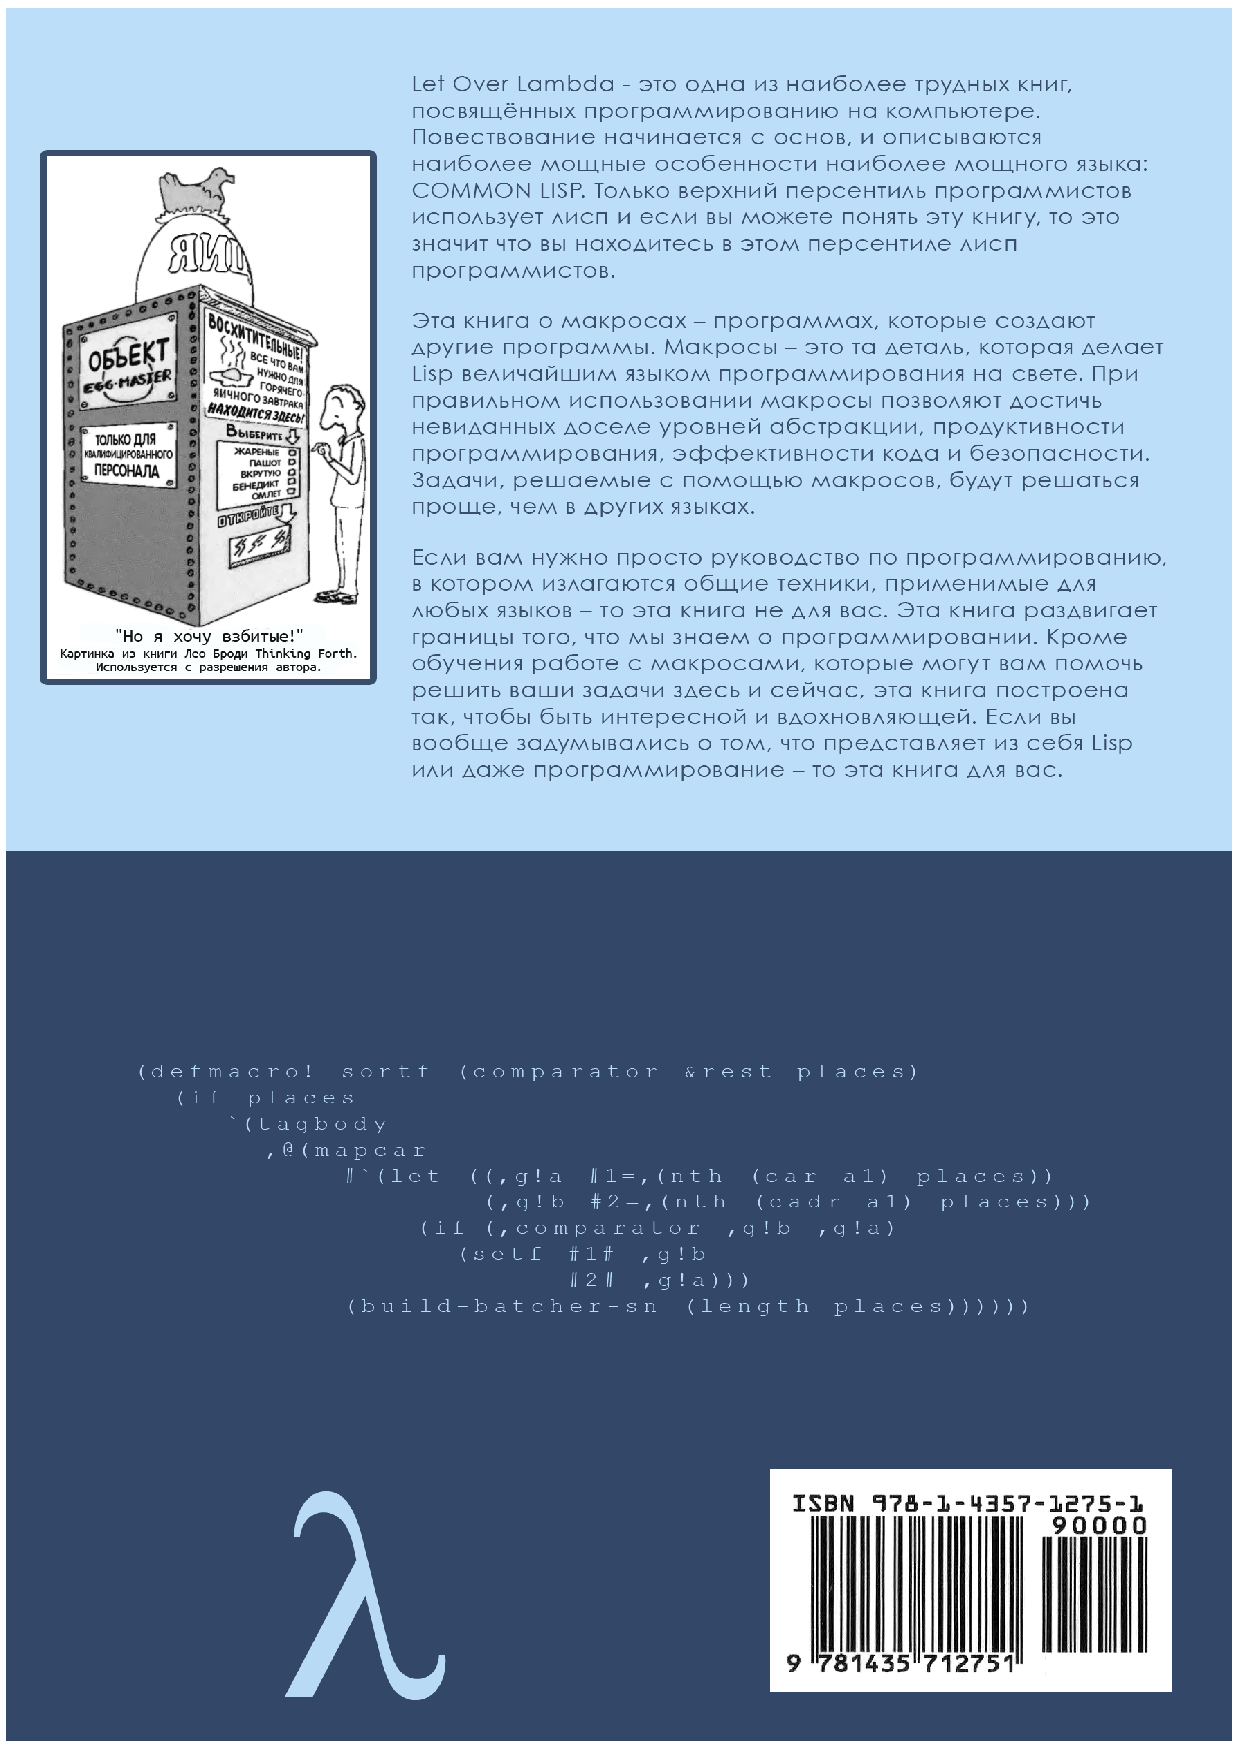
\includepdf[pages={1}]{cover/last_page.pdf}

\end{document}
